%% remember to compile with dvips -t letter for US letter style
\documentclass[acmsmall]{acmart}
%\documentclass[10pt, conference, compsocconf]{IEEEtran}
%\IEEEoverridecommandlockouts

\usepackage{microtype}%if unwanted, comment out or use option "draft"

%\graphicspath{{./graphics/}}%helpful if your graphic files are in another directory

% the recommended bibstyle
\usepackage{amssymb,amsmath,multicol,amsthm}
\usepackage{graphicx,url}
\usepackage{color,setspace,enumitem}
\usepackage{epstopdf}
\usepackage{caption}
%\usepackage{subcaption}
\usepackage{times}
%\usepackage{ulem}
%\usepackage[left=.9in, right=.9in, top=.9in, bottom=.9in]{geometry}
\usepackage{array}
\usepackage{color}

\usepackage[final]{changes}

\usepackage[ruled]{algorithm}
\usepackage{algpseudocode}
\usepackage{ioa_code}
\usepackage{scalerel,stackengine}
\usepackage[symbol]{footmisc}
%Authors' macros
\newtheorem{theorem}{Theorem}
\newtheorem{lemma}[theorem]{Lemma}
\newtheorem{corollary}[theorem]{Corollary}
\newtheorem{remark}[theorem]{Remark}
\newtheorem{definition}[theorem]{Definition}

\newtheorem{claim}[theorem]{Claim}
\newtheorem{proposition}[theorem]{Proposition}
\newtheorem{observation}{Observation}

%\newcommand{\prf}[1]{#1}
\newcommand{\prf}[1]{{}}

%\newtheorem{assert}{Assertion}[section]
%\newenvironment{assertion}{\begin{quote}\begin{assert}}{\end{assert}\end{quote}}

%\newtheorem{invariant}{Invariant}
\newtheorem{property}{Property}

%\newenvironment{proof}{\noindent{\bf Proof.}}{\hfill$\Box$\FF}
\newenvironment{NewProof}{\noindent{\bf Proof.}}{\hfill$\Box$\FF}

%BEGIN DRAWING MACROS
\setlength{\unitlength}{3.4pt}
\newcommand{\drawoval}[5]{
    \put(#1,#2){\oval(#3,#4) \makebox(0,0)[cc]{#5}}}
\newcommand{\drawcenteredtext}[3]{\put(#1,#2){\makebox(0,0){#3}}}
\newcommand{\drawdot}[2]{\put(#1,#2){\circle*{0.5}}}
\newcommand{\drawthickdot}[2]{\put(#1,#2){\circle*{1}}}
\newcommand{\drawvector}[5]{\put(#1,#2){\vector(#4,#5){#3}}}
\newcommand{\drawcircle}[4]{
    \put(#1,#2){\circle{#3}} \put(#1,#2){\makebox(0,0)[cc]{#4}}}
%END DRAWING MACROS

\newcommand{\RTWO}{{\sc Rambo II}}
\newcommand{\RW}[1]{\ms{Reader-Writer}$_{#1}$}
\newcommand{\Recon}[1]{\ms{Recon}$_{#1}$}
\newcommand{\Joiner}[1]{\ms{Joiner}$_{#1}$}
\newcommand{\Elec}[1]{\ms{Elect}$_{#1}$}
\newcommand{\Geo}[1]{\ms{Geo}$_{#1}$}
\newcommand{\Channel}[1]{\ms{Channel}$_{#1}$}
\newcommand{\Cons}{\ms{Cons}}
\newcommand{\HS}[1]{HotSpot$_{#1}$}
\newcommand{\Paxos}{{\sc Paxos}$_{impl}$}
\newcommand{\ltime}[1]{{\ell{\it time}}(#1)}
\renewcommand{\time}[1]{\ms{time}(#1)}
\newcommand{\rr}[1]{$#1$-{\it recon-readiness\/}}
\newcommand{\jc}[1]{$#1$-{\it join-connectivity\/}}
\newcommand{\rs}[1]{$#1$-{\it recon-spacing\/}}
\newcommand{\cv}[1]{$#1$-{\it configuration-viability\/}}

\newtheorem{Def}{Definition}[section]
\newenvironment{Definition}{\begin{Def}\rm}{\hfill$\Box$\end{Def}}

\newcommand{\sacode}[5]
%{ \vspace{.25in} \hrule \vspace{.12in}
{ \vspace{.06in} \hrule \vspace{.06in} %///AS reduce vspace
 \noindent {\bf #1}: \\
 \footnotesize \noindent {\bf Signature:}\B \nobreak
 \normalsize \begin{quote} \nobreak #2 \end{quote}
 \footnotesize \noindent {\bf States:}\B \nobreak
 \begin{quote} \nobreak #3 \end{quote}
 \noindent {\bf Transitions:} \nobreak
 \vspace{-.2in} \nobreak
 \normalsize #4
% \footnotesize \noindent {\bf Tasks:} \nobreak
% \begin{quote} \nobreak #5 \end{quote}
% \normalsize
% \vspace{.12in} \hrule \vspace{.25in}
 \vspace{-.06in} \hrule \vspace{.06in} %///AS reduce vspace
}

\newcommand{\two}[4]{
    \parbox{\columnwidth}{%
    \parbox[t]{#1\columnwidth}{#3}%
    \parbox[t]{#2\columnwidth}{#4}%
}}

\newcommand{\three}[6]{
    \parbox{\columnwidth}{%
    \parbox[t]{#1\columnwidth}{#4}%
    \parbox[t]{#2\columnwidth}{#5}%
    \parbox[t]{#3\columnwidth}{#6}%
}}

\newcommand{\threecolcode}[6]{\BB
 ~\begin{minipage}[t]{#1\textwidth}{\footnotesize ~ #4}\end{minipage}
 \begin{minipage}[t]{#2\textwidth}{\footnotesize ~ #5}\end{minipage}
 \begin{minipage}[t]{#3\textwidth}{\footnotesize ~ #6}\end{minipage}
}

\newcommand{\act}[1]{%
    \relax\ifmmode
        \mathord{\mathcode`\-="702D\sf #1\mathcode`\-="2200}%
    \else
        $\mathord{\mathcode`\-="702D\sf #1\mathcode`\-="2200}$%
%        {\sfshape #1}%
%        {\sf #1}%
    \fi
}

\newcommand{\tup}[1]{%
    \relax\ifmmode
%        \mathord{\mathcode`\-="702D\bf #1\mathcode`\-="2200}%
      \langle #1 \rangle%
    \else
%        $\mathord{\mathcode`\-="702D\bf #1\mathcode`\-="2200}$%
        $\langle$#1$\rangle$%
    \fi
}

\newcommand{\seq}[1]{%
    \relax\ifmmode
%        \mathord{\mathcode`\-="702D\bf #1\mathcode`\-="2200}%
      \langle \! \langle #1 \rangle \! \rangle%
    \else
%        $\mathord{\mathcode`\-="702D\bf #1\mathcode`\-="2200}$%
        $\langle \! \langle$ #1 $\rangle \! \rangle$%
    \fi
}

\newcommand{\twocolcode}[4]{\BB
 ~\begin{minipage}[t]{#1\textwidth}{\footnotesize ~ #3}\end{minipage}
 \begin{minipage}[t]{#2\textwidth}{\footnotesize ~ #4}\end{minipage}
}

\newcommand{\B}{\vspace*{-\smallskipamount}}
\newcommand{\BB}{\vspace*{-\medskipamount}}
\newcommand{\BBB}{\vspace*{-\bigskipamount}}
\newcommand{\F}{\vspace*{\smallskipamount}}
\newcommand{\FF}{\vspace*{\medskipamount}}
\newcommand{\FFF}{\vspace*{\bigskipamount}}
\newcommand{\T}{\hspace*{1em}}
\newcommand{\TT}{\hspace*{2em}}
\newcommand{\TTT}{\hspace*{3em}}
\newcommand{\NT}{\hspace*{-1em}}
%\newcommand{\Item}{\vspace*{-1.5\smallskipamount}\item}
%\newcommand{\Item}{\vspace*{-2.5\smallskipamount}\item}
\newcommand{\Item}{\item}
%\setlength{\leftmargini}{1.5em}
%\setlength{\leftmarginii}{1.6em}

\newcommand{\Section}[1]{\section{#1}}%{\BB\section{#1}\BB} %{\B\section{#1}\B}
\newcommand{\Subsection}[1]{\subsection{#1}}%{\BB\subsection{#1}\BB} %{\B\subsection{#1}\B}
\newcommand{\Subsubsection}[1]{\subsubsection{#1}}%{\BB\subsubsection{#1}}
\newcommand{\Paragraph}[1]{\paragraph{#1}}%{\BB\BB\paragraph{#1}}

\newcommand{\Nat}{{\N}}
\newcommand{\N}{\mathbb N}
\newcommand{\R}{\mathbb R}
\newcommand{\nnr}{{\mathbb R}^+}
\newcommand{\rip}{\pm}
\newcommand{\Cbot}{C_{\bot}}
\newcommand{\EXP}[1]{{\mathbb E}\left(#1\right)}
\newcommand{\Prob}[1]{{\mathbf P}{\mathbf r}\left(#1\right)}
\newcommand{\Var}[1]{Var\left(#1\right)}

\newcommand{\RAMBO}[1]{{\sc Rambo}$_{#1}$}
\newcommand{\ACK}{ack}
\newcommand{\ms}[1]{%
    \relax\ifmmode
        \mathord{\mathcode`\-="702D\it #1\mathcode`\-="2200}%
    \else
%        $\mathord{\mathcode`\-="702D\it #1\mathcode`\-="2200}$%
%        {\itshape #1}%
        {\it #1}%
    \fi
}

%NEW MACRO USED FOR MESSAGE HEADERS
\newcommand{\lit}[1]{%
    \relax\ifmmode
        \mathord{\mathcode`\-="702D\sf #1\mathcode`\-="2200}%
    \else
%        $\mathord{\mathcode`\-="702D\sf #1\mathcode`\-="2200}$%
%        {\itshape #1}%
        {\it #1}%
    \fi
}

\newcommand{\XA}[1]{#1} % To remove stuff from extended Abstract
\newcommand{\XD}[1]{#1} % To remove stuff for DISC submission
\newcommand{\XDK}[1]{}% To keep stuff for DISC final
\newcommand{\remove}[1]{} % To remove stuff
\newcommand{\proofremove}[1]{} % To remove stuff
\newcommand{\uselater}[1]{} % To remove stuff
\newcommand{\viable}[1]{$#1${\it -viable\/}}

% overladed latex command
\renewcommand{\setminus}{-}

% shorthand mnemonics
% ig with phase number
\newcommand{\igwsntp}[3]{\ms{ig({#1})_{#2}.w-sent({#3})}}
\newcommand{\igdsntp}[3]{\ms{ig(#1)_{#2}.d-sent(#3)}}

% ig without phase number
\newcommand{\wknow}{\ms{w-known}}
\newcommand{\igwknow}[2]{\ms{ig(#1)_{#2}.\wknow}}
\newcommand{\dknow}{\ms{d-known}}
\newcommand{\igdknow}[2]{\ms{ig(#1)_{#2}.\dknow}}

\newcommand{\wunack}{\ms{w-unack}}
\newcommand{\igwunack}[2]{\ms{ig(#1)_{#2}.\wunack}}
\newcommand{\dunack}{\ms{d-unack}}
\newcommand{\igdunack}[2]{\ms{ig(#1)_{#2}.\dunack}}
\newcommand{\igpack}[2]{\ms{ig(#1)_{#2}.\ms{p-ack}}}

\newcommand{\hmsg}[1]{\ms{h-msg}_{#1}}
\newcommand{\hMSG}{\ms{h-MSG}}
\newcommand{\oMSG}{\tup{W,v,t,cm,pns,pnr}}
\newcommand{\MSG}{\tup{W,v,t,cm,\ms{pm}}}
\newcommand{\HV}{{[h]}}

%old notation
\newcommand{\wdtp}[1]{\ms{w-sent(#1)}}
\newcommand{\ddtp}[1]{\ms{d-sent(#1)}}

%history variables
\newcommand{\hrW}[1]{\ms{hrecv-W(#1)}}
\newcommand{\hsW}[1]{\ms{hsent-W(#1)}}
\newcommand{\hrD}[1]{\ms{hrecv-D(#1)}}
\newcommand{\hsD}[1]{\ms{hsent-D(#1)}}
\newcommand{\hsunack}[1]{\ms{hs-wunack(#1)}}
\newcommand{\hsdunack}[1]{\ms{hs-dunack(#1)}}
\newcommand{\hsknow}[1]{\ms{hs-wknow(#1)}}
\newcommand{\hsdknow}[1]{\ms{hs-dknow(#1)}}
\newcommand{\hsp}[1]{\ms{hs-pack(#1)}}
\newcommand{\hsworld}[1]{\ms{hs-world(#1)}}
\newcommand{\hsdep}[1]{\ms{hs-departed(#1)}}
%\newcommand{\hknw}[2]{\ms{h-know(#1,#2)}}

\newcommand{\MSGr}{$MSG_{{\scriptscriptstyle \mathrm{RA}}}$}
\newcommand{\MSGl}{$MSG_{{\scriptscriptstyle \mathrm{LR}}}$}
\newcommand{\MSGi}{$MSG_{{\scriptscriptstyle \mathrm{IG}}}$}

\newcommand{\n}{\hat{n}}
%\newcommand{\IGR}[1]{{\sc IG}-\RAMBO{{#1}}}
%\newcommand{\IGR}[1]{{\rm IG-}\RAMBO{{#1}}}
\newcommand{\IGR}[1]{{\sc Atila{#1}}}
\newcommand{\HR}[1]{{\sc H}-\RAMBO{{#1}}}

\newcommand{\world}{\ms{world}}

\newcommand{\peter}[1]{\textcolor{red}{{\bf (Peter:)} #1}}
\newcommand{\cgc}[1]{#1}%{\textcolor{blue}{{\bf (CG:)} #1}}
%\newcommand{\elaine}[1]{\textcolor{magenta}{{\bf (Elaine:)} #1}}
\newcommand{\cg}[1]{#1}%{\textcolor{blue}{{#1}}}
\newcommand{\red}[1]{\textcolor{red}{{#1}}}
\newcommand{\blue}[1]{\textcolor{blue}{{#1}}}

%\renewcommand{\baselinestretch}{0.94}
%\renewcommand{\baselinestretch}{1.10}


\newcommand{\point}[1]{~\\\smallskip\noindent {\tt (*)} #1} %\item #1}

\newcommand{\ef}[2]{
    \begin{tabbing}
    XX\= XX\=XX\=XX\=XX\=XX\=  \kill
    \protect #1\\
    ~ Effect: \+ \\
      #2 \- 
\end{tabbing}}

\newcommand{\prcef}[3]{
    \begin{tabbing}
    XX\= XX\=XX\=XX\=XX\= \kill
    \protect #1\\
    ~ Precondition: \+ \\
     #2 \- \\
    ~ Effect: \+ \\
     #3 \- 
\end{tabbing}}

\newenvironment{mylisting}
{\begin{list}{}{\setlength{\leftmargin}{1em}}\item\scriptsize\bfseries}
{\end{list}}

\newenvironment{mytinylisting}
{\begin{list}{}{\setlength{\leftmargin}{1em}}\item\tiny\bfseries}
{\end{list}}

  

%%%%%%%%%%%%%%%%%%%%%%%%%%%%%%%%%%%%%%%%%%%%%%
%%%%%% FORMATTING 
%%%%%%%%%%%%%%%%%%%%%%%%%%%%%%%%%%%%%%%%%%%%%%
\newcommand{\case}[1]{
        {\vspace{1em}\noindent{\bf Case #1:}}}
\newcommand{\subcase}[1]
	{{\emph{Case #1:}}}

%Efficiency Metric
\newcommand{\efficiency}{operation latency}

%floor
\newcommand{\floor}[1]{\left\lfloor #1 \right\rfloor}
%ceiling
\newcommand{\ceil}[1]{\lceil #1 \rceil}


%%%%%%%%%%%%%%%%%%%%%%%%%%%%%%%%%%%%%%%%%%%%%%
%%%%%% LIST OF SYMBOLS
%%%%%%%%%%%%%%%%%%%%%%%%%%%%%%%%%%%%%%%%%%%%%%

% Define List of Symbols
% Added by Nicolas Nicolaou
\makeatletter
\def\mainlistofsymbols{
  %\newpage
  %\vspace{.25in}
  %\begin{center}
  %  {\Large\bf LIST OF SYMBOLS}
  %\end{center}
  \normalsize
  \vspace*{1.5 em}
  \@starttoc{los}
}

\def\partonelistofsymbols{
  \normalsize
  \vspace*{1.5 em}
  \@starttoc{p1los}
}

\def\parttwolistofsymbols{
  \normalsize
  \vspace*{1.5 em}
  \@starttoc{p2los}
}

%% Define the formatting of the symbol entry in the addcontentsline command : NN
\def\l@symbol#1#2{\addpenalty{-\@highpenalty} \vskip 4pt plus 2pt
{\@dottedtocline{0}{0em}{8em}{#1}{#2}}}
\makeatother

% Command for list of symbols
%% The symbol appears in both the los and in place in the text : NN
\newcommand{\mainsym}[2]{%
#1%
\addcontentsline{los}{symbol}{\protect\numberline{#1}{#2}}
%\addtocontents{los}{\contentsline{symbol}{\protect\numberline{#1}{#2}}{}}
}

%% The symbol appears in both the los and in place in the text : NN
\newcommand{\partonesym}[2]{%
#1%
\addcontentsline{p1los}{symbol}{\protect\numberline{#1}{#2}}
}

%% The symbol appears in both the los and in place in the text : NN
\newcommand{\parttwosym}[2]{%
#1%
\addcontentsline{p2los}{symbol}{\protect\numberline{#1}{#2}}
}

%% The symbol does not appear in the text but only in the los : NN
\newcommand{\newhiddensym}[2]{%
%% NN uncomment next line to work
%\addcontentsline{los}{symbol}{\protect\numberline{#1}{#2}}
}




%%%%%%%%%%%%%%%%%%%%%%%%%%%%%%%%%%%%%%%%%%%%%%
%IOA
%%%%%%%%%%%%%%%%%%%%%%%%%%%%%%%%%%%%%%%%%%%%%%
\newcommand{\stateSet}[1]{states(#1)}
\newcommand{\startSet}[1]{start(#1)}
\newcommand{\actionSet}[1]{actions(#1)}
\newcommand{\inputSet}[1]{in(#1)}
\newcommand{\outputSet}[1]{out(#1)}
\newcommand{\internalSet}[1]{int(#1)}
\newcommand{\sigSet}[1]{sig(#1)}
\newcommand{\extsigSet}[1]{extsig(#1)}
\newcommand{\transSet}[1]{trans(#1)}
% Automata
\newcommand{\IOA}{A}
\newcommand{\algIOA}[2]{\ifmmode{\text{#1}_{#2}}\else{$\text{#1}_{#2}$}\fi}
% IOA assigned to process #1
\newcommand{\prIOA}[1]{A_{#1}}
\newcommand{\chIOA}[1]{\text{\sc Channel}_{#1}}
\newcommand{\rdIOA}[2]{\algIOA{#1}{#2}}
\newcommand{\wrtIOA}[2]{\algIOA{#1}{#2}}
\newcommand{\srvIOA}[2]{\algIOA{#1}{#2}}
% Memory Automaton
\newcommand{\memIOA}{\mathcal{M}}
% Algorithm Automata
\newcommand{\abdIOA}[1]{\algIOA{\ABD}{#1}}
\newcommand{\fastIOA}[1]{\algIOA{\fast}{#1}}
\newcommand{\sliqIOA}[1]{\algIOA{\SLIQ}{#1}}
\newcommand{\cwfrIOA}[1]{\algIOA{\cwfr}{#1}}
\newcommand{\sfwIOA}[1]{\algIOA{\sfw}{#1}}

%%%%%%%%%%%%%%%%%%%%%%%%%%%%%%%%%%%%%%%%%%%%%%
% Executions and execution fragments
%%%%%%%%%%%%%%%%%%%%%%%%%%%%%%%%%%%%%%%%%%%%%%
\newcommand{\EX}{\ifmmode{\xi}\else{$\xi$}\fi}
\newcommand{\EXF}{\ifmmode{\phi}\else{$\phi$}\fi}
%Extend
\newcommand{\extend}[2]{#1\circ#2}
%Extracted execution
\newcommand{\extract}[2]{#1|#2}
%Actions
\newcommand{\acts}{\alpha}
%Execution Set
\newcommand{\execSet}[1]{execs(#1)}
%Good Executions Set for a particular failure pattern
\newcommand{\gexecSet}[2]{goodexecs(#1,#2)}
%General Good Executions Set
\newcommand{\ggexecSet}[1]{goodexecs(#1)}
%Event History
\newcommand{\hist}[1]{H_{#1}}
%Event History Fragment
\newcommand{\histf}[1]{H_{#1}}

%%%%%%%%%%%%%%%%%%%%%%%%%%%%%%%%%%%%%%%%%%%%%%
% States and State Variables
%%%%%%%%%%%%%%%%%%%%%%%%%%%%%%%%%%%%%%%%%%%%%%
%State of an automaton
%\newcommand{\st}{\sigma}
\newcommand{\state}{\sigma}
% Invocation Step
\newcommand{\invStep}[1]{inv(#1)}
\newcommand{\stInv}[1]{\st_{\invStep{#1}}}
% Response Step
\newcommand{\resStep}[1]{res(#1)}
\newcommand{\stRes}[1]{\st_{\resStep{#1}}}
%The value of variable #2 in state #1 of process #2 
\newcommand{\stVar}[3]{#1[#2].#3}
%Fix events (read, write, inform)
\newcommand{\stfix}[1]{\st_{fix(#1)}}

%%%%%%%%%%%%%%%%%%%%%%%%%%%%%%%%%%%%%%%%%%%%%%
% Object Type Notation
%%%%%%%%%%%%%%%%%%%%%%%%%%%%%%%%%%%%%%%%%%%%%%
%Object Response Set
\newcommand{\objResSet}[1]{\Gamma_{#1}}
%Object Operation Set
\newcommand{\objOpSet}[1]{\opSet_{#1}}
%Object State Set
\newcommand{\objStSet}[1]{\Sigma_{#1}}
%Object Transition Set
\newcommand{\objTSet}[1]{\Delta_{#1}}
%Object
\newcommand{\obj}[1]{O_{#1}}

%%%%%%%%%%%%%%%%%%%%%%%%%%%%%%%%%%%%%%%%%%%%%%
% Quorum systems
%%%%%%%%%%%%%%%%%%%%%%%%%%%%%%%%%%%%%%%%%%%%%%
\newcommand{\qs}{\mathbb{Q}}
% Biquorum System
\newcommand{\bs}{\mathbb{B}}
% Sub-Quorum system 
\newcommand{\subqs}[1]{\qs^{#1}}
% Quorum
\newcommand{\quo}[1]{Q_{#1}}
% Intersection
\newcommand{\inter}[1]{
	\ifmmode{\left(\bigcap_{\mathcal{Q}\in#1}\mathcal{Q}\right)}
	\else{$\left(\bigcap_{\mathcal{Q}\in#1}\mathcal{Q}\right)$}
	\fi
}
%Intersection Degree
\newcommand{\qsdeg}{\delta}

%%%%%%%%%%%%%%%%%%%%%%%%%%%%%%%%%%%%%%%%%%%%%%
%Identifier sets
%%%%%%%%%%%%%%%%%%%%%%%%%%%%%%%%%%%%%%%%%%%%%%
\newcommand{\idSet}{\mathcal{I}}
%Writer set
\newcommand{\wSet}{\mathcal{W}}
%Readers set
\newcommand{\rdSet}{\mathcal{R}}
% Reconfigurators Set
\newcommand{\recSet}{\mathcal{G}}
%Servers Set
\newcommand{\srvSet}{\mathcal{S}}
%Directory Servers Set
\newcommand{\dirSet}{\mathcal{D}}
%Replica Servers Set
\newcommand{\repSet}{\mathcal{R}}
%File Managers Servers Set
\newcommand{\manSet}{\mathcal{M}}
%Failure Set
\newcommand{\failSet}[1]{\mathcal{F}_{#1}(A)}
%Failure Model
\newcommand{\failModel}[1]{fail(#1)}
%Virtual Node Set
\newcommand{\vSet}{\mathcal{V}}
%Objects set
\newcommand{\objSet}{\mathcal{O}}
% Version Set
\newcommand{\verSet}{\mathit{Versions}}
% Operation Set
\newcommand{\opSet}{\Pi}
%  Client Set
\newcommand{\cSet}{\mathcal{I}}

%%%%%%%%%%%%%%%%%%%%%%%%%%%%%%%%%%%%%%%%%%%%%%
% Configuration Notation
%%%%%%%%%%%%%%%%%%%%%%%%%%%%%%%%%%%%%%%%%%%%%%
% Configuration Set
\newcommand{\confSet}{\mathcal{C}}
% Servers in a configuration
\newcommand{\servers}[1]{ #1.Servers}
%Configuration quorums
\newcommand{\quorums}[1]{ #1.Quorums}
% Configuration consensus object
\newcommand{\consensus}[1]{ #1.Con}


%%%%%%%%%%%%%%%%%%%%%%%%%%%%%%%%%%%%%%%%%%%%%%
% Operation Notation
%%%%%%%%%%%%%%%%%%%%%%%%%%%%%%%%%%%%%%%%%%%%%%
\newcommand{\op}{\pi}
% Traceable Operation
\newcommand{\trop}[2]{\op(#1)[#2]}

%Read operation
\newcommand{\rd}{\rho}
%Write operation
\newcommand{\wrt}{\omega}

%Unique write operation
\newcommand{\rf}{\mathfrak{R}}
%Update operation
\newcommand{\upd}{\mathfrak{u}}

\mathchardef\mhyphen="2D
% Write on Traceable Register
\newcommand{\trw}[2]{\act{tr-write}(#1)[#2]}
% Read on Traceable Register
\newcommand{\trrd}[2]{\act{tr-read}(#1)[#2]}
% Write on Ranked Register
\newcommand{\rrw}[2]{rr\mhyphen\wrt(#1)[#2]}
% Read on Ranked Register
\newcommand{\rrrd}[2]{rr\mhyphen\rd(#1)[#2]}


%%%%%%%%%%%%%%%%%%%%%%%%%%%%%%%%%%%%%%%%%%%%%%
% Processes
%%%%%%%%%%%%%%%%%%%%%%%%%%%%%%%%%%%%%%%%%%%%%%
\newcommand{\pr}{p}
%Reader
\newcommand{\rdr}{r}
%Writer
\newcommand{\wrtr}{w}
%Server
\newcommand{\srvr}{s}
% Reconfigurer
\newcommand{\rec}{rc}

%Operation Precedence
\newcommand{\bef}{\rightarrow}
\newcommand{\conc}{\leftrightarrow}

%Techniques Notation
%Virtual Node ID for a reader
\newcommand{\vid}[1]{\ifmmode{\nu_{#1}}\else{$\nu_{#1}$}\fi}
%\newcommand{\vid}[1]{\nu(#1)}
\newcommand{\id}[2]{\tup{#1,#2}}
%Quorum Views
\newcommand{\qv}[1]{{\bf QV#1}}
%Server Side Ordering
\newcommand{\SSO}{{\sc SSO}}
%In progress set
\newcommand{\inps}[1]{\ms{inprogress}_{#1}}
%Seen Set
\newcommand{\seen}{\ifmmode{seen}\else{$seen$}\fi}
%Number of failures
\newcommand{\fnum}{f}

%%%%%%%%%%%%%%%%%%%%%%%%%%%%%%%%%%%%%%%%%%%%%%
% Algorithm Names
%%%%%%%%%%%%%%%%%%%%%%%%%%%%%%%%%%%%%%%%%%%%%%

%Semifast
\newcommand{\SF}{{\sc Sf}}
%Quorum Views (Sliq)
\newcommand{\SLIQ}{{\sc Sliq}}
%Classic writes Fast reads
\newcommand{\cwfr}{{\sc CwFr}}
%Server Side Ordering
\newcommand{\sfw}{{\sc SfW}}
%Approximate Server Side Ordering
\newcommand{\aprxsfw}{{\sc aprx-SfW}}
%ABD
\newcommand{\ABD}{{\sc ABD}}
%MW-ABD
\newcommand{\mwABD}{{\sc mw}\ABD{}}
%Fast
\newcommand{\fast}{{\sc Fast}}
%Erasure COded ABD
\newcommand{\ecoABD}{{\sc eco}-\ABD{}}
%Erasure COded Fast
\newcommand{\ecofast}{{\sc eco}-\fast{}}
%Erasure COded Quorum Views
\newcommand{\ecocwfr}{{\sc eco}-\cwfr{}}
%Atomic Reconfigurable Erasure coded Storage
\newcommand{\ares}{{\sc Ares}}
%Flexible Erasure Coded Algorithm
\newcommand{\flexCAS}{{\sc TREAS}}

%%%%%%%%%%%%%%%%%%%%%%%%%%%%%%%%%%%%%%%%%%%%%%
% Register Characteristics
%%%%%%%%%%%%%%%%%%%%%%%%%%%%%%%%%%%%%%%%%%%%%%

%Object/File set
\newcommand{\fileSet}{F}
%Value Set
\newcommand{\valSet}{{\mathcal V}}
%Register Set
\newcommand{\regSet}{X}
%Timestamp Set
\newcommand{\tsSet}{{\mathcal T}}
%Message Set
\newcommand{\msgSet}{M}
%Message
\newcommand{\msg}[1]{m_{#1}}
%Value
\newcommand{\val}[1]{val_{#1}}
%New Value
\newcommand{\newv}{v}
%Previous Value (SF, SLIQ)
\newcommand{\prev}{vp}

%%%%%%%%%%%%%%%%%%%%%%%%%%%%%%%%%%%%%%%%%%%%%%
% Timestamp & Tags
%%%%%%%%%%%%%%%%%%%%%%%%%%%%%%%%%%%%%%%%%%%%%%
%Timestamp of process #1
\newcommand{\ts}[1]{ts_{#1}}
%Timestamp sent by a process #1 for an operation #2
\newcommand{\msgts}[2]{\msgop{#1}{#2}.\ts{}}
\newcommand{\tsop}[2]{\stVar{\stRes{#2}}{#1}{\ts{}}}
%Postit of process #1
\newcommand{\ps}[1]{postit_{#1}}
%Postit sent by a process #1 for an operation #2
\newcommand{\psop}[2]{postit_{#1}(#2)}
%Tag of process #1
\newcommand{\tg}[1]{\tau_{#1}}
\newcommand{\msgtg}[2]{\msgop{#1}{#2}.\tg{}}
%Tag returned by a process to an operation
\newcommand{\tgop}[2]{\stVar{\stRes{#2}}{#1}{\tg{}}}
%max timestamp, tag and postit
\newcommand{\maxts}[1]{\ifmmode{maxTS_{#1}}\else{$maxTS_{#1}$}\fi}
\newcommand{\maxtag}[1]{\ifmmode{maxTag_{#1}}\else{$maxTag_{#1}$}\fi}
\newcommand{\maxpair}[1]{\ifmmode{maxMPair_{#1}}\else{$maxMPair_{#1}$}\fi}
\newcommand{\mintag}[1]{\ifmmode{minTag_{#1}}\else{$minTag_{#1}$}\fi}
\newcommand{\maxps}{\ifmmode{maxPS}\else{$maxPS$}\fi}
\newcommand{\conftg}[1]{\ifmmode{confirmed_{#1}}\else{$confirmed_{#1}$}\fi}
\newcommand{\maxconftag}{\ifmmode{\ms{maxCT}}\else{$maxCT$}\fi}
%Max timestamp at read event of read operation
\newcommand{\startmax}[2]{\stVar{\stInv{#2}}{#1}{\maxts{}}}
%Max timestamp at read-fix evernt of read operation 
%\newcommand{\witmax}[1]{\act{witnessed-maxTs}(#1)}
%Max tag at read event of read operation
%\newcommand{\startmaxtg}[1]{\act{start-maxTag}(#1)}
%Max tag at read-fix evernt of read operation 
%\newcommand{\witmaxtg}[1]{\act{witnessed-maxTag}(#1)}
%Min tag at read-fix evernt of read operation 
%\newcommand{\witmintg}[1]{\act{witnessed-maxTag}(#1)}
%Starting timestamp at read event of read operation 
%\newcommand{\startts}[2]{start(\ts{#1}(#2))}
%Starting tag at read event of read operation 
\newcommand{\starttag}[2]{\stVar{\stInv{#2}}{#1}{\tg{}}}

%%%%%%%%%%%%%%%%%%%%%%%%%%%%%%%%%%%%%%%%%%%%%%
% Semifast Variables
%%%%%%%%%%%%%%%%%%%%%%%%%%%%%%%%%%%%%%%%%%%%%%
%seen set of server #2 in state #1
\newcommand{\stateseen}[2]{#1[#2].\seen}
%Set of servers that reply with maxPS to operation #1
\newcommand{\maxpsSet}[1]{PS_{#1}}
%Set of server replies
\newcommand{\ackSet}[1]{srvAck(#1)}
%Set of server replies to operation #1
\newcommand{\psSet}[1]{srvInf(#1)}
%Set of servers that replied with maxTs to operation #1
\newcommand{\maxsrvSet}[1]{maxTsSrv(#1)}
%Set of messages that contained maxTs
\newcommand{\maxmsgSet}[1]{maxTsMsg(#1)}
% read predicate
\newcommand{\semirp}{{\bf SF-RP}}
% Predicate factor
\newcommand{\sffactor}{\beta}

%%%%%%%%%%%%%%%%%%%%%%%%%%%%%%%%%%%%%%%%%%%%%%
% SLIQ notation
%%%%%%%%%%%%%%%%%%%%%%%%%%%%%%%%%%%%%%%%%%%%%%
%Extention of execution #1
\newcommand{\extex}[1]{\Delta(#1)}

%%%%%%%%%%%%%%%%%%%%%%%%%%%%%%%%%%%%%%%%%%%%%%
% CWFR variables
%%%%%%%%%%%%%%%%%%%%%%%%%%%%%%%%%%%%%%%%%%%%%%
\newcommand{\rquo}{replyQ}
\newcommand{\quotg}[2]{(#1)^{>#2}}

%%%%%%%%%%%%%%%%%%%%%%%%%%%%%%%%%%%%%%%%%%%%%%
% ARES variables
%%%%%%%%%%%%%%%%%%%%%%%%%%%%%%%%%%%%%%%%%%%%%%
% Reconfiguration Box
\newcommand{\recBox}{{\it\bf RecBox}}

%%%%%%%%%%%%%%%%%%%%%%%%%%%%%%%%%%%%%%%%%%%%%%
% Server Side Ordering
%%%%%%%%%%%%%%%%%%%%%%%%%%%%%%%%%%%%%%%%%%%%%%
%write Counter
\newcommand{\wc}{wc}
% Confirmed variable of server #1 for operation #2
\newcommand{\conf}[2]{\msgop{#1}{#2}.\conftg{}}
% Inprogress set of process #1 for operation #2
\newcommand{\inp}[2]{\msgop{#1}{#2}.\inps{}}
% Tag found in the in-progress set of a message
\newcommand{\minptg}[3]{\msgop{#1}{#2}.\inps{}[#3].\tg{}}
% Tag found in the in-progress set
\newcommand{\tginp}[3]{\stVar{{#1}}{#2}{\inps{}[#3].\tg{}}}

%%%%%%%%%%%%%%%%%%%%%%%%%%%%%%%%%%%%%%%%%%%%%%
% Communication
%%%%%%%%%%%%%%%%%%%%%%%%%%%%%%%%%%%%%%%%%%%%%%
%%% Messages
%message sent from a process #1 for operation #2
\newcommand{\msgop}[2]{m(#2)_{#1}}
%Read \rd_{#1} perform its #2 communication round
\newcommand{\rdf}[2]{\rd_{#1}^{#2}}
%Write \wrt_{#1} perform its #2 communication round
\newcommand{\wrtf}[2]{\wrt_{#1}^{#2}}
%Set of servers that reply to operation #1
\newcommand{\replySet}[1]{\srvSet_{#1}}

%%% Quorum Communication
%Contact definition
\newcommand{\contact}[3]{cnt(#3,#2)_{#1}}
%Strictly Contacts
\newcommand{\scontact}[3]{scnt(#3,#2)_{#1}}


%%%%%%%%%%%%%%%%%%%%%%%%%%%%%%%%%%%%%%%%%%%%%%
%% ABBREVIATIONS
%%%%%%%%%%%%%%%%%%%%%%%%%%%%%%%%%%%%%%%%%%%%%%
%Communication round
\newcommand{\comr}{round}%{\sc CR}}

% Read/Write
\newcommand{\rw}{{\sc read/write}}

%single writer single reader 
\newcommand{\swsr}{{\sc swsr}}
%single writer multiple reader 
\newcommand{\swmr}{{\sc swmr}}
%multiple writer single reader 
\newcommand{\mwsr}{{\sc mwsr}}
%multiple writer multiple reader 
\newcommand{\mwmr}{{\sc mwmr}}

%%%%%%%%%%%%%%%%%%%%%%%%%%%%%%%%%%%%%%%%%%%%%%
%% Helper Commands (comments, removals etc.)
%%%%%%%%%%%%%%%%%%%%%%%%%%%%%%%%%%%%%%%%%%%%%%
%\newcommand{\remove}[1]{}




\definechangesauthor[name=Nicolas, color=red]{NN}
\definechangesauthor[name=Viveck, color=green]{VC}
\definechangesauthor[name=Kishori, color=blue]{KK}

\newcommand{\nnfix}[1]{{\color{black} #1}}
\newcommand{\myemph}[1]{{\it #1}}
%\newcommand{\nn}[1]{{\red{#1}}}
\newcommand{\nn}[1]{\added[id=NN]{#1}}
%\newcommand{\nnrev}[2]{\sout{}{\blue{#2}}}
\newcommand{\nnrev}[2]{\replaced[id=NN]{#2}{#1}}
%\newcommand{\kmk}[1]{{\red{#1}}}
\newcommand{\kmkrev}[2]{\replaced[id=KK]{#1}{#2}}
\newcommand{\kmk}[1]{\added[id=KK]{#1}}
\newcommand{\kmkremove}[1]{{\color{red}[\sout{#1}]}}
%\renewcommand{\cg}[1]{{\textcolor{blue}{#1}}}
\newcommand{\vc}[1]{\added[id=VC]{#1}}
\newtheorem*{theorem*}{{\bf Theorem}}
\newtheorem*{lemma*}{{\bf Lemma}}


  %\newcommand{\myparagraph}[1]{\paragraph*{#1}}
\newcommand{\myparagraph}[1]{\smallskip\noindent{\textbf{#1}}}
%Coding Stuff
\newcommand{\states}[1]{{ {states}(#1)}}
\newcommand{\startstates}[1]{{ {start}(#1)}}
\newcommand{\sig}[1]{{ {sig}(#1)}}
\newcommand{\inactions}[1]{{ {in}(#1)}}
\newcommand{\outactions}[1]{{ {out}(#1)}}
\newcommand{\intactions}[1]{{ {int}(#1)}}
\newcommand{\extactions}[1]{{ {ext}(#1)}}
\newcommand{\trans}[1]{{ {trans}(#1)}}
\newcommand{\encode}[3]{{ {encode}_{#1, #2}(#3)}}
\newcommand{\decode}[3]{{ {decode}_{#1, #2}(#3)}}
\newcommand{\cvec}[2]{\mathbf{c}^{#1}_{#2}}
\newcommand{\atT}[2]{#1|_{#2}}
\newcommand{\status}[1]{#1.status}
\newcommand{\config}[1]{#1.cfg}
%\newcommand{\CASOPT}{{\sc TREAS}} 
%\renewcommand{\baselinestretch}{.95} 
\newcommand{\GetTag}{{ \it{get-tag}}}
\newcommand{\QueryTag}{\text{\sc{query-tag}}}
\newcommand{\PutData}{{ \it{put-data}}}
\newcommand{\PutDataTag}{\text{\sc{put-data}}}
\newcommand{\GetData}{{ \it{get-data}}}
\newcommand{\QueryTagData}{\text{\sc{query-tag-data}}}
\newcommand{\GetTagResp}{{ \it{get-tag-resp}}}
\newcommand{\GetDataResp}{{ \it{get-data-resp}}}
\newcommand{\PutDataResp}{{ \it{put-data-resp}}}
\newcommand{\InitRep}{{ \it{init-repair}}}
 \newcommand{\RepairTagData}{\text{\sc{repair-tag-data}}}
\newcommand{\InitRepResp}{{ \it{init-repair-resp}}}
\newcommand{\CodedElementTag}{\text{\sc{code-elements}}}
\newcommand{\Coded}{code\act{-}elems}
\newcommand{\ConfirmDataTag}{\text{\sc{confirm-data}}}
\newcommand{\QueryList}{\text{\sc{query-list}}}
\newcommand{\RepairList}{\text{\sc{repair-list}}}
\newcommand{\optag}[1]{{tag(#1)}}
\newcommand{\gseq}{{\mathcal{G}_L}}

\newcommand{\smdelay}{d}
\newcommand{\lgdelay}{D}
\newcommand{\opdelay}[1]{T(#1)}
\newcommand{\opdelaymin}[1]{T_{min}(#1)}
\newcommand{\opdelaymax}[1]{T_{max}(#1)}
\newcommand{\seqlen}{\lambda}
\newcommand{\dap}[1]{{DAP(#1)}}

\algblockdefx[Operation]{Operation}{EndOperation}%
[2]{{\bf operation} $\act{#1}$(#2)}%
{{\bf end operation}}
\algblockdefx[Procedure]{Procedure}{EndProcedure}%
[2]{{\bf procedure} $\act{#1}$(#2)}%
{{\bf end procedure}}
\algblockdefx[Receive]{Receive}{EndReceive}%
[2]{{\bf Upon receive} (#1)$_{\text{ #2 }}${\bf from} $q$}%
{{\bf end receive}}


\newcommand\wwidehat[1]{%
\savestack{\tmpbox}{\stretchto{%
  \scaleto{%
    \scalerel*[\widthof{\ensuremath{#1}}]{\kern-.6pt\bigwedge\kern-.6pt}%
    {\rule[-\textheight/2]{1ex}{\textheight}}%WIDTH-LIMITED BIG WEDGE
  }{\textheight}% 
}{0.5ex}}%
\stackon[1pt]{#1}{\tmpbox}%
}

\newcommand{\daputdata}[2]{ {#1}.{\act{put-data}(#2)}}
\newcommand{\dagetdata}[1]{ {#1}.{\act{get-data}()}}
\newcommand{\dagettag}[1]{ {#1}.{\act{get-tag}()}}
\newcommand{\treas}{{\sc Treas}}
\newcommand{\aresopt}{{\sc ares-opt}}
\newcommand{\algo}[1]{{#1}.A}


\renewcommand{\thefootnote}{\fnsymbol{footnote}}
\newcommand{\cseq}[1]{\widehat{#1}}
\newcolumntype{P}[1]{>{\centering\arraybackslash}p{#1}}

%\begin{titlepage}

\title{
	\ares{}:  Adaptive,  Reconfigurable,  Erasure coded, atomic  Storage 	
}


\author{Nicolas Nicolaou}
\email{nicolas@algolysis.com}
\affiliation{Algolysis Ltd, Limassol, Cyprus}
\author{Viveck Cadambe}
\email{vxc12@engr.psu.edu}
\affiliation{EE Department, Penn.  State University, University Park, PA, US}
\author{N. Prakash} 
\email{prakashn@mit.edu}
\author{Kishori M. Konwar}
\email{kishori@csail.mit.edu}
\author{Muriel Medard}
\email{medard@mit.edu}
\author{Nancy Lynch}
\email{lynch@csail.mit.edu}
\affiliation{Massachusetts Institute of Technology, Cambridge MA, USA}

	\thanks{This work was partially funded by the Center for Science of Information NSF Award CCF-0939370, 
	NSF Award CCF-1461559, AFOSR Contract Number: FA9550-14-1-0403, NSF CCF-1553248 and RPF/POST-DOC/0916/0090.}

\begin{document}

\begin{abstract}
Emulating a shared \myemph{atomic}, read/write storage system 
%using a set of distinct, often geographically dispersed processes, 
is a fundamental problem in distributed computing. Replicating atomic 
objects among a set of data hosts was the norm for traditional implementations (e.g., \cite{ABD96})
in order to guarantee the availability and accessibility of the data despite host failures.
As replication is highly storage demanding, recent approaches suggested the use 
of erasure-codes to offer the same fault-tolerance while optimizing storage usage at the hosts. 
Initial works focused on a fix set of data hosts. To guarantee longevity and scalability, 
a storage service should  be able to dynamically mask hosts failures by allowing new hosts to join, 
and failed host to be removed without service interruptions. This work presents the first erasure-code 
based atomic algorithm, called \ares{}, which allows the set of hosts to be modified in the course of 
an execution. \ares{} is composed of three main components: (i) a \emph{reconfiguration protocol},
(ii) a \emph{read/write protocol}, and (iii) a set of \emph{data access primitives}. The design of 
\ares{} is modular and is such to accommodate the usage of various erasure-code parameters on a 
per-configuration basis. We provide bounds on the latency of read/write operations, and analyze the 
storage and communication costs of the \ares{} algorithm.  
%
%Emulating a shared \myemph{atomic}, read/write storage system using a set of distinct, often geographically dispersed
%processes, is a fundamental problem in distributed computing. 
%Atomic read/write object implementations that utilize erasure-codes to reduce the storage and communication,
%and latency, compared to the traditional replication approaches (e.g., \cite{ABD96}), are very new and few. 
%Such algorithms are based on the assumption that the collection of storage 
%servers are static, leaving the dynamic addition and removal of nodes to the adhoc mechanisms.
% However, to guarantee survivability and 
%scalability, a storage 
%service should be able to dynamically mask hosts failures, joins, and removals without service interruptions or manual interventions. 
%
%In this work,  we present the first erasure-code based atomic storage algorithm, ~\ares{},  where we allow the collection of storage 
%servers (called a {\it configuration})  to change in the course of an execution. In \ares{}  the coding-scheme (coding/decoding algorithms and the 
%dimensions) used for storage can be changed without service interruption. Reconfigurations are proposed by reconfg clients via 
%a recon request. 
%\ares{} can tolerate crash failure of  upto one-fourth of the servers in each of the  configurations and any number of  the reader, writer or recon clients.  The communication between any two processes (servers or clients) is carried out via asynchronous reliable communication.  
%Naturally, this leads to a complex protocol, for which 
%we prove the safety properties.  We also provide bounds on the latency of read/write operations under assuming that point-to-point messages are delivered within a certain know time interval. 

\remove{
We begin by presenting 
%a generic algorithmic structure for atomic storage algorithms using 
three data access primitives (DAP), (i) \GetTag, (ii) \PutData, and (iii) \GetData,
that may be used to express a family of timestamp-based atomic storage algorithms in a single
generic format.  
%A number of tag-based algorithms can be converted to the proposed form.
%The primitives can be used to hide 
%the complexity of the underlying solution while allowing to proof the correctness 
%in a more systematic way.  
%We define the properties that
%DAPs must satisfy in order for the converted algorithms to preserve atomicity. 
Next we present \ares{}, an algorithm that integrates DAPs to implement
%that implements 
a reconfigurable, atomic storage service in the message-passing environment. 
The usage of DAPs allows \ares{} to be oblivious of the mechanics of the underlying 
atomic storage algorithm giving \ares{} two main advantages over previous dynamic solutions:
(i) it can use any 
%logical timestamp-based  
atomic storage algorithm 
%designed for the static environment and able to be 
expressed with the given DAPs, and (ii) it can be adaptive, namely it can deploy a different algorithm per configuration 
without affecting correctness. Finally 
%To demonstrate the use of \ares{}, 
we propose a implementation for the three DAPs which yields an
%new, and to our knowledge, the first \myemph{two-round}    
erasure-code MWMR atomic storage algorithm, termed \treas, where each read/write operation completes in two rounds. 
% termed \treas, for emulating  multi-writer, multi-reader (MWMR) atomic 
%objects in a static, asynchronous, message-passing environment. 
%with  near-optimal communication and storage costs. 
%\treas{} is expressed using the proposed primitives.  and 
Those DAP implementations are used within \ares{}, giving rise to the first reconfigurable erasure-coded 
atomic storage.  
}

\end{abstract}


\maketitle

%\begin{IEEEkeywords}
%	atomic storage; erasure codes; fault tolerance;
%\end{IEEEkeywords}
%
\section{Introduction}
\label{sec:intro}

\nnrev{With  the rapid increase of computing power on portable devices, such as, smartphone, laptops, tablets, etc.,
and the near ubiquitous availability of Internet connectivity, our day to day lives are becoming increasingly 
dependent  on Internet-based applications. Most of these applications, 
%\nnrev{if not all,}{}
 rely on large volumes 
of data from a wide range of sources. %, and their performance improves with the easy accessibility of the data. 
%\nn{[NN: What do we mean here?]}  
%Today, data is gathered at an even faster pace from numerous sources of interconnected devices
%around the world. In order to keep abreast with this veritable tsunami of data, researchers, in both 
%industry and academia, are hurtling to invent new ways to increase  {the} capacity of durable, large-scale distributed
%storage systems, and the efficient ingestion and retrieval of data.
 %Currently, most of the data is stored in 
%\nnrev{and accessed from}{} 
%cloud-based storages,  
%\nnrev{in datacenters enabling data hungry applications consume these data
%through the Internet.}
%{offered by major providers like} Amazon, Dropbox, Google, etc. 
%\nnrev{are just a few of the providers of cloud-based durable 
%data storage for application developers to build data-driven applications with access 
%data programatically via APIs, without burdening themselves with the task of managing data.}{}
%
}{}
 
  Distributed Storage Systems (DSS)  store large
amounts of data in an affordable manner. Cloud vendors deploy hundreds to thousands of commodity machines, networked together to act as {a single} 
giant storage system. 
Component failures of  commodity devices,  and network delays are the norm, therefore, \nnrev{designing}{ensuring} consistent data-access and availability  at the same time is challenging. Vendors often solve availability by replicating data across multiple servers. \vc{These services use carefully constructed algorithms that ensure that these copies \nn{are} consistent, especially when they can be accessed concurrently by different operations.} \nn{The problem of keeping copies consistent becomes even more challenging
	when failed servers need to be replaced or new servers are added, without interrupting the service.  Any type of service interruption in a heavily used DSS usually translates to immense revenue loss. } 


%\nn{The goal of this work is to provide a \myemph{reconfigurable}, \textit{erasure-coded},  \myemph{atomic} or \myemph{strongly consistent} ~\cite{HW90, Lynch1996} 
%	read/write data storage implementation, which will: (i)
%provide the illusion that data objects are accessed sequentially, even when each object is accessed by multiple operations concurrently, 
%(ii) allow the set of data hosts (servers) to change without affecting the operation of the service, (iii) tolerate crash failures, 
%and (iv) require low storage and communication resources.}


\nn{The goal of this work is to provide an algorithm for implementing strongly consistent \vc{(i.e., atomic/linearizable)}, fault-tolerant distributed read/write storage, with  
	low storage and communication footprint, and the ability to reconfigure the set of data hosts without service interruptions.} 
		
%	
%	
%	\myemph{reconfigurable}, \textit{erasure-coded},  \myemph{atomic} or \myemph{strongly consistent} ~\cite{HW90, Lynch1996} 
%	read/write data storage implementation, which will: (i)
%	provide the illusion that data objects are accessed sequentially, even when each object is accessed by multiple operations concurrently, 
%	(ii) allow the set of data hosts (servers) to change without affecting the operation of the service, (iii) tolerate crash failures, 
%	and (iv) require low storage and communication resources. These properties will make our algorithm attractive in practice.}
%

\myparagraph{Replication-based Atomic Storage.} 
A long stream of work used replication of data across multiple servers to implement atomic (linearizable) read/write objects in message-passing, asynchronous environments where servers (data hosts) may crash fail~\cite{FNP15, ABD96, CDGL04,  FL03,  FHN16,   GNS08,  GNS09, LS97}. \nn{\vc{A notable} replication-based algorithm appears in the work by Attiya, Bar-Noy and Dolev~\cite{ABD96} (we refer to as the ABD algorithm) 
	\vc{which implemented non-blocking atomic read/write data storage} via logical timestamps paired with values to order read/write operations.} 
%and in the work by Fan and Lynch~\cite{FL03} (which is referred to as the LDR algorithm). 
Replication based strategies, however, incur high storage and communication costs; for example, to store 1,000,000 objects each of size 1MB (a total size of $1$TB) across a $3$ server system, the ABD algorithm replicates the objects in all the $3$ servers,  which blows up the worst-case \myemph{storage cost} to $3$TB. Additionally, every write or read operation may need to transmit up to $3$MB of data (while retrieving an object value of size $1$MB), incurring high \myemph{communication cost}. 
%\nnrev{of $3$ MB. The communication cost, or simply the cost, associated with a read or write operation is the amount of total data in bytes that gets transmitted in the various messages sent as part of the operation.}{}
% Since the focus in this paper is on  large data objects, the storage and communication costs include only the total sizes of stable storage and messages dedicated to the data itself. \nn{[NN:Do we need the last sentence?]}


\myparagraph{Erasure Code-based Atomic Storage.} 
%\nnrev{Replication-based atomic memory emulations  suffer from high storage cost and 
%bandwidth with larger replication factor. On the other hand, higher replication factor increases data-durability in the presence of failures. 
%%Several commercial vendors, use erasure codes in their system for fault-tolerance and storage cost reduction,  for their systems which store immutable data.
%}{To avoid the high storage and communication costs stemmed from the use of replication, }
%erasure codes provide an alternative way to emulate fault-tolerant
%shared 
%atomic storage.
\nn{Erasure Coded-based DSS are extremely beneficial to save storage and  communication costs while maintaining similar fault-tolerance levels as in replication based DSS~\cite{GIZA2017}.}
% In comparison to replication, algorithms based on erasure codes significantly reduce both the storage and communication costs of the implementation. 
Mechanisms using an $[n, k]$ erasure code splits a value $v$ of size, say  $1$ unit, into $k$ elements, each of size $\frac{1}{k}$ units, \nnrev{creates $n$ \myemph{coded elements},
 and stores one coded element per server. The size of each coded element is also $\frac{1}{k}$ units, and thus the total storage cost across the $n$ servers is $\frac{n}{k}$ units.}{creates $n$ \myemph{coded elements} of the same size, and stores one coded element per server, for a total storage cost of $\frac{n}{k}$ units.} 
%For example, if we use 
\nnrev{So in our previous example, an $[n = 3, k = 2]$ code, will incur a storage cost of  $1.5$ TB, which is 2 times  lower than the storage needed by replication-based methods.
A similar reduction in  bandwidth used per operation, \nn{and thus in operation latency}, is also possible.}{So the $[n = 3, k = 2]$ code in the previous example will reduce the storage cost to 1.5TB and the communication cost 
to 1.5MB (improving also operation latency).} 
%in many erasure code-based algorithms for implementing atomicity.
 %A class of erasure codes known as
 Maximum Distance Separable (MDS) codes have the property that value $v$ can be reconstructed from any $k$ out of these $n$ coded elements\vc{; \nnrev{it is also worth noting}{note} that replication is a special case of MDS codes with $k=1$.} 
 \vc{\nnrev{The potential cost-savings in light of rapidly growing data volumes, combined}{In addition to the potential cost-savings, the suitability of erasure-codes for DSS is amplified} with the emergence of highly optimized erasure coding libraries, %optimized to specific hardware 
 \nn{that} reduce encoding/decoding overheads~\cite{burihabwa2016performance, intel-isal, EC-Cache}. 
 %has %particularly 
 %made erasure coding increasingly attractive in recent times. 
 In fact, an exciting recent body of systems and optimization works \cite{PARS, EC-Store, EC-Cache, WPS, xiang2016joint, joshi2017efficient, xiang2015multi,yu2018sp} have demonstrated that for several data stores, 
 \nn{the use of} erasure coding \nnrev{can have much}{results in} lower latencies than replication based \nn{approaches.}
 \nn{This is achieved} by allowing the system \nnrev{to more flexibility} to carefully tune erasure coding parameters, data placement strategies, and other system parameters
 \nn{that} improve %minimize \nn{operation} latency based on 
 workload characteristics -- such as load and spatial distribution. A complementary body of work has \nnrev{developed}{proposed} novel non-blocking algorithms that use erasure coding to provide an \nnrev{consistent}{} atomic storage over asynchronous message passing models \nnrev{have been proposed in}{}\cite{CT06, CadambeLMM17,  DGL08, SODA2016, radon,GIZA2017, Zhang2016}.}
 %, and used in  practice~\cite{GIZA2017, Zhang2016}.} 
%
Since erasure code-based algorithms, unlike \nn{their} replication-based counter parts, incur the additional burden of synchronizing the access of multiple pieces of coded-elements from the \textit{same version} of the data object, these algorithms \nnrev{are}{are quite} complex. 


\myparagraph{Reconfigurable Atomic Storage.} %for Erasure-coded Algorithms.} %\red{We need to shorten this paragraph}
%\nnrev{Apart from storage cost and bandwidth efficient atomic storage, any  such  distributed storage systems require removal or addition  of the set of servers. }
%\nn{Although replication and erasure-codes may help the system survive server failures,
%	%the failure of a subset of servers, 
%	they do not suffice to ensure the liveness of the 
%service in a longer period where a larger number of servers may fail.}
%The gains on storage and operation latency, is a key-motivation to consider erasure-coded based algorithms for \myemph{reconfigurable} systems as well,
%where the set of servers may change 
%\myemph{Reconfiguration} \nnrev{operations}{is the process that}  allows addition or removal of servers %from a live system, \nnrev{or changing the underlying storage mechanisms or algorithms.}
%without affecting the normal operation 
%during the execution of the service.
\nn{{\it Configuration} refers to the set of storage servers that are collectively used to host the data and implement the DSS. %,  is called a .
{\it Reconfiguration} is the process of adding or removing \nnrev{configurations}{servers}  in a DSS. }
%reonfigurations that implements the same set of objects.}
%
In practice, reconfigurations are often desirable by system administrators~\cite{aguileratutorial}, for a wide range of 
purposes,  
	especially during system maintenance. As the set of storage servers becomes older and unreliable they are replaced with new ones to ensure data-durability. \vc{Furthermore, to scale the storage service to increased or decreased load,  larger (or smaller) configurations \nnrev{might be}{may} be needed to be 
	 deployed.}
	%\blue{In such atomic memory system, we consider three operations: \it{read}, \it{write} and \it{recon}}.
	 Therefore, in order to carry out such reconfiguration steps, in addition to the usual  \act{read} and \act{write} operations, an operation called \act{reconfig}  is  invoked  by  reconfiguration clients.
%Reconfiguration also allows the system administrator to enhance data survivability,  or even  scale up or down the  level of performance.
 %However, p
 Performing reconfiguration of a system, without service
interruption, is a very challenging task and an active area of research. RAMBO~\cite{LS02} and DynaStore~\cite{ AKMS09}  are two of the handful 
of algorithms~\cite{CGGMS09, GM15, G03, LVM15, SMMK2010, spiegelman:DISC:2017} that allows reconfiguration on live systems; \vc{all these algorithms are replication-based}. 
%Recently, the authors in~\cite{spiegelman:DISC:2017} presented a general framework for consensus-free reconfiguration algorithms. 

\nnrev{So far, none of the existing reconfiguration approaches
demonstrated the use of erasure-codes for fault-tolerance, 
	or provided any analysis of bandwidth and storage cost of such algorithm.}{}
%Thus, such algorithms do not benefit from the low storage overheads and low communication 
%cost offered when using erasure-codes.} %, even though some (e.g., \cite{spiegelman:DISC:2017}) may be able use them.}
% implicitly or explicitly, assume  a replication-based system in \nnrev{their}{each} configuration.
Despite the attractive prospects of creating strongly consistent DSS with low storage and communication costs\nnrev{ by employing erasure-codes}{}, so far,  \nnrev{there is}{} no algorithmic framework \nn{for reconfigurable atomic DSS }\nnrev{to reconfigure the underlying configurations without service
interruption}{employed erasure coding for fault-tolerance, 
or provided any analysis of bandwidth and storage costs}. Our paper fills this vital gap in algorithms literature, 
through the development of novel reconfigurable approach for atomic storage that use \emph{erasure codes} for fault-tolerance. 
From a practical viewpoint, our work may be interpreted as a bridge between the systems optimization works \cite{PARS, EC-Store, EC-Cache, WPS, xiang2016joint, joshi2017efficient, xiang2015multi,yu2018sp} and non-blocking erasure coded based consistent storage \cite{CT06, CadambeLMM17,  DGL08, SODA2016, radon, GIZA2017, Zhang2016}. Specifically, the use of our \emph{reconfigurable} algorithms would potentially enable a data storage service to dynamically shift between different erasure coding based parameters and placement strategies, as the demand characteristics (such as load and spatial distribution) change, without service interruption.


%\blue{address you cannot do tone}
\remove{
A natural strategy to obtain reconfigurable erasure-coded atomic storage, 
	is to tailor existing reconfigurable algorithms to use an erasure-coded 
	atomic algorithm proposed for the static environment (i.e., \cite{CT06, CadambeLMM17,  DGL08, SODA2016, radon}). 
	Most existing reconfigurable algorithms use the mechanics of the underlying atomic storage algorithm 
	to move the latest value of the atomic object from one configuration to the next. As the set of 
	servers may change from  configuration to configuration, the parameters $n$ and $k$ used in the MDS $[n, k]$
	coding scheme of one configuration may be invalid for the next configuration \nn{(mainly due to 
	different number of participating  servers)}.  As a result, the purpose of choosing specific
	$n$ and $k$ to optimize storage and communication costs would be lost.
	Furthermore, when several configurations are ``merged'' (similar to \cite{GLS03, SMMK2010, spiegelman:DISC:2017}), 
	it is not clear what the new value of $k$ should be. 
	%a different coding scheme should be used per configuration, complicating both the \act{recon}
	%as well as the \act{read} and \act{write} operations. \textbf{[NN: Describe why this is a probelm.]}

	\nn{	
	%Although previous solutions have been proven to be correct, they were not adopted in practical systems
	 %due to high storage overhead, communication demands, or high operation latencies (see Table \ref{tab:compare}).
 In order for a  strongly consistent DSS algorithm to be useful in practice several desirable properties and performance metrics must be considered. 
 Such an implementation should 
	$(i)$ incur low storage cost per atomic object;
	$(ii)$ incur low communication cost during each read/write operation (decreasing the operation latency);  
	$(iii)$ allow configuration change to accomodate,  system  scale-up or -down, without  service interruption; 
	$(iv)$ tolerate crash failures; and 
	$(v)$ provide provable safety and liveness guarantees.
%%	Therefore, in order to create a strongly consistent distributed storage that is useful in practice, serveral properties are required: $(i)$ the algorithm should incur low storage cost per atomic object $(ii)$ incur  low commuication cost for each read/write operation, which decreases latency of operations; $(iii)$ reconfigurable,  which allows to scale-up or scale-down the system, and replace older nodes to ehnance data durability; $(iv)$ tolerate failures; and $(v)$ provide provable guarantees of safety and liveness.  
Designing an algorithm that achieves all of the above properties is a non-trivial task.}  
%Meeting these properties is 
%	the motivation behind this work.
}
%
%
%	 So, an important consideration in the modeling/design choice of our algorithm,  \ares{}, is to ensure that we gain/retain the advantages that come with erasure codes, while having the flexibility to reconfigure the system. 
%	%Moreover, the dependence on a particular atomic memory implementation, prohibits the algorithm 
%	%from utilizing future more efficient solutions. 
%	%In order to obtain a cleaner and more flexible design, 
%	%we opt-in avoiding modifying any existing solution but rather proposing the 
%	Furthermore, \ares{} is a \textit{modular algorithm}, 
%	independent of the mechanics of the underlying atomic storage solution. Our design provides the elegance of 
%	reconfiguring with ignorance about the coding scheme and the atomic storage algorithm used in each configuration.
%	Finally, in contrast to most existing solutions and motivated by many practical systems,    
%	our approach assumes clients and servers are separate processes that communicate via point-to-point channels.


\remove{
\paragraph{Combining Erasure-Codes and Reconfiguration}

 A natural approach that comes to mind is to adopt one of the erasure code-based strongly consistent service, originally designed for a static set of servers, to one of the popular reconfiguration based algorithms, such as, RAMBO and DynaStore. We were unable to take such an approach for the following reasons. In RAMBO and DynaStore,  both clients and servers are in the sample processes, but in our model clients and servers are separate processes. First of all, both of these algorithms are designed for replication-based systems and achieving optimal storage and communication costs were not their goals.  In RAMBO, communication  among processes is carried out by continuously gossiping among themselves. Such as communication protocol is not suitable for accounting for communication costs associated with individual read or write operations. On the other hand, in DynaStore, clients speculate active configurations and try to merge them to one configurations, where all configuration changes are reflected,  by following a path of configurations linked in the form of a DAG. In some sense, if there is any resemblance between ~\ares{} and of these algorithms then both ~\ares{} and RAMBO uses consensus to perform the reconfiguration.
}
\remove{
Here, for the first time we provide a strongly consistent distributed storage algorithm which allows reconfiguration, with erasure code-based cost-effective storage. First, we present and algorithm for a static  configuration of servers, which uses erasure codes, which is also the first erasure-code-based atomic memory algorithm that completes any read or write operations in two rounds. Next we design an overarching algorithmic framework which can install new configuration by sue the operation provided by the underlying atomic memory algorithm. As a result, the algorithm can switch and move data from an older configuration to a newer one with uninterrupted service. We also prove the safety and liveness property of the algorithm.
}
\myparagraph{Our Contributions.}
%In this work 
We develop a \myemph{reconfigurable}, \textit{erasure-coded},  \myemph{atomic} or \myemph{strongly consistent} ~\cite{HW90, Lynch1996} 
	read/write storage algorithm, called \ares{}. Motivated by many practical systems, \ares{} assumes clients and servers are separate processes \footnote{In practice, these processes can be on the same node or different nodes.} that communicate via logical point-to-point channels.

\vc{In contrast to the, replication-based reconfigurable algorithms \cite{LS02, AKMS09, CGGMS09, GM15, G03, LVM15, SMMK2010, spiegelman:DISC:2017}, where a configuration essentially corresponds to the set of servers that stores the data, the same concept
	% The concept of a \emph{configuration}, however, 
	for erasure coding need to be much more \nnrev{more rich}{involved}. In particular, in erasure coding, even if the same set of $n$ servers are used, a change in the value of $k$ defines a new configuration. Furthermore, several erasure coding based algorithms \cite{CadambeLMM17,  DGL08} have additional parameters that tune how many older versions each server store, which in turn influences the concurrency level allowed. Tuning of such parameters can also fall under the purview of reconfiguration. 
	%for erasure coding based algorithms. %Another challenge that we overcome is that 
}

\vc{
To accommodate these various reconfiguration requirements, \ares{} takes a modular approach\nnrev{, where the static atomic memory implementation is
	oblivious of the mechanics of the reconfiguration}. In \nn{particular}, \ares{} \nn{uses a} set of primitives, called \myemph{data-access primitives} (DAPs).
%, \nnrev{. These primitives, if implemented according to our specifications}{which if implemented to satisfy specific properties} can be combined to provide an abstraction of a static atomic memory storage implementation.
 \nn{A different implementation of the DAP primitives may be specified in each configuration.} 
	\nnrev{Each configuration is specified by its own implementation of the DAP primitives.}{} \nnrev{The reconfiguration service then uses}{\ares{}} uses DAPs as a ``black box'' to: % implement: 
		 (i) %a consensus-based reconfiguration protocol (similar to~\cite{LS02}) that uses DAPs to 
		 transfer the object state from one configuration to the next during \act{reconfig} operations, and
		 (ii) invoke \act{read}/\act{write} operations 
		 %implemented using DAPs 
		 on a single configuration. \vc{Given the DAP implementation for each configuration
		 	%, its DAP implementation satisfies specific properties,} 
		 	we show that \ares{} correctly implements a \textit{reconfigurable}, \textit{atomic} read/write storage.} 
}
		 
		 
	% to meet the requirements of a practical service. 
%	will: 
%	(i) incur low storage cost per atomic object,
%	(ii) incur low communication cost for each read/write operation (decreasing the operation latency),
%	(iii) allow the set of data hosts to change, and the system to scale-up or -down, without affecting the operation of the service, 
%	(iv) tolerate crash failures, and 
%	(v) provide provable safety and liveness guarantees.
%
	%The main focus of this work is to develop an algorithm that  implements reconfigurable atomic storage using erasure-codes on asynchronous
   %networks. 
   %We provide the first algorithm that aims to achieve all the above desirable properties of a practical distributed storage system.
	%To this end, we develop a 
	%The new algorithm is called \ares{}.  

	%Moreover, the dependence on a particular atomic memory implementation, prohibits the algorithm 
	%from utilizing future more efficient solutions. 
	%In order to obtain a cleaner and more flexible design, 
	%we opt-in avoiding modifying any existing solution but rather proposing the 
	%

	% We assume that clients and servers are separate processes.
	

%	\begin{enumerate}
%\nn{
		%\item %In order to keep \ares{} general, so as to allow adaptation of already known atomic memory algorithms to the configurations,  	
	\remove{	
		\begin{table*}[!h]
			\begin{center}
				\begin{tabular}{|lP{1cm}P{1cm}cP{1cm}ccc|}
					\hline
					\textbf{Algorithm}  & \textbf{Write Rounds}  & \textbf{Read Rounds} & \textbf{Model}  & \textbf{Memory Model} & \textbf{Redundancy}  & \textbf{Consensus-based} & \textbf{Adaptive}  \\ \hline
					{\sc CASGC} \cite{CLMM14} & 3 & 2 & Static  & SWMR & Erasure-Codes & No   & No \\
					{\sc  SODA} \cite{SODA2016} & & & Static & SWMR & Erasure-Codes & No   & No \\  
					{\sc ORCAS-A} \cite{DGL08} & 3 & $\geq 2$ & Static  & SWMR & Erasure-Codes & No & No \\ 
					{\sc ORCAS-B} \cite{DGL08} & 3 & 3 & Static  & SWMR & Erasure-Codes & No & No\\ 
					{\sc ABD} \cite{ABD96} & 2 & 2 & Static  & SWMR & Replication & No  & No \\ 
					{\sc RAMBO} \cite{LS02} & 2 & 2 & Dynamic  & MWMR & Replication & Yes  & No \\
					{\sc Dynastore} \cite{AKMS09} & &  & Dynamic & MWMR & Replication & No & No \\
					{\sc Mergestore} \cite{} & &  & Dynamic  & MWMR & Replication & No & No \\
					%{\sc SpSn} \cite{} & &  & Dynamic & MWMR & & & \\
					\hline\hline
					\ares{} (this paper) & 2 & 2 & Dynamic  & MWMR & Erasure-Codes & Yes  & Yes \\ \hline
					%\treasmod & 2 & 2 & & No &  & $\frac{1}{ \lceil \frac{k}{\delta +1} \rceil}$ & \\ \hline
				\end{tabular}
			\end{center}
			\caption{Comparison of \ares{} with previous algorithms emulating atomic Read/Write Memory.}\label{tab:compare}
		\end{table*}
	}
			
		\begin{table*}[!h]
			{\scriptsize
			\begin{center}
				\begin{tabular}{|lP{1cm}P{1cm}cP{1cm}ccc|}
					\hline
					\textbf{Algorithm}  & \textbf{\#rounds /write}  & \textbf{\#rounds /read} & \textbf{Reconfig.}  & \textbf{Repl. or EC} & \textbf{Storage cost}  & \textbf{read bandwidth} & \textbf{write bandwidth}  \\ 
					\hline

					{\sc CASGC} \cite{CLMM14} & 3 & 2 & No  & EC & $(\delta +1)\frac{n}{k}$  & $\frac{n}{k}$   & $\frac{n}{k}$ \\
					{\sc  SODA} \cite{SODA2016} & 2 & 2 & No & EC & $\frac{n}{k}$ & $(\delta +1)\frac{n}{k}$  & $\frac{n^2}{k}$ \\  
					{\sc ORCAS-A} \cite{DGL08} & 3 & $\geq 2$ & No  & EC & $n$ & $n$ & $n$ \\ 
					{\sc ORCAS-B} \cite{DGL08} & 3 & 3 & No  & EC & $\infty$ & $\infty$ & $\infty$ \\ 
					{\sc ABD} \cite{ABD96} & 2 & 2 & No  & Repl. & $n$ & $2n$  & $n$ \\ 
					{\sc RAMBO} \cite{LS02} & 2 & 2 & Yes  & Repl. & $\geq n$ & $\geq n$  &$\geq n$ \\
					{\sc Dynastore} \cite{AKMS09} & $\geq 4$ & $\geq 4$ & Yes & Repl. & $\geq n$ & $\geq n$ & $\geq n$ \\
					{\sc SmartMerge} \cite{LVM15} & 2 & 2  & Yes  & Repl. & $\geq n$ & $\geq n$ & $\geq n$ \\
					%{\sc SpSn} \cite{} & &  & Dynamic & MWMR & & & \\
					\hline\hline
					\ares{} (this paper) & 2 & 2 & Yes & EC & $(\delta +1)\frac{n}{k}$ & $(\delta +1)\frac{n}{k}$  & $\frac{n}{k}$ \\ \hline
					%\treasmod & 2 & 2 & & No &  & $\frac{1}{ \lceil \frac{k}{\delta +1} \rceil}$ & \\ \hline
				\end{tabular}
			\end{center}
		}
			\caption{Comparison of \ares{} with previous algorithms emulating atomic Read/Write Memory for replication (Repl.) 
			and erasure-code based (EC) algorithms.  $\delta$ is the maximum number of concurrent writes with any read during the course of an execution of the algorithm. In practice, $\delta < 4$~\cite{GIZA2017}.
		%	\red{Should we not add communiation and storage cost? What is the difference between recon and adaptive?}
			}\label{tab:compare}
		\end{table*}	

	\remove{	\nn{For the ease of exposition and modularity of \ares{} we define a set of primitives, called data-access primitives (DAPs).}}
		%		,  we  then present the complete \ares{} algorithm, for emulating reconfigurable, atomic read/write storage.}
		%, a protocol that allows reconfiguration of the servers. 
%that emulates an atomic memory, 
%and is specifically suitable for implementing atomic memory service that uses erasure codes without interrupting the service. 
%		
		 %In particular, 
		  
		  %		 
%		 
%		 
%		 %is implemented in terms of  data access primitives (
%		 uses DAPs as a ``black box'' to implement read and write operations.
%		 
		
		\vc{The DAP primitives \nnrev{allow}{provide} \ares{} a much broader view of the notion of a configuration as compared to replication-based algorithms. Specifically, the DAP primitives may be parameterized, \nnrev{ by the choice}{following the parameters } of protocols used \nnrev{to implement the primitive and its parameters}{for their implementation} (e.g., erasure coding parameters, set of servers, quorum design, concurrency level, etc.). 
			While transitioning from one configuration to another, our modular construction, allows \ares{} to reconfigure between different sets of servers, quorum configurations, and erasure coding parameters. In principle, \ares{} even allows to reconfigure between completely different protocols as long as they can be interpreted/expressed in terms of the primitives; though in this paper, we only present one implementation of the DAP primitives to keep the scope of the paper reasonable. From a technical point of view, our modular structure \nn{makes} the atomicity proof of a complex algorithm (like \ares{}) easier}.
%		and is also \nn{able} to adaptively change DAP mechanisms in a per configuration basis.
		%the replication based transformations of  \mwABD{} and {\sc ldr}.
%        Such description simplifies the %show that our algorithm 
%	 atomicity proof,  as it is sufficient to show that the implemented primitives satisfy certain  properties.
%

%		\nn{To achieve reconfiguration, \ares{} implements a \textit{recon} operation,
%			that in its heart uses a consensus algorithm similar to ~\cite{LS02}. 
%			In particular, each configuration in \ares{} implements  a distributed consensus service (like Paxos~\cite{L98} or Raft~\cite{Raft}) 
%			 on its set of servers to install the next configuration. 
%			 %Note that the use of consensus may prevent 
%%			 
%%			 Note  that the use of distributed consensus we cannot 
%%			guarantee the termination of the 
%			a reconfiguration operation from terminating~\cite{FLP85}, however this does not affect the liveness and safety of 
%			 %but still guarantee  liveness of 
%			 read and write operations. Recall that in our setting, the 
%			clients are required to decide on one of the configurations proposed by any client, not a configuration consisting of servers proposed in various {\it recon} operations. 
%			It would be useful to find out  whether it is possible to achieve  liveness of reconfiguration operations of erasure-coded algorithm without relying on a ``consensus-like'' protocol.
%		}
%
	\vc{An important consideration in the design choice of  \ares{}, is to ensure that we gain/retain the advantages that 
	come with erasure codes -- cost of data storage and communication is low -- while having the flexibility to reconfigure the system. Towards this end,} 
	we present an erasure-coded implementation
	of DAPs which satisfy the necessary properties, and are used by 
	%	
	%	 we present an  implementation of the DAPs for an erasure-coded
	%		atomic algorithm, and we show that the DAPs satisfy the necessary properties to make them suitable to be adapted by \ares{}.
	%	Usage of those DAPs by 
	%As a consequence of our implementation of DAPs, 
	\ares{}  to yield
	%leads us to discover  \treas,  
	the first reconfigurable, \textit{erasure-coded},  read/write
	%with  cost-effective storage and communication,  
	%for emulating shared 
	atomic storage implementation, where \act{read} and \act{write} 
	operations complete in \textit{two-rounds}.
%
%
%
%we present an  implementation of the DAPs that utilize erasure-codes for an erasure-coded
%		atomic algorithm, and we show that the DAPs satisfy the necessary properties to make them suitable to be adapted by \ares{}.
%		Usage of those DAPs by 
%	As a consequence of our implementation of DAPs, \ares{}  becomes
%		leads us to discover  \treas,  
%		the first reconfigurable, \textit{erasure-coded},  read/write
% 		with  cost-effective storage and communication,  
% 		for emulating shared 
% 		atomic storage implementation, where each read and write 
% 		operation complete in \textit{two-rounds}.
% 		in a message-passing environment and in the presence of crash-failures. 
% 		%We call the resulted algorithm {\treas}. 
% 		%in terms of the  DAPs. Thus, 
% 		We show that the implemented DAPs satisfy the necessary properties, and thus are suitable to 
% 		be adapted by \ares{} 
% 		%can adopt the implemented DAPs to 
% 		yielding the first reconfigurable, \textit{erasure-coded} atomic storage implementation. 
%		
		%\blue{
			%\nn{[Still to examine: Latency analysis]}
			We provide the atomicity property %of ~\ares{} 
			and latency analysis for any 
			%reconfiguration 
			operation in \ares{}, along with the storage and communication costs resulting from the erasure-coded DAP implementation.
		%We provide the atomicity property of ~\ares{} and  latency analysis for any reconfiguration operation in \ares.
		In particular, we specify lower and upper bounds on the communication latency between the service participants,
		and we provide the necessary conditions 
		%relation between those bounds 
		to guarantee the termination of each \act{read/write} operation 
		while concurrent with \act{reconfig} operations.  
%		\blue{The \ares{} algorithm supports {\it read}, {\it write} and {\it recon} operations.
%		%\red{add something about read, write and recon operations live and not-live}
%		%\blue{
%		}
		% \red{adaptive}
			
%			\begin{table*}[]
%				\begin{tabular}{|lccccccc|}
%					\hline
%					Algorithm & \#rounds  & \#rounds  & max. &  sev-to-sev &  write-cost & read-cost  &  storage-cost   \\
%					& write  & read  &  failures & Gossip  &  (bytes) &  (bytes)  &  (bytes)     \\ \hline
%					{\sc CASGC} \cite{CLMM14} & 3  & 2  & $\lfloor \frac{n - k}{2} \rfloor$  & Yes &  $\frac{n}{k}$ &  $\frac{n}{k}$ &  $(\delta+1)\frac{n}{k} $   \\
%					{\sc  SODA} \cite{SODA2016} & 2 & 2\footnote{it relies on relay} & $n-k$    & Yes &  $\frac{n^2}{2}$  &$(\delta +1)\frac{n}{k}$  & $\frac{n}{k}$   \\
%					{\sc ORCAS-A} \cite{DGL08} & 3 &  $\geq 2$ & $\lfloor \frac{n - k}{2} \rfloor$  &  No & $n$ & $n$ & $n$   \\
%					{\sc  ORCAS-B} \cite{DGL08} & 3  & 3 & $\lfloor \frac{n - k}{2} \rfloor$  &  No &  $\infty$  & $\infty$ & $\infty$ \\
%					{\sc ABD} \cite{ABD96}& 2  & 2 & $\lceil \frac{n-1}{2} \rceil$  &  No & $n$  & $n$  & $n$  \\
%					\treas{} (this paper) &  2 & 2 & $\frac{n-k}{2}$  & No &  $\frac{n}{k}$ &  $(\delta +2) \frac{n}{k}$ &  $(\delta +1)\frac{n}{k}$ \\ \hline
%					%\treasmod & 2 & 2 & & No &  & $\frac{1}{ \lceil \frac{k}{\delta +1} \rceil}$ & \\ \hline
%				\end{tabular}
%		
%				\caption{Performance metrics of  erasure-code based atomicity algorithms \& the replication-based ABD. The $\delta$
%					parameter is the maximum number of writers concurrent with any read. Desirable to have smaller number of 
%					rounds of communications for reads and write. Tha maximum number of server failures should be as high as possible. 
%					Server to server gossip introduces additional messages which can impact latency of operations negatively. The write and 
%					read costs and storage costs should be as small as possible. }\label{tab:compare}
%			\end{table*}
		

	
% NN: removed the following to avoid confusion
%%%%%%%%%%%%%%%%%%%
\remove{
		For a distributed storage algorithm to deliver higher performance, response time per operation should be as small as 
possible. One of the criteria of an algorithm to reduce response time is to lower the number of communication rounds between
client and servers. In addition, lowering the total number of bits transmitted per operation helps decrease the time of operations. 
Although the currently known erasure-coded atomic memory algorithms achieve substantially lower storage  and 
communication costs per operation, \nn{compared to their replication-based counterparts},  the number of communication rounds
in the erasure-code based algorithms are higher. \treas{} is  the first erasure-coded, atomic memory algorithm 
for asynchronous environments with clients and servers crashes, where each operation completes in two rounds of communication
between the client and a set of servers. 
}
%%%%%%%%%%%%%%%%%%%%%%%
%We present \treas,  the first \textit{two-round} erasure code-based  MWMR algorithm, with  cost-effective storage and communication, 
%		for emulating shared atomic read/write memory under a message-passing environment and in the presence of crash-failures. 
%Next we present {\treasmod} which further lowers storage cost by changing the coding parameters.
% Moreover, 		our algorithms do not perform server-to-server gossip. 
Table~\ref{tab:compare} compares \ares{} with a
%performance metrics of \treas{} with  a 
few well-known erasure-coded  and replication-based (static and reconfigurable) atomic memory algorithms. 
%and also the static and reconfigurable replication-based algorithms.
From the table we observe that \ares{} is the only algorithm to combine a dynamic behavior with the use of erasure codes,
%and also the only to allow adaptive change of the atomic algorithm per configuration, 
\kmk{while reducing the storage and communcation costs associated with
the read or write operations.}
%\kmkremove{On the downside, \ares{} still relies 
%on consensus to achieve reconfiguration, something however that does not affect its correctness and enables infinite 
%reconfigurations.}  
\kmk{Moreover, in ~\ares{} the  number of rounds per write and read is at least as good as in any of the remaining algorithms.}
%, indicate the round-trips performed 
%when no reconfiguration is concurrent with a read/write operation.
%Note that it is preferable to have an algorithm that does not have server-to-server gossip, as it would decrease the number of messages.
% \red{how is it different from RADON, no recover, no N1 assumptions required}
%}

		
%client as the possible bottleneck.
%		
%Using these primitives, we are able to prove the safety property (atomicity)  of an execution of \ares{} that involves ongoing reconfiguration operations. 
%
%Next, we  present \treas,  the first \textit{two-round} erasure code-based  MWMR algorithm, with  cost-effective storage and communication, 
%for emulating shared atomic read/write memory under a message-passing environment and in the presence of crash-failures. 
%We prove safety and liveness conditions for \treas. We also provide some network  conditions on liveness of operations based on latency analysis.
%
%		\myparagraph{ $(d)$ {\it ARES-OPT.}}  Finally, we describe an optimization over the \ares{} and \treas{} algorithms, that achieves further reduction on the communication costs by
%		%a new algorithm \ares-\treas, where we use a modified version of  \treas{} as the underlying atomic memory algorithm in every configuration and  modify \ares{}, so that  
%		allowing data to be transferred from one configuration to another directly, avoiding transferring the value to intermediate configurations 
%		that may be discovered during a reconfiguration operation. 

%As the DAP of all the algorithms we transformed 
%satisfy both C1 and C2, then any configuration can use the DAP of any of those algorithms.  

%	\item  implement atomic read/write objects in asynchronous message passing environments, based on   three primitives
%	procedures {\sc put-data}, {\sc get-data}, {\sc get-tag}.
%	
%	\item We present a new reconfiguration algorithm that can add new servers and also change the underlying storage algorithm

%\item A new atomic read/write storage implementation using erasure coded redundancy for the static case. 
%\end{enumerate}


%Finally, we provide experimental results from 
%our implementation and subsequent deployment of our algorithms in a openstack cloud-platform.
	

\myparagraph{Document Structure.}
%The remainder of the manuscript consists of the following sections. 
Section~\ref{model}, presents the model assumptions 
%for our setting 
and Section~\ref{ssec:dap}, the DAP  primitives.  
 In Section~\ref{sec:ares}, we present the implementation of the reconfiguration and read/write 
 protocols in \ares{} using the DAPs.
% our \ares{} framework and we describe the implementation of the reconfiguration and read/write 
%protocols using the DAPs. 
%for emulating shared atomic memory with erasure-codes where the system can undergo  reconfiguration, while it is live. 
 In Section~\ref{ssec:dap:impl}, we present an erasure-coded implementation of a set of  DAPs, which 
 can be used in every configuration of 
 %completes the description of 
 the \ares{} algorithm.
 Section~\ref{sec:performance} provides operation latency and cost analysis, and Section 
 \ref{sec:dap:flexible} the DAP flexibility. 
%of read, write and reconfiguration operations.
In Section~\ref{sec:transfer}, we describe an optimization or the reconfiguration mechanism of \ares{}.
%algorithm, we call  \aresopt{}. %algorithm.
 %Finally, in , 
 We conclude our work in Section~\ref{sec:conclusions}.
  Due to lack of space omitted proofs can be found in 
  %the extended version of our paper~
  \cite{ARES:Arxiv:2018}.




\section{Model and Definitions}\label{model}
A shared atomic storage, consisting of any number of individual objects,  can be emulated
by composing individual atomic memory objects. Therefore, herein we aim
in implementing a single atomic \textit{read/write} memory object. %on a set of servers.
{A read/write} object takes a value from a set $\valSet$. 
We assume a system consisting of four distinct sets of processes: 
a set $\wSet$ of writers, a set $\rdSet$ of readers, a set $\recSet$ of 
reconfiguration clients, and a set $\srvSet$ of servers. Let $\cSet = \wSet \cup\rdSet\cup\recSet$ 
be the set of clients. Servers host data elements (replicas or encoded data fragments).
Each writer is allowed to modify the value of a shared object, and each reader is allowed to obtain 
the value of that object. Reconfiguration clients attempt  to introduce new 
 configuration of servers to the 
system in order to mask transient errors and to ensure the longevity of the service. 
Processes communicate via \myemph{messages} through 
\myemph{asynchronous}, and \myemph{reliable} channels. 
%%Let $\idSet = \cSet\cup\reconSet\cup\srvSet$. 
%In a read/write object implementation, we assume that the object may take a value from a set $\valSet$. 
%Each writer is allowed to modify the value of the object, and each reader is allowed to obtain 
%the value of the object. Servers host data elements (replicas or encoded data fragments).
%%maintain encoded elements of the redundant object.
%
%We assume an \myemph{asynchronous} environment, where processes communicate
%by exchanging messages. The writer, any subset of readers, and up to 
%$f$ servers may \myemph{crash} without any notice.
%\ares{} allows the set of server host to be modified during the course of an execution for 
%masking transient or permanent failures of servers and preserve the longevity of the service.  
%\kmk{In the paper, we are interested only  in the fair executions of any algorithm.}

\myparagraph{Configurations.} 
\kmk{A \textit{configuration},  with a unique identifier from a set $\confSet$, is a data type that 
	describes the finite set of servers that are used to implement the atomic storage service. In our setting, 
	each configuration is also used to describe the way the servers are grouped into intersecting sets, called 
	\textit{quorums}, the consensus instance that is used as an external service to determine the next configuration, 
	and a set of data access primitives that specify 
	the interaction of the clients and servers in the configuration %for implementing the read/write operations 
	(see Section \ref{ssec:dap}). 
%	A configuration refers In our setting, a \textit{configuration} consists of a finite set of servers, describes 
%	the organization of the servers in intersecting sets, and specifies a consensus algorithm
%	implemented by the servers of the configuration.
}
	%Informally, in our setting, a configuration consists of a finite set of servers, each with an unique identifier, that
%$(i)$ collectively implements an atomic object; $(ii)$ implements an underlying quorum-based algorithm for implmenting the
%atomic object; and $(iii)$ implements some distributed consensus algorithm}
More formally, a configuration,  
%identified by a unique identifier 
 $c\in\confSet$, consists of: 
 %is a data type that describes explicitly: 
$(i)$ $\servers{c}\subseteq\srvSet$: a set of server identifiers; %that {belong} in $c$; 
$(ii)$ $\quorums{c}$: the set of quorums on $\servers{c}$, s.t. $\forall Q_1,Q_2\in\quorums{c}, Q_1,Q_2\subseteq\servers{c}$ and $Q_1\cap Q_2\neq \emptyset$; 
%$(iii)$ \nn{an underlying algorithm, $\algo{c}$, that implements an atomic memory (including related parameters);}
$(iii)$ $\dap{c}$: the set of primitives (operations at level lower than reads or writes) that clients in $\idSet$ may invoke on $\servers{c}$; 
% an underlying algorithm that implements atomic memory in $\servers{c}$, including related parameters; 
and $(iv)$ $\consensus{c}$: a consensus instance with the values from $\confSet$, %the set of all configuration identifiers, 
implemented and running on top of the servers in $\servers{c}$.
%, the set of servers in 
%some $c \in \confSet$ is denoted by $\servers{c}$.
We refer to a server $s \in \servers{c}$ as a \myemph{member} of  configuration $c$.
% and (iii) the data access primitives that are used to access the data in those servers.  
%we can formally define a quorum system $\quorums{c}$, with $c\in\confSet$, as follows:
%Consider a configuration identifier $c$.
%We define as $\servers{c}=\bigcup_{Q\in\quorums{c}} Q$ the set of servers that belong in the quorums
%f a quorum system $\quorums{c}$. 
%We refer to a server $s$ as a \myemph{member} of a configuration $c$ if $s\in \servers{c}$.
%
%\paragraph{Notations and Definitions}  We denote by $\mathcal{W}$, $\mathcal{R}$ and $\mathcal{S}$,  the set of writers, readers and servers, respectively.
%We denote by $\confSet$ the set of possible configurations of the systems. A configuration $c \in \confSet$ has a unique the configuration identifier   $c.conf$; a set of servers $c.servers$, such that, $c.Servers \subseteq \mathcal{S}$,
%$cseq[i].status\in\{F,P\}$, the pending or finalized status 
%
%The writer process $w$ may invoke write operations on the atomic object 
%by calling the $\act{write}(v)$ function whereas each reader may invoke 
%a read operation by calling the $\act{read}$ function. Each write event 
%returns an acknowledgement when successfully carried-out, whereas each read 
%operation returns the value of the atomic object. We assume that an 
%
%\nn{
%\blue{We assume that there is an instance of consensus protocol running on servers in $\srvSet{s}$.}
\nn{ The consensus instance $\consensus{c}$ in each configuration $c$ is used as a service that 
	returns the identifier of the configuration that follows $c$. }   
%	
%	
%	Note that due to the asynchrony of the channels the consensus instance $\consensus{c}$ may not terminate~\cite{FLP85}.
%	As we will see below this may affect the liveness of an ongoing reconfiguration and the liveness of read/write operations when 
%	not enough servers remain alive in the current configuration. The safety of read/write operations, however, is not affected.} 

\myparagraph{Executions.} An algorithm $A$ is a collection of processes, where process $A_p$
is assigned to \nnfix{process} $p\in\idSet\cup\srvSet$. The \textit{state}, of a process $A_\pr$ is determined over a
set of state variables, and the state $\state$ of $A$ is a vector that contains the state of
each process. Each process $A_\pr$ implements a set of actions. When an action $\acts{}$ occurs 
it causes the state of $A_\pr$ to change, say from 
some state $\state_p$ to some different state $\state_p'$. We call the triple $\tup{\state_p, \acts{}, \state_p'}$
a \textit{step} of $A_\pr$. Algorithm $A$ performs a step, when some process $A_\pr$ performs a step.
%: (i) receives a
%message, (ii) performs local computation, (iii) sends a message. 
%Each such action
%causes the state at $p$ to change. 
An action $\acts{}$ is \textit{enabled} in a state $\state$ if $\exists$ a step $\tup{\state, \acts{}, \state'}$
	to some state $\state'$.
An \textit{execution} is an alternating sequence of states
and actions of $A$ starting with the initial state and ending in a state. 
An execution $\EX$ 
%is \textit{well-formed} if any process invokes one operation at a time and it is 
\textit{fair} if enabled actions perform a step infinitely often. In the rest of the paper 
we consider executions that are fair and well-formed. A process
$\pr$ \textit{crashes} in an execution if it stops taking steps; otherwise $p$ is \textit{correct} or \textit{non-faulty}.
We assume a function $c.\mathcal{F}$ to describe the failure model of a configuration $c$.


\myparagraph{\kmk{Reconfigurable Atomic Read/Write Objects.}} \kmk{
	A reconfigurable atomic object supports three operations:  $\act{read}()$, $\act{write}(v)$ and $\act{reconfig}(c)$.
	A \act{read}() operation returns the value of the atomic object, $\act{write}(v)$ attempts to modify the value of 
	the object to $v\in\valSet$, and the $\act{reconfig}(c)$ that attempts to install a new configuration $c\in\confSet$.
 We assume \textit{well-formed} executions where each client may invoke \nnfix{one} operation ($\act{read}()$, $\act{write}(v)$ or $\act{reconfig}(c)$) 
at a time. 
%To allow reconfiguration of our atomic memory service, in addition to the usual reads or writes,  we assume an additional operation $reconfig(c)$, where $c$ is a new configuration,  that reconfig clients can invoke to install new configuration of servers or storage nodes.
%
% Reconfig operation invoked at a client,  upon completion,  returns  an {\it ok} response. 
% Note that a reconfig client does not invoke
% a new reconfig operation unless the previously invoked reconfig operations at it is complete.
% Note that any time serveral reconfig operations can be invoked at various clients, or while other read/write operations are underway.
%We need these properties in order to cope with the asynchronous nature of the network.
}


An implementation of a \act{read}/\act{write} or a \act{reconfig} operation contains an \textit{invocation} action 
	(such as a call to a procedure) and a \textit{response} action (such as a
	return from the procedure). An operation $\op$ is \textit{complete} in an execution, if it
	contains both the invocation and the \textit{matching} response actions for $\op$; otherwise $\op$
	is \textit{incomplete}. 
	We say that an operation $\op$ \textit{precedes} an operation $\op'$ in an execution $\EX$,
	denoted by $\op\bef\op'$, if the response step of $\op$ appears before the invocation
	step of $\op'$ in $\EX$. Two operations are \textit{concurrent} if neither precedes the other.
	An implementation $A$ of a read/write object satisfies the atomicity \nnfix{(linearizability \cite{HW90})} property
	if the following holds \cite{Lynch1996}. Let the set $\Pi$ contain all complete \nnfix{read/write} operations in
	any well-formed execution of $A$. 
	Then %for operations in $\Pi$ 
	there exists an irreflexive partial ordering $\prec$ satisfying the
	following:	
	\begin{itemize}
		%\item [\em P1.] No operation has infinitely many other 
		%			operations ordered before it.
		\item [\bf A1.] 
		%					The partial order is consistent with the 
		%					external order of invocation and responses, that is, there do 
		%					not exist operations $\op_1$ and $\op_2$, 
		%					such that $\op_1$ completes before $\op_2$ starts, 
		%					yet $\op_2 \prec \op_1$.
		For any operations $\pi_1$ and $\pi_2$ in $\Pi$,  if $\pi_1\bef\pi_2$, then it
		cannot be the case that $\pi_2\prec \pi_1$.
		\item[\bf A2.] 
		If $\pi\in\Pi$ is a write operation and $\pi'\in\Pi$ is any \nnfix{read/write} operation,  
		then either $\pi\prec \pi'$ or $\pi'\prec \pi$.
		%					All write operations are totally 
		%					ordered and every read operation is ordered with respect 
		%					to all the writes.
		\item[\bf A3.] 
		The value returned by a read operation is the value 
		written by the last preceding write operation according to
		$\prec$ (or the initial value if there is no such write).
		%		Every read operation ordered after any writes returns
		%the value of the last write preceding it in the partial order, and any
		%read operation ordered before all writes returns the initial value
		%of the object.
\end{itemize}


\myparagraph{Storage and Communication Costs.} We are interested in the \myemph{complexity} of each
read and write operation. The complexity of each operation $\op$ invoked by a process 
$\pr$, is measured with respect to three metrics, during the interval between the invocation 
and the response of $\op$: $(i)$ \myemph{number of communication round}, accounting the number of messages 
exchanged during $\op$, $(ii)$ \myemph{storage efficiency} (storage cost), accounting the maximum storage requirements for 
any single object at the servers during $\op$, and  $(iii)$ \myemph{message bit complexity} (communication cost)
which measures the size of the messages used during $\op$. 

We define the total storage cost as the size of the
data stored across all servers, at any point during the execution of the algorithm. The
communication cost associated with a read or write operation is the size of the total data that
gets transmitted in the messages sent as part of the operation. We assume that metadata,
such as version number, process ID, etc. used by various operations is of negligible size, and
is hence ignored in the calculation of storage and communication cost. Further, we normalize
both costs with respect to the size of the value $v$; in other words, we compute the costs
under the assumption that $v$ has size $1$ unit.

 \myparagraph{{\bf Erasure Codes}.} %In algorithm \treas{}, 
 We use an $[n, k]$  linear MDS code ~\cite{verapless_book} over a finite field $\mathbb{F}_q$ to encode and store the value $v$ among the $n$ servers. An $[n, k]$ MDS code has the property that any $k$ out of the $n$ coded elements can be used to recover (decode) the value $v$. For encoding, $v$ is divided
 %\footnote{In practice $v$ is a file, which is divided into many stripes based on the choice of the code, various stripes are individually encoded and stacked against each other. We omit details of represent-ability of $v$ by a sequence of symbols of $\mathbb{F}_q$, and the mechanism of data striping, since these are fairly standard in the coding theory literature.} 
 into $k$ elements $v_1, v_2, \ldots v_k$ with each element having  size $\frac{1}{k}$ (assuming size of $v$ is $1$). The encoder takes the $k$ elements as input and produces $n$ coded elements $e_1, e_2, \ldots, e_n$ as output, i.e., $[e_1, \ldots, e_n] = \Phi([v_1, \ldots, v_k])$, where $\Phi$ denotes the encoder. For ease of notation, we simply write $\Phi(v)$ to mean  $[e_1, \ldots, e_n]$. The vector $[e_1, \ldots, e_n]$ is  referred to as the codeword corresponding to the value $v$. Each coded element $c_i$ also has  size $\frac{1}{k}$. In our scheme we store one coded element per server. We use $\Phi_i$ to denote the projection of $\Phi$ on to the $i^{\text{th}}$ output component, i.e., $e_i = \Phi_i(v)$. Without loss of generality, we associate the coded element $e_i$ with server $i$, $1 \leq i \leq n$.

%\myparagraph{Storage and Communication Cost.} We define the total storage cost as the size of the
%data stored across all servers, at any point during the execution of the algorithm. The
%communication cost associated with a read or write operation is the size of the total data that
%gets transmitted in the messages sent as part of the operation. We assume that metadata,
%such as version number, process ID, etc. used by various operations is of negligible size, and
%is hence ignored in the calculation of storage and communication cost. Further, we normalize
%both the costs with respect to the size of the value v; in other words, we compute the costs
%under the assumption that v has size 1 unit.

%A communication round-trip
%(or simply round) is more formally defined in the following definition that appeared in \cite{CDGL04,GNS09,GNS08}:

%\begin{definition}\label{def:com}
%Process $p$ performs a communication round during operation $\op$ 
%if all of the following hold:
%\begin{enumerate}
%   \item $p$ sends request messages that are a part of $\op$ 
%         to a set of processes,
%	\item any process $q$ that receives a request message from $p$ for 
%         operation $\op$, replies
%% to it with an acknowledgment 
%%         message, at the first possible convenience and 
%without delay, i.e. without waiting for any other messages before 
%replying to $\op$.
%   \item when process $p$ receives ``enough'' replies it 
%terminates the round
%%, orreturns or repeats a communication round
%         %then makes a local decision about termination of the phase.
%\end{enumerate}
%\end{definition}
%
%At the end of a communication round process $\pr$ may complete $\op$
%or start a new round. Operation $\op$ is \myemph{fast} \cite{CDGL04} if it completes after 
%its first communication round; an implementation is fast if in each execution
%all operations are fast.
\myparagraph{{\bf Tags.}}
We use logical tags to order operations. A tag $\tg{}$ is defined as a pair $(z, w)$, where $z \in \mathbb{N}$ and $w \in \mathcal{W}$, an ID of a writer.
Let $\mathcal{T}$ be the set of all tags.
Notice that tags could be defined in any totally ordered domain and given that this domain is countably infinite, then 
there can be a direct mapping to the domain we assume. 
% and we denote by  $\mathcal{T}$  the set of all possible tags. 
For any  $\tg{1}, \tg{2} \in \mathcal{T}$ we define  $\tg{2} > \tg{1}$ if $(i)$ $\tg{2}.z > \tg{1}.z$ or $(ii)$ $\tg{2}.z = \tg{1}.z$ and $\tg{2}.w > \tg{1}.w$.


\section{Data Access Primitives}

\nn{In this section we introduce a set of  primitives, 	we refer to as  \textit{data access primitives (DAP)},
	which are invoked by the clients during \act{read/write/reconfig} operations and are defined 
 %implemented by the  set of servers  of 
 for any configuration $c$ in \ares{}. 
% We refer to such 
% primitives as the  \textit{data access primitives (DAP)} of the  configuration.
%
%describe an algorithm for implememting  atomic memory, say  	$A$, in a modular way, given  
%which can be associated with a configuration $c$.
 %To allow \ares{} to be modular we  introduce a set of  primitives, implemented on a set of servers 
%(configuration),  which we refer to as  \textit{data access
%primitives} (
The DAPs allow us:  $(i)$ to describe 
%an atomic memory algorithm, specifically~
\ares{} in  a \myemph{modular} manner, 
%$(ii)$ to adaptively change DAP implementation per configuration (thus changing the operation protocol), 
and $(ii)$ a cleaner reasoning about the correctness of \ares{}.
%implementation of an atomic memory service, specifically~\ares{}.
%Additionally, we also require some properties  for the  DAPs to prove the atomicity property of ~\ares{}.
}

%\nn{In this section we present simple abstractions, we call 
	%the next section, we present the \treas{} algorithm  \nnrev{based on  of}{using} three 
%	\textit{data access primitives} (DAP), which can be used to describe an algorithm for implememting  atomic memory, say  
%	$A$, in a modular way, given  
%which can be associated with 
%a configuration $c$.} 


\nn{We define three data access primitives for each $c\in\confSet$:}
%in the context of $c$ are: $(i)$ 
$\daputdata{c}{\tup{\tg{},v}}$, via which 
a client can ingest the tag value pair $\tup{\tg{},v}$ in to the configuration $c$;
 $(ii)$ $\dagetdata{c}$, used to retrieve the most up to date 
 tag and vlaue pair stored in the configuration $c$; 
 and $(iii)$ $\dagettag{c}$, used to retrieve the most up to date tag for an object stored in a configuration $c$.
  \nn{More formally,} assuming  a tag $\tg{}$ from 
  %$\tg{}$ be a logical timestamp from 
  a set of totally ordered tags $\tsSet$, 
  %over a comparison function $<_{\tg{}}$, $v$ be a value within the 
   a value $v$ from a domain 
   %of the distributed atomic object 
   $\valSet$, and a configuration $c$ from 
  %$c$ be the identifier of 
  a set of identifiers $\confSet$, the  
  %We define below the 
  three primitives are defined 
  %over a configuration $c\in\confSet$, tag $\tg{}\in\tsSet$, and a value $v\in\valSet$ 
  as follows:
  %which we collectively refer to as the \myemph{data-primitives}:
  %	\kmkrev{\nn{The following theorem captures the main result of this subsection.}} {Below we provide the specification and properties  of the DAPs.}
  
    \begin{definition}[Data Access Primitives] %Let $c$, $c \in C$,  be any configuration identifier  and  any read, write or client that invokes any of the following interfaces:
  	Given a configuration identifier $c\in\confSet$, any non-faulty client process $\pr$ may invoke the following data access primitives during an execution $\EX$, where $c$ 
  	is added to specify the configuration specific implementation of the primitives:
  	\begin{enumerate}
  		\item [$D1$:]  $\dagettag{c}$ that returns  a tag $\tg{}\in\tsSet$;  
  		%completes by responding with some tag $t \in \mathcal{T}$
  		\item[$D2$:] $\dagetdata{c}$ that  
  		%the response is though returning 
  		returns a tag-value pair $(\tg{}, v) \in \tsSet \times \valSet$, 
  		\item[$D3$:] $\daputdata{c}{\tup{\tg{}, v}}$ which accepts the tag-value pair $(\tg{}, v) \in \tsSet \times \valSet$ as argument. 
  	\end{enumerate} 
  		%returns a tag-value pair $(t, v) \in \mathcal{T} \times \mathcal{V}$
  \end{definition}
%
%
% in which a large family of tag-based atomic read/write object implementations can be transformed to. 
% Such conversion
% 
% For a read/write algorithm
% that uses the presented data-primitives, it can provide atomic guarantees if the data primitives 
% satisfy the following consistency properties: 
% 
%  To implement the \treas{} algorithm, which is based on the DAP primitives, the DAP primitives must satisfy the following
%  consistency properties.

\remove{
\begin{algorithm}[!ht]
	\begin{algorithmic}[2]
		\begin{multicols}{2}
			{\scriptsize
				%\Part{Generic Algorithm $A_1$}
				\Operation{read}{} 
				%\State $wCounter\gets wCounter+1$
				\State $\tup{t, v} \gets \dagetdata{c}$
				\State $\daputdata{c}{ \tup{t,v}}$
				\State return $ \tup{t,v}$
				\EndOperation
				\Statex
				\Operation{write}{$v$} 
				%\State $wCounter\gets wCounter+1$
				\State $t \gets \dagettag{c}$
				\State $t_w \gets inc(t)$
				\State $\daputdata{c}{\tup{t_w,v}}$
				\EndOperation
				%\EndPart
			}
		\end{multicols}
	\end{algorithmic}
	\caption{Read and write operations of generic algorithm $A_1$}
	\label{algo:atomicity:generic1}
	\vspace{-1em}
\end{algorithm}

A number of known tag-based algorithms that implement atomic read/write objects 
	(e.g., ABD \cite{ABD96}, \fast \cite{CDGL04} -- see \cite{ARES:Arxiv:2018}), can be expressed 
	in terms of DAP. In particular, many algorithms can be transformed in an algorithmic template, say $A_1$, 
	presented in Alg. \ref{algo:atomicity:generic1}. 
	In brief, a read operation in $A_1$ performs $\dagetdata{c}$ to retrieve a tag-value pair, $\tup{\tg{},v}$ from a configuration $c$, and then 
	it performs a $c.\act{put-data}(\tup{\tg{},v})$ to propagate that pair to the configuration $c$. A write operation is similar to the read but before 
	performing the $\act{put-data}$ action it generates a new tag which associates with the value to be written.
	%
	It can be shown 
	%\cite{ARES:Arxiv:2018} 
	that an algorithm described in the form $A_1$ satisfies atomic guarantees and liveness,
	if the DAP satisfy the following consistency properties:
}
  
  \kmk{In order for the DAPs to be useful in designing the \ares{} algorithm we further require the following consistency
   properties. As we see later in Section \ref{sec:safety:b}, the safety property of \ares{} 
   %hinges 
   holds, given that these properties hold for the DAPs in each configuration.} %as we see later in Section \ref{sec:safety:b}.}
 
 \begin{property}[DAP Consistency Properties]\label{property:dap}  In an execution $\EX$ 
 	we say that a DAP operation in an execution $\EX$ is complete if both the invocation and the 
 	matching response step  appear in $\EX$. 
 	If $\Pi$ is the set of complete DAP operations in execution $\EX$ then for any $\phi,\pi\in\Pi$: 
 	%be an execution of some algorithm that executes the data-primitives 
 \begin{enumerate}
 \item[ C1 ]  If $\phi$ is  $\daputdata{c}{\tup{\tg{\phi}, v_\phi}}$, for $c \in \confSet$, $\tup{\tg{\phi}, v_\phi} \in\tsSet\times\valSet$, % and $v_1 \in \valSet$,
 and $\pi$ is $\dagettag{c}$ (or  $\dagetdata{c}$) 
 %in $\EX$ such that 
 that returns $\tg{\pi} \in \tsSet$ (or $\tup{\tg{\pi}, v_{\pi}} \in \tsSet \times \valSet$) and $\phi$ completes \nn{before $\pi$ is invoked} in $\EX$, then $\tg{\pi} \geq \tg{\phi}$.
 \item[ C2 ] \sloppy If $\phi$ is a $\dagetdata{c}$ that returns $\tup{\tg{\pi}, v_\pi } \in \tsSet \times \valSet$, 
 then there exists $\pi$ such that $\pi$ is $\daputdata{c}{\tup{\tg{\pi}, v_{\pi}}}$ and $\phi$ did not complete before the invocation of $\pi$. 
 If no such $\pi$ exists in $\EX$, then $(\tg{\pi}, v_{\pi})$ is equal to $(t_0, v_0)$.
 \end{enumerate} \label{def:consistency}
 \end{property}\vspace{-0.5em}

\nn{In Section \ref{ssec:dap:impl} we show how to implement a set of DAPs, where erasure-codes are used to reduce storage and communication costs. 
	%We show that 
	Our DAP implementation satisfies Property \ref{property:dap}.}

   \nn{
 	As noted earlier, expressing \ares{}
 	%an atomic memory implementation  algorithm 
 	in terms of the DAPs 
 	%primitives 
 	allows one to achieve a modular 
	design. Modularity enables the usage of different DAP
	implementation per configuration, during any execution of \ares{},
	as long as the DAPs implemented in each configuration satisfy Property \ref{property:dap}.
	For example, the DAPs in a configuration $c$ may be implemented using replication,
	while the DAPs in the next configuration say $c'$, may be implemented using erasure-codes.}	
\nnfix{
%	This enables the use of different coding algorithms based on the application 
% 		or even per configuration in the same system
%		without affecting the correctness of \ares{}.
		Thus, a system may use a scheme that offers higher fault tolerance (e.g. replication)
	when storage is not an issue, while switching to a more storage efficient (less fault-tolerant)
scheme when storage gets limited. }

%	This in turn, allows the usage of different coding algorithms and 
%	code parameters in each individual configuration without affecting 
%	the correctness of \ares{}.

	
	\nn{
		In Section \ref{sec:dap:flexible}, we show that the presented DAPs are not only suitable
	for algorithm \ares{}, but can also be used to implement a large family of atomic read/write
	storage implementations. By describing an algorithm $A$ according to a simple algorithmic 
	template (see Alg.~\ref{algo:atomicity:generic1}), we show that $A$ preserves safety (atomicity) if 
	the used DAPs satisfy Property \ref{property:dap}, and $A$ preserves liveness (termination),
	if every invocation of the used DAPs terminate,  under the failure model assumed.
}
%		
%	%for such algorithm. First and foremost, every configuration introduced during any execution of ~\ares{} may have varying number of servers or values of code parameters. 
%	The modular framework allows use to implement atomic memory using ~\ares{}
%with a wide range of configuration parameters.	
%	Moreover, describing an algorithm according to the algorithmic  template $A_1$ (Alg.~\ref{algo:atomicity:generic1} in Section ~\ref{sec:dap:flexible}) allows  to prove the algorithm preservers \textit{safety property} (atomicity) 
%	% it enables ease of reasoning about the safety of the algorithm  
%	% given that atomicity holds if 
%	by simply showing that the  DAP consistency properties hold, and the algorithm is \textit{live} \nn{if each
%	invocation of a DAP terminates, under the failure model assumed.} 
%	Second, the safety and liveness proofs for complex algorithms, such as  \ares{},  % algorithm  
%	become easier as one may reason about the  atomictiy property of ~\ares{} based on the consistency propertyies of the underlying  DAP primitives 	without involving the underlying implementation of those primitives.. Next the consistency properties of these DAPs can be argued  based on the configuration specific
%	implementation of them.
%%	 that are satisfied by the primitives used,
%%	without involving the underlying implementation of those primitives. 
%	Also, describing a reconfigurable algorithm using DAPs, provides the flexibility 
%	to use different implementation mechanics for the DAPs in each reconfiguration, as long as the DAPs satisfy the necessary properties.} %Hence, makes our algorithm \myemph{adaptive}.}
%Now we show that if DAP properties are satisfied from the DAP, then algorithmic template $A_1$ (Alg.~\ref{algo:atomicity:generic1})  implements an atomic read/write algorithm. 
 %We can show that $A_1$ satisfy atomic guarantees and liveness if the DAP in the above algorithms satisfy the DAP consistency properties. Our liveness guarantees are applicable only when we consider one instance of {\treas}, but livess cannot be
 %guaranteed for {\ares}.
 
 \remove{
 {\bf we should move it to a later section}
 \begin{theorem}[\nn{Correctness} of $A_1$]\label{atomicity:A1}
 Suppose the DAP implementation satisfies the consistency properties $C1$ and $C2$ of  Definition \ref{def:consistency}
 for a configuration $c\in\confSet$. 
 Then any execution $\EX$  of \nn{algorithm $c.A_1$}
 %the  atomicity protocols $A_1$  on a 
 %fixed set of servers $S$, of some 
 %configuration $c\in\confSet$,  
 %as in Fig. ~\ref{algo:atomicity:generic1} satisfies atomic read and write and is live if the  primitive functions are live in $\xi$.
 is atomic and live if each DAP \nn{invocation terminates} in $\EX$ \nn{under the failure model $c.\mathcal{F}$}.
 \end{theorem}
%\nn{[NN: How can those primitives be used to show correctness of an algorithm? I think this is important to discuss. Also we should mention that these primitives are universal and can be used to implement other tag-based algorithms.]}
}\label{ssec:dap}

\section{ \ares{} Protocol}
\label{sec:ares}

\algblockdefx[Operation]{Operation}{EndOperation}%
[2]{{\bf operation} $\act{#1}$(#2)}%
{{\bf end operation}}
\algblockdefx[Procedure]{Procedure}{EndProcedure}%
[2]{{\bf procedure} $\act{#1}$(#2)}%
{{\bf end procedure}}
\algblockdefx[Receive]{Receive}{EndReceive}%
[2]{{\bf Upon receive} (#1)$_{\text{ #2 }}${\bf from} $q$}%
{{\bf end receive}}

In this section, we describe \ares{}.
%As opposed to its predecessors \cite{LS02, AKMS09}, \ares{} 
In the presentation of  \ares{} algorithm
%, compared to its predecessors \cite{LS02, AKMS09}, 
we decouple the reconfiguration service from the shared memory emulation, by utilizing
the DAPs presented in Section \ref{ssec:dap}. This allows \ares{},
to handle both the reorganization of the servers that host the data, as well as utilize 
a different atomic memory implementation per configuration. It is also important to 
note that \ares{} adopts a client-server architecture and separates the reader, writer 
and reconfiguration processes from the server processes that host the object data.
 %
\kmk{More precisely, \ares{} algorithm comprises  of three major components: $(i)$ The reconfiguration protocol which consists
 of invoking, and subsequently installing new configuration via the \act{reconfig} operation by recon clients.
 $(ii)$ The read/write protocol for executing the \act{read} and \act{write} operations invoked by readers and writers.
 $(iii)$ The implementation of the DAPs for each installed configuration 
 that respect 
 %the consistency properties  (
 Property~\ref{property:dap} and 
 which are used by the 
 %on top of which the 
 \act{reconfig}, \act{read} and 
 \act{write} operations. } %are implemented.}
 
%In the rest of the section we first provide the specification of the reconfiguration mechanism used in \ares{},
%along with the properties that this service offers. Then, we discuss the implementation of read and write 
%operations and how they utilize the reconfiguration service to ensure atomicity even in cases where 
%read/write operations are concurrent with reconfiguration operations. The read and write operations are 
%described in terms of the data access primitives presented in Section \ref{ssec:dap} and we show that
%if the DAP properties are satisfied then \ares{} preserves atomicity. This allows \ares{} to deploy the transformation
%of any atomic read/write algorithm \nn{in terms of the presented DAPs} without compromising consistency. 

%show the correctness of \ares{} when using 
% the DAP of two different algorithms: (1) of the classic replication algorithm \mwABD{}, and (2) of the new algorithm \flexCAS{} that uses erasure codes. 
%We show that \ares{} preserves atomicity independently from the DAP it utilizes. 

%will show how our reconfiguration
%service can be combined with 
%%implementations of {\sc get} and {\sc put} primitives 
%a replication algorithm to implement atomic read/write objects,
%and finally we will show how to modify the {\sc get} and {\sc put}
%primitives of the replicated algorithm to allow the use of erasure 
%codes without violating safety.
 
%\paragraph{State Variables} Here we describe the state variables in the writers, readers and servers.
%
%\myemph{Servers}:~ $\tg{}\in\N \times\wSet,~v\in V$

%\paragraph{Preliminaries:} Before proceeding with the description of the algorithm we provide 
%the data types we use and the external services we assume. 
%%Here we describe the state variables in the writers, readers and servers.


%From the definition we can conclude that if a the consensus instance $\consensus{c}$ 
%%runs over a configuration $c$ and 
%decides a value $c_k$ 
%then any subsequent invocation of $Cons[c]$ over the same configuration $c$ will decide $c_k$.  

\subsection{Implementation of the Reconfiguration Service.}
%\vspace{-.5em}
\label{ssec:recbox} 
In this section, we describe the reconfiguration service in \ares{}.
The service relies on an underlying sequence of configurations (\kmk{already proposed or installed 
by \act{reconfig} operations}), 
%which can be  
%\textit{updated} by reconfiguration clients and \textit{read} by any client in $\idSet$. 
%Our service revolves around the idea that configurations are stored in the form of
%Configurations are stored 
%The set of configurations proposed by various reconfiguration clients, by invoking reconfiguration operations, are stored  in the form of 
in the from of a  ``distributed list'', which we refer to as the \myemph{global configuration sequence (or list)} $\gseq$. 
Conceptually, $\gseq$ represents
%The data type \myemph{configuration sequence}  
an ordered list of pairs $\langle c, status \rangle$, where $c$ is a configuration identifier ($ c \in \confSet$),  
 and a binary state variable $status \in \{F, P\}$
%. The variable $status$ associated with $c$,
that denotes whether $c$ is \myemph{finalized} ($F$) or is still \myemph{pending} ($P$). 
\nn{Initially,  $\gseq$ contains a single element, say $\tup{c_0, F}$, 
	%denote the first element of $\gseq$,
	 which is known to every participant in the service.}

\nn{ To facilitate the creation of $\gseq$, each}
server in $\servers{c}$ maintains a local variable $nextC  \in  \{\confSet \cup \{\bot\}\}\times\{P,F\}$, %(to point to the next configuration in $\gseq$), $nextC \in  \{\confSet \cup \{\bot\}\}\times\{P,F\}$,
which is used to point to the configuration that follows $c$ in $\gseq$. 
Initially, at any server  $nextC = \tup{\bot, F}$. Once $nextC$ it is set to a value %in $\confSet$ 
it is never altered.  As we show below, 
at any point in the execution of~\ares{} and in any configuration $c$, the 
%set of values, that are not equal to $\bot$, stored in 
$nextC$ variables of the non-faulty servers  in $c$ that are not equal to $\bot$ agree, i.e., 
 $\{s.nextC : s \in \servers{c} \wedge s.nextC\neq \bot\}$ is either empty of has only one element.
%We use the notation $|\cseq{seq}|$ to denote the length of a sequence.

 Clients discover the configuration that follows a $\tup{c,*}$
in the sequence by contacting a subset of servers in $\servers{c}$ and collecting their $nextC$ variables. 
%Each server in $\servers{c}$ has a variable $nextC$ (one for each configuration), $nextC \in  \{\confSet \cup \{\bot\}\}\times\{P,F\}$,
%which is used to point to the configuration that follows $c$ in $\gseq$. 
Every client in $\idSet$ maintains a local variable $cseq$ that is expected to  be some subsequence of 
$\gseq$.  Initially, at every client the value of  $cseq$ is $\tup{c_0,F}$.
We use the notation $\cseq{x}$ (a caret over some name) to denote state variables
that assumes values from the domain $\{\confSet \cup \{\bot\}\}\times\{P,F\}$. %\nn{[NN: By element you mean the pair here?]} 
 %or $\cseq{config}$, or $\cseq{c}$, etc.

Reconfiguration clients may introduce new configurations,
each associated with a unique configuration identifier from $\confSet$.
 Multiple clients may concurrently attempt to introduce 
different configurations for same next link  in  $\gseq$.
\ares{} uses consensus to resolve such conflicts: 
\nn{a subset of servers in $\servers{c}$, in each configuration $c$,  
%collectively 
implements a distributed consensus service (such as 
  Paxos~\cite{L98}, RAFT~\cite{Raft}) , denoted by $\consensus{c}$. }
%that runs on a subset of servers in the configuration $c$.

%
%We implement $\gseq$ as follows. 
%In any configuration $c$, every server in $\servers{c}$ has a configuration sequence variable $cseq$, 
%initially $\tup{c_0,F}$, where new configurations can be added to the end of the list. 
%Every server in $\servers{c}$ has a variable $nextC$, $nextC \in  \{\confSet \cup \{\bot\}\}\times\{P,F\}$. Initially, at any server  $nextC = \tup{\bot, F}$, and once it is set to a value %in $\confSet$ 
%it is never altered. For any 
%$c \in \confSet$,  at any point in time, all the values of $nextC$, such that $nextC \neq \tup{\bot,F}$, in the processes  in $\servers{c}$ are the same.


% Our service revolves around the idea that configurations are stored in the form of a “distributed linked
%list“ (similar to a block-chain), which we refer to as the \textit{global configuration sequence}, denoted by $\gseq$.
%
%, where reconfig clients introduce new configurations.
%In our setting, we assume throughout an execution of \ares, every configuration is attempted to be reconfigured at most once.
 %
% Multiple  clients may attempt concurrently to introduce 
%a different configuration for the same index $i$ in the $\gseq$.
%\ares{} uses consensus to resolve such conflicts. In particular, each configuration $c$  
%is associated with an external consensus service, denoted by $\consensus{c}$,  
%that runs on a subset of servers in the configuration $c$.
%We use the data-type  $status\in\{F,P\}$, corresponding to a configuration, say $c$,  to denote whether  $c$ is \myemph{finalized} ($F$) 
%or is still \myemph{pending} ($P$).
%Each reconfigurer may change the system configuration by introducing a new configuration identifier. 
%So essentially, $\gseq$
%%The data type \myemph{configuration sequence}  
%is an array  of pairs $\langle c, status \rangle$, where $c \in \confSet$  and $status \in \{F, P\}$. We denote each such pair %\nn{[NN: By element you mean the pair here?]} 
%by the caret over a variable name, e.g., $\cseq{x}$ or $\cseq{config}$, or $\cseq{c}$, etc.
 
% \nnrev{At any point in an execution of \ares{},}{For any  
% $c_i, c_j \in \confSet$, we say that $c_i$ points to $c_j$ %(or there link 
%% (denote as $c_i \rightarrow c_j$)
% %\nn{[NN: This notation conflicts with the before notation we used in the definition of atomicity in the model. Maybe we can remove the definition there to save space and just point the reader to Lynch's book.]} 
% in $\gseq$, in a state $\state$  if at that point in the execution where a   server in $\servers{c_j}$
% %\nn{[NN: I think here does not have to be a majority of servers. A server sets its variable only after consensus has decided]} in $\servers{c_i}$ 
% has $nextC = c_j$. 

%To link a configuration $c_1$ 
%to a configuration $c_2$, a process needs to \textit{inform} (by setting the state variable $nextC$ to $c_2$) 
% we set a state variable ($nextC$) to $c_2$, 
%Each link of the list, say from configuration $c_1$ to $c_2$ is created by setting the $nextC$ state variable to $c_2$,  
%a proper subset of servers in $\servers{c_1}$ for the existence of $c_2$. 
%When a subsequent process wants to retrieve the configuration that follows 
%$c_1$ by contacting a proper set of servers in $\servers{c_1}$.
%Servers maintain a different $nextC$ variable for each configuration, which 
%initially, 
%at any server that are added  the variable $nextC$ 
%is set to $\bot$, as each server may participate in multiple configurations. 
% Each reconfiguration client starts with an initial non-empty configuration sequence $cseq$. In order, for the 
% reconfiguration operation to be successful it is necessary that the initial $cseq$ has a configuration whose $status$ is finalized.
% Each reconfigurer attempts to install a new 
% configuration $c$ in the system whenever it invokes a  $\act{reconfig}(c)$ action. 
 
%Briefly, the $\act{add-config}$ action atomically appends the local configuration sequence of the
%$\recBox$, say $cseq_{box}$, by $\tup{c,P}$ and returns the resulting configuration sequence through the $\act{add-config-ack}$
%action. The \act{read-config} returns $cseq_{box}$ through the associated 
%ack action, and finally the $\act{finalize-config}$ action marks the elements with indices between $start$ and $end$ in $cseq_{box}$
%with $\tup{*,F}$.
The  reconfiguration service consists of two major components: 
$(i)$ \myemph{sequence traversal}, responsible of discovering a  recent configuration in $\gseq$, and 
$(ii)$  \myemph{reconfiguration operation} that installs new configurations in $\gseq$.  

\begin{algorithm*}[!ht]
	%\hrule \F
	\begin{algorithmic}[2]
		\begin{multicols}{2}	{\small
				\Procedure{read-config}{$seq$}
				\State $\mu = \max(\{j: seq[j].status = F\})$	\label{line:readconfig:final}
				%\State $\nu = |cseq|$
				\State $\cseq{c} \gets seq[\mu]$ %.cfg$
				%\State {\bf send} $(\text{{\sc read-config}}, recon_i)$ to each   $s\in \bigcup_{\mu \leq i \leq \nu} \servers{currCfg}$
				\While{$\cseq{c} \neq \bot$}
				%\State {\bf send} $(\text{\act{read-config}}, recon_i)$ to each $s\in \servers{c}$
				%\State {\bf until}  $\forall j,  \mu \leq j\leq \nu$  $\wedge$  
				%$\exists\quo{},  \quo{} \in \quorums{cseq[j].cfg}$ s.t. $ \forall s\in\quo{},  recon_i$  receives $cseq_s$ from $s$ 
				%\State {\bf until} $\exists\quo{},  \quo{}\in\quorums{c}$ s.t. $\forall s\in\quo{}, recon_i$  receives $nextC_s$ from $s$
				%\State $ell \gets \max_{cseq'\text{ received }}(|cseq'|)$
				\State $ \cseq{c}' \gets$\act{get-next-config}$(\cseq{c}.cfg)$ 
				\If{$ \cseq{c}' \neq\bot$} 
				\State $\mu\gets \mu+1$				\label{line:readconfig:increment}
				\State $seq[\mu] \gets \cseq{c}'$	\label{line:readconfig:assign}
				\State \act{put-config}$(seq[\mu-1].cfg, seq[\mu])$ 	\label{line:readconfig:put}
				\State $\cseq{c} \gets seq[\mu]$ \label{line:newconfig:assign}
				\EndIf
				\EndWhile
				\State {\bf return} $seq$
				\EndProcedure
				
				\Statex
				
				\Procedure{get-next-config}{$c$}
				\State {\bf send} $(\text{{\sc read-config}})$ to each $s\in \servers{c}$
				\State {\bf until} $\exists\quo{},  \quo{}\in\quorums{c}$ s.t. $rec_i$ receives $nextC_s$ from $\forall s\in\quo{}$
				\If{$\exists s\in \quo{}\text{ s.t. } \status{nextC_s} = F$} 
					\State {\bf return} $nextC_s$
				\ElsIf{$\exists s\in \quo{}\text{ s.t. } \status{nextC_s} = P$} 
						\State {\bf return} $nextC_s$
					\Else
						\State {\bf return} $\bot$
				\EndIf 
				\EndProcedure
				
				\Statex
				
				\Procedure{put-config}{$c, nextC$}
				\State {\bf send} $(\text{{\sc write-config}}, nextC)$ to each $s\in \servers{c}$
				\State {\bf until} $\exists\quo{},  \quo{}\in\quorums{c}$ s.t. $rec_i$ receives {\sc ack} from $\forall s\in\quo{}$
				\EndProcedure	
		}\end{multicols}	
	\end{algorithmic}
	%\hrule \B
	\caption{Sequence traversal at each process $\pr\in\idSet$ of algorithm \ares.}
	\label{algo:parser}
	\vspace{-1em}
\end{algorithm*}

\myparagraph{Sequence Traversal.} 
Any \act{read/write/reconfig} operation $\op$ utilizes the sequence traversal mechanism  to discover the 
latest state of the global configuration sequence, as well as to ensure that such a state is discoverable
by any subsequent operation $\op'$. 
%
\kmk{See Fig.~\ref{fig:reconfig} for an example execution in the 
case of a reconfig operation.} \nn{In a high level, a client starts by 
collecting the $nextC$ variables from a quorum of servers in a configuration $c$,
such that $\tup{c,F}$ is the last  
finalized configuration in that client's local $cseq$ variable (or $c_0$ 
if no other finalized configuration exists). If any server $s$
returns a $nextC$ variable such that $nextC.cfg\neq\bot$,
then the client $(i)$ adds $nextC$ in its local $cseq$, $(ii)$ propagates $nextC$ 
in a quorum of servers in  $\servers{c}$, and $(iii)$ 
repeats this process in the configuration $nextC.cfg$. 
The client terminates when all servers reply with $nextC.cfg=\bot$.} 
%
More precisely, the sequence parsing consists of three actions (see Alg.~\ref{algo:parser}):  
%$(i)$ \act{get-next-config}(), to discover the next configuration, 
%$(ii)$ \act{put-config}(), which \nn{writes back $nextC$ to a quorum of servers},
%%makes sure the at least a majority of the servers in a configuration has $nextC$ to the same configuration 
%and  $(iii)$ \act{read-config}(), which finally returns \nn{the updated configuration sequence}. %a recent configuration in $\gseq$.
%%All three actions are part of the \textit{read/write/reconfig} operations. 
%We do present their specification and implementations 
%% here and we just 
%%refer to them during the description of the \textit{read/write/reconfig} operations. In high level, a $\act{read-config}$ 
%%action starts with a given configuration sequence and tries to append it with the latest installed configurations, a 
%%$\act{put-config}$ action propagates a configuration id to the servers of a given configuration, and lastly a
%%$\act{get-next-config}$ returns the configuration that follows a given configuration. More precisely the three 
%%actions are implemented 
%as follows (Alg.~\ref{algo:parser}):
%%\begin{itemize}
%%	\item 

\act{get-next-config}$(c)$:
	The action $\act{get-next-config}$ returns the configuration that follows $c$ in $\gseq$.
	During  \act{get-next-config}$(c)$, a client sends {\sc read-config}
	messages to all the servers in $\servers{c}$, and waits for replies containing $nextC$
	%. Once a server receives such a message responds with the value  of its $nextC$ variable. 
	%Once it receives replies 
	from a quorum in $\quorums{c}$. If there exists a reply with 
	%that contains a 
	$nextC.cfg\neq\bot$ 
	the action returns $nextC$; otherwise it returns $\bot$.  
	
%	\item 
\act{put-config}$(c, c')$:  
The $\act{put-config}(c, c')$ action propagates $c'$ to a quorum of servers in $\servers{c}$.
     During the action, the client  sends $( \mbox{{\sc write-config}}, c')$ messages,  
	to  the servers in $\servers{c}$ and waits for each server $s$ in some quorum $Q\in\quorums{c}$ to respond. 
	
%	\item 
\act{read-config}$(seq)$: 
	A $\act{read-config}(seq)$  sequentially traverses the installed configurations 
	%in $\gseq$ \nnrev{and  attempts  to set the status of the last configuration in $\gseq$ to $F$}{
	in order to discover the latest state of the sequence $\gseq$. 
	%This action accepts a configuration sequence $seq$ as an input and 
	%traverses the ``links'' between configurations to establish the latest form of the global configuration sequence. 
	At invocation, the client starts with the 
	last finalized configuration $\tup{c, F}$ in the given $seq$ (Line A\ref{algo:parser}:\ref{line:readconfig:final}), 
	%say $c=\config{\cseq{c_{\mu}}}$, 
	and  enters a loop to  traverse  $\gseq$ by  invoking  $\act{get-next-config}(c)$, which returns the next configuration, say $\cseq{c}'$.
	While  $\cseq{c}' \neq \bot$, then: (a) $\cseq{c}'$ is appended at the end of the sequence $seq$;
	(b) a $\act{put-config}(c, \cseq{c}')$ is invoked to inform a quorum of servers in $\servers{c}$  to update the value of their
 $nextC$ variable to $\cseq{c}'$;
	and (c) variable $c$ is set to $\config{\cseq{c}'}$. %and $c’ = \act{get-next-config}(c_r)$. 
%The	$\act{put-config}(c, c_r)$ action is done in order to ensure that subsequent operations will retrieve a link to configuration $c_r$ from $\servers{c}$. 
	%the see the links as the current reconfiguration operations.
	If $\cseq{c}' = \bot$ the loop terminates and the action  \act{read-config} returns $seq$. 
%\end{itemize}


\begin{algorithm*}[!h]
	%\hrule \F
	\begin{algorithmic}[2]
		\begin{multicols}{2}{\small
				\State at each reconfigurer $rec_i$ 
				\State {\bf State Variables:}
				%\State  $\tg{}\in\N^+\times\wSet,~v\in V$
				\State  $cseq[] s.t. cseq[j]\in\confSet\times\{F,P\}$ with members:
				%\State $cseq[j].cfg\in\confSet$, the configuration identifier
				%\State $cseq[j].status\in\{F,P\}$, the configuration status 
				\State {\bf Initialization:} 
				\State $cseq[0] = \tup{c_0,F}$
				%\State $tg{}\gets \tup{0,\bot}, v \gets \bot, cseq[0] = \tup{c_0,F}$
				
				\Statex		
				
				\Operation{reconfig}{c} 
				%\State $wCounter\gets wCounter+1$
				\If {$c \neq \bot$} 		\label{line:install:valid}
				\State $cseq\gets$\act{read-config}$(cseq)$
				\State $cseq \gets \text{\act{add-config}}(cseq, c)$ %\Comment{Read the latest configuration sequence}
				\State $\text{\act{update-config}}(cseq)$
				\State $cseq\gets\text{\act{finalize-config}}(cseq)$
				\EndIf
				\EndOperation
				
				%				\Statex
				%				
				%				
				%				\Procedure{read-config}{$seq$}
				%				\State $\mu = \max(\{j: seq[j].status = F\})$	\label{line:readconfig:final}
				%				%\State $\nu = |cseq|$
				%				\State $c \gets seq[\mu].cfg$
				%				%\State {\bf send} $(\text{{\sc read-config}}, recon_i)$ to each   $s\in \bigcup_{\mu \leq i \leq \nu} \servers{currCfg}$
				%				\While{$c \neq \bot$}
				%				%\State {\bf send} $(\text{\act{read-config}}, recon_i)$ to each $s\in \servers{c}$
				%				%\State {\bf until}  $\forall j,  \mu \leq j\leq \nu$  $\wedge$  
				%				%$\exists\quo{},  \quo{} \in \quorums{cseq[j].cfg}$ s.t. $ \forall s\in\quo{},  recon_i$  receives $cseq_s$ from $s$ 
				%				%\State {\bf until} $\exists\quo{},  \quo{}\in\quorums{c}$ s.t. $\forall s\in\quo{}, recon_i$  receives $nextC_s$ from $s$
				%				%\State $ell \gets \max_{cseq'\text{ received }}(|cseq'|)$
				%				\State $nextC \gets$\act{read-next-config}$(c)$ 
				%				\If{$nextC.cfg\neq\bot$} 
				%				\State $\mu\gets \mu+1$				\label{line:readconfig:increment}
				%				\State $seq[\mu] \gets nextC$	\label{line:readconfig:assign}
				%				\State \act{put-config}$(seq[\mu-1].cfg, seq[\mu])$
				%				\State $c \gets seq[\mu].cfg$
				%				\Else
				%				\State $c \gets \bot$
				%				\EndIf
				%				\EndWhile
				%				\State {\bf return} $seq$
				%				\EndProcedure
				
				\Statex	
				\Procedure{add-config}{$seq$, $c$}
				%\State $\mu\gets\max(\{j: cseq[j].status = F\})$
				%\State $\nu \gets |cseq|$
				%\State $\mu'\gets\max(\{j: cseq'[j].status = F\})$
				\State $\nu \gets |seq|$
				\State $c' \gets seq[\nu].cfg$
				\State $d\gets \consensus{c'}.propose(c)$
				\State $seq[\nu+1]\gets \tup{d,P}$ 				\label{line:addconfig:assign}
				\State $\act{put-config}(c', \tup{d,P})$		\label{line:addconfig:put}
				\State  {\bf return} $seq$
				\EndProcedure
				
				\Statex
				
				\Procedure{update-config}{$seq$}
				\State $\mu\gets\max(\{j: seq[j].status = F\})$
				\State $\nu\gets |seq|$ 
				
				\State $M \gets \emptyset$
				\For{$i=\mu:\nu$}
				\State $\tup{t, v}  \gets \dagetdata{\config{seq[i]}}$
				\State $M  \gets M \cup  \{ \tup{\tg{}, v} \}$ \label{line:reconfig:max}
				\EndFor
				\State $\tup{\tg{},v} \gets \max_{t} \{ \tup{t, v}: \tup{t, v} \in M\}$
				%\State $\tup{\tg{},v} \gets \text{\act{get-data}}(cseq, \mu, \nu)$
				\State $seq[\nu].\act{put-data}(\tup{\tg{},v})$
				\EndProcedure
				
				\Statex	
				
				
				\Procedure{finalize-config}{$seq$}
				\State $\nu = |seq|$
				\State $seq[\nu].status \gets F$	\label{line:status:finalize}
				\State $\act{put-config}(seq[\nu-1].cfg, seq[\nu])$
				\State \textbf{return} $seq$ 
				\EndProcedure
				
				%				\Statex	
				%				
				%				\Procedure{read-next-config}{$c$}
				%				\State {\bf send} $(\text{{\sc read-config}})$ to each $s\in \servers{c}$
				%				\State {\bf until} $\exists\quo{},  \quo{}\in\quorums{c}$ s.t. $rec_i$ receives $nextC_s$ from $\forall s\in\quo{}$
				%				\If{$\exists s\in \quo{}\text{ s.t. } nextC_s.cfg\neq\bot$} 
				%				\State {\bf return} $nextC_s$
				%				\Else
				%				\State {\bf return} $\bot$
				%				\EndIf 
				%				\EndProcedure
				%				
				%				\Statex
				%				
				%				\Procedure{put-config}{$c, cfgPtr)$}
				%				\State {\bf send} $(\text{{\sc write-config}}, cfgPtr)$ to each $s\in \servers{c}$
				%				\State {\bf until} $\exists\quo{},  \quo{}\in\quorums{c}$ s.t. $rec_i$ receives {\sc ack} from $\forall s\in\quo{}$
				%				\EndProcedure
				
				%				\Statex
				%				
				%				\Procedure{get-data}{$c$}
				%				%	\State {\bf send} $(\text{{\sc query}},\rdr)$ to every server $s\in \bigcup_{cseq[i]}members(\qs_{cseq[i].conf})$
				%				\State {\bf send} $(\text{{\sc query}})$ to each  $s\in \servers{c}$
				%				\State {\bf until}    $\exists \quo{}, \quo{}\in\quorums{c}$ s.t. 
				%				\State\TT $rec_i$ receives $\tup{t_s,v_s}$ from $\forall s\in\quo{}$ 
				%				\State $t_{max} \gets \max(\{t_s : recon_i \text{ received } \tup{t_s,v_s} \text{ from } s \})$
				%				\State {\bf return} $\{\tup{t_s,v_s}:t_s=t_{max} \wedge ~rec_i \text{ received } \tup{t_s,v_s} \text{ from } s\}$
				%				\EndProcedure
				%				
				%				\Statex	
				%				
				%				\Procedure{put-data}{$c, \tup{\tg{},v})$}
				%				\State {\bf send} $(\text{{\sc write}}, \tup{\tg{},v})$ to each $s \in \servers{c}$
				%				\State {\bf until} $\exists \quo,  \quo \in \quorums{c}$ s.t. $rec_i$ receives {\sc ack} from $\forall s\in\quo{}$
				%				\EndProcedure
				
				%\Statex \red{we need the server part for the reconfigurer}
				
		}\end{multicols}	
	\end{algorithmic}
	%\hrule \B
	\caption{Reconfiguration protocol of algorithm \ares.}
	\label{algo:reconfigurer}
	\vspace{-1em}
\end{algorithm*}

\begin{algorithm*}[!ht]
	%\hrule \F
	\begin{algorithmic}[2]
		\begin{multicols}{2}{\small
			\State at each server $s_i$ in configuration $c_k$
			\State{\bf State Variables:}
			\State  $\tg{}\in\N \times\wSet$, initially, $\tup{0,\bot}$
			\State $v\in V$, intially, $\bot$
			\State $nextC\in \confSet\times \{P,F\}$, initially $\tup{\bot,P}$
			%\State  $msgType\in\{~seen\subseteq\mathcal{V}\cup\{w\}$	
			%\State{\bf Initialization:}
			%\State $\tg{}\gets \tup{0,\bot}, v \gets \bot$
			
			\Statex
			
			\Receive{{\sc read-config}}{$s_i,c_k$}
			\State send $nextC$ to $q$
			\EndReceive
			
			\Statex
			
			\Receive{{\sc write-config}, $cfgT_{in}$}{$s_i,c_k$}
			\If{$nextC.cfg=\bot~\vee~nextC.status=P$} \label{line:server:finalize}
			\State $nextC\gets cfgT_{in}$
			\EndIf
			\State send {\sc ack} to $q$
			\EndReceive
			
%			\Statex	
%			
%			\Receive{{\sc query-tag}}{$s_i,c_k$} %\Comment{Called upon reception of a message}
%				\State $\act{handle-get-tag(c_k)}$
%				%\State send $\tg{}$ to $q$
%			\EndReceive
%			
%			\Statex
%			
%			\Receive{{\sc query}}{$s_i,c_k$}
%				\State $\act{handle-get-data(c_k)}$
%				%\State send $\tup{\tg{}, v}$ to $q$
%			\EndReceive
%			
%			\Statex
%			
%			\Receive{{\sc write}, $\tup{\tg{in}, v_{in}}$}{$s_i,c_k$}
%				\State $\act{handle-put-data(c_k)}$
%%				\If {$\tg{in}> \tg{}$} 	\label{line:server:tg-comparison}
%%					\State  $\tup{\tg{},v}\gets \tup{\tg{in},v_{in}}$ \label{line:server:update}
%%				\EndIf
%%				\State  send  {\sc ack} to $q$ 	\label{line:server:reply}
%			\EndReceive
%	
			
		}\end{multicols}	
	\end{algorithmic}
	%\hrule \B
	\caption{Server protocol of algorithm \ares.}
	\label{algo:server}
	\vspace{-1em}
\end{algorithm*}

\myparagraph{Reconfiguration operation.}
%Consensus is used at the heart of reconfiguration, in order to establish the order on the proposed configurations. 
%	In each configuration $c$, a consensus protocol runs on the servers in  $\servers{c}$, and any reconfiguration client can  
%	propose a configuration $c'\neq c$ on the consensus instance of configuration $c$.
%In particular, 
A reconfiguration operation $\act{reconfig}(c)$, $c \in \mathcal{C}$,  invoked by any reconfiguration client 
$rec_i$, attempts to append $c$ to $\gseq$. \kmk{The set of server processes in $c$ are not a part of any other configuration different 
from $c$.} \nn{In a high-level, $rec_i$ first executes a sequence traversal to discover 
the latest state of $\gseq$. Then it attempts to add the new configuration $c$, at the end of the 
discovered sequence by proposing $c$ in the consensus instance of the last configuration in the sequence. 
The client accepts and appends the decision of the consensus instance (that might be different than $c$).
Then it attempts to transfer the latest value of the read/write object to the latest installed configuration. 
Once the information is transferred, $rec_i$ finalizes the last configuration in its local sequence and 
propagates the finalized tuple to a quorum of servers in that configuration.}
%
The operation consists of four phases, executed consecutively by $rec_i$ (see Alg.~\ref{algo:reconfigurer}): 
%$(i)$  $\act{read-config}$, reads the recent global configuration sequence;  
%$(ii)$ $\act{add-config}$, attempts to append a new configuration $c$;
% $(iii)$ $\act{update-config}$, scans for the most recent object value (w.r.t. their tags)
%  in the set of configurations in its local state variable $cseq$, and writes this value to the most recent 
%  configuration in $cseq$, $(iv)$ $\act{finalize-config}$, sets the $status$ component 
%  of the last tuple  in the local $cseq$ to $F$. More precisely:

$\act{read-config}(seq)$: The phase $\act{read-config}(seq)$ at $rec_i$, reads the recent global configuration 
sequence as described in the sequence traversal. 
%The phase $\act{read-config}(seq)$ at $rec_i$, 
% reads the recent global configuration sequence 
% %client of the system 
% starting with  some initial guess\footnote{An external directory service can be use to get the information on an active configuration. For  more information on this see ~\cite{aguileratutorial}.} of $seq$. %\nn{[NN: Maybe we can add a footnote saying that a guess can be provided by a DNS like service?]}
%% Beginning from the last finalized configuration $c_{\mu}$ in $cseq$, 
%% %that is in $status$ as $P$ , 
%% $\act{read-config}(cseq)$  traverses  the links of the reconfiguration list successively discovering the new configuration from a current one by reading the $nextC$ variable, via request-response phase,   from a quorum of servers from one configuration to another. 
%%The traversal of a link from $c_1$ to $c_2$ is done by calling function $\act{read-next-config}(c_1)$, which essentially request the $nextC$ variables from a quorum of servers in $c_1$ and returns a valid configuration (i.e. $c_2 \neq \bot$) if at least one of the responses return a non-$\bot$, otherwise, it returns $\bot$.
%%Following each $\act{read-next-config}(c_1)$ call that returns a valid configuration, $rec_i$ sends the pair 
%%$\tup{c_1, F}$ to the servers in $c_1$, and awaits acknowledgements from a quorum in $c_1$. The servers
%%receiving $\tup{c_1, F}$ sets is $nextC$ to $\tup{c_1, F}$ and sends an acknowledgement to $rec_i$. This
%%write-back is done in order to ensure that subsequent  reconfig operations can see the links as the current reconfiguration operations. 
%As described above, the $\act{read-config}$ action completes the traversal by returning a possibly 
%extended configuration sequence to $cseq$.

$\act{add-config}(seq, c)$: The $\act{add-config}(seq, c)$ attempts to append a new configuration $c$ to the end of  \nnrev{$\gseq$}{$seq$ (client's view of $\gseq$)}. Suppose the last configuration in $seq$ is $c'$ (with status either $F$ or $P$), then in order to decide the 
most recent configuration, $rec_i$ invokes $\consensus{c'}.propose(c)$, on the consensus object associated with configuration $c'$. 
Let  $d\in\confSet$ be the configuration identifier decided by the consensus service.
If $d \neq c$,  this  implies that another (possibly concurrent) reconfiguration operation, invoked  by a reconfigurer $rec_j\neq rec_i$, proposed and succeeded $d$  as the configuration to follow $c'$.
%imply that $d$ is a another configuration already added into the global configuration sequence, possibly due to another reconfiguration operation by some reconfiguration client.
 In this case, $rec_i$  adopts $d$ as it own propose configuration, by  adding $\tup{d, P}$ to the end of its local $cseq$ (entirely ignoring $c$),
 using the operation $\act{put-config}(c', \tup{d, P})$, and returns the extended configuration $seq$.
 %and continues executing the remaining phases of the reconfiguration operation. 
 %Next, via the 
\remove{
\nn{[NN: We have talked about the action below so we can remove this description.]}

$\act{put-config}(c', \tup{d, P})$:
Once the $cseq$ is appended, $rec_i$ invokes the 
action $c'.\act{put-config}(\tup{d, P})$, to send $\tup{d,P}$ to a quorum of servers in $\servers{c'}$. 
%and awaits
% responses from a quorum; and upon receiving 
%such a message sets the value $nextC$ to $\tup{d, P}$ and responds with an acknowledgement to $rec_i$. 
Finally, $cseq$ is updated to the extended configuration sequence $seq'$ returned by the $\act{add-config}$ action. 
}

$\act{update-config}(seq)$:
Let us denote by $\mu$ the index of the last configuration in the local sequence $cseq$, at $rec_i$, 
such that its corresponding status is 
$F$; and $\nu$ denote the last index of $cseq$.  Next $rec_i$ invokes $\act{update-config}(cseq)$, which 
gathers the tag-value pair corresponding to 
the maximum tag in each of the configurations in $\cseq{cseq[i]}$ for $\mu \leq i \leq \nu$,
and transfers that pair to the configuration that was added by the $\act{add-config}$ action. 
The $\act{get-data}$ and $\act{put-data}$ DAPs are used to transfer the value of the object to the new configuration, 
and they are implemented \nnrev{respectively}{with respect} to the 
%atomic algorithm that is used in each of the 
configuration that is accessed. 
%During the  execution of the procedure  $\act{get-data}(cseq[i])$, $rec_i$ sends requests the tag-value  to all servers  in  $cseq[i]$ and awaits responses from a quorum.  
Suppose $\tup{t_{max}, v_{max}}$  is the tag value pair corresponding to the highest tag among the responses from all the $\nu - \mu + 1$ configurations. Then, 
 $\tup{t_{max}, v_{max}}$  is written to the configuration $d$ via the invocation of  
 $\config{\cseq{cseq[\nu]}}.\act{put-data}(\tup{\tg{max},v_{max}})$.
 
 {\footnotesize
	\begin{figure}[!t]
		\begin{center}
			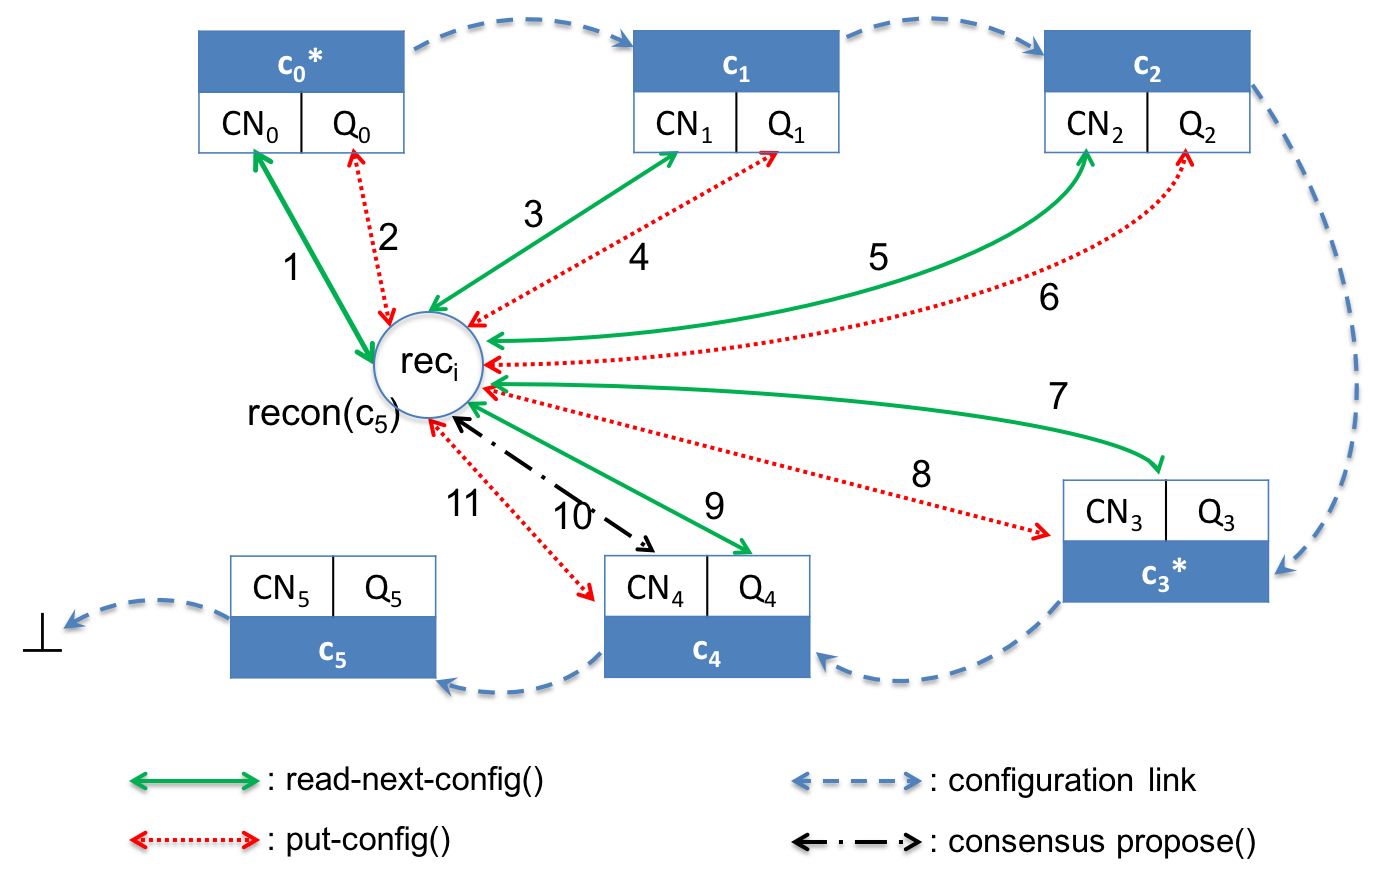
\includegraphics[width=0.5\textwidth]{ReconFig-v4.png}
			\caption{Illustration of an execution of the reconfiguration steps.}
			\label{fig:reconfig}
		\end{center}
		\vspace{-2.3em}
	\end{figure}
}

\sloppy$\act{finalize-config}(cseq)$:
Once the tag-value pair is transferred, in the last phase of the reconfiguration operation,  $rec_i$ executes %the procedure call 
$\act{finalize-config}(cseq)$, 
%during which, it 
to update the status of the last configuration in $cseq$, say $d = \config{\cseq{cseq[\nu]}}$, to $F$. 
%and writes to a quorum of the penultimate configuration of $cseq$, i.e., $cseq[\nu -1]$ and completes the reconfiguration operation.
The reconfigurer $rec_i$ informs a quorum of servers in the previous configuration $c=\config{\cseq{cseq[\nu-1]}}$, i.e.  in some $Q \in \quorums{c}$, 
about the change of status, by executing the $\act{put-config}(c, \tup{d,F})$ action. 

\myparagraph{Server Protocol.}
Each server  responds to requests from clients (Alg.~\ref{algo:server}). 
A server waits for \nnrev{five}{two} types of messages: {\sc read-config} and  {\sc write-config}.
% {\sc query}, {\sc query-tag}, and {\sc write} messages. 
When a {\sc read-config } message is received for a particular configuration $c_k$, then the server returns $nextC$ variables of the servers in $\servers{c_k}$. %\nn{[NN:again this notation]} 
A {\sc write-config} message attempts to update the $nextC$ variable of the server with a particular tuple $cfgT_{in}$.
A server changes the value of its local $nextC.cfg$ in two cases: (i) $nextC.cfg=\bot$, or (ii) $\status{nextC}= P$.

Fig.~\ref{fig:reconfig} 
%\nn{[NN: this is wrong numbering. probably has to do with the numbering of algorithms]} 
illustrates an example execution of a reconfiguration operation
$\act{recon}(c_5)$. %and the traversal of a concurrent write operation. 
In this example, the reconfigurer $rec_i$ goes through a number of configuration queries (\act{read-next-config})
before it reaches configuration $c_4$ in which a quorum of servers replies with $nextC.cfg=\bot$. 
There it proposes $c_5$ to the consensus object of $c_4$ ($\consensus{c_4}.propose(c_5)$ on arrow 10), and 
once $c_5$ is decided, $\act{recon}(c_5)$ completes after executing $\act{finalize-config}(c_5)$.



%\red{Recent reconfiguration attempts with some 
% configuration is are attempted to be added to the end of the list as the last recent link $c_{\nu}$ to $c$.  The status variable $status$ for such a configuration is set to $P$ in a quorum of servers.
%%
% A reconfig client $rc$, executing $recon(rc)$ executes three main steps. During the first step (  Line XXX $cseq \leftarrow read-config(cseq))$, $rc$ traverses the links of the reconfigurations successively discovering the new configuration from a current one by reading the $nextC$ variable  from a quorum of servers in the current configuration. Note the initial configuration is the final 
% configuration in $cseq$ such that its status is in $F$.
% }
%\blue{
%The reconfiguration protocol aims to install a new configuration and transfer the knowledge from previous configurations
%to the newly installed configuration. In particular, when a reconfiguration is invoked, the reconfigurer issues an 
%$\act{add-config}(c)$ action to the $\recBox$ attempting to add its proposed configuration to the configuration sequence
%stored in the $\recBox$. The $\recBox$ atomically appends its local configuration sequence and returns the appended 
%configuration sequence, $cseq$, to the reconfigurer. Notice that the newly added configuration $c$ appears as the last 
%element of the sequence $cseq[|cseq|]=\tup{c,P}$.
%%
%We assume a consensus service that can be executed by the members of a configuration. In each configuration
%$k$ we run a consensus instance to agree on the configuration id of $k+1$. The servers maintain a $cseq$ 
%array and are queried for the configuration identifier in a particular index.  
%}
%\paragraph{State Variables} Here we describe the state variables in the writers, readers and servers.
%
%\myemph{Servers}:~ $\tg{}\in\N \times\wSet,~v\in V$
%		%$cseq[~]$, array with elements in $\confSet\times\{F,P\}$ with members:
%		%	$cseq[i].conf\in\confSet$, the configuration identifier
%		%	 $cseq[i].status\in\{F,P\}$, the pending or finalized status 


%
%\begin{algorithm}[!ht]
%	\caption{$\rdIOA{\text{ReconBox}}{}$ Automaton: Signature of the ReconBox service} \label{ioa:reconbox-sig}
%	\begin{algorithmic}[2]
%		\begin{multicols}{2}{\small
%%				
%%				\State {\bf Data Types:}
%%				\State\T $\msgSet \subseteq \{\text{\sc{read},\sc{write}\}}\times\tup{\Nat\times\valSet}\times\Nat$
%%				
%%				\Statex
%%				
%				\Part{Signature}{ \label{line:reconbox-sig}
%				%	\State {\bf Input:}
%					\State\T $\act{add-config}(c), c\in \confSet$
%					\State\T $\act{read-config}$
%					\State\T $\act{finalize-config}(start, end)$, ~$start,end\in \N^+$
%					
%				%	\Statex
%					
%				%	\State {\bf Output:}
%					%\State\T $\act{add-config-ack}(cseq)$, $cseq[i]\in\confSet\times\{F,P\}, 0\leq i \leq |cseq|$
%					%\State\T $\act{read-config-ack}(cseq)$, ~$cseq[i]\in\confSet\times\{F,P\}, 0\leq i \leq |cseq|$
%					%\State\T $\act{finalize-config-ack}$ 
%	%				\State {\bf Internal:}
%				}\EndPart \label{line:reconbox-sig-end}
%		}\end{multicols}
%	\end{algorithmic}	
%\end{algorithm}


%Let the  $\act{recon}(c_5)$ operation be invoked by a reconfigurer $rec_i$. 
%%and the write operation by %$\act{read-next-config}(c_3)$ step executed by 
%%some writer $w$.
%During the first round of communication (arrow 1 in figure), $rec_i$ queries a quorum of servers in $c_0$ (noted by $Q_0$) and finds
%out $c_1$ as the next configuration (i.e. the link $c_0$ to $c_1$ in the global configuration sequence),
%via $\act{read-next-config}(c_0)$ 
%. %(arrow heads 1 and 2). 
%That is, at least a single server in the quorum $Q_0$ replied with $nextC$, where $nextC.cfg=c_1$ to $rec_i$.
%Next, in the second round of communication, $rec_i$ writes back $c_1$ to some 
%quorum in $c_0$ via the step $\act{put-config}(c_0, c_1)$ (see arrow 2).  In the subsequent steps $rec_i$ 
%communicates with configurations $c_1$, $c_2$ and $c_3$, in a similar manner like the above two communication rounds for $c_0$ (see arrows 3-8). 
%However,  in the first communication round with servers in  $c_4$, $rec_i$ discovers that all servers in a quorum of 
%servers in $c_4$ replied with 
%%the $nextC$ returned from
%$nextC$ such that $nextC.cfg=\bot$ (arrow 9). In other words, a link from $c_4$ to another configuration is not discovered by $rec_i$. As a result, 
%$rec_i$ proposes $c_5$ to the consensus object in $c_4$, i.e.,  it invokes $\consensus{c_4}.propose(c_5)$ (arrow 10) and 
%$\consensus{c_4}.propose(c_5)$ returns $c_5$, i.e., $c_5$ is decided as the next configuration after $c_4$. Next, $rec_i$ writes $c_5$ to a 
%quorum of servers in $c_4$ via the $\act{put-config}(c_4, c_5)$ (arrow 11), and completes the operation after executing $\act{finalize-config}(c_5)$. 
%Writer $w$  
%%happens to 
%starts its operation 
%%and the 
%with an initial guess of $cseq$ 
%%it starts with has 
%that contains $c_3$ as the last 
%configuration with 
%%its corresponding 
%a $status$ as $F$. With the two rounds of communication  (arrow heads a, b, c and d) with the servers in $c_3$,
%$w$ discovers $c_4$. However, similar communication rounds with the servers in $c_4$ returns $\bot$, i.e.,  $\act{read-next-config}(c_4)$ returns $\bot$.

%To install a new configuration the reconfigurer has to execute the following steps: (i) attempt to add the 
%new configuration, (ii) transfer the latest data to the new configuration, and (iii) mark the new configuration 
%as finalized. Below we describe each action separately: 
%\begin{itemize}
%	\item \myemph{add-config}: The \act{add-config}(c) action attempts to add the proposed configuration $c$ at 
%	the end of the current configuration sequence. In brief, a new configuration is added by following these steps:
%	(i) perform a read-config at a guessed configuration and by following the finalized configurations try to establish 
%	a sequence with a single finalized and a set of pending configs, (ii) propose $c$ by running consensus on the 
%	last discovered configuration (trying to establish the immediately next config), and (iii) once you receive the 
%	decided configuration propagate the new sequence to the latest config.
%\end{itemize}
%
%The read-config operation needs to have a mechanism to discover the latest finalized configuration. 
%Thus when we try to read the configuration sequence from 
%
%The reconfigurer finalizes the last configuration in its $cseq$ as this is the last configuration he added. 
%To do so he first sets the status of the last configuration, say $c$, to $F$ and propagates its local $cseq$ 
%to the following configurations in sequence: (i) contacts a quorum in $c$, and then (ii) contacts a quorum in 
%$cseq[\mu]$, where $\mu$ is the last finalized configuration of $cseq$ (before $c$). This way we ensure that



%\subsection{\ares{} over a Replicated Atomic Read/Write Object}
%\label{ssec:replicated} 

%To demonstrate that the reconfiguration service provides sufficient properties to implement 
%a reconfigurable atomic read/write object, we first present  an algorithm 
%where the distributed object is replicated among the set of servers. 
%The read and write operations (Algorithms \ref{algo:writer} and \ref{algo:reader}) are similar
%to the two phase classic algorithm of \cite{ABD96}, when they are not concurrent with a reconfiguration operation. 


\begin{algorithm*}[!ht]
	%\hrule \F
	\begin{algorithmic}[2]
		\begin{multicols}{2}{\small
				\Part{Write Operation}
				\State at each writer $w_i$ 
				%\State {\bf State Variables:}
				%\State  $\tg{},\tg{max}\in\N^+\times\wSet,~v\in V, terminate\in\{true,false\}$
				%\State  $cseq[~]$, array with elements in $\confSet\times\{F,P\}$ with members:
				%\State\T $cseq[i].conf\in\confSet$, the configuration identifier
				%\State\T $cseq[i].status\in\{F,P\}$, the pending or finalized status 
				%\State {\bf Initialization:} 
				%\State $\tg{}\gets \tup{0,w_i}$
				%\State $v \gets \bot$
				%\State $cseq[0] = \tup{c_0,F}, terminate={\bf false}$
				\State {\bf State Variables:}
				%\State  $\tg{}\in\N^+\times\wSet,~v\in V$
				\State  $cseq[] s.t. cseq[j]\in\confSet\times\{F,P\}$ with members:
				%\State\T $cseq[j].cfg\in\confSet$, the configuration identifier
				%\State\T $cseq[j].status\in\{F,P\}$, the configuration status 
				\State {\bf Initialization:} 
				\State $cseq[0] = \tup{c_0,F}$
				
				\Statex		
				
				\Operation{write}{$val$}, $val \in V$ 
				%\State $wCounter\gets wCounter+1$
				\State $cseq\gets$\act{read-config}($cseq$)  \label{line:writer:readconfig} %\Comment{Read the latest configuration sequence}
				\State $\mu\gets\max(\{i: cseq[i].status = F\})$ \label{line:writer:lastfin}
				\State $\nu\gets |cseq|$ 
				\For{$i=\mu:\nu$}
				\State $\tg{max} \gets \max(\config{cseq[i]}.\act{get-tag}(), \tg{max})$  \label{line:writer:max}
				\EndFor
				\State $\tup{\tg{},v} \gets \tup{ \tup{\tg{max}.ts+1, \wrt_i}, val}$ \label{line:writer:increment}
				\State $done \gets false$
				\While{{\bf not} $done$} \label{line:writer:whilebegin}
				\State $\config{cseq[\nu]}.$\act{put-data}$(\tup{\tg{},v})$ \label{line:writer:prop}
				\State $cseq\gets$\act{read-config}($cseq$)
				\If{$|cseq| = \nu$}
				\State $done \gets  true$
				\Else
				\State $\nu\gets |cseq|$ \label{line:writer:whileend}
				\EndIf
				\EndWhile
				\EndOperation
				\EndPart
				
				\Part{Read Operation}
				\State at each reader $\rdr_i$ 
				\State {\bf State Variables:}
				\State  $cseq[] s.t. cseq[j]\in\confSet\times\{F,P\}$ with members:
				%			\State\T $cseq[j].cfg\in\confSet$, the configuration identifier
				%			\State\T $cseq[j].status\in\{F,P\}$, the configuration status 
				\State {\bf Initialization:} 
				\State $cseq[0] = \tup{c_0,F}$
				
				\Statex
				
				\Operation{read}{ } 
				%\State $wCounter\gets wCounter+1$
				\State $cseq\gets$\act{read-config}($cseq$)  \label{line:reader:readconfig}%\Comment{Read the latest configuration sequence}
				\State $\mu\gets\max(\{j: cseq[j].status = F\})$ \label{line:reader:lastfin}
				\State $\nu\gets |cseq|$ 
				\For{$i=\mu:\nu$} \label{line:rw:getdata:start}
				\State $\tup{\tg{},v} \gets \max(\config{cseq[i]}.\act{get-data}(), \tup{\tg{},v})$ \label{line:reader:max}
				\EndFor \label{line:rw:getdata:end}
				\State $done\gets {\bf false}$
				\While{{\bf not} $done$}  \label{line:reader:whilebegin}
				\State $\config{cseq[\nu]}.\act{put-data}(\tup{\tg{},v})$ \label{line:reader:prop}
				\State $cseq\gets$\act{read-config}($cseq$)
				\If{$|cseq| = \nu$}
				\State $done \gets  true$
				\Else
				\State $\nu\gets |cseq|$ \label{line:reader:whileend}
				\EndIf
				\EndWhile
				\State {\bf return} $v$
				\EndOperation
				\EndPart
				
				%		\Procedure{get-tag}{$c$}
				%		%	\State {\bf send} $(\text{\act{query}},\rdr)$ to every server $s\in \bigcup_{cseq[i]}members(\qs_{cseq[i].conf})$
				%		\State {\bf send} $(\text{{\sc query-tag}})$ to each  $s\in \servers{c}$
				%		\State {\bf until}    $\exists \quo{}, \quo{}\in\quorums{c}$ s.t. 
				%		\State\TT$\wrtr_i$ receives $\tup{t_s,v_s}$ from $\forall s\in\quo{}$ 
				%		\State $t_{max} \gets \max(\{t_s : \wrtr_i \text{ received } \tup{t_s,v_s} \text{ from } s \})$
				%		\State {\bf return} $t_{max}$
				%		\EndProcedure
				%		
				%		\Statex				
				%		\Procedure{put-data}{$c, \tup{\tg{},v})$}
				%		\State {\bf send} $(\text{{\sc write}}, \tup{\tg{},v})$ to each $s \in \servers{c}$
				%		\State {\bf until} $\exists \quo,  \quo \in \quorums{c}$ s.t. $\wrtr_i$ receives {\sc ack} from $\forall s\in\quo{}$
				%		\EndProcedure
				%		
				%		
				%		\Statex
				
				%		\Procedure{read-config}{$seq$}
				%		\State $\mu = \max(\{j: seq[j].status = F\})$	\label{line:readconfig:final}
				%		%\State $\nu = |cseq|$
				%		\State $c \gets seq[\mu].cfg$
				%		%\State {\bf send} $(\text{{\sc read-config}}, recon_i)$ to each   $s\in \bigcup_{\mu \leq i \leq \nu} \servers{currCfg}$
				%		\While{$c \neq \bot$}
				%		%\State {\bf send} $(\text{\act{read-config}}, recon_i)$ to each $s\in \servers{c}$
				%		%\State {\bf until}  $\forall j,  \mu \leq j\leq \nu$  $\wedge$  
				%		%$\exists\quo{},  \quo{} \in \quorums{cseq[j].cfg}$ s.t. $ \forall s\in\quo{},  recon_i$  receives $cseq_s$ from $s$ 
				%		%\State {\bf until} $\exists\quo{},  \quo{}\in\quorums{c}$ s.t. $\forall s\in\quo{}, recon_i$  receives $nextC_s$ from $s$
				%		%\State $ell \gets \max_{cseq'\text{ received }}(|cseq'|)$
				%		\State $nextC \gets$\act{get-next-config}$(c)$ 
				%		\If{$nextC.cfg\neq\bot$} 
				%		\State $\mu\gets \mu+1$				\label{line:readconfig:increment}
				%		\State $seq[\mu] \gets nextC$	\label{line:readconfig:assign}
				%		\State \act{put-config}$(seq[\mu-1].cfg, seq[\mu])$
				%		\State $c \gets seq[\mu].cfg$
				%		\Else
				%		\State $c \gets \bot$
				%		\EndIf
				%		\EndWhile
				%		\State {\bf return} $seq$
				%		\EndProcedure
				%		
				%		\Statex		
				%		
				%		\Procedure{get-next-config}{$c$}
				%		\State {\bf send} $(\text{{\sc read-config}})$ to each $s\in \servers{c}$
				%		\State {\bf until} $\exists\quo{},  \quo{}\in\quorums{c}$ s.t. $\wrtr_i$ receives $nextC_s$, $\forall s\in\quo{}$
				%		\If{$\exists s\in \quo{}\text{ s.t. } nextC_s.cfg\neq\bot$} 
				%		\State {\bf return} $nextC_s$
				%		\Else
				%		\State {\bf return} $\bot$
				%		\EndIf 
				%		\EndProcedure
				%		
				%		\Statex
				%		
				%		\Procedure{put-config}{$c, cfgPtr)$}
				%		\State {\bf send} $(\text{{\sc write-config}}, cfgPtr)$ to each $s\in \servers{c}$
				%		\State {\bf until} $\exists\quo{},  \quo{}\in\quorums{c}$ s.t. $\wrtr_i$ receives {\sc ack} from $\forall s\in\quo{}$
				%		\EndProcedure
		}\end{multicols}	
	\end{algorithmic}
	%\hrule \B
	\caption{Write and Read protocols at the clients for \ares.}
	\label{algo:writer}
	\vspace{-1em}
\end{algorithm*}
\subsection{Implementation of Read and Write operations.}
The read and write operations in \ares{} are expressed in terms of the DAP primitives  (see 
Section \ref{ssec:dap}). 
%A read  consists of  an execution of  $\act{get-data}$ primitive followed by a $\act{put-data}$ primitive,
%while a write consists of calls to $\act{get-tag}$ and  $\act{put-data}$ primitives. 
This provides the flexibility to \ares{} to use different implementation of DAP primitives in different configurations, without changing the basic structure of  \ares{}. 
At a high-level, a \act{write} (or \act{read})  operation is executed where the client: $(i)$ obtains the \textit{latest configuration sequence} by using the 
$\act{read-config}$ action of the reconfiguration service, $(ii)$ queries  the configurations, in $cseq$, starting from the last finalized configuration
to the end of the discovered configuration 
sequence, for the latest $\tup{tag,value}$ pair with a help of $\act{get-tag}$ (or $\act{get-data}$) operation \nn{as specified for each configuration}, and 
$(iii)$ repeatedly propagates  a new $\tup{tag', value'}$ pair (the largest $\tup{tag,value}$ pair)   with $\act{put-data}$ in the last configuration of its local sequence, until no additional configuration is observed. 
%Now
%{\sc get} and {\sc put} primitives 
%we  describe the execution 
In more detail, the algorithm of a  read or write operation $\pi$ is as follows (see Alg.~\ref{algo:writer}): 
%The server keeps a passive behavior and replies to any message it receives. 


%Here we present the read and write operations in more detail. 
%As we presented in Section \ref{sec:primitives}, for an algorithm to 
%preserve atomicity it needs to satisfy some properties on the 
%implementation of its {\sc get} and {\sc put} primitives. 

%Those primitives are implemented in our replication algorithm as follows:
%\begin{itemize}
%	\item {\sc get-tag}$(c)$: Send {\sc query-tag} messages to all the servers in $\servers{c}$ and wait 
%	for each server $s$ in a quorum $Q\in\quorums{q}$ to reply with its local $\tg{s}$. Find and return the 
%	maximum of those tags. 
%	\item {\sc get-data}$(c)$: Send {\sc query} messages to all the servers in $\servers{c}$ and wait 
%	for each server $s$ in a quorum $Q\in\quorums{q}$ to reply with its local $\tup{\tg{s}, v_s}$ pair. 
%	Find the maximum of those tags, say $\tg{s'}$, and return the pair received by $s'$, $\tup{\tg{s'},v_{s'}}$.
%	\item {\sc put-data}$(c, \tup{\tg{},v})$: Send {\sc write-tag} messages, along with the  $\tup{\tg{},v}$ pair, 
%	to all the servers in $\servers{c}$ and wait for each server $s$ in a quorum $Q\in\quorums{q}$ to reply with an {\sc ack}. 
%\end{itemize}


A write (or read) operation is invoked at a client  $\pr$ when line~Alg.~\ref{algo:writer}:\ref{line:writer:readconfig} %for the writer  
(resp. line~Alg.~\ref{algo:writer}:\ref{line:reader:readconfig}) is executed.  
%for reader),
At first, $\pr$ issues a $\act{read-config}$ action to obtain the latest 
introduced configuration in $\gseq$, in both operations. 
%Note that each process contains a state 
%variable $cseq$ which initially contains the initial configuration $\tup{c_0,F}$. 
%Starting with a guess, $cseq$, for the latest global configuration sequence,
%As shown in the reconfiguration service, 
%process $\pr$ queries a quorum in each configuration $\config{cseq[i]}$, for $\max(j:\status{cseq[j]}=F)\leq i \leq |cseq|$,
%to discover newly introduced and/or newly finalized configurations, during the $\act{read-config}$ action. 

%We assume that each configuration has enough active servers to allow 
%$\pr$ to make progress	even when some configuration is has been replaced 
%by a newer configuration. 
%In case a system wants to garbage collect or decommission inactive servers,
%then a service similar to DNS can be used to provide an estimate of 
%the latest finalized configuration. Notice that such a service would affect 
%the liveness and not the safety of our current implementation so we do 
%not get into details on how such a service can be implemented in this paper. 

\nn{If $\op$ is a \act{write} %(resp. Alg.~\ref{algo:writer}:\ref{line:reader:lastfin} if $\op$ is a  read), 
	$\pr$ detects the last finalized entry in $cseq$, 
	say $\mu$, and performs a $cseq[j].conf.\act{get-tag}()$ action,
	for $\mu\leq j\leq|cseq|$ (line Alg.~\ref{algo:writer}:\ref{line:writer:lastfin}). Then $\pr$ discovers the
	\textit{maximum tag} among all the returned tags ($\tg{max}$),
	and it increments the maximum tag discovered 
	(by incrementing the integer part of $\tg{max}$), generating a new tag, say $\tg{new}$. It assigns 
	$\tup{\tg{}, v}$ to $\tup{\tg{new}, val}$, where $val$ is the
	value he wants to write (Line Alg.~\ref{algo:writer}:\ref{line:writer:increment}).}

\nn{
if $\op$ is a \act{read}, 
$\pr$ detects the last finalized entry in $cseq$, 
say $\mu$, and performs a  $cseq[j].conf.\act{get-data}()$ action, 
for $\mu\leq j\leq|cseq|$ (line Alg.~\ref{algo:writer}:\ref{line:reader:lastfin}). Then $\pr$ discovers the
\textit{maximum tag-value} pair ($\tup{\tg{max},v_{max}}$) among the replies, 
and assigns $\tup{\tg{}, v}$ to $\tup{\tg{max},v_{max}}$.}

%In lines Alg.~\ref{algo:writer}:\ref{line:writer:lastfin} if $\op$ is a write (resp. Alg.~\ref{algo:writer}:\ref{line:reader:lastfin} if $\op$ is a  read), 
% $\pr$ detects the last finalized entry in $cseq$, 
%say $\mu$, and performs a $cseq[j].conf.\act{get-tag}()$ action if $\op$ is a \act{write}, or $cseq[j].conf.\act{get-data}()$ action if $\op$ is a \act{read}, 
%for $\mu\leq j\leq|cseq|$. Then $\pr$ discovers the
%maximum tag among all the returned tags ($\tg{max}$) or tag-value pairs ($\tup{\tg{max},v_{max}}$) respectively.
%%sends \textit{query} messages to all the members of each configuration $cseq[j].conf$, for $\mu\leq j\leq|cseq|$.
%%Notice that any configuration $cseq[j].cfg$,  for $\mu< j\leq|cseq|$, is in a pending state and thus $cseq[j].status = P$.
%%When the client receives replies from a quorum in each configuration $cseq[j].cfg$, it discovers the maximum 
%%$\tup{\tg{max},v_{max}}$ among those replies (Lines A\ref{algo:writer}:\ref{line:writer:max} and A\ref{algo:reader}:\ref{line:reader:max}). 
%If $\op$ is a \act{write}, $\pr$ increments the maximum tag discovered 
%(by incrementing the integer part of $\tg{max}$), generates a new tag, say $\tg{new}$, and assigns 
%$\tup{\tg{}, v}$ to $\tup{\tg{new}, val}$, where $val$ is the
%value he wants to write (Line Alg.~\ref{algo:writer}:\ref{line:writer:increment}). If $\op$ is a \act{read}, then $\pr$ assigns 
%$\tup{\tg{}, v}$ to $\tup{\tg{max},v_{max}}$, i.e.,  the maximum discovered tag-value pair.
%

Once specifying the $\tup{\tg{}, v}$ to be propagated, both reads and writes 
% if $\op$ is a read, $\pr$ 
 %does the following until no new configuration is discovered: (i) 
execute the $\config{cseq[\nu]}.\act{put-data}(\tup{\tg{}, v})$ action, where $\nu=|cseq|$, 
%to a quorum in the last configuration in $cseq$, 
followed by executing  $\act{read-config}$ action, to examine whether new configurations were 
introduced in $\gseq$. The repeat these steps until no new configuration is discovered (lines  Alg.~\ref{algo:writer}:\ref{line:writer:whilebegin}--\ref{line:writer:whileend},
or lines  Alg.~\ref{algo:writer}:\ref{line:reader:whilebegin}--\ref{line:reader:whileend}).
%retrieving a config
Let $cseq'$ be the sequence returned by the $\act{read-config}$ action. 
If $|cseq'| = |cseq|$ then no new configuration is introduced, and
the read/write operation terminates; otherwise, $\pr$ sets $cseq$ to $cseq'$ and repeats the two actions. 
Note,  in an execution of  \ares,  two consecutive $\act{read-config}$ 
operations that return $cseq'$ and $cseq''$ respectively must hold that $cseq'$ is a prefix of $cseq''$,
and hence $|cseq'|=|cseq''|$ only if $cseq' = cseq''$.  Finally, if $\pi$ is a read operation the value with the highest
tag discovered is returned to the client.

\nnfix{\myparagraph{Discussion} \ares{} shares similarities with previous algorithms like RAMBO \cite{GLS03} and 
	the framework  in \cite{spiegelman:DISC:2017}. The reconfiguration technique used in \ares{} ensures the prefix property 
	on the configuration sequence (resembling a blockchain data structure \cite{N08bitcoin}) while the array structure in RAMBO allowed 
	nodes to maintain an incomplete reconfiguration history. 
	%While in RAMBO recon operation needed to write in both the old and the new configurations due to the possible non-continuity of the 
	%known configurations in the config array, in ARES the prefix property of the configuration sequence 
	%allows each recon operation to write only to the latest configuration it discovered. 
	On the other hand, the DAP usage, 
	%enables \ares{} to be oblivious on the underlying atomic memory implementation in each configuration. This 
	exploits a different viewpoint compared to \cite{spiegelman:DISC:2017}, allowing implementations of 
	atomic read/write registers without relying on strong objects, like ranked registers \cite{GD05}.	
	%	where the authors focus to provide a general framework 
	%	for reconfigurations that led to the use of read-write-modify objects, like ranked registers \cite{GD05},
	%	for the implementation of linearizable read/write objects.  
} 

%\vspace{-0.25em}
%\label{sec:correct}
%\remove{We proceed by first introducing some definitions and notation, then by presenting some properties that are satisfied 
by the reconfiguration service in any execution, and then we show that given these properties our algorithm satisfies 
the safety (atomicity) conditions. 
%Due to space limitations the proofs of the main statements are omitted and can be found in \cite{ARES:Arxiv:2018}.
}

\remove{
\myparagraph{Notations and definitions.}
For a server $s$, we use the notation $\atT{s.var}{\state}$ to refer to the value of the state variable $var$, in $s$, at a state $\state$ of an  execution $\EX$. 
If server  $s$ crashes at a state $\state_f$ in an execution $\EX$ then $\atT{s.var}{\state}\triangleq\atT{s.var}{\state_f}$ for any state variable $var$ and for 
any state $\state$ that appears after $\state_f$ in $\EX$. 
%refers to the value of $v$ at $s$ at the state just before crashes. In other words, $\atT{s.v}{T}  \triangleq \atT{s.v}{\hat{T}}$, where $\hat{T}$ is the latest point in the execution, such that, $(a)$ $\hat{T} \leq T$ and $(b)$ $s$ is non-faulty.
 }
 
 \remove{
\begin{definition}[Tag of a configuration]  Let  $c \in \mathcal{C}$ be a configuration, $\state$ be a state in some execution $\EX$ then 
we define the tag of $c$ at state $\state$ as  
$ \atT{tag(c)}{\state} \triangleq \min_{Q \in \quorums{c}} \max_{s \in Q}~\atT{(s.tag}{\state}).$
We  drop the suffix $|_\state$, and simply denote as $tag(c)$,  when the state  is clear from the context.
\end{definition}

\begin{definition}
Let $\sigma$ be any point in an execution of \ares{} and suppose we use the notation $\cvec{\pr}{\state}$ for $ \atT{\pr.cseq}{\state}$,  i.e., the $cseq$ variable at process $p$ at the state $\state$. %be the value of a configuration sequence vector at a process $\pr$ at some state  $\st$ in an execution $\EX$. 
Then we define as $ \mu(\cvec{\pr}{\state})  \triangleq  \max\{ i : \cvec{\pr}{\state}[i].status = F\}$ 
and $ \nu(\cvec{\pr}{\state}) \triangleq |\cvec{\pr}{\state}|$, where $|\cvec{\pr}{\state}|$ is the length of the  configuration vector 
$\cvec{\pr}{\state}$. % that are not equal to $\bot$.  
\end{definition}

\begin{definition} [Prefix order]
Let $\mathbf{x}$ and $\mathbf{y}$ be any two configuration sequences. We say that $\mathbf{x}$ is a prefix of $\mathbf{y}$, denoted by 
$\mathbf{x} \preceq_p  \mathbf{y}$, if $\config{\mathbf{x}[j]}=\config{\mathbf{y}[j]}$, for all $j$ such that $\mathbf{x}[j]\neq\bot$.
\end{definition}

%In this section we analyze the properties that we can achieve through our reconfiguration algorithm. 
The first lemma shows that any two configuration sequences have the same configuration identifiers
in the same indexes. 

\begin{lemma}
\label{lem:consconf}
	For any reconfigurer $r$ that invokes an $\act{reconfig}(c)$ action in an execution $\EX$ 
	of the algorithm, If $r$ chooses to install $c$ in index $k$ of its local $r.cseq$ vector, then $r$ invokes 
	the $Cons[k-1].propose(c)$ instance over configuration $r.cseq[k-1].cfg$.
\end{lemma}

\begin{proof}
	It follows directly from the algorithm. 
\end{proof}

\begin{lemma}
	\label{lem:server:monotonic}
	If a server $s$ sets $s.nextC$ to $\tup{c,F}$ at some state $\st$ in an execution $\EX$ 
	of the algorithm, then $s.nextC = \tup{c,F}$ for any state $\st'$ that appears after $\st$ in 
	$\EX$.
\end{lemma}

\begin{proof}
	Notice that a server $s$ updates the $s.nextC$ variable for some specific configuration $c_k$ 
	in a state $st$ if: (i) $s$ did not receive any value for $c_k$ before (and thus $nextC=\bot$), or (ii) $s$ 
	received a tuple $\tup{c,P}$ and before $\st$ received the tuple $\tup{c',F}$. By Observation \ref{obs:consensus}
	$c=c'$ as $s$ updates the $s.nextC$ of the same configuration $c_k$. Once the tuple becomes equal to 
	$\tup{c,F}$ then $s$ does not satisfy the update condition for $c_k$, and hence in any state $\st'$ after $\st$
	it does not change $\tup{c,F}$.
\end{proof}

\begin{lemma}[Configuration Uniqueness]
\label{lem:unique}

	%Let $\st_1$ and $\st_2$ be any two states of an execution $\EX$ of the algorithm,
	%and $\pr, q$ two participating processes. 
	%be the state after the response action of an operation $\op_1$ from process $p$,
	%and $\st_2$ be the state after the first $\act{read-config}$ call of an operation $\op_2$ from $q$.
	For any processes $\pr, q\in \idSet$ and any states $\st_1, \st_2$ in an execution $\EX$, it must hold that 
	$\config{\cvec{\pr}{\st_1}[i]}=\config{\cvec{q}{\st_2}[i]}$,  $\forall i$ s.t. 
	$\config{\cvec{\pr}{\st_1}[i]},\config{\cvec{q}{\st_2}[i]}\neq \bot$.
\end{lemma}

\begin{proof}
	The lemma holds trivially for $\config{\cvec{\pr}{\st_1}[0]}=\config{\cvec{q}{\st_2}[0]}=c_0$. 
	So in the rest of the proof we focus in the case where $i > 0$. Let us assume 
	w.l.o.g. that $\st_1$ appears before $\st_2$ in $\EX$.
	
	According to our algorithm a process $\pr$ sets $\pr.cseq[i].cfg$ to a configuration 
	identifier $c$ in two cases: (i) either it received $c$ as the result of the consensus 
	instance in configuration $\pr.cseq[i-1].cfg$, or (ii) $\pr$ receives $\config{s.nextC} = c$ from 
	a server $s\in\servers{\config{\pr.cseq[i-1]}}$. Note here that (i) is possible only 
	when $\pr$ is a reconfigurer and attempts to install a new configuration. On the 
	other hand (ii) may be executed by any process in any operation that invokes the 
	$\act{read-config}$ action. We are going 
	to proof this lemma by induction on the configuration index. 
	

	\emph{Base case:} The base case of the lemma is when $i=1$. 
	Let us first assume that $p$ and $q$ receive $c_p$ and $c_q$, as the result of the consensus instance at $\pr.cseq[0].cfg$
	and $q.cseq[0].cfg$ respectively. By Lemma \ref{lem:consconf}, since both processes want to install a configuration 
	in $i=1$, then they have to run $Cons[0]$ instance over the configuration stored in their local $cseq[0].cfg$ variable. 
	Since $\pr.cseq[0].cfg=q.cseq[0].cfg=c_0$ then 
	both $Cons[0]$ instances run over the same configuration $c_0$ and according to Observation \ref{obs:consensus}  
	return the same value, say $c_1$. Hence $c_p=c_q=c_1$ and $\pr.cseq[1].cfg=q.cseq[1].cfg=c_1$.
	 
	 Let us examine the case now where $p$ or $q$ 
	assign a configuration $c$ they received from some server $s\in\servers{c_0}$. According to the
	algorithm only the configuration that has been decided by the consensus instance on 
	$c_0$ is propagated to the servers in $\servers{c_0}$. If $c_1$ is the decided configuration, then 
	$\forall s\in\servers{c_0}$ such that $s.nextC(c_0)\neq\bot$, it holds that $s.nextC(C_0) = \tup{c_1,*}$.
	So if $p$ or $q$ set $\pr.cseq[1].cfg$ or $q.cseq[1].cfg$ to some received configuration, then 
	$\pr.cseq[1].cfg = q.cseq[1].cfg = c_1$ in this case as well. 
	
     \emph{Hypothesis:} We assume  that 
	$\cvec{\pr}{\st_1}[k]=\cvec{q}{\st_2}[k]$  for some $k$, $k \geq 1$.
	
	%\noindent{\bf Induction Hypothesis:} 
	\emph{Induction Step:}  We need to show that the lemma holds for $i=k+1$.
	If both processes retrieve $\config{\pr.cseq[k+1]}$ and $\config{q.cseq[k+1]}$ through consensus, 
	then both $\pr$ and $q$ run consensus
	over the previous configuration. Since according to our hypothesis 
	$\cvec{\pr}{\st_1}[k]=\cvec{q}{\st_2}[k]$ then both process will receive the same
	decided value, say $c_{k+1}$, and hence $\pr.cseq[k+1].cfg=q.cseq[k+1].cfg=c_{k+1}$. Similar to the base case,
	a server in $\servers{c_k}$ only receives the configuration $c_{k+1}$ decided by the consensus instance run over $c_k$. 
	So processes 
	$\pr$ and $q$ can only receive $c_{k+1}$ from some server in $\servers{c_k}$ 
	%even if the processes update their $\pr.cseq[k+1].cfg$ or $q.cseq[k+1].cfg$ with a received 
	%configuration that will be equal to 
	so they can only assign $\pr.cseq[k+1].cfg=q.cseq[k+1].cfg=c_{k+1}$ at Line \ref{algo:reconfigurer}:\ref{line:readconfig:assign}.
	That completes the proof. 
\end{proof}


Lemma \ref{lem:unique} showed that any two operations store the same
configuration in any cell $k$ of their $cseq$ variable. It is not known however 
if the two processes discover the same number of configuration ids. In the following
lemmas we will show that if a process learns about a configuration in a cell $k$ 
then it also learns about all configuration ids for every index $i$, such that $0\leq i\leq k-1$.

\begin{lemma}
\label{lem:confmonotonic}
	In any execution $\EX$ of the algorithm , If for any process $\pr\in\idSet$, $\cvec{\pr}{\st}[i]\neq\bot$ in some state $\st$ in $\EX$,
	then $\cvec{\pr}{\st'}[i]\neq\bot$ in any state $\st'$ that appears after $\st$ in $\EX$. 
\end{lemma}

\begin{proof}
	A value is assigned to $\cvec{\pr}{*}[i]$ either after the invocation of a consensus instance, or while executing
	the $\act{read-config}$ action. Since any configuration proposed for installation cannot be $\bot$ (A\ref{algo:reconfigurer}:\ref{line:install:valid}), 
	and since there is at least one configuration proposed in the consensus instance (the one from $\pr$), then by the validity of the consensus
	service the decision will be a configuration $c\neq\bot$. Thus, in this case $\cvec{\pr}{*}[i]$ cannot be $\bot$.
	Also in the $\act{read-config}$ procedure, $\cvec{\pr}{*}[i]$ is assigned to a value different than $\bot$ according
	to Line A\ref{algo:reconfigurer}:L\ref{line:readconfig:assign}. Hence, if $\cvec{\pr}{\st}[i]\neq\bot$ at state $\st$ 
	then it cannot become $\bot$ in any state $\st'$ after $\st$ in execution $\EX$.
\end{proof}


\begin{lemma}
\label{lem:nogaps}
	Let $\st_1$ be some state in an execution $\EX$ of the algorithm. Then for any 
	process $\pr$, if $k = max\{i: \cvec{\pr}{\st_1}[i]\neq \bot\}$, then 
	$\cvec{\pr}{\st_1}[j]\neq \bot$, for $0\leq j < k$.
\end{lemma}
\begin{proof}
	Let us assume to derive contradiction that there exists $j < k$ such that 
	$\cvec{\pr}{\st_1}[j]=\bot$ and $\cvec{\pr}{\st_1}[j+1]\neq\bot$.
	Suppose w.l.o.g. that $j = k-1$ and that $\st_1$ is the state immediately 
	after the assignment of a value to $\cvec{\pr}{\st_1}[k]$, say $c_k$. 
	Since $\cvec{\pr}{\st_1}[k]\neq\bot$, then $\pr$ assigned $c_k$ to $\cvec{\pr}{\st_1}[k]$ 
	in one of the following cases: 
	(i) $c_k$ was the result of the consensus instance, or
	(ii) $\pr$ received $c_k$ from a server during a $\act{read-config}$ action.
	The first case is trivially impossible as according to Lemma \ref{lem:consconf} 
	$\pr$ decides for $k$ when it runs consensus over configuration $\config{\cvec{\pr}{\st_1}[k-1]}$. 
	Since this is equal to $\bot$, then we cannot run consensus over a non-existent set of 
	processes. 	In the second case, $\pr$ assigns $\cvec{\pr}{\st_1}[k] = c_k$  in Line A\ref{algo:parser}:\ref{line:readconfig:assign}.
	The value $c_k$ was however obtained when $\pr$ invoked $\act{get-next-config}$ on 
	configuration $\config{\cvec{\pr}{\st_1}[k-1]}$. In that action, $\pr$ sends {\sc read-config}
	messages to the servers in $\servers{\config{\cvec{\pr}{\st_1}[k-1]}}$ and waits until a quorum 
	of servers replies. Since we assigned $\cvec{\pr}{\st_1}[k] = c_k$ it means that $\act{get-next-config}$
	terminated at some state $\st'$ before $\st_1$ in $\EX$, and thus: 
	(a) a quorum of servers in $\servers{\config{\cvec{\pr}{\st'}[k-1]}}$
	replied, and (b) there exists a server $s$ among those that replied with $c_k$. 
	According to our assumption however, $\cvec{\pr}{\st_1}[k-1] = \bot$ at $\st_1$. 
	So if state $\st'$ is before $\st_1$ in $\EX$, %is the state after the response step of $\act{get-next-config}$, 
	then by Lemma \ref{lem:confmonotonic}, it follows that $\cvec{\pr}{\st'}[k-1] = \bot$. This however 
	implies that $\pr$ communicated with an empty configuration, and thus no server replied to $\pr$. 
	This however contradicts the assumption that a server replied with $c_k$ to $\pr$. 
	
	Since any process traverses the configuration sequence starting from the initial 
	configuration $c_0$, then with a simple induction we can show that 
	$\cvec{\pr}{\st_1}[j]\neq \bot$, for $0\leq j\leq k$.
\end{proof}

We can now move to an important lemma that shows that any \act{read-config} action 
returns an extension of the configuration sequence returned by any previous \act{read-config} action. 
First, we show that the last finalized configuration observed by any \act{read-config} action is at least as 
recent as the finalized configuration observed by any subsequent \act{read-config} action. 
%Using this lemma we will then show that when 

\begin{lemma}
	\label{lem:config:propagation}
	If at a state $\st$ of an execution $\EX$ of the algorithm, if $\mu(\cvec{\pr}{\st}) = k$ % = \max\{i: \cvec{\pr}{\st}[i]\neq\bot\}$
	for some process $\pr$, then for any element $0\leq j < k$, $\exists Q\in \quorums{\config{\cvec{\pr}{\st}[j]}}$
	such that $\forall s\in Q, s.nextC(\config{\cvec{\pr}{\st}[j]})= \cvec{\pr}{\st}[j+1]$. 
\end{lemma}
\begin{proof}
	This lemma follows directly from the algorithm. Notice that whenever a process assigns a value to 
	an element of its local configuration (Lines  A\ref{algo:parser}:\ref{line:readconfig:assign} and 
	A\ref{algo:reconfigurer}:\ref{line:addconfig:assign}), it then propagates this value to a quorum of the 
	previous configuration (Lines  A\ref{algo:parser}:\ref{line:readconfig:put} and 
	A\ref{algo:reconfigurer}:\ref{line:addconfig:put}). So if a process $\pr$ assigned $c_j$ to an 
	element $\cvec{\pr}{\st'}[j]$ in some state $\st'$ in $\EX$, then $\pr$ may assign a value 
	to the $j+1$ element of $\cvec{\pr}{\st''}[j+1]$ only after $\act{put-config}(\config{\cvec{\pr}{\st'}[j-1]},\cvec{\pr}{\st'}[j])$
	occurs. During $\act{put-config}$ action, $\pr$ propagates $\cvec{\pr}{\st'}[j]$ in a quorum 
	$Q\in\quorums{\config{\cvec{\pr}{\st'}[j-1]}}$. Hence, if $\cvec{\pr}{\st}[k]\neq\bot$, then $\pr$ 
	propagated each $\cvec{\pr}{\st'}[j]$, for $0<j\leq k$ to a quorum of servers $Q\in\quorums{\config{\cvec{\pr}{\st'}[j-1]}}$.
	And this completes the proof. 
%	
%	Let examine a single element $\cvec{\pr}{\st'}[j]$ that is added in the configuration vector at some state $\st'$ 
%	that appears before $\st$ in $\EX$. Whenever a configuration is assigned a process $\pr$ invokes $\act{put-config}$
%	action before adding the next configuration. According to this action, the process sends the discovered configuration
%	and sends it to a quorum of servers. As this process is repeated for every element inserted then the lemma follows. 
\end{proof}


\begin{lemma}[Configuration Prefix]
	\label{lem:prefix}
Let $\op_1$ and $\op_2$ two 
%read/write/install operations 
completed \act{read-config} actions invoked by processes $\pr_1, \pr_2\in\idSet$ 
respectively, such that $\op_1\bef\op_2$ in an execution $\EX$. Let $\st_1$ be the state after the response 
step of $\op_1$ and $\st_2$ the state after the response step 
%termination of the first $\act{read-config}$ 
of $\op_2$. Then 
$\cvec{\pr_1}{\st_1}\preceq_p\cvec{\pr_2}{\st_2}$.
\end{lemma}

\begin{proof}
	Let $\nu_1 = \nu(\cvec{\pr_1}{\st_1})$ and $\nu_2 = \nu(\cvec{\pr_2}{\st_2})$.
	By Lemma \ref{lem:unique} for any $i$ such that $\cvec{\pr_1}{\st_1}[i]\neq\bot$ and 
	$\cvec{\pr_2}{\st_2}[i]\neq\bot$, then $\config{\cvec{\pr_1}{\st_1}[i]}=\config{\cvec{\pr_2}{\st_2}[i]}$.
	Also from Lemma \ref{lem:nogaps} we know that for $0\leq j\leq \nu_1, \cvec{\pr_1}{\st_1}[j] \neq \bot$, 
	and $0\leq j\leq \nu_2, \cvec{\pr_2}{\st_2}[j] \neq \bot$. So if we can show that $\nu_1\leq \nu_2$ then the lemma follows. 
	
	Let $\mu = \mu(\cvec{\pr_2}{\st'})$ %, or simply $\mu$, 
	be the last finalized element which $\pr_2$ established in the beginning of 
	the $\act{read-config}$ action $\op_2$ (Line A\ref{algo:reconfigurer}:\ref{line:readconfig:final}) at some state $\st'$ before $\st_2$. 
	It is easy to see that $\mu\leq \nu_2$. If $\nu_1 \leq \mu$ then $\nu_1\leq \nu_2$ and 
	the lemma follows. Thus, it remains
	to examine the case where $\mu < \nu_1$. Notice that since $\op_1\bef\op_2$ then $\st_1$ appears before 
	$\st'$ in execution $\EX$. By Lemma \ref{lem:config:propagation}, we know that by $\st_1$, 
	%in all the configurations $\cvec{\pr_1}{\st_1}[j]$, for $0\leq j < \nu_1$,  
	$\exists Q\in\quorums{\config{\cvec{\pr_1}{\st_1}[j]}}$, for $0\leq j < \nu_1$,   such that 
	$\forall s\in Q, s.nextC = \cvec{\pr_1}{\st_1}[j+1]$. Since $\mu < \nu_1$, then it must be the case 
	that $\exists Q\in \quorums{\config{\cvec{\pr_1}{\st_1}[\mu]}}$ such that $\forall s\in Q, s.nextC = \cvec{\pr_1}{\st_1}[\mu+1]$.
	But by Lemma \ref{lem:unique}, we know that $\config{\cvec{\pr_1}{\st_1}[\mu]}= \config{\cvec{\pr_2}{\st'}[\mu]}$. 
	Let $Q'$ be the quorum that replies to the $\act{read-next-config}$ occurred in $\pr_2$, on configuration  $\config{\cvec{\pr_2}{\st'}[\mu]}$.
	By definition $Q\cap Q'\neq \emptyset$, thus there is a server $s\in Q\cap Q'$ that sends $s.nextC = \cvec{\pr_1}{\st_1}[\mu+1]$
	to $\pr_2$ during $\op_2$. Since $\cvec{\pr_1}{\st_1}[\mu+1]\neq\bot$ then $\pr_2$ assigns $\cvec{\pr_2}{*}[\mu+1]=\cvec{\pr_1}{\st_1}[\mu+1]$, and 
	repeats the process in the configuration $\config{\cvec{\pr_2}{*}[\mu+1]}$. Since every configuration $\config{\cvec{\pr_1}{\st_1}[j]}$, 
		for $\mu\leq j<\nu_1$, has a quorum of servers with $s.nextC$, then by a simple induction it can be shown that the process will 
		be repeated for at least $\nu_1-\mu$ iterations, and  every configuration
		$\cvec{\pr_2}{\st''}[j]=\cvec{\pr_1}{\st_1}[j]$, at some state $\st''$ before $\st_2$. 
		Thus, $\cvec{\pr_2}{\st_2}[j]=\cvec{\pr_1}{\st_1}[j]$, for $0\leq j\leq \nu_1$. Hence $\nu_1\leq\nu_2$ and the lemma follows in this case as well. 
\end{proof}

Thus far we focused on the configuration member of each element in $cseq$. As operations do get in account
the \emph{status} of a configuration, i.e. $P$ or $F$, in the next lemma we will examine the relationship of 
the last finalized configuration as detected by two operations. First we present a lemma that shows the 
monotonicity of the finalized configurations.

\begin{lemma}
	\label{lem:final:monotonic}
	Let $\st$ and $\st'$ two states in an execution $\EX$ such that $\st$ appears before $\st'$ in $\EX$.
 	Then for any process $\pr$ must hold that $\mu(\cvec{\pr}{\st})\leq \mu(\cvec{\pr}{\st'})$.  %\red{must refer to a read-config}
\end{lemma}

\begin{proof}
	This lemma follows from the fact that if a configuration $k$ is such that 
	$\status{\cvec{\pr}{\st}[k]}=F$ at a state $\st$, then $\pr$ will start any 
	future $\act{read-config}$ action from a configuration $\config{\cvec{\pr}{\st'}[j]}$
	such that $j\geq k$. But $\config{\cvec{\pr}{\st'}[j]}$ is the last finalized configuration 
	at $\st'$ and hence $\mu(\cvec{\pr}{\st'})\geq \mu(\cvec{\pr}{\st})$.
\end{proof}

\begin{lemma}  [Configuration Progress]
	\label{lem:finalconf}
	Let $\op_1$ and $\op_2$ two 
	%read/write/install operations 
	completed \act{read-config} actions invoked by processes $\pr_1, \pr_2\in\idSet$ 
	respectively, such that $\op_1\bef\op_2$ in an execution $\EX$. 
	Let $\st_1$ be the state after the response 
	step of $\op_1$ and $\st_2$ the state after the response step 
	%after the completion of $\op_1$ and $\st_2$ the state after the termination of the first $\act{read-config}$ 
	of $\op_2$. Then 
	$\mu(\cvec{\pr_1}{\st_1})\leq\mu(\cvec{\pr_2}{\st_2})$.
\end{lemma}

\begin{proof}
	By Lemma \ref{lem:prefix} it follows that $\cvec{\pr_1}{\st_1}$ is a prefix of $\cvec{\pr_2}{\st_2}$.
	Thus, if $\nu_1 = \nu(\cvec{\pr_1}{\st_1})$ and $\nu_2 = \nu(\cvec{\pr_2}{\st_2})$, $\nu_1\leq\nu_2$.
	Let $\mu_1=\mu(\cvec{\pr_1}{\st_1})$, such that $\mu_1\leq\nu_1$, be the last element in $\cvec{\pr_1}{\st_1}$,
	where $\status{\cvec{\pr_1}{\st_1}[\mu_1]} = F$. Let now $\mu_2=\mu(\cvec{\pr_2}{\st'})$, 
	be the last element which $\pr_2$ obtained in Line A\ref{algo:parser}:\ref{line:readconfig:final} 
	during $\op_2$ 
	%of the  $\act{read-config}$ action 
	such that $\status{\cvec{\pr_2}{\st'}[\mu_2]} = F$ in some state $\st'$ before $\st_2$. 
	If $\mu_2\geq\mu_1$, and since $\st_2$ is after $\st'$, then by Lemma \ref{lem:final:monotonic} 
	$\mu_2\leq \mu(\cvec{\pr_2}{\st_2})$ and hence $\mu_1\leq \mu(\cvec{\pr_2}{\st_2})$ as well. 
	
	It remains to examine the case where $\mu_2<\mu_1$. Process  $\pr_1$ 
	sets the status of $\cvec{\pr_1}{\st_1}[\mu_1]$ to $F$ in two cases: (i) either when finalizing 
	a reconfiguration, or (ii) when receiving an $s.nextC = \tup{\config{\cvec{\pr_1}{\st_1}[\mu_1]}, F}$ %with status $F$ 
	from some server $s$ during a $\act{read-config}$ action. In both cases $\pr_1$ propagates the 
	$\tup{\config{\cvec{\pr_1}{\st_1}[\mu_1]}, F}$ to a quorum of servers in  
	$\config{\cvec{\pr_1}{\st_1}[\mu_1-1]}$ before completing. We know by Lemma
	\ref{lem:prefix} that since $\op_1\bef\op_2$ then $\cvec{\pr_1}{\st_1}$ is a prefix 
	in terms of configurations of the $\cvec{\pr_2}{\st_2}$. So it must be the case 
	that $\mu_2 < \mu_1 \leq \nu(\cvec{\pr_2}{\st_2})$. Thus, during $\op_2$, %the $\act{read-config}$ action, 
	$\pr_2$ starts from the configuration at index $\mu_2$ and in some iteration 
	performs $\act{get-next-config}$ in configuration $\cvec{\pr_2}{\st_2}[\mu_1-1]$. 
	According to Lemma \ref{lem:unique}, $\config{\cvec{\pr_1}{\st_1}[\mu_1-1]} = \config{\cvec{\pr_2}{\st_2}[\mu_1-1]}$.
	Since $\op_1$ completed before $\op_2$, then it must be the case that $\st_1$ appears before 
	$\st'$ in $\EX$. However, $\pr_2$ invokes the $\act{get-next-config}$ operation in a state $\st''$
	which is either equal to $\st'$ or appears after $\st'$ in $\EX$. Thus, $\st''$ must appear after $\st_1$ in $\EX$.
	From that it follows that when the $\act{get-next-config}$ is executed by $\pr_2$ there is already 
	a quorum of servers in $\config{\cvec{\pr_2}{\st_2}[\mu_1-1]}$, say $Q_1$, that received 
	$\tup{\config{\cvec{\pr_1}{\st_1}[\mu_1]}, F}$from $\pr_1$. 
	Since, $\pr_2$ waits from replies from a quorum of servers from the same configuration, say $Q_2$, and since the 
	$nextC$ variable at each server is monotonic (Lemma \ref{lem:server:monotonic}), then there is a server $s\in \quo{1}\cap \quo{2}$, 
	such that $s$ replies to $\pr_2$ with $s.nextC = \tup{\config{\cvec{\pr_1}{\st_1}[\mu_1]}, F}$. So, 
	$\cvec{\pr_2}{\st_2}[\mu_1]$ gets $\tup{\config{\cvec{\pr_1}{\st_1}[\mu_1]}, F}$, and 
	hence $\mu(\cvec{\pr_2}{\st_2})\geq \mu_1$ in this case as well. This completes our proof.
\end{proof}

\begin{theorem}
	Let $\op_1$ and $\op_2$ two 
%read/write/install operations 
completed \act{read-config} actions invoked by processes $\pr_1, \pr_2\in\idSet$ 
respectively, such that $\op_1\bef\op_2$ in an execution $\EX$. 
Let $\st_1$ be the state after the response 
step of $\op_1$ and $\st_2$ the state after the response step 
%after the completion of $\op_1$ and $\st_2$ the state after the termination of the first $\act{read-config}$ 
of $\op_2$.
%$\cvec{\pr_1}{\st_1}$ and $\cvec{\pr_2}{\st_2}$ at two states $\st_1$ and $\st_2$ 
%in an execution $\EX$ of the algorithm  such that $\st_1$ appears before $\st_2$ in $\EX$. 
Then the following properties hold: 
\begin{enumerate}
\item [$(a)$] 
$\cvec{\pr_2}{\st_2}[i].cfg = \cvec{\pr_1}{\st_1}[i].cfg$,  for $ 1 \leq i \leq \nu(\cvec{\pr_1}{\st_1})$,
\item [$(b)$]
 %$(b)$  
 $\cvec{\pr_1}{\st_1}  \preceq_p \cvec{\pr_2}{\st_2}$, and
\item [$(c)$] 
%$(c)$  
  $\mu(\cvec{\pr_1}{\st_1}) \leq \mu(\cvec{\pr_2}{\st_2})$
  %; and 
%\item [$(d)$]  
%\nn{????$(d)$  $\cvec{\pr_2}{\st_2}[i]   = \cvec{\pr_1}{\st_1}[i]$,  for  $ 1 \leq i \leq \mu(\cvec{\pr_1}{\st_1})$????} 
\end{enumerate}
\end{theorem}

\begin{proof}
Statements $(a)$, $(b)$ and $(c)$ follow from Lemmas \ref{lem:unique}, \ref{lem:prefix}, and 
\ref{lem:final:monotonic}.
%are from  the atomic read-modify-write property of ${\recBox}.\act{add-config}(\cdot)$ 
%and $(d)$ is due to the recon client.
\end{proof}
\nn{Next we analyze the properties  satisfied by  ~\ares{}. In brief, the reconfiguration algorithm
preserves three properties in any execution: 
$(i)$ \myemph{Configuration Uniqueness}, 
$(ii)$ \myemph{Configuration 
Prefix}, and 
$(iii)$ \myemph{Configuration Progress}. Configuration Uniqueness ensures that no two different 
configurations are assigned to the same index in a configuration sequence. Configuration
prefix ensures that any \act{read-config} action 
returns an extension of the configuration sequence returned by any previous \act{read-config} action. 
Finally, the configuration progress focuses on the status of the configurations in a sequence, 
and ensures that a \act{read-config} action observes at least as recent
\myemph{finalized} configuration as any preceding \act{read-config} action. The following theorem presents formally those 
properties.}

%The first lemma shows that any two configuration sequences have the same configuration identifiers
%in the same indexes. 
%
%\begin{lemma}[Configuration Uniqueness]
%	\label{lem:unique}
%	
%	%Let $\state_1$ and $\state_2$ be any two states of an execution $\EX$ of the algorithm,
%	%and $\pr, q$ two participating processes. 
%	%be the state after the response action of an operation $\op_1$ from process $p$,
%	%and $\state_2$ be the state after the first $\act{read-config}$ call of an operation $\op_2$ from $q$.
%	For any processes $\pr, q\in \idSet$ and any states $\state_1, \state_2$ in an execution $\EX$, it must hold that 
%	$\config{\cvec{\pr}{\state_1}[i]}=\config{\cvec{q}{\state_2}[i]}$,  $\forall i$ s.t. 
%	$\config{\cvec{\pr}{\state_1}[i]},\config{\cvec{q}{\state_2}[i]}\neq \bot$.
%\end{lemma}
%
%We can now move to an important lemma that shows that any \act{read-config} action 
%returns an extension of the configuration sequence returned by any previous \act{read-config} action. 
%First, we show that the last finalized configuration observed by any \act{read-config} action is at least as 
%recent as the finalized configuration observed by any subsequent \act{read-config} action. 
%%Using this lemma we will then show that when 
%
%\begin{lemma}[Configuration Prefix]
%	\label{lem:prefix}
%	Let $\op_1$ and $\op_2$ two 
%	%read/write/install operations 
%	completed \act{read-config} actions invoked by processes $\pr_1, \pr_2\in\idSet$ 
%	respectively, such that $\op_1\bef\op_2$ in an execution $\EX$. Let $\state_1$ be the state after the response 
%	step of $\op_1$ and $\state_2$ the state after the response step 
%	%termination of the first $\act{read-config}$ 
%	of $\op_2$. Then 
%	$\cvec{\pr_1}{\state_1}\preceq_p\cvec{\pr_2}{\state_2}$.
%\end{lemma}
%
%Thus far we focused on the configuration member of each element in $cseq$. As operations do get in account
%the \myemph{status} of a configuration, i.e. $P$ or $F$, in the next lemma we will examine the relationship of 
%the last finalized configuration as detected by two operations. First we present a lemma that shows the 
%monotonicity of the finalized configurations.
%
%
%\begin{lemma}  [Configuration Progress]
%	\label{lem:finalconf}
%	Let $\op_1$ and $\op_2$ two 
%	%read/write/install operations 
%	completed \act{read-config} actions invoked by processes $\pr_1, \pr_2\in\idSet$ 
%	respectively, such that $\op_1\bef\op_2$ in an execution $\EX$. 
%	Let $\state_1$ be the state after the response 
%	step of $\op_1$ and $\state_2$ the state after the response step 
%	%after the completion of $\op_1$ and $\state_2$ the state after the termination of the first $\act{read-config}$ 
%	of $\op_2$. Then 
%	$\mu(\cvec{\pr_1}{\state_1})\leq\mu(\cvec{\pr_2}{\state_2})$.
%\end{lemma}


\begin{theorem}[Reconfiguration Properties]
	Let $\op_1$ and $\op_2$ be two 
	%read/write/install operations 
	completed \act{read-config} actions invoked by processes $\pr_1, \pr_2\in\idSet$ 
	respectively, such that $\op_1\bef\op_2$ in an execution $\EX$ of ~\ares. 
	Let $\state_1$ be the state after the response 
	step of $\op_1$ and $\state_2$ the state after the response step 
	%after the completion of $\op_1$ and $\state_2$ the state after the termination of the first $\act{read-config}$ 
	of $\op_2$.
	%$\cvec{\pr_1}{\state_1}$ and $\cvec{\pr_2}{\state_2}$ at two states $\state_1$ and $\state_2$ 
	%in an execution $\EX$ of the algorithm  such that $\state_1$ appears before $\state_2$ in $\EX$. 
	Then the following holds: 
%	\begin{enumerate}
	%	\item [$(a)$] 
	$(a)$	$\cvec{\pr_2}{\state_2}[i].cfg = \cvec{\pr_1}{\state_1}[i].cfg$,  for $ 1 \leq i \leq \nu(\cvec{\pr_1}{\state_1})$,
	%	\item [$(b)$]
		%$(b)$  
	$(b)$	$\cvec{\pr_1}{\state_1}  \preceq_p \cvec{\pr_2}{\state_2}$, and
	%	\item [$(c)$] 
		%$(c)$  
	$(c)$	$\mu(\cvec{\pr_1}{\state_1}) \leq \mu(\cvec{\pr_2}{\state_2})$
		%; and 
		%\item [$(d)$]  
		%\nn{????$(d)$  $\cvec{\pr_2}{\state_2}[i]   = \cvec{\pr_1}{\state_1}[i]$,  for  $ 1 \leq i \leq \mu(\cvec{\pr_1}{\state_1})$????} 
%	\end{enumerate}
\end{theorem}
}

%\input{ssec-correct-safety_v2.tex}

%\subsection{\ares{} Liveness}
%\label{ssec:liveness}
%\input{ssec-correct-liveness.tex}

%The propagation of the information of the distributed object in \ares{} is achieved using the $\act{get-tag}$, $\act{get-data}$, 
%and $\act{put-data}$ actions.  
Given the properties satisfied by the reconfiguration algorithm of \ares{} 
and assuming that the DAP used satisfy properties $C1$ and $C2$, as presented
in Section \ref{ssec:dap}, then  we have the following result. 

\begin{theorem}[Atomicity]
    Consider  any execution of \ares{} such that in every configuration used   the DAP primitives  satisfy  the DAP consistency properties then ~\ares{} satisfy atomicity property.
	%, given that the 
	%$\act{get-data}$, $\act{get-tag}$, and $\act{put-data}$ primitives used satisfy properties
	%\textbf{C1} and \textbf{C2} of Definition \ref{def:consistency}.
\end{theorem}

%In  \ares{},  each configuration 
%may implement the DAPs in a different way as stated below:

\begin{remark}
	Algorithm \ares{} satisfies atomicity even when the DAP primitives used in two 
	different configurations $c_1$ and $c_2$ are not the same, given that the $c_i.\act{get-tag}$,
	$c_i.\act{get-data}$, and the $c_i.\act{put-data}$ primitives 
	used in each $c_i$ satisfy properties \textbf{C1} and \textbf{C2} of Definition \ref{def:consistency}.  
\end{remark}





































%\paragraph{Read operation.}
% In the case of a read operation, the client just assigns its
%local tag-value pair to be equal to the maximum pair discovered (Line  A\ref{algo:reader}:\ref{line:reader:max}). 

%\begin{algorithm}[!ht]
%	%\hrule \F
%	\begin{algorithmic}[2]
%		\begin{multicols}{2}{\scriptsize
%				\State at each reader $\rdr_i$ 
%			%	\State {\bf State Variables:}
%			%	\State  $\tg{}\in\N^+\times\wSet,~v\in V, terminate\in\{true,false\}$
%			%	\State  $cseq[] s.t. cseq[j]\in\confSet\times\{F,P\}$ with members:
%			%	\State\T $cseq[j].conf\in\confSet$, the configuration identifier
%			%	\State\T $cseq[j].status\in\{F,P\}$, the pending or finalized status 
%			%	\State {\bf Initialization:} 
%			%	\State $tg{},\tg{max}\gets \tup{0,\bot}, v \gets \bot$
%			%	\State $cseq[0] = \tup{c_0,F}, terminate={\bf false}$
%				\State {\bf State Variables:}
%			%\State  $\tg{}\in\N^+\times\wSet,~v\in V$
%			\State  $cseq[] s.t. cseq[j]\in\confSet\times\{F,P\}$ with members:
%			\State\T $cseq[j].cfg\in\confSet$, the configuration identifier
%			\State\T $cseq[j].status\in\{F,P\}$, the configuration status 
%			\State {\bf Initialization:} 
%			\State $cseq[0] = \tup{c_0,F}$
%				
%				\Statex		
%				
%				\Operation{read}{ } 
%				%\State $wCounter\gets wCounter+1$
%				\State $cseq\gets$\act{read-config}($cseq$) %\Comment{Read the latest configuration sequence}
%				\State $\mu\gets\max(\{j: cseq[j].status = F\})$ \label{line:reader:lastfin}
%				\State $\nu\gets |cseq|$ 
%				\For{$i=\mu:\nu$}
%					\State $\tup{\tg{},v} \gets \max(\text{\act{get-data}}(\config{cseq[i]}), \tup{\tg{},v})$ \label{line:reader:max}
%				\EndFor
%				\State $done\gets {\bf false}$
%				\While{{\bf not} $done$}
%					\State \act{put-data}$(cseq[\nu].cfg, \tup{\tg{},v})$ \label{line:reader:prop}
%					\State $cseq\gets$\act{read-config}($cseq$)
%					\If{$|cseq| = \nu$}
%						\State $done \gets  true$
%					\Else
%						\State $\nu\gets |cseq|$
%					\EndIf
%				\EndWhile
%				\EndOperation
%				
%				\Statex
%				\Statex
%
%				\Procedure{get-data}{$c$}
%			%	\State {\bf send} $(\text{{\sc query}},\rdr)$ to every server $s\in \bigcup_{cseq[i]}members(\qs_{cseq[i].conf})$
%				\State {\bf send} $(\text{{\sc query}})$ to each  $s\in \servers{c}$
%				\State {\bf until}    $\exists \quo{}, \quo{}\in\quorums{c}$ s.t. 
%				\State\TT $\rdr_i$ receives $\tup{t_s,v_s}$ from $\forall s\in\quo{}$ 
%				\State $t_{max} \gets \max(\{t_s : \rdr_i \text{ received } \tup{t_s,v_s} \text{ from } s \})$
%				\State {\bf return} $\{\tup{t_s,v_s}:t_s=t_{max} \wedge ~\rdr_i \text{ received } \tup{t_s,v_s} \text{ from } s\}$
%				\EndProcedure
%				
%				\Statex				
%			\Procedure{put-data}{$c, \tup{\tg{},v})$}
%				\State {\bf send} $(\text{{\sc write}}, \tup{\tg{},v})$ to each $s \in \servers{c}$
%				\State {\bf until} $\exists \quo,  \quo \in \quorums{c}$ s.t. $\rdr_i$ receives {\sc ack} from $\forall s\in\quo{}$
%			\EndProcedure
%
%
%			\Statex
%			
%			\Procedure{read-config}{$seq$}
%			\State $\mu = \max(\{j: seq[j].status = F\})$	\label{line:readconfig:final}
%			%\State $\nu = |cseq|$
%			\State $c \gets seq[\mu].cfg$
%			%\State {\bf send} $(\text{{\sc read-config}}, recon_i)$ to each   $s\in \bigcup_{\mu \leq i \leq \nu} \servers{currCfg}$
%			\While{$c \neq \bot$}
%			%\State {\bf send} $(\text{\act{read-config}}, recon_i)$ to each $s\in \servers{c}$
%			%\State {\bf until}  $\forall j,  \mu \leq j\leq \nu$  $\wedge$  
%			%$\exists\quo{},  \quo{} \in \quorums{cseq[j].cfg}$ s.t. $ \forall s\in\quo{},  recon_i$  receives $cseq_s$ from $s$ 
%			%\State {\bf until} $\exists\quo{},  \quo{}\in\quorums{c}$ s.t. $\forall s\in\quo{}, recon_i$  receives $nextC_s$ from $s$
%			%\State $ell \gets \max_{cseq'\text{ received }}(|cseq'|)$
%			\State $nextC \gets$\act{get-next-config}$(c)$ 
%			\If{$nextC.cfg\neq\bot$} 
%			\State $\mu\gets \mu+1$				\label{line:readconfig:increment}
%			\State $seq[\mu] \gets nextC$	\label{line:readconfig:assign}
%			\State \act{put-config}$(seq[\mu-1].cfg, seq[\mu])$
%			\State $c \gets seq[\mu].cfg$
%			\Else
%			\State $c \gets \bot$
%			\EndIf
%			\EndWhile
%			\State {\bf return} $seq$
%			\EndProcedure
%			
%			\Statex		
%			
%			\Procedure{get-next-config}{$c$}
%			\State {\bf send} $(\text{{\sc read-config}})$ to each $s\in \servers{c}$
%			\State {\bf until} $\exists\quo{},  \quo{}\in\quorums{c}$ s.t. $\rdr_i$ receives $nextC_s$, $\forall s\in\quo{}$
%			\If{$\exists s\in \quo{}\text{ s.t. } nextC_s.cfg\neq\bot$} 
%			\State {\bf return} $nextC_s$
%			\Else
%			\State {\bf return} $\bot$
%			\EndIf 
%			\EndProcedure
%			
%			\Statex
%			
%			\Procedure{put-config}{$c, cfgPtr)$}
%			\State {\bf send} $(\text{{\sc write-config}}, cfgPtr)$ to each $s\in \servers{c}$
%			\State {\bf until} $\exists\quo{},  \quo{}\in\quorums{c}$ s.t. $\rdr_i$ receives {\sc ack} from $\forall s\in\quo{}$
%			\EndProcedure
%		}\end{multicols}	
%	\end{algorithmic}
%	%\hrule \B
%	\caption{Reader protocol of algorithm \ares{}  at each reader $\rdr$ }
%	\label{algo:reader}
%\end{algorithm}


%When a {\sc query} message is received, the server replies with its local tag-value pair, and if a {\sc query-tag}
%message is received then it replies with its local tag alone. If a {\sc write} message is received then the server
%compares its local tag with the tag enclosed in the incoming message. If the received tag is larger, 
%then the server updates its local tag-value pair and replies with an acknowledgment. 
%			\State $vp\gets v; v \gets val;$ \label{line:write:storevalues}
%			\State $ts\gets ts+1$ 			\label{line:write:incrementts}
%			\State $wcounter \gets wcounter+1$
%			\State {\bf send}($\tup{ts,v,vp},w, wcounter$) to all servers 
%			\State {\bf wait until} $|\srvSet|-f$ servers reply						
%			\State return(OK) 
%			\EndFunction	
%			
%			\Statex
%			\State at each reader $r_i$
%			\State{\bf Components:}
%			%\State  $ts\in\N^+,~maxTS\in\N^+,~maxPS\in\N^+,~rCounter\in\N^+,~v\in U$
%			\State  $ts\in\N^+,~maxTS\in\N^+,~v,vp\in V, rcounter \in\N^+$
%			\State  $srvAck\subseteq \srvSet\times M, ~maxTSmsg\subseteq M$ 
%			\State{\bf Initialization:}
%			\State  $ts\gets 0, ~maxTS\gets 0,v \gets \bot,vp \gets \bot, rcounter \gets 0$
%			\State $srvAck\gets\emptyset, ~maxTSmsg\gets\emptyset$
%			%\Statex	
%			\Function{read}{}
%			\State  $rcounter\gets rcounter+1$
%			\State {\bf send}($\tup{ts,v,vp}, \rdr_i, rcounter$) to all servers 
%			\State {\bf wait until} $|srvAck|=|\srvSet|-f$ servers reply \Comment{Collect the $(serverid,\tup{\tup{ts',v',vp'},views})$ pairs in $srvAck$} %s.t. $Counter=rCounter$ 
%			%\State  $rcvMsg \gets \{m|r_i \text{ received }m=(,~*,~*)\}$
%			\State  $maxTS \gets \max(\{m.ts'|(s,m)\in srvAck\})$  \label{line:reader:maxts}
%			\State  $maxAck \gets \{(s,m)|(s,m)\in srvAck ~\wedge~ m.ts'=maxTS \}$ \label{line:reader:maxack}
%			\State $\tup{ts,v,vp}\gets m.\tup{ts',v',vp'}$ for $(*,m)\in maxAck$	\label{line:reader:update}	
%			\If{ $\exists \alpha\in[1,|\rdSet|+1]$ s.t. $MS=\{s: (s,m)\in maxAck ~\wedge~ m.views \geq \alpha\}$ and $|MS|\geq |\srvSet|-\alpha f$}   \label{line:reader:predicate}
%			\State  return($v$)
%			\Else
%			\State  retutn($vp$)
%			\EndIf
%			\EndFunction
%			\Statex
%			
%			\State at each server $s_i$ 
%			\State{\bf Components:}
%			\State  $ts\in\N^+, seen\subseteq\rdSet\cup\{w\}, ~v,vp\in V, Counter[1\ldots|\rdSet|+1]$
%			%\State  $msgType\in\{~seen\subseteq\mathcal{V}\cup\{w\}$	
%			\State{\bf Initialization:}
%			\State  $ts\gets 0,~seen\gets \emptyset, ~v,vp\in V, Counter[i]\gets 0$ for $i\in\rdSet\cup\{w\}$ 
%			%\Statex	
%			\Function{rcv}{$\tup{ts',v',vp'}, q, counter$}\Comment{Called upon reception of a message}
%			%\State {\bf upon} receive($msgType,~ts',~rCounter',~vid$) from $q\in \{w,r_1,\ldots,r_R\}$ {\bf and} $rCounter'\geq counter[pid(q)]$ {\bf do} 
%			%\IF
%			\If { $Counter[q] < counter$ } 
%			\If {$ts'> ts$} 	\label{line:server:ts-comparison}
%			\State  $\tup{ts,v,vp}\gets \tup{ts',v',vp'}$ \label{line:server:update}
%			\State $seen\gets \{q\}$ 					\label{line:server:reset}
%			\Else
%			\State  $seen\gets seen\cup \{q\}$ 			\label{line:server:append}
%			\EndIf
%			%\State  $counter[pid(q)]\gets rCounter'$ 	\hfill%\COMMENT {$pid(q)$ returns 0 if $q=w$ and $i$ if $q=r_i$}
%			\State  send($\tup{ts,v,vp},~|seen|$) to $q$ 	\label{line:server:reply}
%			%\State {\bf{end if}}
%			\EndIf 
%			\EndFunction


%\input{ioa/recas-reader_ioa.tex}
%\input{ioa/recas-writer_ioa.tex}
%\input{ioa/recas-server_ioa.tex}


\section{Implementation of the DAP{s}}\label{ssec:dap:impl}
\label{sec:dap:ec}

			In this section, we present an implementation of the DAPs,  that satisfies the properties in Property~\ref{property:dap},  for a configuration $c$,  with $n$ servers 
			 using a $[n, k]$ MDS coding scheme for storage. We implement an instance of the algorithm in a 
			%Atomicity is always guaranteed. 
 configuration of  $n$ server processes. 
 We store each coded element $c_i$, corresponding to an object  at server $s_i$, where $i=1, \cdots, n$.
			% However, liveness is  guaranteed under the assumption that the number of write operations concurrent with a read  operation is at most $\delta$. The precise definition of concurrency depends on the algorithm itself, and appears later in this section. The \treas{}~algorithm has significantly reduced storage and communication cost, compared to replication, when $\delta$ is limited.
			%
%
%Expressing an atomic algorithm in terms of the DAP primitives serves multiple purposes.
%First, describing an algorithm according to template algorithm $A_1$  allows one to proof
%that the algorithm is \textit{safe} (atomic) 
%% it enables ease of reasoning about the safety of the algorithm  
%% given that atomicity holds if 
%by just showing that the appropriate DAP properties hold, and the algorithm is \textit{live} if the 
%implementation of each primitive is live. 
%Secondly, the safety and liveness proofs for more complex algorithms (like \ares{} in Section \ref{sec:ares}) % algorithm  
%become easier as one may reason on the DAP properties that are satisfied by the primitives used,
%without involving the underlying implementation of those primitives. 
%Moreover, describing a reconfiguration algorithm using DAPs, provides the flexibility 
%to vary the  implementations DAPs from configuration to configuration, as long as the DAPs satisfy certain  properties. 
%%
%%is easier where  complex operations like reconfiguration is done, where the implementation of data-access primitives can vary from one configuration to another,  while
%%hiding the details of the underlying atomic algorithm implementation. 
%%
%%
%%As we show 
%%In Section \ref{sec:algorithm}, we discuss how \ares{} may change the primitives mechanisms
%%such data access primitives allows us to design 
%%a reconfigurable atomic storage service that can utilize different atomic implementation 
%%in each established configuration without affecting the safety guarantees of the service.
%%Such approaches can adapt to the configuration design, and vary the performance of the service
%%based on the environmental conditions.
%% In other words, ABD \cite{ABD96} can be used for 
%%maximum fault tolerance and when majority quorums are used, whereas fast algorithms 
%%similar to the ones presented in \cite{CDGL04, FNP15}, could be used in configurations 
%%that satisfy the appropriate participation bounds. 
%
%
 The implementations of DAP primitives used in \ares{} are shown  
%\nnrev{by implementing the}{the} 
%DAP primitives \nnrev{as}{are implemented} 
in Alg.~\ref{fig:casopt}, and the servers' responses in Alg.~\ref{fig:casopt:server}.
%At a high level, both the read and write operations take two phases to complete (similar to the ABD algorithm).
	%, and each consists of two phases. 
	%As in algorithm $A_1$, a write operation  
%$\pi$,  \nnrev{ the writer  selects}{discovers} the maximum tag $t^*$ from
% a quorum in $\quorums{c}$ by executing $\dagettag{c}$;  creates  a new tag $t_w = tag(\pi) =  (t^*.z + 1, w)$ by 
 %incorporating the writer's own ID; and 
%it performs a $c.\act{put-data}(\tup{t_w, v})$ to propagate that pair to a quorum in $c$.
%A read operation performs $\dagetdata{c}$ to retrieve a tag-value pair, $\tup{\tg{},v}$ form configuration $c$, and then 
%it performs a $c.\act{put-data}(\tup{\tg{},v})$ to propagate that pair to the servers $\servers{c}$. 

%A write operation is similar to the read but before 
%performing the $\act{put-data}$ action it generates a new tag which associates with the value to be written. 
%

%\begin{algorithm}[!ht]
%		\begin{algorithmic}[2]
%			\begin{multicols}{2}
%				{\footnotesize
%					%\Part{Generic Algorithm $A_1$}
%					\Operation{read}{} 
%					%\State $wCounter\gets wCounter+1$
%					\State $\tup{t, v} \gets \dagetdata{c}$
%					\State $\daputdata{c}{ \tup{t,v}}$
%					\State return $ \tup{t,v}$
%					\EndOperation
%					\Statex
%					\Operation{write}{$v$} 
%					%\State $wCounter\gets wCounter+1$
%					\State $t \gets \dagettag{c}$
%					\State $t_w \gets \tup{t.z + 1,  w}$
%					\State $\daputdata{c}{\tup{t_w,v}}$
%					\EndOperation
%					%\EndPart
%				}
%			\end{multicols}
%			\end{algorithmic}
%		\caption{Read and write operations of algorithm template $A_1$}
%		\label{algo:atomicity:generic1}
%		\vspace{-1em}
%	\end{algorithm}
%		\newcommand{\algrule}[1][.2pt]{\par\vskip.5\baselineskip\hrule height #1\par\vskip.5\baselineskip}	
			\begin{algorithm*}[!ht]
				\begin{algorithmic}[2]
					{\small
					\begin{multicols}{2}
							\State{ at each process $\pr_i\in\idSet$}
							%\remove{
%										{\scriptsize
%				%\Part{Generic Algorithm $A_1$}
%				\Operation{read}{} 
%				%\State $wCounter\gets wCounter+1$
%				\State $\tup{t, v} \gets \dagetdata{c}$
%				\State $\daputdata{c}{ \tup{t,v}}$
%				\State return $ \tup{t,v}$
%				\EndOperation
%				\Statex
%				\Operation{write}{$v$} 
%				%\State $wCounter\gets wCounter+1$
%				\State $t \gets \dagettag{c}$
%				\State $t_w \gets inc(t)$
%				\State $\daputdata{c}{\tup{t_w,v}}$
%				\EndOperation
%				%\EndPart
%			}%}
	
							\Statex
							\Procedure{c.get-tag}{}
							%	\State {\bf send} $(\text{\act{query}},\rdr)$ to every server $s\in \bigcup_{cseq[i]}members(\qs_{cseq[i].conf})$
							\State {\bf send} $(\text{{\sc query-tag}})$ to each  $s\in \servers{c}$
							\State {\bf until}   $\pr_i$ receives $\tup{t_s,e_s}$ from $\left\lceil \frac{n + k}{2}\right\rceil$ servers in $\servers{c}$
							\State $t_{max} \gets \max(\{t_s : \text{ received } \tup{t_s,v_s} \text{ from } s \})$
							\State {\bf return} $t_{max}$
							\EndProcedure
							
							\Statex
							
							\Procedure{c.get-data}{}
							%	\State {\bf send} $(\text{{\sc query}},\rdr)$ to every server $s\in \bigcup_{cseq[i]}members(\qs_{cseq[i].conf})$
								\State {\bf send} $(\text{{\sc query-list}})$ to each  $s\in \servers{c}$
								\State {\bf until}    $\pr_i$ receives $List_s$ from each server $s\in\srvSet_g$ s.t. $|\srvSet_g|=\left\lceil \frac{n + k}{2}\right\rceil$ and  $\srvSet_g\subset \servers{c}$ 
								\State  $Tags_{*}^{\geq k} = $ set of tags that appears in  $k$ lists	\label{line:getdata:max:begin}
								\State  $Tags_{dec}^{\geq k} =$ set of tags that appears in $k$ lists with values
								\State  $t_{max}^{*} \leftarrow \max Tags_{*}^{\geq k} $
                                \State  $t_{max}^{dec} \leftarrow \max Tags_{dec}^{\geq k} $ \label{line:getdata:max:end}
								\If{ $t_{max}^{dec} =  t_{max}^{*}$} 
								    \State  $v \leftarrow $ decode value for $t_{max}^{dec}$
								\EndIf
								%\State $List_M \triangleq \bigcup_{s \in \srvSet_g}  List_s$
								%$\State  $\forall t$, $List_M(t) \triangleq \{ (t, v): (t,v) \in List_M \}$  
								%\State $\forall t$, $T(t') \triangleq \{t: (t,v) \in List_M(t) \wedge t \geq t' \}$
								%\State $t_r \gets \max \{t : (t, *) \in List_M ~\wedge |List_M(t)| \geq k~\wedge |T(t)| \leq \delta \}$
								%\State $v_s\gets \text{decode from }  List_M(t_{r}))$
								\State {\bf return} $\tup{t^{dec}_{max},v}$
							\EndProcedure
							
							\Statex				
							
							\Procedure{c.put-data}{$\tup{\tg{},v})$}
								\State $\Coded = [(\tg{}, e_1), \ldots, (\tg{}, e_n)]$, $e_i = \Phi_i(v)$
								\State {\bf send} $(\text{{\sc write}}, \tup{\tg{},e_i})$ to each $s_i \in \servers{c}$
								\State {\bf until} $\pr_i$ receives {\sc ack} from $\left\lceil \frac{n + k}{2}\right\rceil$ servers in $\servers{c}$
							\EndProcedure
							%\EndPart
							
							
							
%							\Part{write($v$)}\EndPart
%							\Part{\underline{\GetTag}} {
%								\State  Send  $(\QueryTag)$ to all servers $\mathcal{S}$.
%								\State  Await responses from majority
%								\State  Select the max tag  $t^*$
%							}\EndPart
%							\Statex
%							\Part{\underline{\PutData}} {
%								\State $t_w = (t^{*}.z + 1, w)$.  
%								\State $\Coded = [(t_w, c_1), \ldots, (t_w, c_n)]$, $c_i = \Phi_i(v)$
%								\State Send  $(\CodedElementTag, \Coded)$ to all servers $\mathcal{S}$.
%								\State Terminate after $\left\lceil \frac{n + k}{2}\right\rceil$ acks
%							}	\EndPart
							
%							\Statex
%							\Part{read}\EndPart
%							\Part{\underline{\GetData}} {
%								\State  Send $(\QueryList)$ to all servers $\mathcal{S}$.
%								\State  Wait for $\left\lceil \frac{n+k}{2}\right\rceil$ $Lists$ 
%								\State  Select the max tag, $t_r$, the corresponding value, $v_r$, is decodable using the $Lists$; additionally   $t_r$ is among the highest distinct $\delta$ tags received in any $Lists$.
%							}\EndPart	
%							\Statex
%							\Part{\underline{\PutData}} {
%								\State $\Coded = [(t_r, c_1), \ldots, (t_r, c_n)]$, $c_i = \Phi_i(v_r)$
%								\State Send $(\CodedElementTag, \Coded)$ to all servers $\mathcal{S}$.
%								\State Wait for $\left\lceil \frac{n + k}{2}\right\rceil$ acks
%								\State Return $v_r$
%							}	\EndPart
%							
%							
					\end{multicols}
				}
				\end{algorithmic}	
				\caption{DAP implementation 
					%for  template $A_1$ to implement 
					for  \ares{}. }
				\label{fig:casopt}
				\vspace{-1em}
			\end{algorithm*}
		

	\begin{algorithm*}[!ht]
	\begin{algorithmic}[2]
		{\small
		\begin{multicols}{2}
				\State{at each server $s_i \in \mathcal{S}$ in configuration $c_k$}
				\Statex
				\State{\bf State Variables:}%{ 										
					%\Statex $(t_{loc}, v_{loc}) \in \mathcal{T} \times {\mathcal V}$, initially   $(t_0, v_0)$
					%\Statex $status \in \{active, repair\}$, initially $active$
					\Statex $List \subseteq  \mathcal{T} \times \mathcal{C}_s$, initially   $\{(t_0, \Phi_i(v_0))\}$
				%}\EndPart
			
			\Statex
			\Receive{{\sc query-tag}}{$s_i,c_k$}
				\State $\tg{max} = \max_{(t,c) \in List}t$
				\State Send $\tg{max}$ to $q$
			\EndReceive
			\Statex
	
			
			\Receive{{\sc query-list}}{$s_i,c_k$}
				\State Send $List$ to $q$
			\EndReceive
\State
			\Receive{{\sc put-data}, $\tup{\tg{},e_i}$}{$s_i,c_k$}
				\State $List \gets List \cup \{ \tup{\tg{}, e_i}  \}$ 
				\If{$|List| > \delta+1$}
					\State $\tg{min}\gets\min\{t: \tup{t,*}\in List\}$
				%	\Statex
                                              \Statex  ~~~~~~~~/* remove the coded value and retain the tag */
					%\State $List \gets List \backslash~\{\tup{\tg{},e}: \tg{}=\tg{min} ~\wedge~\tup{\tg{},e}\in List\} \cup \{  (  \tg{min}, \bot)  \}$\label{line:server:removemin}
					\State $List \gets List \backslash~\{\tup{\tg{},e}: \tg{}=\tg{min} ~\wedge \tup{\tg{},e}\in List\}$
					\State $List \gets List  \cup \{  (  \tg{min}, \bot)  \}$\label{line:server:removemin}
				\EndIf
				\State  Send {\sc ack} to $q$
			\EndReceive
			
%				\Statex
%				\Part {\underline{\GetTagResp,recv $\QueryTag$ from writer $w$}} {
%					%\If{ $status = active$ }
%					\State $t^* = \max_{(t,c) \in List}t$
%					\State Send $t^*$ to $w$
%					\Statex %\EndIf
%				}\EndPart
%				%										\Statex
%				\Part {\underline{\GetDataResp, recv $\QueryList$ from reader $r$}} {
%					%\If{ $status = active$ }
%					\State Send  $List$ to $r$
%					%\EndIf
%				}\EndPart
%				%	
%				\Statex
%				\Part{ \underline{\PutDataResp, recv $\CodedElementTag, (t, c_i)$ from $p$ }}{
%					%\If{$status = active$}
%					\State $List \leftarrow List \cup \{ (t, c_i)  \}$ 
%					\If{ $|List| > \delta + 1$ } 
%					\State  Retain the (tag, coded-element) pairs for the $\delta +1 $ highest tags in $List$, and delete the rest.
%					\EndIf 
%					\State  Send ack to $p$.
%					%\EndIf
%					
%				}\EndPart
				\end{multicols}
			}
	\end{algorithmic}	
	\caption{The response protocols at  any server $s_i \in {\mathcal S}$ in  
					\ares{} for client requests.}\label{fig:casopt:server}
					\vspace{-1em}
\end{algorithm*}		
 Each server $s_i$ stores one  state variable,  $List$,  which is a set of up to $(\delta + 1)$  (tag, coded-element) pairs. Initially the set at $s_i$ contains a single element, $List = \{ (t_0,  \Phi_i(v_0)\}$.   Below we describe the implementation of the DAPs.
%
%				At a high-level, the algorithm (see Fig.~\ref{fig:casopt}) is a natural generalization of the $ABD$ algorithm accounting for the fact that we use MDS codes.
	
$\dagettag{c}$: A  client,  during the execution of a  $\dagettag{c}$ primitive, queries all the servers in $\servers{c}$ for the highest tags in their  $Lists$, and awaits responses from $\left\lceil \frac{n+k}{2} \right\rceil$ servers.
% with $k \geq \frac{2n}{3}$. 
A server upon receiving the {\sc get-tag} request, 
responds to the client with the highest tag, as $\tg{max} \equiv \max_{(t,c) \in List}t$. 
Once the client receives the tags from $\left\lceil \frac{n+k}{2} \right\rceil$ servers,  it selects  the highest  tag $t$ and returns it . 
							
 $c.\act{put-data}(\tup{t_w, v})$: During the  execution of the primitive  $c.\act{put-data}(\tup{t_w, v})$,  a client 
 % computes the coded elements for each of the $n$ servers, and 
 sends the  pair  $(t_w, \Phi_i(v))$ to each server $s_i\in\servers{c}$.  
 When a server $s_i$ receives a message $(\text{\sc put-data}, t_w, c_i)$ , it adds the pair in its local $List$, 
 trims the pairs with the smallest tags exceeding the length $(\delta+1)$ of the $List$ , and replies 
 with an ack to the client.
 %
 %Every time a $(\text{\sc put-data}, t_w, c_i)$  message arrives at a server $s_i$, 
 %from a writer, 
 %the pair gets added to the $List$. As the size of the $List$ at each $s_i$ is bounded by $(\delta+1)$, then following an insertion in the $List$, $s_i$ trims the coded-elements associated with the smallest tags. 
 In particular, $s_i$ replaces the coded-elements of the older tags with $\bot$, and maintains only the coded-elements associated with the 
 	$(\delta+1)$ highest tags in the $List$ (see Line Alg.~\ref{fig:casopt:server}:\ref{line:server:removemin}).
 %which is then garbage collected to keep tag and coded-element pairs of the highest  $(\delta+1)$ tags, and by replacing the coded-elements of the older tags with $\bot$,  a symbol that signifies garbage-collected coded-elements. 
  The client completes the primitive operation after getting acks from $\left\lceil \frac{n+k}{2} \right\rceil$ servers.
			
	$\dagetdata{c}$:	A  client, during the execution of a  $\dagetdata{c}$ primitive, queries all the servers in $\servers{c}$ for their  local variable $List$, and awaits responses from $\left\lceil \frac{n+k}{2} \right\rceil$ servers. Once the client receives $Lists$ from $\left\lceil \frac{n+k}{2} \right\rceil$ servers,  it selects the highest  tag $t$, such that: $(i)$ its corresponding value $v$ is decodable from the coded elements in the lists; and $(ii)$ $t$ is the highest tag seen from the responses of at least $k$ $Lists$ 
			(see lines Alg.~\ref{fig:casopt}:\ref{line:getdata:max:begin}-\ref{line:getdata:max:end}) and returns the pair $(t, v)$. 
Note that in the case where anyone of the above conditions is not satisfied the corresponding read operation does not complete.
% \newpage
%\begin{theorem} \label{thm:storage_TREAS}
%	The worst-case total storage cost of \treas{} algorithm is  $(\delta +1 )\frac{n}{k}$.
%\end{theorem}
%\proofremove{
%	\begin{proof}
%		The maximum number of  (tag, coded-element) pair in the $List$ is $\delta+1$, and the size of each coded element is 
%		$\frac{1}{k}$ while the tag variable is a metadata and therefore, not counted. So, the total storage cost is $(\delta +1)\frac{n}{k}$.
%	\end{proof}
%}
%
%We next state  the communication cost for the write and read operations in  \treas{}. Once again, note that we ignore the communication cost arising from exchange of meta-data.
%
%\begin{theorem} \label{treas:write_cost}
%	The communication cost associated with a successful  write operation in \treas{} is at most $\frac{n}{k}$. 
%\end{theorem}
%\proofremove{
%	\begin{proof}
%		During read operation, in the $\act{get-tag}$ phase the servers responds with their highest tags variables, which are metadata. However, in the $\act{put-data}$ phase, the reader sends each server the  coded elements of size  $\frac{1}{k}$ each, and hence the total cost of communication for this is $\frac{n}{k}$. Therefore, we have the worst case communication cost of a write operation is $ \frac{n}{k}$.
%	\end{proof}
%}
%\begin{theorem} \label{radonc:read_cost}
%	The communication cost associated with a successful read operation in \treas{} is at most $(\delta +2)\frac{n}{k}$. 
%\end{theorem}
%\proofremove{
%	\begin{proof}
%		During read operation, in the $\act{get-data}$ phase the servers responds with their $List$ variables and hence each such list 
%		is of size at most $(\delta +1)\frac{1}{k}$, and then counting all such responses give us $(\delta +1)\frac{n}{k}$.  In the $\act{put-data}$ phase, the reader sends each server the  coded elements of size  $\frac{1}{k}$ each, and hence the total cost of communication for this is $\frac{n}{k}$. Therefore, we have the worst case communication cost of a read operation is 
%		$(\delta+2) \frac{n}{k}$.
%	\end{proof}
%}
%

\subsection{Safety (Property~\ref{property:dap})  proof of the DAP{s}}
\label{sec:safety:daps}
%\vspace{-1.em}
\myparagraph{Correctness.} 
In this section we are concerned with only one configuration $c$, consisting of a set of servers 
%$\mathcal{S}$
$\servers{c}$.
%, and a set of reader and writer clients $\mathcal{R}$ and $\mathcal{W}$, respectively. In other words, 
%in such static system the sets $\mathcal{S}$, $\mathcal{R}$ and $\mathcal{W}$ are fixed, and 
We assume that at most $f \leq \frac{n-k}{2}$ servers from $\servers{c}$ may crash.  
Lemma~\ref{casflex:data-access:consistent} states that the DAP implementation 
 satisfies the  consistency properties Property~\ref{property:dap}  which will be used to 
%of \treas{}, \nn{and in turn by Theorem \ref{atomicity:A1}} these 
imply the atomicity of the \ares{} algorithm. 
%which implies the atomicity city properties and consequently the
%atomicity property 
%(Theorem~\ref{thm:atomicity_radonc}).			
%\myparagraph{Liveness and Safety Conditions.}\blue{
%The \treas{} algorithm we present satisfy \myemph{wait-free termination} (Liveness) and \myemph{atomicity} (Safety).
%}
	%Due to lack of space the proof of the following Theorem is produced in the Appendix.	
\label{sec:primitives}

%
% 
% This abstraction enables us to prove the safety and liveness properties of such algorithms based on the properties of these primitives. 
% This abstraction servers us a two-fold 
% purpose: $(i)$ by expressing several atomicity emulation algorithm in terms of the primitives allows us to prove safety and liveness based on their properties $(iii)$ shows how such algorithms can be adopted to our ARES algorithm and prove their safety and liveness without; and $(iii)$ exposes the intuition that the underlying atomicity algorithm can  be different from configuration to configuration.
% For version control of the  object values  we use tags.  
% 
 
 
 %Let $<_\tau$ and $\leq_\tau$ be the appropriate comparison relationships used by any algorithm 
 %that utilizes logical timestamps. Then 
 %atomicity properties can be expressed in terms of the tags written and returned by write and read 
 %operations respectively. 
 %For a write operation $\wrt$ we denote by $\tg{\wrt}$ the tag that is 
 %used by $\wrt$ and for a read $\rd$ we denote by $\tg{\rd}$ the tag that is returned by $\rd$
 %\footnote{Note that the values written or returned by write of read operations can be mapped easily  
 %to the tags they write or return.}.	The partial ordering among the  operations  can then be induced from the partial ordering among the tags. 
 %using  tags in the following way: (i) for any two write 
 %operations $\wrt_1$, $\wrt_2$, if  $\wrt_1\prec\wrt_2$, then $\tg{\wrt_1}<_\tau\tg{\wrt_2}$,
 %(ii) For any operation $\op_1$,  and any read operation $\rd_2$, if $\op_1\prec\rd_2$, then
 %$\tg{\op_1}\leq_\tau\tg{\rd_2}$.

\proofremove{
 \begin{proof}
 We  prove the atomicity by proving properties $P1$, $P2$ and $P3$ appearing in Lemma \ref{XXX} for any execution of the algorithm.
					
	\emph{Property $P1$}: Consider two operations $\phi$ and $\pi$ such that $\phi$ completes before $\pi$ is invoked. 
	We need to show that it cannot be  the case that $\pi \prec \phi$. We break our analysis into the following four cases:

	Case $(a)$: {\em Both $\phi$ and $\pi$ are writes}. The $\daputdata{c}{*}$ of $\phi$ completes before 
	$\pi$ is invoked. 
	%which implies that by well-formedness 
	By property $C1$ the tag $\tg{\pi}$ returned by the $\dagetdata{c}$ at $\pi$ is 
	at least as large as $\tg{\phi}$. Now, 
	%since $\tg{\pi}$ is larger than $t_{\phi}$, by the steps of 
	since $\tg{\pi}$ is incremented by the write operation then $\pi$ puts a tag $\tg{\pi}'$ such that
	$\tg{\phi} < \tg{\pi}'$ and hence we cannot have $\pi \prec \phi$.
	
	Case $(b)$: {\em $\phi$ is a write and  $\pi$ is a read}. In execution $\EX$ since 
$\daputdata{c} {\tup{t_{\phi}, *}}$ of $\phi$ completes 
	before the $\dagetdata{c}$ of $\pi$ is invoked, by 
	%the well-formedness 
	property $C1$ the tag $\tg{\pi}$ obtained from the above
	$\dagetdata{c}$ is at least as large as $\tg{\phi}$. Now $\tg{\phi} \leq \tg{\pi}$ implies that we cannot have $\pi \prec \phi$.
	
	Case $(c)$: {\em $\phi$ is a read and  $\pi$ is a write}.  Let the id of the writer that invokes $\pi$ we $w_{\pi}$.  
	The 
$\daputdata{c}{\tup{\tg{\phi}, *}}$  call of $\phi$ completes
	before  $\dagettag{c}$ of $\pi$ is initiated. Therefore, by 
	%the well-formedness 
	property $C1$ %of data-primitives the above 
	$\act{get-tag}(c)$ returns $\tg{}$ such that, $\tg{\phi} \leq \tg{}$. Since $\tg{\pi}$ is equal to $(\tg{}.z + 1, w_{\pi})$ 
	by design of the algorithm, hence $\tg{\pi} > \tg{\phi}$ and we cannot have $\pi \prec \phi$.
	
	Case $(d)$: {\em Both $\phi$ and $\pi$ are reads}. In execution $\EX$  
the $\daputdata{c}{\tup{t_{\phi}, *}}$ is executed as a part of $\phi$ and 
	completes before $\dagetdata{c}$ is called in $\pi$. By 
	%the well-formedness
	 property $C1$ of the data-primitives, 
	we have $\tg{\phi} \leq \tg{\pi}$ and hence we cannot have $\pi \prec \phi$.
	
	\emph{Property $P2$}: Note that because $\tsSet$ is well-ordered we can show that this property by first showing that
	every write has a unique tag. This means any two pair of writes can be ordered. Now, a read can be ordered . Note that 
	a read can be ordered w.r.t. to any write operation trivially if the respective tags are different, and by definition, if the 
	tags are equal the write is ordered before the read.
	
	Now observe that two tags generated from two write operations from different writers are necessarily distinct because of the 
	id component of the tag. Now if the operations, say $\phi$ and $\pi$ are writes  from the same writer then by 
	well-formedness property the second operation is invoked after the first completes, say without loss of generality $\phi$ completes before 
	$\pi$ is invoked.   In that case the integer part of the tag of $\pi$ is higher 
	%because the well-formedness 
	by property  $C1$, and since the $\dagettag{c}$  is followed by $\daputdata{c}{*}$. Hence $\pi$ is ordered after $\phi$. 
	
	\emph{Property $P3$}:  This is clear because the tag of a reader is defined by the tag of the value it returns by property (b).
	Therefore, the reader's immediate previous value it returns. On the other hand if  does 
	note return any write operation's value it must return $v_0$.
 \end{proof}
}



						
 \begin{theorem}[Safety]\label{casflex:data-access:consistent}
Let $\Pi$ a set of complete DAP operations of Algorithm \ref{fig:casopt} in a configuration $c\in\confSet$,
$\act{c.get-tag}$, $\act{c.get-data}$ and $\act{c.put-data}$,
of an execution $\EX$. Then, every pair of operations $\phi,\op\in\Pi$ satisfy Property \ref{property:dap}.
% The data-access primitives, i.e., $\act{get-tag}$, $\act{get-data}$ and $\act{put-data}$ primitives implemented in any configuration  $c$
% in this section satisfy Property~\ref{property:dap}.
\end{theorem}

\begin{proof}
As mentioned above we are concerned with only configuration $c$, and therefore, in our proofs we will be concerned with only one
configuration. Let $\alpha$ be some execution of \treas{}, then we consider two cases for $\pi$ for proving property $C1$:  $\pi$ is a  $\act{get-tag}$ operation, or $\pi$ is a $\act{get-data}$ primitive. 

 %\item[ C1 ]  If $\phi$ is a  $\daputdata{c}{\tup{\tg{\phi}, v_\phi}}$, for $c \in \confSet$, $\tg{1} \in\tsSet$ and $v_1 \in \valSet$,
 %and $\pi$ is a $\dagettag{c}$ (or a $\dagetdata{c}$) 

 %that returns $\tg{\pi} \in \tsSet$ (or $\tup{\tg{\pi}, v_{\pi}} \in \tsSet \times \valSet$) and $\phi$ completes before $\pi$ in $\EX$, then $\tg{\pi} \geq \tg{\phi}$.
Case $(a)$: $\phi$ is   $\daputdata{c}{\tup{\tg{\phi}, v_\phi}}$ and  $\pi$ is a $\dagettag{c}$ returns $\tg{\pi} \in \tsSet$. Let $c_{\phi}$ and $c_{\pi}$ denote the clients that invokes $\phi$ and $\pi$ in $\alpha$. Let $S_{\phi} \subset \mathcal{S}$ denote the set of $\left\lceil \frac{n+k}{2} \right \rceil$ servers that responds to $c_{\phi}$, during $\phi$. Denote by $S_{\pi}$ the set of $\left\lceil \frac{n+k}{2} \right \rceil$ servers that responds to $c_{\pi}$, during $\pi$.  Let $T_1$ be a point in execution $\alpha$ 
after the completion of $\phi$ and before the invocation of $\pi$. Because $\pi$ is invoked after $T_1$, therefore, at $T_1$ each of the servers in $S_{\phi}$ contains $t_{\phi}$ in its $List$ variable. Note that, once a tag is added to $List$, it is never removed. Therefore, during $\pi$, any server in $S_{\phi}\cap S_{\pi}$ responds with $List$ containing $t_{\phi}$ to $c_{\pi}$. Note that since  $|S_{\sigma^*}| = |S_{\pi}| =\left\lceil \frac{n+k}{2} \right \rceil $ implies
				 $| S_{\sigma^*} \cap S_{\pi} | \geq k$, and hence $t^{dec}_{max}$ at $c_{\pi}$, during $\pi$ is at least as large as $t_{\phi}$, i.e., $t_{\pi} \geq t_{\phi}$. Therefore, it suffices to to prove our claim with respect to the tags and the decodability of  its corresponding value.


Case $(b)$: $\phi$ is   $\daputdata{c}{\tup{\tg{\phi}, v_\phi}}$ and  $\pi$ is a $\dagetdata{c}$ returns $\tup{\tg{\pi}, v_{\pi}} \in \tsSet \times \valSet$. 
As above, let $c_{\phi}$ and $c_{\pi}$ be the clients that invokes $\phi$ and 
$\pi$. Let $S_{\phi}$ and $S_{\pi}$ be the set of servers that responds to $c_{\phi}$ and $c_{\pi}$, respectively. Arguing as above, 
 $| S_{\sigma^*} \cap S_{\pi} | \geq k$ and every server in  $S_{\phi} \cap S_{\pi} $ sends $t_{\phi}$ in response to $c_{\phi}$, during 
 $\pi$, in their $List$'s and hence $t_{\phi} \in Tags_{*}^{\geq k}$. Now, because $\pi$ completes in $\alpha$, hence we have 
 $t^*_{max} = t^{dec}_{max}$. Note that $\max Tags_{*}^{\geq k} \geq \max Tags_{dec}^{\geq k}$ so 
  $t_{\pi} \geq \max Tags_{dec}^{\geq k} = \max Tags_{*}^{\geq k} \geq t_{\phi}$. Note that each tag is always associated with 
  its corresponding value $v_{\pi}$, or the corresponding coded elements $\Phi_s(v_{\pi})$ for $s \in \mathcal{S}$.

Next, we prove the $C2$ property of DAP for the \treas{} algorithm. Note that the initial values of the $List$ variable in each servers $s$ in $\mathcal{S}$ is 
$\{ (t_0, \Phi_s(v_{\pi}) )\}$. Moreover, from an inspection of the steps of the algorithm, new tags in the $List$ variable of any servers of any servers is introduced via $\act{put-data}$ operation. Since $t_{\pi}$ is returned by a $\act{get-tag}$ or 
$\act{get-data}$ operation then it must be that either $t_{\pi}=t_0$ or $t_{\pi} > t_0$. In the case where $t_{\pi} = t_0$ then we have nothing to prove. If $t_{\pi} > t_0$ then there must be a $\act{put-data}(t_{\pi}, v_{\pi})$ operation $\phi$. To show that for every $\pi$ it cannot be that $\phi$ completes before $\pi$, we adopt by a contradiction. Suppose for every $\pi$, $\phi$ completes before $\pi$ begins, then clearly $t_{\pi}$ cannot be returned $\phi$, a contradiction.
\end{proof}
			
	\remove{
				\begin{theorem}[Atomicity]  \label{thm:atomicity_radonc}
					Any well-formed and fair execution of \treas{},  is atomic.
				\end{theorem}
		}
	\myparagraph{Liveness.} \label{sec:treas_liveness}
    To reason about the liveness of the proposed DAPs, we define a concurrency parameter $\delta$ which  captures all the  $\act{put-data}$ operations that overlap with the $\act{get-data}$, until the time the client has all data needed to attempt decoding a value. However, we ignore those $\act{put-data}$ operations that might have started in the past, and never completed yet, if their tags are less than that of any $\act{put-data}$ that completed before the  $\act{get-data}$  started. This allows us to ignore $\act{put-data}$ operations due to failed clients, while counting concurrency, as long as the failed $\act{put-data}$ operations are followed by a successful $\act{put-data}$ that completed before the $\act{get-data}$ started. 				
\kmk{In order to define the amount of concurrency  in  our specific implementation of the DAPs presented in this section the}  following definition captures the $\act{put-data}$ operations that overlap with the $\act{get-data}$, until  the client has all data required to  decode the value.
				
\begin{definition}[Valid $\act{get-data}$ operations]
A $\act{get-data}$  operation $\pi$ from a process $p$ is \myemph{valid}  if 
%the associated client 
$p$ does not crash until the reception of $\left\lceil \frac{n+k}{2} \right\rceil$ responses during the{\GetData} phase. 
\end{definition}
					
				
				\begin{definition}[$\act{put-data}$ concurrent with a valid $\act{get-data}$] \label{defn:concurrent}
					Consider a valid $\act{get-data}$ operation $\pi$ from a process $p$. 
					Let $T_1$ denote the point of initiation of $\pi$. For $\pi$, let $T_2$ denote the earliest point of time during the execution when $p$ 
					%the associated client 
					receives all the $\left\lceil \frac{n+k}{2} \right\rceil$ responses.
					% For a valid repair,  let $T_2$ denote the point of time during the execution when the repair completes, and takes the associated server back to the active state. 
					Consider the set $\Sigma = \{ \phi: \phi$ is any $\act{put-data}$ operation that completes before $\pi \text{ is initiated} \}$, and let $\phi^* = \arg\max_{\phi \in \Sigma}tag(\phi)$. Next, consider the set $\Lambda = \{\lambda:  \lambda$  is any $\act{put-data}$ operation that starts before $T_2 \text{ such that } tag(\lambda) > tag(\phi^*)\}$. We define the number of $\act{put-data}$ concurrent with the valid $\act{get-data}$  $\pi$ to be the cardinality of the set $\Lambda$.
				\end{definition}
							
Termination (and hence liveness)  of the DAPs is guaranteed in an execution $\EX$, provided that a process 
	no more than $f$ servers in $\servers{c}$ crash, and no more that $\delta$ $\act{put-data}$ may be concurrent at any point in $\EX$. 
	%in  property of an algorithm,  we mean that 
	If the failure model is satisfied, then any operation invoked by a non-faulty client will collect the necessary replies
	% process terminates  
	independently of the progress of any other client process in the system. Preserving $\delta$ on the other hand,
	ensures that any operation will be able to decode a written value. These are captured in the following theorem:

\begin{theorem}[Liveness]  \label{thm:liveness_radonc}
Let $\EX$ be well-formed and fair execution of DAPs, with an $[n, k]$ MDS code, where $n$ is the number of servers out of which no more than $\frac{n-k}{2}$ may crash, 
		%and $k  > n/3$,
and $\delta$ be the maximum number of $\act{put-data}$ operations concurrent with any valid $\act{get-data}$ operation. 
Then any $\act{get-data}$ and $\act{put-data}$ operation $\op$ invoked by a process $\pr$  terminates in $\EX$ if $\pr$
does not crash between the invocation and response steps of $\op$.\vspace{-.5em}
\end{theorem}
	
\begin{proof}
Note that in the read and write operation the  $\act{get-tag}$ and $\act{put-data}$ operations initiated by any non-faulty client  always complete. Therefore, the liveness property with respect to any write operation is clear because it uses only  $\act{get-tag}$ and $\act{put-data}$ operations of the DAP. So, we focus on proving the liveness property of any read operation $\pi$, 
specifically,   the  $\act{get-data}$ operation completes. Let $\alpha $ be and execution of \treas{} and let 
$c_{\sigma^*}$ and $c_{\pi}$ be the clients that invokes the write operation $\sigma^*$ and read operation $c_{\pi}$, respectively.
				
Let $S_{\sigma^{*}}$ be the set of 
$\left\lceil \frac{n+k}{2} \right \rceil$ servers that responds to $c_{\sigma^*}$, in the $\act{put-data}$ operations, in $\sigma^*$.
Let $S_{\sigma^{\pi}}$ be the set of $\left\lceil \frac{n+k}{2} \right \rceil$ servers that responds to  $c_{\pi}$ during the  $\act{get-data}$ step of $\pi$. Note that in $\alpha$ at the point execution $T_1$, just before the execution of  $\pi$, none of the the write operations in 
$\Lambda$ is complete. Observe that,  by algorithm design, the coded-elements corresponding to  $t_{\sigma^*}$ are garbage-collected from the $List$ variable of a server only if more than $\delta$ higher tags are introduced by subsequent writes into the server.  Since the number of concurrent writes  $|\Lambda|$, s.t.  $\delta > | \Lambda |$ the corresponding value of tag $t_{\sigma^*}$ is not garbage collected in $\alpha$, at least until execution point $T_2$  in  any of the servers in $S_{\sigma^*}$.

Therefore, during the execution fragment between the execution points $T_1$ and $T_2$ of the execution $\alpha$, the tag and coded-element pair is present in the $List$ variable of every in $S_{\sigma^*}$ that is active. As a result, the tag and coded-element pairs, $(t_{\sigma^*}, \Phi_s(v_{\sigma^*}))$ exists in the $List$ received from any $s \in S_{\sigma^*} \cap S_{\pi}$ during operation $\pi$. Note that since $|S_{\sigma^*}| = |S_{\pi}| =\left\lceil \frac{n+k}{2} \right \rceil $ hence $|S_{\sigma^*} \cap S_{\pi} | \geq k$ and hence 
$t_{\sigma^*} \in Tags_{dec}^{\geq k} $, the set of decode-able tag, i.e., the value $v_{\sigma^*}$ can be decoded by $c_{\pi}$ in $\pi$, which demonstrates that $Tags_{dec}^{\geq k}  \neq \emptyset$. Next we want to argue that 
$t_{max}^* = t_{max}^{dec}$ via a contradiction: we assume  $ \max Tags_{*}^{\geq k}  >  \max Tags_{dec}^{\geq k}  $. Now, consider any tag $t$, which  exists due to our assumption,  such that,  $t \in Tags_{*}^{\geq k} $,  $t \not\in Tags_{dec}^{\geq k} $ and $t > t_{max}^{dec}$.
			%	 
Let $S^k_{\pi} \subset S$ be any subset of $k$ servers that responds with $t^*_{max}$ in their $List$ variables to $c_{\pi}$. Note that since $k >  n/3$ hence $|S_{\sigma^*} \cap S_{\pi}|  \geq \left\lceil \frac{n+k}{2} \right \rceil +  \left\lceil \frac{n+1}{3} \right \rceil \geq 1$, i.e., $S_{\sigma^*} \cap S_{\pi} \neq \emptyset$. Then $t$  must be in some servers in $S_{\sigma^*}$ at $T_2$ and since $t > t_{max}^{dec} \geq t_{\sigma^*}$. 
Now since $|\Lambda| < \delta$ hence $(t, \bot)$ cannot be in any server at $T_2$  because there are not enough concurrent write operations (i.e., writes in $\Lambda$) to garbage-collect the coded-elements corresponding to tag $t$, which also holds  for tag  $t^{*}_{max}$. In that case, $t$ must be in $Tag_{dec}^{\geq k}$, a contradiction.
%
\end{proof}


\section{Correctness of \ares{}}
\label{sec:correct}
In this section, we prove that \ares{} correctly implements an atomic, read/write, shared storage service. 
%We also provide an analysis of its storage and communication costs, and the latency of read and write operations. 
The correctness of \ares{} highly depends on the way the configuration 
sequence is constructed at each client process.
Also, atomicity is ensured if the DAP implementation in each configuration $c_i$
%relies on the satisfaction of 
%hinges on 
satisfies Property~\ref{property:dap}.
Thus, we begin by showing some critical properties preserved by the reconfiguration service proposed in \ares{} in subsection \ref{sec:safety:recon}, and then we proof
the correctness of \ares{} in subsection \ref{sec:safety:atomic} 
when those properties hold and the DAPs used in 
each configuration satisfy Property \ref{property:dap}.

% of the  used in an execution of~\ares{}. 
%Due to lack of space proofs are omitted and can be found in the 
%% of the following Theorem is produced in the 
%extended version of the paper~\cite{ARES:Arxiv:2018}.	

We proceed by first introducing some definitions and notation, that we use in the proofs that follow. 
%then by presenting some properties that are satisfied 
%	by the reconfiguration service in any execution, and then we show that given these properties our algorithm satisfies 
%	the safety (atomicity) conditions. 

	\myparagraph{Notations and definitions.}
	For a server $s$, we use the notation $\atT{s.var}{\state}$ to refer to the value of the state variable $var$, in $s$, at a state $\state$ of an  execution $\EX$. 
	If server  $s$ crashes at a state $\state_f$ in an execution $\EX$ then $\atT{s.var}{\state}\triangleq\atT{s.var}{\state_f}$ for any state variable $var$ and for 
	any state $\state$ that appears after $\state_f$ in $\EX$. 
	%refers to the value of $v$ at $s$ at the state just before crashes. In other words, $\atT{s.v}{T}  \triangleq \atT{s.v}{\hat{T}}$, where $\hat{T}$ is the latest point in the execution, such that, $(a)$ $\hat{T} \leq T$ and $(b)$ $s$ is non-faulty.

    We define as the tag of a configuration $c$ the smallest tag among the maximum tags found in each quorum of $c$. This is essentially the smallest tag that an operation may witness when receiving replies from a single quorum in $c$. More formally:

	\begin{definition}[Tag of a configuration]  Let  $c \in \mathcal{C}$ be a configuration, $\state$ be a state in some execution $\EX$ then 
		we define the tag of $c$ at state $\state$ as  
		$ \atT{tag(c)}{\state} \triangleq \min_{Q \in \quorums{c}} \max_{s \in Q}~\atT{(s.tag}{\state}).$
		We  drop the suffix $|_\state$, and simply denote as $tag(c)$,  when the state  is clear from the context.
	\end{definition}
	Next we provide the notation to express the configuration sequence witnessed by a process $p$ in a state $\state$ (as $ \atT{\pr.cseq}{\state}$), the last finalized configuration in that sequence
	(as $\mu(\cvec{\pr}{\state})$), and the length of that sequence (as $\nu(\cvec{\pr}{\state})$). More formally:
	
	\begin{definition}
		Let $\sigma$ be any point in an execution of \ares{} and suppose we use the notation $\cvec{\pr}{\state}$ for $ \atT{\pr.cseq}{\state}$,  i.e., the $cseq$ variable at process $p$ at the state $\state$. %be the value of a configuration sequence vector at a process $\pr$ at some state  $\st$ in an execution $\EX$. 
		Then we define as $ \mu(\cvec{\pr}{\state})  \triangleq  \max\{ i : \cvec{\pr}{\state}[i].status = F\}$ 
		and $ \nu(\cvec{\pr}{\state}) \triangleq |\cvec{\pr}{\state}|$, where $|\cvec{\pr}{\state}|$ is the length of the  configuration vector 
		$\cvec{\pr}{\state}$. % that are not equal to $\bot$.  
	\end{definition}
	
	Last, we define the prefix operation on two configuration sequences. 
	
	\begin{definition} [Prefix order]
		Let $\mathbf{x}$ and $\mathbf{y}$ be any two configuration sequences. We say that $\mathbf{x}$ is a prefix of $\mathbf{y}$, denoted by 
		$\mathbf{x} \preceq_p  \mathbf{y}$, if $\config{\mathbf{x}[j]}=\config{\mathbf{y}[j]}$, for all $j$ such that $\mathbf{x}[j]\neq\bot$.
	\end{definition}

% \subsection{Safety (Property~\ref{property:dap})  proof of the DAP{s}}
% \label{sec:safety:daps}
% %\vspace{-1.em}
\myparagraph{Correctness.} 
In this section we are concerned with only one configuration $c$, consisting of a set of servers 
%$\mathcal{S}$
$\servers{c}$.
%, and a set of reader and writer clients $\mathcal{R}$ and $\mathcal{W}$, respectively. In other words, 
%in such static system the sets $\mathcal{S}$, $\mathcal{R}$ and $\mathcal{W}$ are fixed, and 
We assume that at most $f \leq \frac{n-k}{2}$ servers from $\servers{c}$ may crash.  
Lemma~\ref{casflex:data-access:consistent} states that the DAP implementation 
 satisfies the  consistency properties Property~\ref{property:dap}  which will be used to 
%of \treas{}, \nn{and in turn by Theorem \ref{atomicity:A1}} these 
imply the atomicity of the \ares{} algorithm. 
%which implies the atomicity city properties and consequently the
%atomicity property 
%(Theorem~\ref{thm:atomicity_radonc}).			
%\myparagraph{Liveness and Safety Conditions.}\blue{
%The \treas{} algorithm we present satisfy \myemph{wait-free termination} (Liveness) and \myemph{atomicity} (Safety).
%}
	%Due to lack of space the proof of the following Theorem is produced in the Appendix.	
\label{sec:primitives}

%
% 
% This abstraction enables us to prove the safety and liveness properties of such algorithms based on the properties of these primitives. 
% This abstraction servers us a two-fold 
% purpose: $(i)$ by expressing several atomicity emulation algorithm in terms of the primitives allows us to prove safety and liveness based on their properties $(iii)$ shows how such algorithms can be adopted to our ARES algorithm and prove their safety and liveness without; and $(iii)$ exposes the intuition that the underlying atomicity algorithm can  be different from configuration to configuration.
% For version control of the  object values  we use tags.  
% 
 
 
 %Let $<_\tau$ and $\leq_\tau$ be the appropriate comparison relationships used by any algorithm 
 %that utilizes logical timestamps. Then 
 %atomicity properties can be expressed in terms of the tags written and returned by write and read 
 %operations respectively. 
 %For a write operation $\wrt$ we denote by $\tg{\wrt}$ the tag that is 
 %used by $\wrt$ and for a read $\rd$ we denote by $\tg{\rd}$ the tag that is returned by $\rd$
 %\footnote{Note that the values written or returned by write of read operations can be mapped easily  
 %to the tags they write or return.}.	The partial ordering among the  operations  can then be induced from the partial ordering among the tags. 
 %using  tags in the following way: (i) for any two write 
 %operations $\wrt_1$, $\wrt_2$, if  $\wrt_1\prec\wrt_2$, then $\tg{\wrt_1}<_\tau\tg{\wrt_2}$,
 %(ii) For any operation $\op_1$,  and any read operation $\rd_2$, if $\op_1\prec\rd_2$, then
 %$\tg{\op_1}\leq_\tau\tg{\rd_2}$.

\proofremove{
 \begin{proof}
 We  prove the atomicity by proving properties $P1$, $P2$ and $P3$ appearing in Lemma \ref{XXX} for any execution of the algorithm.
					
	\emph{Property $P1$}: Consider two operations $\phi$ and $\pi$ such that $\phi$ completes before $\pi$ is invoked. 
	We need to show that it cannot be  the case that $\pi \prec \phi$. We break our analysis into the following four cases:

	Case $(a)$: {\em Both $\phi$ and $\pi$ are writes}. The $\daputdata{c}{*}$ of $\phi$ completes before 
	$\pi$ is invoked. 
	%which implies that by well-formedness 
	By property $C1$ the tag $\tg{\pi}$ returned by the $\dagetdata{c}$ at $\pi$ is 
	at least as large as $\tg{\phi}$. Now, 
	%since $\tg{\pi}$ is larger than $t_{\phi}$, by the steps of 
	since $\tg{\pi}$ is incremented by the write operation then $\pi$ puts a tag $\tg{\pi}'$ such that
	$\tg{\phi} < \tg{\pi}'$ and hence we cannot have $\pi \prec \phi$.
	
	Case $(b)$: {\em $\phi$ is a write and  $\pi$ is a read}. In execution $\EX$ since 
$\daputdata{c} {\tup{t_{\phi}, *}}$ of $\phi$ completes 
	before the $\dagetdata{c}$ of $\pi$ is invoked, by 
	%the well-formedness 
	property $C1$ the tag $\tg{\pi}$ obtained from the above
	$\dagetdata{c}$ is at least as large as $\tg{\phi}$. Now $\tg{\phi} \leq \tg{\pi}$ implies that we cannot have $\pi \prec \phi$.
	
	Case $(c)$: {\em $\phi$ is a read and  $\pi$ is a write}.  Let the id of the writer that invokes $\pi$ we $w_{\pi}$.  
	The 
$\daputdata{c}{\tup{\tg{\phi}, *}}$  call of $\phi$ completes
	before  $\dagettag{c}$ of $\pi$ is initiated. Therefore, by 
	%the well-formedness 
	property $C1$ %of data-primitives the above 
	$\act{get-tag}(c)$ returns $\tg{}$ such that, $\tg{\phi} \leq \tg{}$. Since $\tg{\pi}$ is equal to $(\tg{}.z + 1, w_{\pi})$ 
	by design of the algorithm, hence $\tg{\pi} > \tg{\phi}$ and we cannot have $\pi \prec \phi$.
	
	Case $(d)$: {\em Both $\phi$ and $\pi$ are reads}. In execution $\EX$  
the $\daputdata{c}{\tup{t_{\phi}, *}}$ is executed as a part of $\phi$ and 
	completes before $\dagetdata{c}$ is called in $\pi$. By 
	%the well-formedness
	 property $C1$ of the data-primitives, 
	we have $\tg{\phi} \leq \tg{\pi}$ and hence we cannot have $\pi \prec \phi$.
	
	\emph{Property $P2$}: Note that because $\tsSet$ is well-ordered we can show that this property by first showing that
	every write has a unique tag. This means any two pair of writes can be ordered. Now, a read can be ordered . Note that 
	a read can be ordered w.r.t. to any write operation trivially if the respective tags are different, and by definition, if the 
	tags are equal the write is ordered before the read.
	
	Now observe that two tags generated from two write operations from different writers are necessarily distinct because of the 
	id component of the tag. Now if the operations, say $\phi$ and $\pi$ are writes  from the same writer then by 
	well-formedness property the second operation is invoked after the first completes, say without loss of generality $\phi$ completes before 
	$\pi$ is invoked.   In that case the integer part of the tag of $\pi$ is higher 
	%because the well-formedness 
	by property  $C1$, and since the $\dagettag{c}$  is followed by $\daputdata{c}{*}$. Hence $\pi$ is ordered after $\phi$. 
	
	\emph{Property $P3$}:  This is clear because the tag of a reader is defined by the tag of the value it returns by property (b).
	Therefore, the reader's immediate previous value it returns. On the other hand if  does 
	note return any write operation's value it must return $v_0$.
 \end{proof}
}



						
 \begin{theorem}[Safety]\label{casflex:data-access:consistent}
Let $\Pi$ a set of complete DAP operations of Algorithm \ref{fig:casopt} in a configuration $c\in\confSet$,
$\act{c.get-tag}$, $\act{c.get-data}$ and $\act{c.put-data}$,
of an execution $\EX$. Then, every pair of operations $\phi,\op\in\Pi$ satisfy Property \ref{property:dap}.
% The data-access primitives, i.e., $\act{get-tag}$, $\act{get-data}$ and $\act{put-data}$ primitives implemented in any configuration  $c$
% in this section satisfy Property~\ref{property:dap}.
\end{theorem}

\begin{proof}
As mentioned above we are concerned with only configuration $c$, and therefore, in our proofs we will be concerned with only one
configuration. Let $\alpha$ be some execution of \treas{}, then we consider two cases for $\pi$ for proving property $C1$:  $\pi$ is a  $\act{get-tag}$ operation, or $\pi$ is a $\act{get-data}$ primitive. 

 %\item[ C1 ]  If $\phi$ is a  $\daputdata{c}{\tup{\tg{\phi}, v_\phi}}$, for $c \in \confSet$, $\tg{1} \in\tsSet$ and $v_1 \in \valSet$,
 %and $\pi$ is a $\dagettag{c}$ (or a $\dagetdata{c}$) 

 %that returns $\tg{\pi} \in \tsSet$ (or $\tup{\tg{\pi}, v_{\pi}} \in \tsSet \times \valSet$) and $\phi$ completes before $\pi$ in $\EX$, then $\tg{\pi} \geq \tg{\phi}$.
Case $(a)$: $\phi$ is   $\daputdata{c}{\tup{\tg{\phi}, v_\phi}}$ and  $\pi$ is a $\dagettag{c}$ returns $\tg{\pi} \in \tsSet$. Let $c_{\phi}$ and $c_{\pi}$ denote the clients that invokes $\phi$ and $\pi$ in $\alpha$. Let $S_{\phi} \subset \mathcal{S}$ denote the set of $\left\lceil \frac{n+k}{2} \right \rceil$ servers that responds to $c_{\phi}$, during $\phi$. Denote by $S_{\pi}$ the set of $\left\lceil \frac{n+k}{2} \right \rceil$ servers that responds to $c_{\pi}$, during $\pi$.  Let $T_1$ be a point in execution $\alpha$ 
after the completion of $\phi$ and before the invocation of $\pi$. Because $\pi$ is invoked after $T_1$, therefore, at $T_1$ each of the servers in $S_{\phi}$ contains $t_{\phi}$ in its $List$ variable. Note that, once a tag is added to $List$, it is never removed. Therefore, during $\pi$, any server in $S_{\phi}\cap S_{\pi}$ responds with $List$ containing $t_{\phi}$ to $c_{\pi}$. Note that since  $|S_{\sigma^*}| = |S_{\pi}| =\left\lceil \frac{n+k}{2} \right \rceil $ implies
				 $| S_{\sigma^*} \cap S_{\pi} | \geq k$, and hence $t^{dec}_{max}$ at $c_{\pi}$, during $\pi$ is at least as large as $t_{\phi}$, i.e., $t_{\pi} \geq t_{\phi}$. Therefore, it suffices to to prove our claim with respect to the tags and the decodability of  its corresponding value.


Case $(b)$: $\phi$ is   $\daputdata{c}{\tup{\tg{\phi}, v_\phi}}$ and  $\pi$ is a $\dagetdata{c}$ returns $\tup{\tg{\pi}, v_{\pi}} \in \tsSet \times \valSet$. 
As above, let $c_{\phi}$ and $c_{\pi}$ be the clients that invokes $\phi$ and 
$\pi$. Let $S_{\phi}$ and $S_{\pi}$ be the set of servers that responds to $c_{\phi}$ and $c_{\pi}$, respectively. Arguing as above, 
 $| S_{\sigma^*} \cap S_{\pi} | \geq k$ and every server in  $S_{\phi} \cap S_{\pi} $ sends $t_{\phi}$ in response to $c_{\phi}$, during 
 $\pi$, in their $List$'s and hence $t_{\phi} \in Tags_{*}^{\geq k}$. Now, because $\pi$ completes in $\alpha$, hence we have 
 $t^*_{max} = t^{dec}_{max}$. Note that $\max Tags_{*}^{\geq k} \geq \max Tags_{dec}^{\geq k}$ so 
  $t_{\pi} \geq \max Tags_{dec}^{\geq k} = \max Tags_{*}^{\geq k} \geq t_{\phi}$. Note that each tag is always associated with 
  its corresponding value $v_{\pi}$, or the corresponding coded elements $\Phi_s(v_{\pi})$ for $s \in \mathcal{S}$.

Next, we prove the $C2$ property of DAP for the \treas{} algorithm. Note that the initial values of the $List$ variable in each servers $s$ in $\mathcal{S}$ is 
$\{ (t_0, \Phi_s(v_{\pi}) )\}$. Moreover, from an inspection of the steps of the algorithm, new tags in the $List$ variable of any servers of any servers is introduced via $\act{put-data}$ operation. Since $t_{\pi}$ is returned by a $\act{get-tag}$ or 
$\act{get-data}$ operation then it must be that either $t_{\pi}=t_0$ or $t_{\pi} > t_0$. In the case where $t_{\pi} = t_0$ then we have nothing to prove. If $t_{\pi} > t_0$ then there must be a $\act{put-data}(t_{\pi}, v_{\pi})$ operation $\phi$. To show that for every $\pi$ it cannot be that $\phi$ completes before $\pi$, we adopt by a contradiction. Suppose for every $\pi$, $\phi$ completes before $\pi$ begins, then clearly $t_{\pi}$ cannot be returned $\phi$, a contradiction.
\end{proof}
			
	\remove{
				\begin{theorem}[Atomicity]  \label{thm:atomicity_radonc}
					Any well-formed and fair execution of \treas{},  is atomic.
				\end{theorem}
		}
	\myparagraph{Liveness.} \label{sec:treas_liveness}
    To reason about the liveness of the proposed DAPs, we define a concurrency parameter $\delta$ which  captures all the  $\act{put-data}$ operations that overlap with the $\act{get-data}$, until the time the client has all data needed to attempt decoding a value. However, we ignore those $\act{put-data}$ operations that might have started in the past, and never completed yet, if their tags are less than that of any $\act{put-data}$ that completed before the  $\act{get-data}$  started. This allows us to ignore $\act{put-data}$ operations due to failed clients, while counting concurrency, as long as the failed $\act{put-data}$ operations are followed by a successful $\act{put-data}$ that completed before the $\act{get-data}$ started. 				
\kmk{In order to define the amount of concurrency  in  our specific implementation of the DAPs presented in this section the}  following definition captures the $\act{put-data}$ operations that overlap with the $\act{get-data}$, until  the client has all data required to  decode the value.
				
\begin{definition}[Valid $\act{get-data}$ operations]
A $\act{get-data}$  operation $\pi$ from a process $p$ is \myemph{valid}  if 
%the associated client 
$p$ does not crash until the reception of $\left\lceil \frac{n+k}{2} \right\rceil$ responses during the{\GetData} phase. 
\end{definition}
					
				
				\begin{definition}[$\act{put-data}$ concurrent with a valid $\act{get-data}$] \label{defn:concurrent}
					Consider a valid $\act{get-data}$ operation $\pi$ from a process $p$. 
					Let $T_1$ denote the point of initiation of $\pi$. For $\pi$, let $T_2$ denote the earliest point of time during the execution when $p$ 
					%the associated client 
					receives all the $\left\lceil \frac{n+k}{2} \right\rceil$ responses.
					% For a valid repair,  let $T_2$ denote the point of time during the execution when the repair completes, and takes the associated server back to the active state. 
					Consider the set $\Sigma = \{ \phi: \phi$ is any $\act{put-data}$ operation that completes before $\pi \text{ is initiated} \}$, and let $\phi^* = \arg\max_{\phi \in \Sigma}tag(\phi)$. Next, consider the set $\Lambda = \{\lambda:  \lambda$  is any $\act{put-data}$ operation that starts before $T_2 \text{ such that } tag(\lambda) > tag(\phi^*)\}$. We define the number of $\act{put-data}$ concurrent with the valid $\act{get-data}$  $\pi$ to be the cardinality of the set $\Lambda$.
				\end{definition}
							
Termination (and hence liveness)  of the DAPs is guaranteed in an execution $\EX$, provided that a process 
	no more than $f$ servers in $\servers{c}$ crash, and no more that $\delta$ $\act{put-data}$ may be concurrent at any point in $\EX$. 
	%in  property of an algorithm,  we mean that 
	If the failure model is satisfied, then any operation invoked by a non-faulty client will collect the necessary replies
	% process terminates  
	independently of the progress of any other client process in the system. Preserving $\delta$ on the other hand,
	ensures that any operation will be able to decode a written value. These are captured in the following theorem:

\begin{theorem}[Liveness]  \label{thm:liveness_radonc}
Let $\EX$ be well-formed and fair execution of DAPs, with an $[n, k]$ MDS code, where $n$ is the number of servers out of which no more than $\frac{n-k}{2}$ may crash, 
		%and $k  > n/3$,
and $\delta$ be the maximum number of $\act{put-data}$ operations concurrent with any valid $\act{get-data}$ operation. 
Then any $\act{get-data}$ and $\act{put-data}$ operation $\op$ invoked by a process $\pr$  terminates in $\EX$ if $\pr$
does not crash between the invocation and response steps of $\op$.\vspace{-.5em}
\end{theorem}
	
\begin{proof}
Note that in the read and write operation the  $\act{get-tag}$ and $\act{put-data}$ operations initiated by any non-faulty client  always complete. Therefore, the liveness property with respect to any write operation is clear because it uses only  $\act{get-tag}$ and $\act{put-data}$ operations of the DAP. So, we focus on proving the liveness property of any read operation $\pi$, 
specifically,   the  $\act{get-data}$ operation completes. Let $\alpha $ be and execution of \treas{} and let 
$c_{\sigma^*}$ and $c_{\pi}$ be the clients that invokes the write operation $\sigma^*$ and read operation $c_{\pi}$, respectively.
				
Let $S_{\sigma^{*}}$ be the set of 
$\left\lceil \frac{n+k}{2} \right \rceil$ servers that responds to $c_{\sigma^*}$, in the $\act{put-data}$ operations, in $\sigma^*$.
Let $S_{\sigma^{\pi}}$ be the set of $\left\lceil \frac{n+k}{2} \right \rceil$ servers that responds to  $c_{\pi}$ during the  $\act{get-data}$ step of $\pi$. Note that in $\alpha$ at the point execution $T_1$, just before the execution of  $\pi$, none of the the write operations in 
$\Lambda$ is complete. Observe that,  by algorithm design, the coded-elements corresponding to  $t_{\sigma^*}$ are garbage-collected from the $List$ variable of a server only if more than $\delta$ higher tags are introduced by subsequent writes into the server.  Since the number of concurrent writes  $|\Lambda|$, s.t.  $\delta > | \Lambda |$ the corresponding value of tag $t_{\sigma^*}$ is not garbage collected in $\alpha$, at least until execution point $T_2$  in  any of the servers in $S_{\sigma^*}$.

Therefore, during the execution fragment between the execution points $T_1$ and $T_2$ of the execution $\alpha$, the tag and coded-element pair is present in the $List$ variable of every in $S_{\sigma^*}$ that is active. As a result, the tag and coded-element pairs, $(t_{\sigma^*}, \Phi_s(v_{\sigma^*}))$ exists in the $List$ received from any $s \in S_{\sigma^*} \cap S_{\pi}$ during operation $\pi$. Note that since $|S_{\sigma^*}| = |S_{\pi}| =\left\lceil \frac{n+k}{2} \right \rceil $ hence $|S_{\sigma^*} \cap S_{\pi} | \geq k$ and hence 
$t_{\sigma^*} \in Tags_{dec}^{\geq k} $, the set of decode-able tag, i.e., the value $v_{\sigma^*}$ can be decoded by $c_{\pi}$ in $\pi$, which demonstrates that $Tags_{dec}^{\geq k}  \neq \emptyset$. Next we want to argue that 
$t_{max}^* = t_{max}^{dec}$ via a contradiction: we assume  $ \max Tags_{*}^{\geq k}  >  \max Tags_{dec}^{\geq k}  $. Now, consider any tag $t$, which  exists due to our assumption,  such that,  $t \in Tags_{*}^{\geq k} $,  $t \not\in Tags_{dec}^{\geq k} $ and $t > t_{max}^{dec}$.
			%	 
Let $S^k_{\pi} \subset S$ be any subset of $k$ servers that responds with $t^*_{max}$ in their $List$ variables to $c_{\pi}$. Note that since $k >  n/3$ hence $|S_{\sigma^*} \cap S_{\pi}|  \geq \left\lceil \frac{n+k}{2} \right \rceil +  \left\lceil \frac{n+1}{3} \right \rceil \geq 1$, i.e., $S_{\sigma^*} \cap S_{\pi} \neq \emptyset$. Then $t$  must be in some servers in $S_{\sigma^*}$ at $T_2$ and since $t > t_{max}^{dec} \geq t_{\sigma^*}$. 
Now since $|\Lambda| < \delta$ hence $(t, \bot)$ cannot be in any server at $T_2$  because there are not enough concurrent write operations (i.e., writes in $\Lambda$) to garbage-collect the coded-elements corresponding to tag $t$, which also holds  for tag  $t^{*}_{max}$. In that case, $t$ must be in $Tag_{dec}^{\geq k}$, a contradiction.
%
\end{proof}


\subsection{Reconfiguration Protocol Properties}
\label{sec:safety:recon}
In this section we analyze the properties that we can achieve through our reconfiguration algorithm. 
The first lemma shows that any two configuration sequences have the same configuration identifiers
in the same indexes. 

\begin{lemma}
\label{lem:consconf}
	For any reconfigurer $r$ that invokes an $\act{reconfig}(c)$ action in an execution $\EX$ 
	of the algorithm, If $r$ chooses to install $c$ in index $k$ of its local $r.cseq$ vector, then $r$ invokes 
	the $Cons[k-1].propose(c)$ instance over configuration $r.cseq[k-1].cfg$.
\end{lemma}

\begin{proof}
	It follows directly from the algorithm. 
\end{proof}

\begin{lemma}
	\label{lem:server:monotonic}
	If a server $s$ sets $s.nextC$ to $\tup{c,F}$ at some state $\st$ in an execution $\EX$ 
	of the algorithm, then $s.nextC = \tup{c,F}$ for any state $\st'$ that appears after $\st$ in $\EX$.
\end{lemma}

\begin{proof}
	Notice that a server $s$ updates its $s.nextC$ variable for some specific configuration $c_k$ in a state $\state$ only when it receives a {\sc write-conf} message. This is either the first {\sc write-conf} message received at $s$ for $c_k$ (and thus $nextC=\bot$), or 
	$s.nextC = \tup{*,P}$ and the message received contains a tuple $\tup{c,F}$. 
	%received a tuple $\tup{c,P}$ and before $\st$ received the tuple . 
% 	A {\sc write-conf} is received at $s$ for a configuration $c_k$, whenever a reconfigurer invokes a $\act{put-config}(c_k,*)$ action.
% 	By Observation \ref{obs:consensus}
% 	$c=c'$ as $s$ updates the $s.nextC$ of the same configuration $c_k$. 
	Once the tuple becomes equal to 
	$\tup{c,F}$ then $s$ does not satisfy the update condition for $c_k$, and hence in any state $\st'$ after $\st$
	it does not change $\tup{c,F}$.
\end{proof}

\begin{lemma}[Configuration Uniqueness]
\label{lem:unique}

	%Let $\st_1$ and $\st_2$ be any two states of an execution $\EX$ of the algorithm,
	%and $\pr, q$ two participating processes. 
	%be the state after the response action of an operation $\op_1$ from process $p$,
	%and $\st_2$ be the state after the first $\act{read-config}$ call of an operation $\op_2$ from $q$.
	For any processes $\pr, q\in \idSet$ and any states $\st_1, \st_2$ in an execution $\EX$, it must hold that 
	$\config{\cvec{\pr}{\st_1}[i]}=\config{\cvec{q}{\st_2}[i]}$,  $\forall i$ s.t. 
	$\config{\cvec{\pr}{\st_1}[i]},\config{\cvec{q}{\st_2}[i]}\neq \bot$.
\end{lemma}

\begin{proof}
	The lemma holds trivially for $\config{\cvec{\pr}{\st_1}[0]}=\config{\cvec{q}{\st_2}[0]}=c_0$. 
	So in the rest of the proof we focus in the case where $i > 0$. Let us assume 
	w.l.o.g. that $\st_1$ appears before $\st_2$ in $\EX$.
	
	According to our algorithm a process $\pr$ sets $\pr.cseq[i].cfg$ to a configuration 
	identifier $c$ in two cases: (i) either it received $c$ as the result of the consensus 
	instance in configuration $\pr.cseq[i-1].cfg$, or (ii) $\pr$ receives $\config{s.nextC} = c$ from 
	a server $s\in\servers{\config{\pr.cseq[i-1]}}$. Note here that (i) is possible only 
	when $\pr$ is a reconfigurer and attempts to install a new configuration. On the 
	other hand (ii) may be executed by any process in any operation that invokes the 
	$\act{read-config}$ action. We are going 
	to proof this lemma by induction on the configuration index. 
	

	\emph{Base case:} The base case of the lemma is when $i=1$. 
	Let us first assume that $p$ and $q$ receive $c_p$ and $c_q$, as the result of the consensus instance at $\pr.cseq[0].cfg$
	and $q.cseq[0].cfg$ respectively. By Lemma \ref{lem:consconf}, since both processes want to install a configuration 
	in $i=1$, then they have to run $Cons[0]$ instance over the configuration stored in their local $cseq[0].cfg$ variable. 
	Since $\pr.cseq[0].cfg=q.cseq[0].cfg=c_0$ then 
	both $Cons[0]$ instances run over the same configuration $c_0$ and 
	%according to Observation \ref{obs:consensus}  
	thus by the aggreement property the have to 
	decide the same value, say $c_1$. Hence $c_p=c_q=c_1$ and $\pr.cseq[1].cfg=q.cseq[1].cfg=c_1$.
	 
	 Let us examine the case now where $p$ or $q$ 
	assign a configuration $c$ they received from some server $s\in\servers{c_0}$. According to the
	algorithm only the configuration that has been decided by the consensus instance on 
	$c_0$ is propagated to the servers in $\servers{c_0}$. If $c_1$ is the decided configuration, then 
	$\forall s\in\servers{c_0}$ such that $s.nextC(c_0)\neq\bot$, it holds that $s.nextC(C_0) = \tup{c_1,*}$.
	So if $p$ or $q$ set $\pr.cseq[1].cfg$ or $q.cseq[1].cfg$ to some received configuration, then 
	$\pr.cseq[1].cfg = q.cseq[1].cfg = c_1$ in this case as well. 
	
     \emph{Hypothesis:} We assume  that 
	$\cvec{\pr}{\st_1}[k]=\cvec{q}{\st_2}[k]$  for some $k$, $k \geq 1$.
	
	%\noindent{\bf Induction Hypothesis:} 
	\emph{Induction Step:}  We need to show that the lemma holds for $i=k+1$.
	If both processes retrieve $\config{\pr.cseq[k+1]}$ and $\config{q.cseq[k+1]}$ through consensus, 
	then both $\pr$ and $q$ run consensus
	over the previous configuration. Since according to our hypothesis 
	$\cvec{\pr}{\st_1}[k]=\cvec{q}{\st_2}[k]$ then both process will receive the same
	decided value, say $c_{k+1}$, and hence $\pr.cseq[k+1].cfg=q.cseq[k+1].cfg=c_{k+1}$. Similar to the base case,
	a server in $\servers{c_k}$ only receives the configuration $c_{k+1}$ decided by the consensus instance run over $c_k$. 
	So processes 
	$\pr$ and $q$ can only receive $c_{k+1}$ from some server in $\servers{c_k}$ 
	%even if the processes update their $\pr.cseq[k+1].cfg$ or $q.cseq[k+1].cfg$ with a received 
	%configuration that will be equal to 
	so they can only assign $\pr.cseq[k+1].cfg=q.cseq[k+1].cfg=c_{k+1}$ at Line A\ref{algo:reconfigurer}:\ref{line:readconfig:assign}.
	That completes the proof. 
\end{proof}


Lemma \ref{lem:unique} showed that any two operations store the same
configuration in any cell $k$ of their $cseq$ variable. It is not known however 
if the two processes discover the same number of configuration ids. In the following
lemmas we will show that if a process learns about a configuration in a cell $k$ 
then it also learns about all configuration ids for every index $i$, such that $0\leq i\leq k-1$.

\begin{lemma}
\label{lem:confmonotonic}
	In any execution $\EX$ of the algorithm , If for any process $\pr\in\idSet$, $\cvec{\pr}{\st}[i]\neq\bot$ in some state $\st$ in $\EX$,
	then $\cvec{\pr}{\st'}[i]\neq\bot$ in any state $\st'$ that appears after $\st$ in $\EX$. 
\end{lemma}

\begin{proof}
	A value is assigned to $\cvec{\pr}{*}[i]$ either after the invocation of a consensus instance, or while executing
	the $\act{read-config}$ action. Since any configuration proposed for installation cannot be $\bot$ (A\ref{algo:reconfigurer}:\ref{line:install:valid}), 
	and since there is at least one configuration proposed in the consensus instance (the one from $\pr$), then by the validity of the consensus
	service the decision will be a configuration $c\neq\bot$. Thus, in this case $\cvec{\pr}{*}[i]$ cannot be $\bot$.
	Also in the $\act{read-config}$ procedure, $\cvec{\pr}{*}[i]$ is assigned to a value different than $\bot$ according
	to Line A\ref{algo:reconfigurer}:\ref{line:readconfig:assign}. Hence, if $\cvec{\pr}{\st}[i]\neq\bot$ at state $\st$ 
	then it cannot become $\bot$ in any state $\st'$ after $\st$ in execution $\EX$.
\end{proof}


\begin{lemma}
\label{lem:nogaps}
	Let $\st_1$ be some state in an execution $\EX$ of the algorithm. Then for any 
	process $\pr$, if $k = max\{i: \cvec{\pr}{\st_1}[i]\neq \bot\}$, then 
	$\cvec{\pr}{\st_1}[j]\neq \bot$, for $0\leq j < k$.
\end{lemma}
\begin{proof}
	Let us assume to derive contradiction that there exists $j < k$ such that 
	$\cvec{\pr}{\st_1}[j]=\bot$ and $\cvec{\pr}{\st_1}[j+1]\neq\bot$.
	Consider first that $j = k-1$ and that $\st_1$ is the state immediately 
	after the assignment of a value to $\cvec{\pr}{\st_1}[k]$, say $c_k$. 
	Since $\cvec{\pr}{\st_1}[k]\neq\bot$, then $\pr$ assigned $c_k$ to $\cvec{\pr}{\st_1}[k]$ 
	in one of the following cases: 
	(i) $c_k$ was the result of the consensus instance, or
	(ii) $\pr$ received $c_k$ from a server during a $\act{read-config}$ action.
	The first case is trivially impossible as according to Lemma \ref{lem:consconf} 
	$\pr$ decides for $k$ when it runs consensus over configuration $\config{\cvec{\pr}{\st_1}[k-1]}$. 
	Since this is equal to $\bot$, then we cannot run consensus over a non-existent set of 
	processes. 	In the second case, $\pr$ assigns $\cvec{\pr}{\st_1}[k] = c_k$  in Line A\ref{algo:parser}:\ref{line:readconfig:assign}.
	The value $c_k$ was however obtained when $\pr$ invoked $\act{get-next-config}$ on 
	configuration $\config{\cvec{\pr}{\st_1}[k-1]}$. In that action, $\pr$ sends {\sc read-config}
	messages to the servers in $\servers{\config{\cvec{\pr}{\st_1}[k-1]}}$ and waits until a quorum 
	of servers replies. Since we assigned $\cvec{\pr}{\st_1}[k] = c_k$ it means that $\act{get-next-config}$
	terminated at some state $\st'$ before $\st_1$ in $\EX$, and thus: 
	(a) a quorum of servers in $\servers{\config{\cvec{\pr}{\st'}[k-1]}}$
	replied, and (b) there exists a server $s$ among those that replied with $c_k$. 
	According to our assumption however, $\cvec{\pr}{\st_1}[k-1] = \bot$ at $\st_1$. 
	So if state $\st'$ is before $\st_1$ in $\EX$, %is the state after the response step of $\act{get-next-config}$, 
	then by Lemma \ref{lem:confmonotonic}, it follows that $\cvec{\pr}{\st'}[k-1] = \bot$. This however 
	implies that $\pr$ communicated with an empty configuration, and thus no server replied to $\pr$. 
	This however contradicts the assumption that a server replied with $c_k$ to $\pr$. 
	
	Since any process traverses the configuration sequence starting from the initial 
	configuration $c_0$, then with a simple induction and similar reasoning we can show that 
	$\cvec{\pr}{\st_1}[j]\neq \bot$, for $0\leq j\leq k-1$.
\end{proof}

We can now move to an important lemma that shows that any \act{read-config} action 
returns an extension of the configuration sequence returned by any previous \act{read-config} action. 
First, we show that the last finalized configuration observed by any \act{read-config} action is at least as 
recent as the finalized configuration observed by any subsequent \act{read-config} action. 
%Using this lemma we will then show that when 

\begin{lemma}
	\label{lem:config:propagation}
	If at a state $\st$ of an execution $\EX$ of the algorithm $\mu(\cvec{\pr}{\st}) = k$ % = \max\{i: \cvec{\pr}{\st}[i]\neq\bot\}$
	for some process $\pr$, then for any element $0\leq j < k$, $\exists Q\in \quorums{\config{\cvec{\pr}{\st}[j]}}$
	such that $\forall s\in Q, s.nextC(\config{\cvec{\pr}{\st}[j]})= \cvec{\pr}{\st}[j+1]$. 
\end{lemma}
\begin{proof}
	This lemma follows directly from the algorithm. Notice that whenever a process assigns a value to 
	an element of its local configuration (Lines  A\ref{algo:parser}:\ref{line:readconfig:assign} and 
	A\ref{algo:reconfigurer}:\ref{line:addconfig:assign}), it then propagates this value to a quorum of the 
	previous configuration (Lines  A\ref{algo:parser}:\ref{line:readconfig:put} and 
	A\ref{algo:reconfigurer}:\ref{line:addconfig:put}). So if a process $\pr$ assigned $c_j$ to an 
	element $\cvec{\pr}{\st'}[j]$ in some state $\st'$ in $\EX$, then $\pr$ may assign a value 
	to the $j+1$ element of $\cvec{\pr}{\st''}[j+1]$ only after $\act{put-config}(\config{\cvec{\pr}{\st'}[j-1]},\cvec{\pr}{\st'}[j])$
	occurs. During $\act{put-config}$ action, $\pr$ propagates $\cvec{\pr}{\st'}[j]$ in a quorum 
	$Q\in\quorums{\config{\cvec{\pr}{\st'}[j-1]}}$. Hence, if $\cvec{\pr}{\st}[k]\neq\bot$, then $\pr$ 
	propagated each $\cvec{\pr}{\st'}[j]$, for $0<j\leq k$ to a quorum of servers $Q\in\quorums{\config{\cvec{\pr}{\st'}[j-1]}}$.
	And this completes the proof. 
%	
%	Let examine a single element $\cvec{\pr}{\st'}[j]$ that is added in the configuration vector at some state $\st'$ 
%	that appears before $\st$ in $\EX$. Whenever a configuration is assigned a process $\pr$ invokes $\act{put-config}$
%	action before adding the next configuration. According to this action, the process sends the discovered configuration
%	and sends it to a quorum of servers. As this process is repeated for every element inserted then the lemma follows. 
\end{proof}


\begin{lemma}[Sequence Prefix]
	\label{lem:prefix}
Let $\op_1$ and $\op_2$ two 
%read/write/install operations 
completed \act{read-config} actions invoked by processes $\pr_1, \pr_2\in\idSet$ 
respectively, such that $\op_1\bef\op_2$ in an execution $\EX$. Let $\st_1$ be the state after the response 
step of $\op_1$ and $\st_2$ the state after the response step 
%termination of the first $\act{read-config}$ 
of $\op_2$. Then 
$\cvec{\pr_1}{\st_1}\preceq_p\cvec{\pr_2}{\st_2}$.
\end{lemma}

\begin{proof}
	Let $\nu_1 = \nu(\cvec{\pr_1}{\st_1})$ and $\nu_2 = \nu(\cvec{\pr_2}{\st_2})$.
	By Lemma \ref{lem:unique} for any $i$ such that $\cvec{\pr_1}{\st_1}[i]\neq\bot$ and 
	$\cvec{\pr_2}{\st_2}[i]\neq\bot$, then $\config{\cvec{\pr_1}{\st_1}[i]}=\config{\cvec{\pr_2}{\st_2}[i]}$.
	Also from Lemma \ref{lem:nogaps} we know that for $0\leq j\leq \nu_1, \cvec{\pr_1}{\st_1}[j] \neq \bot$, 
	and $0\leq j\leq \nu_2, \cvec{\pr_2}{\st_2}[j] \neq \bot$. So if we can show that $\nu_1\leq \nu_2$ then the lemma follows. 
	
	Let $\mu = \mu(\cvec{\pr_2}{\st'})$ %, or simply $\mu$, 
	be the last finalized element which $\pr_2$ established in the beginning of 
	the $\act{read-config}$ action $\op_2$ (Line A\ref{algo:reconfigurer}:\ref{line:readconfig:final}) at some state $\st'$ before $\st_2$. 
	It is easy to see that $\mu\leq \nu_2$. If $\nu_1 \leq \mu$ then $\nu_1\leq \nu_2$ and 
	the lemma follows. Thus, it remains
	to examine the case where $\mu < \nu_1$. Notice that since $\op_1\bef\op_2$ then $\st_1$ appears before 
	$\st'$ in execution $\EX$. By Lemma \ref{lem:config:propagation}, we know that by $\st_1$, 
	%in all the configurations $\cvec{\pr_1}{\st_1}[j]$, for $0\leq j < \nu_1$,  
	$\exists Q\in\quorums{\config{\cvec{\pr_1}{\st_1}[j]}}$, for $0\leq j < \nu_1$,   such that 
	$\forall s\in Q, s.nextC = \cvec{\pr_1}{\st_1}[j+1]$. Since $\mu < \nu_1$, then it must be the case 
	that $\exists Q\in \quorums{\config{\cvec{\pr_1}{\st_1}[\mu]}}$ such that $\forall s\in Q, s.nextC = \cvec{\pr_1}{\st_1}[\mu+1]$.
	But by Lemma \ref{lem:unique}, we know that $\config{\cvec{\pr_1}{\st_1}[\mu]}= \config{\cvec{\pr_2}{\st'}[\mu]}$. 
	Let $Q'$ be the quorum that replies to the $\act{read-next-config}$ occurred in $\pr_2$, on configuration  $\config{\cvec{\pr_2}{\st'}[\mu]}$.
	By definition $Q\cap Q'\neq \emptyset$, thus there is a server $s\in Q\cap Q'$ that sends $s.nextC = \cvec{\pr_1}{\st_1}[\mu+1]$
	to $\pr_2$ during $\op_2$. Since $\cvec{\pr_1}{\st_1}[\mu+1]\neq\bot$ then $\pr_2$ assigns $\cvec{\pr_2}{*}[\mu+1]=\cvec{\pr_1}{\st_1}[\mu+1]$, and 
	repeats the process in the configuration $\config{\cvec{\pr_2}{*}[\mu+1]}$. Since every configuration $\config{\cvec{\pr_1}{\st_1}[j]}$, 
		for $\mu\leq j<\nu_1$, has a quorum of servers with $s.nextC$, then by a simple induction it can be shown that the process will 
		be repeated for at least $\nu_1-\mu$ iterations, and  every configuration
		$\cvec{\pr_2}{\st''}[j]=\cvec{\pr_1}{\st_1}[j]$, at some state $\st''$ before $\st_2$. 
		Thus, $\cvec{\pr_2}{\st_2}[j]=\cvec{\pr_1}{\st_1}[j]$, for $0\leq j\leq \nu_1$. Hence $\nu_1\leq\nu_2$ and the lemma follows in this case as well. 
\end{proof}

Thus far we focused on the configuration member of each element in $cseq$. As operations do get in account
the \emph{status} of a configuration, i.e. $P$ or $F$, in the next lemma we will examine the relationship of 
the last finalized configuration as detected by two operations. First we present a lemma that shows the 
monotonicity of the finalized configurations.

\begin{lemma}
	\label{lem:final:monotonic}
	Let $\st$ and $\st'$ two states in an execution $\EX$ such that $\st$ appears before $\st'$ in $\EX$.
 	Then for any process $\pr$ must hold that $\mu(\cvec{\pr}{\st})\leq \mu(\cvec{\pr}{\st'})$.  %\red{must refer to a read-config}
\end{lemma}

\begin{proof}
	This lemma follows from the fact that if a configuration $k$ is such that 
	$\status{\cvec{\pr}{\st}[k]}=F$ at a state $\st$, then $\pr$ will start any 
	future $\act{read-config}$ action from a configuration $\config{\cvec{\pr}{\st'}[j]}$
	such that $j\geq k$. But $\config{\cvec{\pr}{\st'}[j]}$ is the last finalized configuration 
	at $\st'$ and hence $\mu(\cvec{\pr}{\st'})\geq \mu(\cvec{\pr}{\st})$.
\end{proof}

\begin{lemma}  [Sequence Progress]
	\label{lem:finalconf}
	Let $\op_1$ and $\op_2$ two 
	%read/write/install operations 
	completed \act{read-config} actions invoked by processes $\pr_1, \pr_2\in\idSet$ 
	respectively, such that $\op_1\bef\op_2$ in an execution $\EX$. 
	Let $\st_1$ be the state after the response 
	step of $\op_1$ and $\st_2$ the state after the response step 
	%after the completion of $\op_1$ and $\st_2$ the state after the termination of the first $\act{read-config}$ 
	of $\op_2$. Then 
	$\mu(\cvec{\pr_1}{\st_1})\leq\mu(\cvec{\pr_2}{\st_2})$.
\end{lemma}

\begin{proof}
	By Lemma \ref{lem:prefix} it follows that $\cvec{\pr_1}{\st_1}$ is a prefix of $\cvec{\pr_2}{\st_2}$.
	Thus, if $\nu_1 = \nu(\cvec{\pr_1}{\st_1})$ and $\nu_2 = \nu(\cvec{\pr_2}{\st_2})$, $\nu_1\leq\nu_2$.
	Let $\mu_1=\mu(\cvec{\pr_1}{\st_1})$, such that $\mu_1\leq\nu_1$, be the last element in $\cvec{\pr_1}{\st_1}$,
	where $\status{\cvec{\pr_1}{\st_1}[\mu_1]} = F$. Let now $\mu_2=\mu(\cvec{\pr_2}{\st'})$, 
	be the last element which $\pr_2$ obtained in Line A\ref{algo:parser}:\ref{line:readconfig:final} 
	during $\op_2$ 
	%of the  $\act{read-config}$ action 
	such that $\status{\cvec{\pr_2}{\st'}[\mu_2]} = F$ in some state $\st'$ before $\st_2$. 
	If $\mu_2\geq\mu_1$, and since $\st_2$ is after $\st'$, then by Lemma \ref{lem:final:monotonic} 
	$\mu_2\leq \mu(\cvec{\pr_2}{\st_2})$ and hence $\mu_1\leq \mu(\cvec{\pr_2}{\st_2})$ as well. 
	
	It remains to examine the case where $\mu_2<\mu_1$. Process  $\pr_1$ 
	sets the status of $\cvec{\pr_1}{\st_1}[\mu_1]$ to $F$ in two cases: (i) either when finalizing 
	a reconfiguration, or (ii) when receiving an $s.nextC = \tup{\config{\cvec{\pr_1}{\st_1}[\mu_1]}, F}$ %with status $F$ 
	from some server $s$ during a $\act{read-config}$ action. In both cases $\pr_1$ propagates the 
	$\tup{\config{\cvec{\pr_1}{\st_1}[\mu_1]}, F}$ to a quorum of servers in  
	$\config{\cvec{\pr_1}{\st_1}[\mu_1-1]}$ before completing. We know by Lemma
	\ref{lem:prefix} that since $\op_1\bef\op_2$ then $\cvec{\pr_1}{\st_1}$ is a prefix 
	in terms of configurations of the $\cvec{\pr_2}{\st_2}$. So it must be the case 
	that $\mu_2 < \mu_1 \leq \nu(\cvec{\pr_2}{\st_2})$. Thus, during $\op_2$, %the $\act{read-config}$ action, 
	$\pr_2$ starts from the configuration at index $\mu_2$ and in some iteration 
	performs $\act{get-next-config}$ in configuration $\cvec{\pr_2}{\st_2}[\mu_1-1]$. 
	According to Lemma \ref{lem:unique}, $\config{\cvec{\pr_1}{\st_1}[\mu_1-1]} = \config{\cvec{\pr_2}{\st_2}[\mu_1-1]}$.
	Since $\op_1$ completed before $\op_2$, then it must be the case that $\st_1$ appears before 
	$\st'$ in $\EX$. However, $\pr_2$ invokes the $\act{get-next-config}$ operation in a state $\st''$
	which is either equal to $\st'$ or appears after $\st'$ in $\EX$. Thus, $\st''$ must appear after $\st_1$ in $\EX$.
	From that it follows that when the $\act{get-next-config}$ is executed by $\pr_2$ there is already 
	a quorum of servers in $\config{\cvec{\pr_2}{\st_2}[\mu_1-1]}$, say $Q_1$, that received 
	$\tup{\config{\cvec{\pr_1}{\st_1}[\mu_1]}, F}$from $\pr_1$. 
	Since, $\pr_2$ waits from replies from a quorum of servers from the same configuration, say $Q_2$, and since the 
	$nextC$ variable at each server is monotonic (Lemma \ref{lem:server:monotonic}), then there is a server $s\in \quo{1}\cap \quo{2}$, 
	such that $s$ replies to $\pr_2$ with $s.nextC = \tup{\config{\cvec{\pr_1}{\st_1}[\mu_1]}, F}$. So, 
	$\cvec{\pr_2}{\st_2}[\mu_1]$ gets $\tup{\config{\cvec{\pr_1}{\st_1}[\mu_1]}, F}$, and 
	hence $\mu(\cvec{\pr_2}{\st_2})\geq \mu_1$ in this case as well. This completes our proof.
\end{proof}

Using the previous Lemmas we can conclude to the main result of this section.

\begin{theorem}
\label{thm:recon:properties}
	Let $\op_1$ and $\op_2$ two 
%read/write/install operations 
completed \act{read-config} actions invoked by processes $\pr_1, \pr_2\in\idSet$ 
respectively, such that $\op_1\bef\op_2$ in an execution $\EX$. 
Let $\st_1$ be the state after the response 
step of $\op_1$ and $\st_2$ the state after the response step 
%after the completion of $\op_1$ and $\st_2$ the state after the termination of the first $\act{read-config}$ 
of $\op_2$.
%$\cvec{\pr_1}{\st_1}$ and $\cvec{\pr_2}{\st_2}$ at two states $\st_1$ and $\st_2$ 
%in an execution $\EX$ of the algorithm  such that $\st_1$ appears before $\st_2$ in $\EX$. 
Then the following properties hold: 
\begin{enumerate}
\item [$(a)$] 
\textbf{Configuration Consistency}: $\cvec{\pr_2}{\st_2}[i].cfg = \cvec{\pr_1}{\st_1}[i].cfg$,  for $ 1 \leq i \leq \nu(\cvec{\pr_1}{\st_1})$,
\item [$(b)$]
 \textbf{Sequence Prefix}: 
 $\cvec{\pr_1}{\st_1}  \preceq_p \cvec{\pr_2}{\st_2}$, and
\item [$(c)$] 
\textbf{Sequence Progress}:
%$(c)$  
  $\mu(\cvec{\pr_1}{\st_1}) \leq \mu(\cvec{\pr_2}{\st_2})$
  %; and 
%\item [$(d)$]  
%\nn{????$(d)$  $\cvec{\pr_2}{\st_2}[i]   = \cvec{\pr_1}{\st_1}[i]$,  for  $ 1 \leq i \leq \mu(\cvec{\pr_1}{\st_1})$????} 
\end{enumerate}
\end{theorem}

\begin{proof}
Statements $(a)$, $(b)$ and $(c)$ follow from Lemmas \ref{lem:unique}, \ref{lem:prefix}, and 
\ref{lem:final:monotonic}.
%are from  the atomic read-modify-write property of ${\recBox}.\act{add-config}(\cdot)$ 
%and $(d)$ is due to the recon client.
\end{proof}

\subsection{Atomicity  Property of \ares{}}
\label{sec:safety:atomic}
% The correctness of \ares{} highly depends on the way the configuration 
% sequence is constructed at each client process. Let $\cvec{p}{\state}$ 
% denote the configuration sequence $cseq$ at process $p$ in a state $\state$ and 
% $\mu(\cvec{\pr}{\state})$ the index of the last finalized configuration in $\cvec{p}{\state}$. 
% Then the following properties are preserved by the reconfiguration service:

% \begin{theorem}
% 	Let $\op_1$ and $\op_2$ two 
% 	%read/write/install operations 
% 	completed \act{read-config} actions invoked by processes $\pr_1, \pr_2\in\idSet$ 
% 	respectively, such that $\op_1\bef\op_2$ in an execution $\EX$. 
% 	Let $\state_1$ the state after the response 
% 	step of $\op_1$ and $\state_2$ the state after the response step 
% 	%after the completion of $\op_1$ and $\state_2$ the state after the termination of the first $\act{read-config}$ 
% 	of $\op_2$.
% 	%$\cvec{\pr_1}{\state_1}$ and $\cvec{\pr_2}{\state_2}$ at two states $\state_1$ and $\state_2$ 
% 	%in an execution $\EX$ of the algorithm  such that $\state_1$ appears before $\state_2$ in $\EX$. 
% 	Then the following properties hold: 
% 	%\begin{enumerate}
% 		%\item [$(a)$] 
% 		$(a)$ \textbf{Configuration Consistency}: 
% 		$\cvec{\pr_2}{\state_2}[i].cfg = \cvec{\pr_1}{\state_1}[i].cfg$,  for $ 1 \leq i \leq |\cvec{\pr_1}{\state_1}|$,
% 		%\item [$(b)$]
% 		$(b)$  
% 		\textbf{Seq. Prefix}: $\cvec{\pr_1}{\state_1}  \preceq_p \cvec{\pr_2}{\state_2}$, and
% 		%\item [$(c)$] 
% 		$(c)$  
% 		\textbf{Seq. Progress}: $\mu(\cvec{\pr_1}{\state_1}) \leq \mu(\cvec{\pr_2}{\state_2})$
% 		%; and 
% 		%\item [$(d)$]  
% 		%\nn{????$(d)$  $\cvec{\pr_2}{\state_2}[i]   = \cvec{\pr_1}{\state_1}[i]$,  for  $ 1 \leq i \leq \mu(\cvec{\pr_1}{\state_1})$????} 
% 	%\end{enumerate}
% \end{theorem}

Given the properties satisfied by the reconfiguration algorithm of \ares{} 
% and assuming that the DAP used satisfy Property~\ref{property:dap}, as presented
% in Section \ref{ssec:dap}, then  we have the following result. 
in any execution, we can now proceed to examine whether our algorithm satisfies the safety (atomicity) conditions. The
propagation of the information of the distributed object is achieved using the get-tag, get-data, and
put-data actions. We assume that the DAP used satisfy  Property~\ref{property:dap} as presented in
Section \ref{ssec:dap}, and we will show that, given such assumption, \ares{} satisfies atomicity.

We begin with a lemma stating that if a reconfiguration operation retrieves a configuration
sequence of length $k$ during its $\act{read-config}$ action, then it installs/finalizes the $k + 1$ configuration in the global configuration sequence.

\begin{lemma}%{\bf 
	\label{lem:recon:incremental}
	Let $\op$ be a complete reconfiguration operation by a reconfigurer $\rec$ in an execution $\EX$ of \ares{}.
	if $\state_1$ is the state in $\EX$ following the termination of the $\act{read-config}$ action during $\op$,
	then $\op$ invokes a $\act{finalize-config}(\cvec{\rec}{\state_2})$ at a state $\state_2$ in $\EX$, 
	with $\nu(\cvec{\rec}{\state_2}) = \nu(\cvec{\rec}{\state_1}) + 1$.
	%		
	%Let $\rho$ denote a complete reconfiguration operation in an execution $\EX$ of \ares{} and let $\mathbf{x}$ be the 
	%configuration sequence returned by  the $\act{read-config}$ step, $a_1$  in $\rho$. Then if $\mathbf{y}$ is a reconfiguration 
	%sequence returned by another $\act{read-config}$ step $a_2$ that appears in $\EX$ after $a_1$ completes then during $\rho$ the call $\act{finalize-config}( \mathbf{y}( \nu(\mathbf{x}) + 1)$ is executed.
\end{lemma}

\begin{proof}
	This lemma follows directly from the implementation of the $\act{reconfig}$ operation. 
	Let $\op$ be a reconfiguration operation $\act{reconfig}(c)$. At first, $\op$ invokes a
	$\act{read-config}$ to retrieve a latest value of the global configuration sequence, $\cvec{\rec}{\state_1}$, 
	in the state $\state_1$ in $\EX$. During the $\act{add-config}$ action, $\op$ proposes the addition of $c$, 
	and appends at the end of $\cvec{\rec}{\state_1}$ the decision $d$ of the consensus protocol. 
	Therefore, if $\cvec{\rec}{\state_1}$ is extended by $\tup{d, P}$ (Line A~\ref{algo:reconfigurer}:\ref{line:addconfig:assign}), and hence the 
	$\act{add-config}$ action returns a configuration sequence $\cvec{\rec}{\state_1'}$ with length 
	$\nu(\cvec{\rec}{\state_1'})= \nu(\cvec{\rec}{\state_1}) + 1$. As $\nu(\cvec{\rec}{\state_1'}$ does not change 
	during the $\act{update-config}$ action, then $\cvec{\rec}{\state_1'}$ is passed to the $\act{finalize-config}$ action at state $\state_2$,
	and hence $\cvec{\rec}{\state_2}=\cvec{\rec}{\state_1'}$. Thus, $\nu(\cvec{\rec}{\state_2})=\nu(\cvec{\rec}{\state_1'})= \nu(\cvec{\rec}{\state_1}) + 1$ and the lemma follows.
\end{proof}

The next lemma states that only some reconfiguration operation $\op$ may finalize a configuration $c$ at index $j$ in a configuration sequence $\pr.cseq$ at any process $\pr$.
%, is finalized by some . 
To finalize $c$, the lemma shows that $\op$ must witness a configuration
sequence such that its last finalized configuration appears at an index $i<j$ in the configuration sequence $\pr.cseq$. In other words,  reconfigurations always finalize configurations that are ahead from their
latest observed final configuration, and it seems like ``jumping'' from one final configuration to the next.

\begin{lemma} %{\bf 
\label{lem:recon:jump}
Suppose $\EX$ is an execution of \ares{}. 
%Let $\cvec{*}{\state}$ be a configuration sequence returned by any $\act{read-config}$ action at state $\state$ in $\EX$,
 %and let $\cvec{*}{\state}[j].status = F$, for some $0 < j \leq \nu( \cvec{*}{\state})$. 
 For any state $\state$ in $\EX$, if $\status{\cvec{\pr}{\state}[j]} = F$ for some process $\pr\in\idSet$, 
 then there exists a $\act{reconfig}$ operation $\op$ by a reconfigurer $\rec\in\recSet$, such that
 (i) $\rec$ invokes $\act{finalize-config}(\cvec{\rec}{\state'})$ during $\op$ at some state $\state'$ in $\EX$, 
 (ii) $\nu(\cvec{\rec}{\state'}) = j$, and (iii) $\mu(\cvec{\rec}{\state'}) < j$. 
% 
% there exists a $\act{recon}$ operation $\rho$ that introduces $\cvec{}{}[j]$ 
% such that there exists  a configuration in $\cvec{rc}{}$ returned by a $\act{read-config}$ of $\rho$,  such that, $\cvec{rc}{}[k]$  $ k < j$ and  $\cvec{rc}{}[k].status = F$.
\end{lemma}
%
%\begin{lemma} \label{lem:monotonicity:cseq}
%If $cseq_1$ and $cseq_2$ are the values returned by two executions of  $\act{read-config}(c)$, where $c \in \mathcal{C}$ in an execution $\EX$ of \ares{}; and $cseq_1$ is returned  before the procedure call that returned $cseq_2$ is invoked in $\EX$  then $cseq_1 \preceq_p cseq_2$.  \blue{use this template}
%\end{lemma}

\begin{proof}
	A process sets the status of a configuration $c$ to $F$ in two cases: (i) either during 
	a $\act{finalize-config}(seq)$ action such that $\nu(seq) = \tup{c,P}$ (Line A\ref{algo:reconfigurer}:\ref{line:status:finalize}), or 
	(ii) when it receives $\tup{c,F}$ from a server $s$ during a $\act{read-next-config}$ action. 
	Server $s$ sets the status of a configuration $c$ to $F$ only if it receives a message that contains $\tup{c,F}$
	(Line A\ref{algo:server}:\ref{line:server:finalize}). So, (ii) is possible only if $c$ is finalized during a $\act{reconfig}$ operation. 
	
	Let, w.l.o.g., $\op$ be the first reconfiguration operation that finalizes $\config{\cvec{\pr}{\state}[j]}$. 
	To do so, process $\rec$
	invokes $\act{finalize-config}(\cvec{\rec}{\state_1'})$ during $\op$, at some state $\state'$ that appears
	before $\state$ in $\EX$. By Lemma \ref{lem:unique}, $\config{\cvec{\pr}{\state}[j]} = \config{\cvec{\rec}{\state'}[j]}$.
	Since, $\rec$ finalizes $\cvec{\rec}{\state'}[j]$, then  this is the last entry of $\cvec{\rec}{\state'}$ and 
	hence $\nu(\cvec{\rec}{\state'}) = j$. 
	Also, by Lemma \ref{lem:recon:jump} it follows that the 
	$\act{read-config}$ action of $\op$ returned a configuration $\cvec{\rec}{\state''}$ in some state 
	$\state''$ that appeared before $\state'$ in $\EX$, such that $\nu(\cvec{\rec}{\state''}) < \nu(\cvec{\rec}{\state'})$.
	Since by definition, $\mu(\cvec{\rec}{\state''})\leq\nu(\cvec{\rec}{\state''})$, then $\mu(\cvec{\rec}{\state''}) < j$.
	However, since only $\tup{c, P}$ is added to $\cvec{\rec}{\state''}$ to result in $\cvec{\rec}{\state'}$,
	then $\mu(\cvec{\rec}{\state''}) = \mu(\cvec{\rec}{\state'})$. Therefore, $\mu(\cvec{\rec}{\state'}) < j$ as well 
	and the lemma follows.
\end{proof}


We now reach an important lemma of this section. By \ares{}, before a read/write/reconfig operation completes 
it propagates the maximum tag it discovered by executing the $\act{put-data}$ action in the last 
configuration of its local configuration sequence (Lines A\ref{algo:reconfigurer}:\ref{line:addconfig:put}, A\ref{algo:writer}:\ref{line:writer:prop}, A\ref{algo:writer}:\ref{line:reader:prop}). 
When a subsequent operation is invoked, it reads the latest configuration 
sequence by beginning from the last finalized configuration in its local sequence and invoking $\act{read-data}$ to
all the configurations until the end of that sequence. The lemma shows that the latter operation 
will retrieve a tag which is higher than the tag used in the $\act{put-data}$ action of any preceding operation.

% For the following proof we use the notation $\nu^c(\cvec{\pr}{\st}) = \config{\cvec{\pr}{\st}[\nu(\cvec{\pr}{\st})]}$. In other words, $\nu^c(\cvec{\pr}{\st})$ denotes 
% the last configuration in the sequence $\cvec{\pr}{\st}$.

\begin{lemma}%{\bf  
	\label{lem6}
	Let $\pi_1$ and $\pi_2$ be two completed read/write/reconfig  operations invoked by processes
	$p_1$ and $p_2$ in $\idSet$,  in an execution  $\EX$ of \ares{}, such that, $\pi_1\bef\pi_2$. 
	If $c_1.\act{put-data}(\tup{\tg{\op_1}, v_{\op_1}})$ is the last \act{put-data} action of $\pi_1$
	and $\state_2$ is the state in $\EX$ after the completion of the first $\act{read-config}$ action of $\pi_2$, 
	then there exists a $c_2.\act{put-data}(\tup{\tg{},v})$ action in some configuration 
	$c_2 = \config{\cvec{\pr_2}{\state_2}[k]}$, for $\mu(\cvec{\pr_2}{\state_2}) \leq k \leq
	\nu(\cvec{\pr_2}{\state_2})$, such that (i) it completes in a state $\state'$ before $\state_2$ in $\EX$, and (ii) $\tg{}\geq\tg{\op_1}$.
\end{lemma}

\begin{proof}
Note that from the definitions of $\nu(\cdot)$ and $\mu(\cdot)$, we have  
$\mu(\cvec{\pr_2}{\state_2}) \leq \nu(\cvec{\pr_2}{\state_2})$.  Let $\state_1$ be the state in $\EX$ 
after the completion of $c_1.\act{put-data}(\tup{\tg{\op_1}, v_{\op_1}})$ and 
$\state'_1$ be the state in $\EX$ 
%immediately 
following the response step of $\pi_1$. Since any operation executes $\act{put-data}$ 
on the last discovered configuration then $c_1$ is the last configuration found in 
$\cvec{\pr_1}{\state_1}$, and hence $c_1 =  \config{\cvec{\pr_1}{\st_1}[\nu(\cvec{\pr_1}{\st_1})]}$. %\nu^c(\cvec{\pr_1}{\state_1})$.  
By Lemma~\ref{lem:final:monotonic}   we have
$\mu(\cvec{\pr_1}{\state_1}) \leq \mu(\cvec{\pr_1}{{\state}'_1})$ 
and by Lemma~\ref{lem:finalconf} we have 
$\mu(\cvec{\pr_1}{{\state}'_1}) \leq \mu(\cvec{\pr_2}{{\state}_2})$, since $\pi_2$ (and thus its first \act{read-config}
action) is invoked after ${\state}'_1$ (and thus after the last \act{read-config} action during $\op_1$). %, i.e., after $\pi_1$ completes  and 
Hence, combining the two implies that
$\mu(\cvec{\pr_1}{\state_1}) \leq \mu(\cvec{\pr_2}{{\state}_2})$.   Now from the last implication and the first statement we have $\mu(\cvec{\pr_1}{{\state}_1}) \leq \nu(\cvec{\pr_2}{{\state}_2})$.
Therefore,  it remains to examine whether the last finalized configuration witnessed by $\pr_2$ appears before or after $c_1$, i.e.:
$(a)$ $\mu(\cvec{\pr_2}{\state_2}) \leq \nu(\cvec{\pr_1}{{\state}_1})$ and 
$(b)$ $\mu(\cvec{\pr_2}{\state_2}) > \nu(\cvec{\pr_1}{{\state}_1})$.
% Let for appreviation denote by $\mu_i = \mu(\cvec{\pr_i}{\state_i})$, 
% and $\nu_i = \nu(\cvec{\pr_i}{\state_i})$.

\vspace{1em}

\noindent{\textbf{Case $(a)$:}} Since $\op_1\bef\op_2$
%operation $\pi_2$ is invoked after $\pi_1$ completes 
then, by Theorem \ref{thm:recon:properties}, $\cvec{\pr_2}{\state_2}$ value returned
by $\act{read-config}$ at $p_2$ during the execution of $\pi_2$ satisfies $\cvec{\pr_1}{\state_1}  \preceq_p \cvec{\pr_2}{\state_2}$. 
%
Therefore, $\nu(\cvec{\pr_1}{{\state}_1})  \leq \nu(\cvec{\pr_2}{{\state}_2})$, and hence in this case 
$\mu(\cvec{\pr_2}{\state_2}) \leq \nu(\cvec{\pr_1}{{\state}_1})  \leq \nu(\cvec{\pr_2}{{\state}_2})$. 
Since $c_1$ is the last configuration in $\cvec{\pr_{1}}{\state_1}$, then it has index $\nu(\cvec{\pr_1}{{\state}_1})$.
So if we take $c_2 = c_1$ then the $c_1.\act{put-data}(\tup{\tg{\op_1}, v_{\op_1}})$ action trivially 
satisfies both conditions of the lemma as: (i) it completes in state $\state_1$ which appears before $\state_2$, and
(ii) it puts a pair $\tup{\tg{}, v}$ such that $\tg{}=\tg{\op_1}$. 
%if $\pi_2$ is either a  write or a read operation then   $\act{get-tag}$  or $\act{get-data}$   is called on each configuration 
%  $\cvec{p_2}{\sigma_2}[i]$ for $ \mu(\cvec{p_2}{\sigma_2}) \leq i \leq \nu(\cvec{p_2}{\sigma_2})$ .  Note that 
%  $\mu(\cvec{\pr_2}{\state_2}) \leq \nu(\cvec{\pr_1}{{\state}_1})  \leq \nu(\cvec{\pr_2}{{\state}_2}) $ 
%  then by Definition~\ref{def:consistency} and because $\act{put-data}$ corresponding to  $\sigma_1$ at $p_1$ completes before $\act{get-tag}$ or $\act{get-data}$ the claim of the lemma holds.  
  \vspace{1em}
  
\noindent{\textbf{Case $(b)$:}} This case is possible if there exists a reconfiguration client $\rec$ that invokes $\act{reconfig}$ operation $\rho$, 
%say corresponding to some reconfiguration operation $\rho$,  that 
during which it executes the 
$\act{finalize-config}( \cvec{\rec}{*})$ that finalized configuration with index 
$\nu(\cvec{\rec}{*}) = \mu(\cvec{\pr_2}{\state_2})$. 
Let $\state$ be the state immediately after the $\act{read-config}$ of $\rho$. Now, we consider two sub-cases: $(i)$ $\state$ appears before $\state_1$ in $\EX$, or  $(ii)$ $\state$ appears after $\state_1$ in $\EX$.
  \vspace{1em}
  
 \noindent{\emph{Subcase $(b)(i)$:}} Since $\act{read-config}$ at $\state$ completes before the invocation of last $\act{read-config}$ of operation  $\pi_1$ then, either
   $\cvec{\rec}{\state}  \prec_p \cvec{\pr_1}{\state_1}$, or $\cvec{\rec}{\state}  = \cvec{\pr_1}{\state_1}$ due to Lemma~\ref{lem:prefix}.  
  Suppose  $\cvec{\rec}{\state}  \prec_p \cvec{\pr_1}{\state_1}$,  then according to Lemma~\ref{lem:recon:incremental} $\rec$  executes $\act{finalize-config}$  on configuration sequence  $\cvec{\rec}{*}$ with  $\nu(\cvec{\rec}{*}) = \nu(\cvec{\rec}{\state}) + 1$. 
  %configuration as argument  but since
 %$\rho_0$ installs $\mu^c(\cvec{p_2}{\sigma_2})$ then 
  Since $\nu(\cvec{\rec}{*}) = \mu(\cvec{\pr_2}{\state_2})$, then
  $\mu(\cvec{p_2}{\sigma_2}) = \nu(\cvec{rc}{\sigma}) + 1$. 
  If however, $\cvec{\rec}{\state}  \prec_p \cvec{\pr_1}{\state_1}$, then 
  $\nu(\cvec{\rec}{\state}) < \nu(\cvec{\pr_1}{\state_1})$ and thus 
  $\nu(\cvec{\rec}{\state})+1 \leq \nu(\cvec{\pr_1}{\state_1})$. 
  This implies that
%  But this implies 
 %  $\nu(\cvec{rc}{\sigma})  + 1 \leq  \nu(\cvec{p_1}{\sigma_1}) $ which
      $\mu(\cvec{p_2}{\sigma_2})  \leq  \nu(\cvec{p_1}{\sigma_1})$  which 
      contradicts our initial assumption for this case that $\mu(\cvec{p_2}{\sigma_2}) >  \nu(\cvec{p_1}{\sigma_1})$. So this sub-case is impossible.
      %a contradiction. 

  Now suppose,  that $\cvec{\rec}{\state}  = \cvec{\pr_1}{\state_1}$. Then it follows that 
  $\nu(\cvec{\rec}{\state})  = \nu(\cvec{\pr_1}{\state_1})$, and that  
  $\mu(\cvec{p_2}{\sigma_2}) = \nu(\cvec{p_1}{\sigma_1}) + 1$ in this case.
  Since $\state_1$ is the state after the last $\act{put-data}$ during $\op_1$, then if $\state_1'$ is the state after the completion of the last $\act{read-config}$ of $\op_1$ (which follows the \act{put-data}), it must be the case that $\cvec{\pr_1}{\state_1} = \cvec{\pr_1}{\state_1'}$. So, during its last $\act{read-config}$ process  $p_1$ does not read the configuration indexed at $ \nu(\cvec{p_1}{\sigma_1}) + 1$. This means that the $\act{put-config}$ completes in $\rho$ at state ${\state}_{\rho}$ after ${\state}'_1$ and the 
  $\act{update-config}$ operation is invoked at state $\state_{\rho}'$ after $\state_{\rho}$ with 
  a configuration sequence $\cvec{\rec}{\state_{\rho}'}$.
  During the update operation $\rho$ invokes $\act{get-data}$ operation in every configuration 
  $\config{\cvec{\rec}{\state_{\rho}'}[i]}$, for $\mu(\cvec{\rec}{\state_{\rho}'})\leq i\leq\nu(\cvec{\rec}{\state_{\rho}'})$.
  Notice that $\nu(\cvec{\rec}{\state_{\rho}'})= \mu(\cvec{p_2}{\sigma_2}) = \nu(\cvec{p_1}{\sigma_1}) + 1$
  and moreover the last configuration of $\cvec{\rec}{\state_{\rho}'}$ was just added by $\rho$ and it is 
  not finalized. From this it follows that $\mu(\cvec{\rec}{\state_{\rho}'})<\nu(\cvec{\rec}{\state_{\rho}'})$,
  and hence $\mu(\cvec{\rec}{\state_{\rho}'})\leq\nu(\cvec{p_1}{\sigma_1}) $.
  Therefore,  $\rho$ executes $\act{get-data}$ in configuration $\config{\cvec{\rec}{\state_{\rho}'}[j]}$ for 
  $j = \nu(\cvec{p_1}{\state_1}) $. Since $\pr_1$ invoked $\act{put-data}(\tup{\tg{\op_1},v_{\op_1}})$ 
  at the same configuration $c_1$, 
  %$\nu^c(\cvec{p_1}{\state_1})$, 
  and completed in a state $\state_1$ before $\state_{\rho}'$, then by
  \textbf{C1} of Property~\ref{property:dap}, 
  it follows that the $\act{get-data}$ action will 
  return a tag $\tg{}\geq \tg{\op_1}$. Therefore, the maximum tag that $\rho$ discovers is 
  $\tg{max}\geq\tg{}\geq\tg{\op_1}$. Before invoking the $\act{finalize-config}$ action, $\rho$ 
  invokes %$\nu^c(\cvec{\rec}{\state_{\rho}'}).\act{put-data}(\tup{\tg{max}, v_{max})}$
  $c_1.\act{put-data}(\tup{\tg{max}, v_{max})}$. Since 
  $\nu(\cvec{\rec}{\state_{\rho}'})= \mu(\cvec{p_2}{\state_2})$, and since by Lemma \ref{lem:unique},
  then the action $\act{put-data}$ is invoked in a configuration $c_2 = \config{\cvec{p_2}{\sigma_2}[j]}$ 
  such that $j=\mu(\cvec{p_2}{\sigma_2})$. Since the $\act{read-config}$ action of $\op_2$ 
  observed configuration $\mu(\cvec{p_2}{\sigma_2})$, then it must be the case that $\state_2$ 
  appears after the state where the $\act{finalize-config}$ was invoked and therefore after the 
  state of the completion of the $\act{put-data}$ action during $\rho$. Thus, in this case both 
  properties are satisfied and the lemma follows. 
%  in state ${\state}''_1$ after ${\state}'_1$ and hence after $\state_1$. 
%  
%  
%  So by Definition~\ref{def:consistency} it returns a tag $t > tag(\pi_1)$. 
  \vspace{1em}

\noindent{\emph{Subcase $(b)(ii)$:}} Suppose 
%$\act{read-config}$ 
in this case that $\state$ occurs in $\EX$ after $\sigma_1$. In this case the 
   last $\act{put-data}$ in $\pi_1$ completes   before the invocation of the  $\act{read-config}$ in $\rho$ in execution $\EX$. 
   Now we can argue recursively, $\rho$ taking the place of operation $\pi_2$,  that $\mu(\cvec{\rec}{{\state}}) \leq \nu(\cvec{\rec}{{\state}})$ and 
therefore,  we consider  two cases:
$(a)$ $\mu(\cvec{\rec}{\state}) \leq \nu(\cvec{\pr_1}{{\state}_1})$ and 
$(b)$ $\mu(\cvec{\rec}{\state}) > \nu(\cvec{\pr_1}{{\state}_1})$. 
Note that there are finite number of operations  invoked in $\EX$  before $\pi_2$ is invoked, and hence  the statement of the lemma can be shown to hold by a sequence of inequalities.
   %
\end{proof}

The following lemma shows the consistency of operations as long as the DAP used satisfy 
Property~\ref{property:dap}. %properties \textbf{C1} and \textbf{C2}.

\begin{lemma} %{\bf \ref{dap:C1:C2}} 
	 Let $\op_1$ and $\op_2$ denote completed read/write operations in an execution $\EX$, from processes $\pr_1,\pr_2\in\idSet$ respectively, such that $\op_1\bef\op_2$. If $\tg{\op_1}$ and $\tg{\op_2}$ are the 
	local tags at $\pr_1$ and $\pr_2$ after the completion of $\op_1$ and $\op_2$ respectively, then $\tg{\op_1} \leq \tg{\op_2}$; if $\op_1$ is a write operation then $\tg{\op_1}  < \tg{\op_2}$.
\end{lemma}

\begin{proof}
		Let $\tup{\tg{\op_1}, v_{\op_1}}$ be the pair passed to the last $\act{put-data}$ action of $\op_1$.
		Also, let $\state_2$ be the state in $\EX$ that follows the completion of the first $\act{read-config}$ action 
		during $\op_2$.
		Notice that $\op_2$ executes a loop after the first $\act{read-config}$ operation 
		and performs $c.\act{get-data}$ (if $\op_2$ is a read) or $c.\act{get-tag}$ (if $\op_2$
		is a write) from all $c =\config{\cvec{\pr_2}{\state_2}[i]}$, for $\mu(\cvec{\pr_2}{\state_2})\leq i \leq \nu(\cvec{\pr_2}{\state_2})$. By Lemma \ref{lem6}, there exists a $c'.\act{put-data}(\tup{\tg{},v})$ action by 
		some operation $\op'$ on some configuration $c'=\config{\cvec{\pr_2}{\state_2}[j]}$, for 
		$\mu(\cvec{\pr_2}{\state_2})\leq j \leq \nu(\cvec{\pr_2}{\state_2})$, that completes in some state 
		$\state'$ that appears before $\state_2$ in $\EX$. Thus, the $\act{get-data}$ or $\act{get-tag}$ 
		invoked by $\pr_2$ on $\config{\cvec{\pr_2}{\state_2}[j]}$, occurs after state $\state_2$ and thus
		after $\state'$. Since the DAP primitives used satisfy \textbf{C1} and \textbf{C2} of 
		Property \ref{property:dap}, then the $\act{get-tag}$ action will return a tag $\tg{\op_2}'$ 
		or a $\act{get-data}$ action will return a pair $\tup{\tg{\op_2}', v_{\op_2}'}$, with $\tg{\op_2}'\geq\tg{}$.
		As $\pr_2$ gets the maximum of all the tags returned, then by the end of the loop 
		$\pr_2$ will retrieve a tag $\tg{max}\geq\tg{\op_2}'\geq\tg{}\geq\tg{\op_1}$.
		
		If now $\op_2$ is a read, it returns $\tup{\tg{max}, v_{max}}$ after propagating that value to 
		the last discovered configuration. Thus, $\tg{\op_2}\geq \tg{\op_1}$. If however $\op_2$ is 
		a write, then before propagating the new value the writer increments the maximum timestamp
		discovered (Line A\ref{algo:writer}:\ref{line:writer:increment}) generating a tag $\tg{\op_2}>\tg{max}$.
		Therefore the operation $\op_2$ propagates a tag $\tg{\op_2}>\tg{\op_1}$ in this case.
\end{proof}

%\subsection*{ \ref{ssec:liveness} \ares{} Liveness}
%\input{ssec-correct-liveness.tex}
And the main result of this section follows:

\begin{theorem}[Atomicity]
	In  any execution $\EX$ of \ares{}, if in every configuration $c\in\gseq$,
	$\dagetdata{c}$, $\daputdata{c}{}$, and $\dagettag{c}$
	 %the DAP primitives  
	 satisfy Property~\ref{property:dap}, then ~\ares{} satisfy atomicity.
	%, given that the 
	%$\act{get-data}$, $\act{get-tag}$, and $\act{put-data}$ primitives used satisfy properties
	%\textbf{C1} and \textbf{C2} of Definition \ref{def:consistency}.
\end{theorem}

%In  \ares{},  each configuration 
%may implement the DAPs in a different way as stated below:
As algorithm \ares{} handles each configuration separately, then we can observe that the algorithm
may utilize a different mechanism for the put and get primitives in each configuration. So the 
following remark:

\begin{remark}
	Algorithm \ares{} satisfies atomicity even when the implementaton of the  DAPs in two 
	different configurations $c_1$ and $c_2$ are not the same, given that the $c_i.\act{get-tag}$,
	$c_i.\act{get-data}$, and the $c_i.\act{put-data}$ primitives 
	in each $c_i$ satisfy Property~\ref{property:dap}.  
\end{remark}


\section{Performance Analysis of \ares{}}
\label{sec:safety:b}
A major challenge in reconfigurable atomic services is to examine the latency of terminating read and write operations, especially when those are invoked concurrently with reconfiguration operations. 
In this section we provide an in depth analysis of the latency of operations in \ares{}. Additionally, a storage and communication analysis is shown when \ares{} utilizes 
the erasure-coding algorithm presented in Section \ref{ssec:dap:impl}, in each configuration. 

% of the storage and communication costs of \ares{}, 
% and the latency of read and write operations. 

\subsection{Latency Analysis}
\label{sec:safety:d}
Liveness (termination) properties cannot be specified for ~\ares{}, without restricting asynchrony  or the
rate of arrival of \act{reconfig} operations, or if the consensus protocol never terminates.
Here,  we provide some conditional performance analysis of the operation, based on 
%assumptions on the 
latency bounds on the message \nnrev{delay}{delivery}. %in the network.
 We assume that local computations take negligible time and the latency of an 
operation is  due to the delays in the messages exchanged during the execution. 
%Before proceeding with our 
%analysis we define an upper and lower communication bounds. 
We measure delays in \myemph{time units} of some global clock, which is visible only to an external viewer.
No process has access to the clock.
Let $\smdelay$ and $\lgdelay$ be the minimum and maximum durations taken by 
 messages, sent during an execution  of~\ares,  to reach their destinations.
%denote the minimum message delivery delay 
%between any two processes in the service; let $\lgdelay$ be the 
%maximum delivery delay. 
 Also, let $\opdelay{\op}$ denote the duration 
 of an operation (or action) $\op$. In the statements that follow, 
 we consider any execution $\EX$ of \ares, which contains $k$ \act{reconfig} operations.
 \kmk{For any configuration $c$ in an execution of~\ares{},  we assume that any 
 	$\consensus{c}.\act{propose}$ operation, takes at least $\opdelaymin{CN}$ time units.}


\remove{
\begin{lemma}
\label{lem:opdelays}
Suppose $\pi$ and $\phi$ are operations of the type \act{put-config}, \act{read-next-config}, respectively, invoked by some non-faulty reconfiguration clients,  then the latency of these operations are bounded as follows: 
%\begin{itemize}
	%\item 
	$(i)$ $2\smdelay\leq \opdelay{\pi}\leq 2\lgdelay$
	%\item 
	and 
	$(ii)$ $2\smdelay\leq \opdelay{\phi}\leq 2\lgdelay$.
%\end{itemize}
\end{lemma}
}
Let us first examine what is the action delays based on the boundaries we assume. 
It is easy to see that actions \act{put-config}, \act{read-next-config} perform two message exchanges thus take time $2\smdelay\leq \opdelay{\phi}\leq 2\lgdelay$. 
From this we can derive the delay of  a \act{read-config} action.

\begin{lemma}
	\label{lem:rcdelay}
	Let $\phi$ be a $\act{read-config}$ operation invoked by a non-faulty reconfiguration client $\rec$, 
	with the input argument and returned values of $\phi$ as  $\cvec{\rec}{\st}$ and  $\cvec{\rec}{\st'}$ respectively. Then the delay of $\phi$ is:	$4\smdelay(\nu(\cvec{\rec}{\st'})-\mu(\cvec{\rec}{\st})+1)\leq \opdelay{\phi}\leq4\lgdelay(\nu(\cvec{\rec}{\st'})-\mu(\cvec{\rec}{\st})+1)$.
    %$4\smdelay(\nu-\mu+1)\leq \opdelay{\phi}\leq 4\lgdelay(\nu-\mu+1)$.
\end{lemma}

From Lemma \ref{lem:rcdelay} it is clear that the latency of a $\act{read-config}$ action 
depends on the number of configurations installed since the last  finalized configuration known to the recon client.

% \remove{
% Let $\seqlen = \nu-\mu$ denote the number of newly installed configurations.
% %Now let us examine when a new configuration gets inserted in the configuration 
% %sequence by a \act{reconfig} operation.
Given the latency of a \act{read-config}, we can compute the minimum amount 
of time it takes for $k$ configurations to be installed.

% \begin{lemma}
% 	\label{lem:configdelay}
% 	Let $\sigma$ be the last state of a fair execution of \ares{}, $\EX$. 
% 	Then $k$ configurations can be installed to $\cvec{}{\sigma}$, in time no less than
% %	\begin{equation}
% 	$ \left(\opdelaymin{CN}+6\smdelay\right)k$.
% %	\end{equation}
% 	%by the completion of its $\act{add-config}$ action 
% %	in our execution construction.
% \end{lemma}
% \begin{proof}
% 	Figure \ref{fig:reconfigExec} shows the timings of each reconfiguration operation. 
% 	In particular, consider the first reconfiguration $\rec_1$. During its $\act{read-config}$
% 	$\rec_1$ does not discover new configurations and thus, if $seq_1$ is the input and 
% 	$seq'_1$ the output configuration, $\mu(seq_1)=\nu(seq'_1)$. Thus, by Lemma \ref{lem:rcdelay},
% 	the $\act{read-config}$ takes at least time $4\smdelay$. Since the consensus algorithm 
% 	takes $\opdelay{CN}$ and the $\act{put-config}$ action at least $2\smdelay$,
% 	then $\rec_1$ takes time at least $\opdelay{\rec_1} \geq 4\smdelay + \opdelaymin{CN} + 2\smdelay$
% 	to install configuration $c_1$. So without counting the time that each subsequent reconfigurer 
% 	takes to discover the newly introduced configurations, for $k$ configurations to be installed
% 	in the sequence will take no less than $k(6\smdelay + \opdelaymin{CN})$ completing our proof.
% \end{proof}

\remove{
 In \ares{} a \act{reconfig} operation has 
four phases: $(i)$ $\act{read-config}(cseq)$,  reads the latest configuration sequence, 
$(ii)$ $\text{\act{add-config}}(cseq, c)$,  attempts to add  the new configuration 
at the end of the global sequence $\mathcal{G}_L$, 
$(iii)$ $\text{\act{update-config}}(cseq)$,   transfers the knowledge to the added configuration,
and 
$(iv)$  $\text{\act{finalize-config}}(cseq)$ finalizes the added configuration. 

%So, a new configuration is appended to the 
%end of the configuration sequence (and it becomes visible to any operation) during the 
%\act{add-config} action. 
 During the execution of \act{add-config} action, the recon client proposes to a consensus 
service  
to learn the configuration to accept, and then invokes a \act{put-config} action notify a quorum of servers in the configuration of the  decided configuration. 
%Any operation that is invoked after the \act{put-config} action 
%will observed the newly added configuration. 

When multiple reconfiguration operations  are invoked concurrently, each at a separate client, then it is possible 
that each of the clients  successfully append their  new  configurations to the end of $\mathcal{G}_L$. 
This is possible when 
the \act{read-config} action of each \act{reconfig} operation begins  after the completion of  \act{put-config}
action of another \act{reconfig} operation. 
}

%Next we 
The following lemma shows the maximum latency of a read or a write operation, invoked by any non-faulty client. 
From~\ares{} algorithm,  the latency of a read/write operation depends on the delays of the  DAPs  operations. 
%influence  the delay of a read and write operation. 
For our analysis we assume 
that all $\act{get-data}$, $\act{get-tag}$ and $\act{put-data}$ primitives use 
two phases of communication.  Each phase consists of a communication between the client and the servers.
%\kmkremove{Such an assumption is justified by atomic algorithms like ~\treas{} and ABD. }

\begin{lemma}
	\label{lem:dapdelays}
Suppose $\pi$,  $\phi$ and $\psi$ are operations of the type \act{put-data}, \act{get-tag} and  \act{get-data}, respectively, invoked by some non-faulty reconfiguration clients,  then the latency of these operations are bounded as follows: 
	$(i)$ $2\smdelay\leq \opdelay{\pi}\leq 2\lgdelay$; $(ii)$
	 $2\smdelay\leq \opdelay{\phi}\leq 2\lgdelay$; and $(iii)$
	  $2\smdelay\leq \opdelay{\psi}\leq 2\lgdelay$.
\end{lemma}
%Now we show the delay of a read or a write operation $\op$.

In the following lemma, we estimate the time taken for a read or a write operation to complete,
	when it discovers $k$ configurations between its invocation and response steps.
%
%show that in a fair execution of ~\ares{} \nnrev{where there are at}{that contains} $k$ reconfiguration 
%operations, any read or write operation takes at most  $6\lgdelay\left(k+2\right)$.
 

\begin{lemma}
	\label{lem:rwdelay}
%Consider a execution of ~\ares{} where there are $k$ reconfiguration and a read or a write operation $\pi$ invoked by a non-faulty then   $6\lgdelay(k+1)$.
Consider any  execution of ~\ares{} where at most  $k$ reconfiguration operations are invoked.
Let $\sigma_s$ and $\sigma_e$ be the states before the invocation 
and after the completion step of a read/write operation $\op$,
in some fair execution $\EX$ of \ares{}. 
%If $k=\nu(\cvec{\pr}{\sigma_e}) - \mu(\cvec{\pr}{\sigma_s})$, 
Then we have 
$\opdelay{\op}\leq 6\lgdelay\left(k+2\right)$ to complete. 
\end{lemma}

\begin{proof}
	Let $\state_s$ and $\state_e$ be the states before the invocation 
	and after the completion step of a read/write operation $\op$ by $\pr$ respectively,
	in some execution $\EX$ of \ares. 
	%Then $\op$ takes time at most:
%	\[
%		\opdelay{\op}\leq 6\lgdelay\left[\nu(\cvec{\pr}{\state_e}) - \mu(\cvec{\pr}{\state_s})+2\right]
%	\] 
	By algorithm examination we can 
	see that any read/write operation performs the following actions in this order:
	$(i)$  \act{read-config}, $(ii)$ \act{get-data} (or \act{get-tag}), $(iii)$ \act{put-data},
	and $(iv)$ \act{read-config}. Let $\state_1$ be the state when the first \act{read-config}, denoted by $\act{read-config}_1$, 
	action terminates. By Lemma \ref{lem:rcdelay} the action will take time:
	\[
		\opdelay{\act{read-config}_1} \leq 4\lgdelay(\nu(\cvec{\pr}{\state_1})-\mu(\cvec{\pr}{\state_s})+1)
	\]
	The $\act{get-data}$ action that follows the \act{read-config} (Lines Alg.~\ref{algo:writer}:\ref{line:rw:getdata:start}-\ref{line:rw:getdata:end}) also took at most $(\nu(\cvec{\pr}{\state_1})-\mu(\cvec{\pr}{\state_s})+1)$ time units,
	given that no new finalized configuration was discovered by the \act{read-config} action. 
	Finally, the \act{put-data}  and the second \act{read-config} actions of $\op$ may be invoked at most
	$(\nu(\cvec{\pr}{\state_e})-\nu(\cvec{\pr}{\state_1})+1)$ times, given that the \act{read-config} action discovers 
	one new configuration every time it runs. Merging all the outcomes, the total time of $\op$ can be at most:
	\begin{eqnarray*}
	\opdelay{\op} & \leq & 4\lgdelay(\nu(\cvec{\pr}{\state_1})-\mu(\cvec{\pr}{\state_s})+1) + 2\lgdelay(\nu(\cvec{\pr}{\state_1})-\mu(\cvec{\pr}{\state_s})+1) + (4\lgdelay+2\lgdelay)(\nu(\cvec{\pr}{\state_e})-\nu(\cvec{\pr}{\state_1})+1) \\
%	 & \leq & 6\lgdelay\nu(\cvec{\pr}{\state_1})-6\lgdelay\mu(\cvec{\pr}{\state_s})+6\lgdelay\nu(\cvec{\pr}{\state_e})-6\lgdelay\nu(\cvec{\pr}{\state_1})+12\lgdelay \\
	 & \leq & 6\lgdelay\left[\nu(\cvec{\pr}{\state_e}) - \mu(\cvec{\pr}{\state_s})+2\right] \leq 6D(k+1)
	\end{eqnarray*}
where  $\nu(\cvec{\pr}{\state_e}) - \mu(\cvec{\pr}{\state_s})\leq k + 1$ since there can be at most $k$ new configurations installed. and the result of the lemma follows.
\end{proof}

It remains now to examine the conditions under which a read/write operation may “catch up” with an infinite number of reconfiguration operations.
For the sake of a worst case analysis we will assume that reconfiguration operations suffer 
the minimum delay $d$, whereas read and write operations suffer the maximum
delay $D$ in each message exchange. 
% Also, we assume that any consensus operation takes the least amount of time to complete $\opdelaymin{CN}$.
We first show how long it takes for $k$ configurations to be installed.

\begin{lemma}
	\label{lem:configdelay}
	Let $\sigma$ be the last state of a fair execution of \ares{}, $\EX$. 
	Then $k$ configurations can be installed to $\cvec{}{\sigma}$, in time
	$\opdelay{k} \geq 4\smdelay\sum_{i=1}^{k}i+ k\left(\opdelaymin{CN}+2\smdelay\right)$ time units.
%	\begin{equation}
	%$ \left(\opdelaymin{CN}+6\smdelay\right)k$.
%	\end{equation}
	%by the completion of its $\act{add-config}$ action 
%	in our execution construction.
\end{lemma}

\begin{proof}
    In \ares{} a \act{reconfig} operation has 
four phases: $(i)$ $\act{read-config}(cseq)$,  reads the latest configuration sequence, 
$(ii)$ $\text{\act{add-config}}(cseq, c)$,  attempts to add  the new configuration 
at the end of the global sequence $\mathcal{G}_L$, 
$(iii)$ $\text{\act{update-config}}(cseq)$,   transfers the knowledge to the added configuration,
and 
$(iv)$  $\text{\act{finalize-config}}(cseq)$ finalizes the added configuration. So, a new configuration is appended to the 
end of the configuration sequence (and it becomes visible to any operation) during the 
\act{add-config} action.  In turn, the \act{add-config} action, runs a consensus algorithm
to decide on the added configuration and then invokes a \act{put-config} action to add
the decided configuration. Any operation that is invoked after the \act{put-config} action 
observes the newly added configuration. 

Notice that when multiple reconfigurations are invoked concurrently, then it might be the case 
that all participate to the same consensus instance and the configuration sequence is appended 
by a single configuration. The worst case scenario happens when all concurrent reconfigurations
manage to append the configuration sequence by their configuration. In brief, this is possible when 
the \act{read-config} action of each \act{reconfig} operation appears after the \act{put-config}
action of another \act{reconfig} operation. 

\begin{figure}[ht]
	\begin{center}
		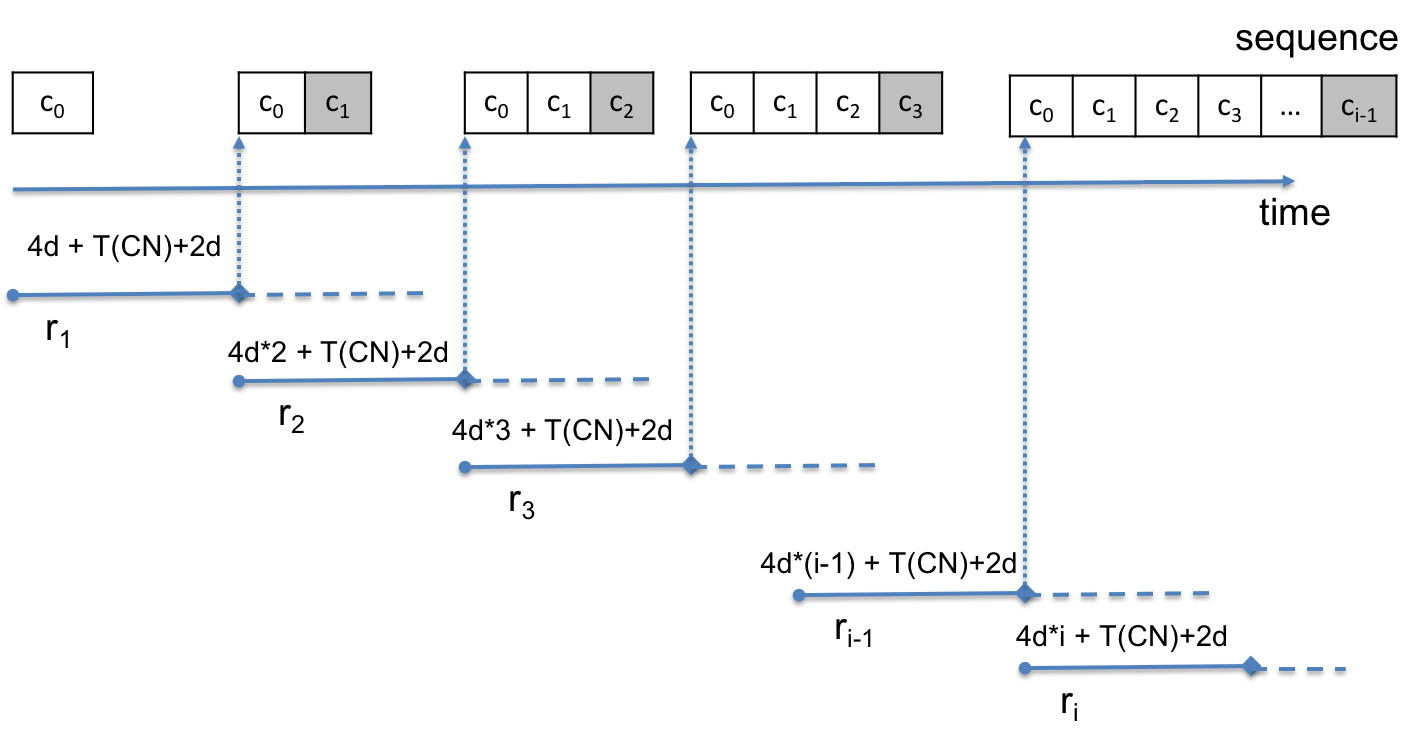
\includegraphics[width=0.60\textwidth]{reconfigExec.png}
		\caption{Successful \act{reconfig} operations.}
		\label{fig:reconfigExec}
	\end{center}
\end{figure}

More formally we can build an execution where all \act{reconfig} operations append their configuration
in the configuration sequence. Consider the partial execution $\EX$ that ends in a state $\state$. Suppose that 
every process $\pr\in\idSet$ knows the same configuration sequence, $\cvec{\pr}{\state}=\cvec{}{\state}$. Also let 
the last finalized operation in $\cvec{}{\state}$ be the last configuration of the sequence, e.g. $\mu(\cvec{}{\state}) = \nu(\cvec{}{\state})$.  
Notice that $\cvec{}{\state}$ can also be the initial configuration sequence $\cvec{\pr}{\state_0}$. 
We extend $\EX_0$ by a series of \act{reconfig} operations, such that each reconfiguration 
$\rec_i$ is invoked by a reconfigurer $r_i$ and attempts to add a configuration $c_i$. 
Let $\rec_1$ be the first reconfiguration that performs the following actions 
without being concurrent with any other \act{reconfig} operation: 
\begin{itemize}
	\item \act{read-config} starting from $\mu(\cvec{}{\state})$
	\item \act{add-config} completing both the consensus proposing $c_1$ and 
	the $\act{put-config}$ action writing the decided configuration
\end{itemize}
%\act{read-config} and \act{add-config} actions without being concurrent 
%with any other operation. 
Since  $\rec_1$ its not concurrent with any other $\act{reconfig}$ operation, then is the only process to propose
a configuration in $\mu(\cvec{}{\state})$,  and hence by the consensus algorithm properties,
$c_1$ is decided. Thus, $\cvec{}{\state}$ is appended by a tuple $\tup{c_1,P}$.

Let now reconfiguration $\rec_2$ be invoked immediately after the completion of the 
$\act{add-config}$ action from $\rec_1$. Since the local sequence at the beginning 
of $\rec_2$ is equal to $\cvec{}{\state}$, then the $\act{read-config}$ action of $\rec_2$
will also start from $\mu(\cvec{}{\state})$.  Since, $\rec_1$ already propagated $c_1$ 
to $\mu(\cvec{}{\state})$ during is $\act{put-config}$ action, then $\rec_2$ will discover 
$c_1$ during the first iteration of its $\act{read-config}$ action, and thus it will 
repeat the iteration on $c_1$. Configuration $c_1$ is the last in the sequence and 
thus the $\act{read-config}$ action of $\rec_2$ will terminate after the second 
iteration.  Following the $\act{read-config}$ action, $\rec_2$ attempts to 
add $c_2$ in the sequence. Since $\rec_1$ is the only reconfiguration that might 
be concurrent with $\rec_2$, and since $\rec_1$ already completed consensus 
in $\mu(\cvec{}{\state})$, then $\rec_2$ is the only operation to run consensus in $c_1$.
Therefore, $c_2$ is accepted and $\rec_2$ propagates $c_2$ in $c_1$ using a 
$\act{put-config}$ action. 

So in general we let configuration $\rec_i$ to be invoked after the completion of 
the $\act{add-config}$ action from $\rec_{i-1}$. As a result, the $\act{read-config}$
action of $\rec_i$ performs $i$ iterations, and the configuration $c_i$ is added 
immediately after configuration $c_{i-1}$ in the sequence. Figure \ref{fig:reconfigExec}
illustrates our execution construction for the reconfiguration operations. 

It is easy to notice that such execution results in the worst case latency for all the 
reconfiguration operations $\rec_1, \rec_2,\ldots, \rec_i$. As by Lemma \ref{lem:rcdelay}
a \act{read-config} action takes at least $4d$ time to complete, then as also 
seen in Figure \ref{fig:reconfigExec}, $k$ reconfigs may take time 
$\opdelay{k} \geq \sum_{i=1}^{k}\left[4\smdelay*i+ \left(\opdelaymin{CN}+2\smdelay\right)\right]$. Therefore, it will take time
$\opdelay{k} \geq 4\smdelay\sum_{i=1}^{k}i+ k\left(\opdelaymin{CN}+2\smdelay\right)$ and the lemma follows.
%
% We can now compute 
% the minimum latency we need to add $k$ new configurations in the configuration 
% sequence starting from the state $\state$ of execution $\EX$.
\end{proof}

The following theorem is the main result of this section, in which we define the relation between $\opdelaymin{CN}$, $d$ and $D$
%show that in any fair execution of ~\ares{}, if the  consensus operations are ``slow enough'' then  
so to guarantee that any read or write issued by a non-faulty client always terminates.

\begin{theorem}
%Consider a  read or  write operation $\pi$, invoked by a non-faulty client, in a fair and well-formed execution of ~\ares{}. Suppose at the point of invocation of $\pi$ the client has $|cseq| = p$. Then if $\opdelaymin{CN} \geq 6D(p + 2) -5d$ the operation $\pi$ completes.
 Suppose  $\opdelaymin{CN} \geq 3(6D-\smdelay)$, then  any  read or write operation $\op$ completes in any execution  $\EX$ of 
\ares{}  for any number of reconfiguration operations in $\EX$.
%$\smdelay \geq \frac{3\lgdelay}{k}-\frac{\opdelay{CN}}{2(k+2)}$
\end{theorem}

\begin{proof}
	By Lemma \ref{lem:configdelay}, 
	$k$ configurations may be installed in:
		$\opdelay{k} \geq 4\smdelay\sum_{i=1}^{k}i+ k\left(\opdelaymin{CN}+2\smdelay\right)$.	
	Also by Lemma \ref{lem:rwdelay}, we know that operation $\op$ takes at most 
$	\opdelay{\op}\leq 6\lgdelay\left(\nu(\cvec{\pr}{\state_e}) - \mu(\cvec{\pr}{\state_s})+2\right)$.
	Assuming that $k=\nu(\cvec{\pr}{\state_e}) - \mu(\cvec{\pr}{\state_s})$, the total number of 
	configurations observed during $\op$, then $\op$ may terminate before a $k+1$ configuration 
	is added in the configuration sequence if 
	  $6\lgdelay(k+2) \leq  4\smdelay\sum_{i=1}^{k}i+ k\left(\opdelaymin{CN}+2\smdelay\right)$ then we have
	  $d \geq \frac{3\lgdelay}{k}-\frac{\opdelaymin{CN}}{2(k+2)}$.
	And that completes the lemma. 
\end{proof}

\remove{

It remains now to examine if a read/write operation may ``catch up'' with any ongoing 
reconfigurations. 
For the sake of a worst case analysis we will assume that reconfiguration operations
may communicate respecting the minimum delay $\smdelay$, whereas read and write 
operations suffer the maximum delay $\lgdelay$ in each message exchange. We will
split our analysis into three directions, with respect to the number of configurations 
installed $k$, and the bound on the minimum delay $\smdelay$:
$(i)$  $k$ is finite, and $\smdelay$ may be unbounded small; $(ii)$ 
$k$ is infinite, and $\smdelay$ may be unbounded small;
$(iii)$  $k$ is infinite, and $\smdelay$ can be bounded.

\myparagraph{$k$ is finite, and $\smdelay$ may be unbounded small.}
In this case we assume a finite number of installed configurations. Also,
as the $\smdelay$ is unbounded, it follows that reconfigurations may be 
installed almost instantaneously. Let us first examine what is the maximum 
delay bound of a any read/write operation. 

\myparagraph{$k$ is infinite, and $\smdelay$ is bounded.}
We will compute the bound on $\smdelay$ with respect to the $\lgdelay$ 
and the number of configurations to be installed $k$ if we want to allow a 
read/write operation to reach ongoing reconfigurations. 

\begin{lemma} \label{lem:delaybound}
	A read/write operation $\op$ may terminate in any execution $\EX$ of 
	\ares{} given that $k$ configurations are installed during $\op$, if
	$
	\smdelay \geq \frac{3\lgdelay}{k}-\frac{\opdelaymin{CN}}{2(k+2)}
	$
\end{lemma}
%\proofremove{
\begin{proof}
	By Lemma \ref{lem:configdelay}, $k$ configurations may be installed in at least:
		$\opdelay{k} \geq 4\smdelay\sum_{i=1}^{k}i+ k\left(\opdelaymin{CN}+2\smdelay\right)$.	
	Also by Lemma \ref{lem:rwdelay}, we know that operation $\op$ takes at most 
$	\opdelay{\op}\leq 6\lgdelay\left(\nu(\cvec{\pr}{\state_e}) - \mu(\cvec{\pr}{\state_s})+2\right)$.
	Assuming that $k=\nu(\cvec{\pr}{\state_e}) - \mu(\cvec{\pr}{\state_s})$, the total number of 
	configurations observed during $\op$, then $\op$ may terminate before a $k+1$ configuration 
	is added in the configuration sequence if 
	  $6\lgdelay(k+2) \leq  4\smdelay\sum_{i=1}^{k}i+ k\left(\opdelaymin{CN}+2\smdelay\right)$ then we have
	  $d \geq \frac{3\lgdelay}{k}-\frac{\opdelaymin{CN}}{2(k+2)}$.
	And that completes the lemma. 
\end{proof}
%}
}

%\begin{theorem*}{\bf \ref{safety:ares:treas}} (Atomicity)
%	Algorithm \ares-\treas{} implements a reconfigurable atomic storage service, given that the 
%	$\act{get-data}$, $\act{get-tag}$, and $\act{put-data}$ primitives used satisfy properties
%	\textbf{C1} and \textbf{C2} of Definition \ref{def:consistency}.
%\end{theorem*}
%
%\begin{proof}
%The figure above \ref{fig:reconfig:ares:treas}
%\end{proof}


\subsection{Storage and Communication Costs for \ares{}.}\label{sec:safety:c}
Storage and Communication costs for \ares{} highly depends on the DAP that we use 
in each configuration. For our analysis we assume that each configuration utilizes the 
algorithms and the DAPs presented in Section \ref{ssec:dap:impl}.
% We now briefly present the storage and communication costs associated with the presented DAPs.
%{\treas{}  %Due to space limitations the proofs appear in \cite{}.

Recall that by our assumption, the storage cost counts the size (in bits) of the coded elements 
%that are locally stored, which are 
stored in variable $List$  at each server. We ignore the storage cost due to meta-data.
For  communication cost we measure the bits sent on the wire between the nodes.

\begin{lemma}\label {thm:storage_TREAS}
	The worst-case total storage cost of Algorithm \ref{fig:casopt} is $(\delta +1 )\frac{n}{k}$.
\end{lemma}
\begin{proof}
  The maximum number of  (tag, coded-element) pair in the $List$ is $\delta+1$, and the size of each coded element is 
  $\frac{1}{k}$ while the tag variable is a metadata and therefore, not counted. So, the total storage cost is $(\delta +1)\frac{n}{k}$.
\end{proof}

We next state  the communication cost for the write and read operations in  Aglorithm \ref{fig:casopt}. Once again, note that we ignore the communication cost arising from exchange of meta-data.

\begin{lemma} \label{treas:write_cost}
	The communication cost associated with a successful  write operation in Algorithm \ref{fig:casopt} is at most $\frac{n}{k}$. 
\end{lemma}

\begin{proof}
  During read operation, in the $\act{get-tag}$ phase the servers respond with their highest tags variables, which are metadata. However, in the $\act{put-data}$ phase, the reader sends each server the  coded elements of size  $\frac{1}{k}$ each, and hence the total cost of communication for this is $\frac{n}{k}$. Therefore, we have the worst case communication cost of a write operation is $ \frac{n}{k}$.
\end{proof}

\begin{lemma} \label{radonc:read_cost}
	The communication cost associated with a successful read operation in Algorithm \ref{fig:casopt} is at most $(\delta +2)\frac{n}{k}$. 
\end{lemma}
\begin{proof}
  During read operation, in the $\act{get-data}$ phase the servers respond with their $List$ variables and hence each such list 
  is of size at most $(\delta +1)\frac{1}{k}$, and then counting all such responses give us $(\delta +1)\frac{n}{k}$.  In the $\act{put-data}$ phase, the reader sends each server the  coded elements of size  $\frac{1}{k}$ each, and hence the total cost of communication for this is $\frac{n}{k}$. Therefore, we have the worst case communication cost of a read operation is 
  $(\delta+2) \frac{n}{k}$.
\end{proof}

From the above Lemmas we get.

\begin{theorem}\label{treas:performance}
 The \ares{} algorithm has: (i) storage cost $(\delta +1 )\frac{n}{k}$, (ii) communication 
cost for each write at most to $\frac{n}{k}$, and (iii) communication 
cost for each read at most $(\delta +2)\frac{n}{k}$.
\end{theorem}


%\section{\treas: A new two-round erasure-code based algorithm}\label{sec:treas}
%
			In this section, we present an implementation of the DAPs,  that satisfies the properties in Property~\ref{property:dap},  for a configuration $c$,  with $n$ servers 
			 using a $[n, k]$ MDS coding scheme for storage. We implement an instance of the algorithm in a 
			%Atomicity is always guaranteed. 
 configuration of  $n$ server processes. 
 We store each coded element $c_i$, corresponding to an object  at server $s_i$, where $i=1, \cdots, n$.
			% However, liveness is  guaranteed under the assumption that the number of write operations concurrent with a read  operation is at most $\delta$. The precise definition of concurrency depends on the algorithm itself, and appears later in this section. The \treas{}~algorithm has significantly reduced storage and communication cost, compared to replication, when $\delta$ is limited.
			%
%
%Expressing an atomic algorithm in terms of the DAP primitives serves multiple purposes.
%First, describing an algorithm according to template algorithm $A_1$  allows one to proof
%that the algorithm is \textit{safe} (atomic) 
%% it enables ease of reasoning about the safety of the algorithm  
%% given that atomicity holds if 
%by just showing that the appropriate DAP properties hold, and the algorithm is \textit{live} if the 
%implementation of each primitive is live. 
%Secondly, the safety and liveness proofs for more complex algorithms (like \ares{} in Section \ref{sec:ares}) % algorithm  
%become easier as one may reason on the DAP properties that are satisfied by the primitives used,
%without involving the underlying implementation of those primitives. 
%Moreover, describing a reconfiguration algorithm using DAPs, provides the flexibility 
%to vary the  implementations DAPs from configuration to configuration, as long as the DAPs satisfy certain  properties. 
%%
%%is easier where  complex operations like reconfiguration is done, where the implementation of data-access primitives can vary from one configuration to another,  while
%%hiding the details of the underlying atomic algorithm implementation. 
%%
%%
%%As we show 
%%In Section \ref{sec:algorithm}, we discuss how \ares{} may change the primitives mechanisms
%%such data access primitives allows us to design 
%%a reconfigurable atomic storage service that can utilize different atomic implementation 
%%in each established configuration without affecting the safety guarantees of the service.
%%Such approaches can adapt to the configuration design, and vary the performance of the service
%%based on the environmental conditions.
%% In other words, ABD \cite{ABD96} can be used for 
%%maximum fault tolerance and when majority quorums are used, whereas fast algorithms 
%%similar to the ones presented in \cite{CDGL04, FNP15}, could be used in configurations 
%%that satisfy the appropriate participation bounds. 
%
%
 The implementations of DAP primitives used in \ares{} are shown  
%\nnrev{by implementing the}{the} 
%DAP primitives \nnrev{as}{are implemented} 
in Alg.~\ref{fig:casopt}, and the servers' responses in Alg.~\ref{fig:casopt:server}.
%At a high level, both the read and write operations take two phases to complete (similar to the ABD algorithm).
	%, and each consists of two phases. 
	%As in algorithm $A_1$, a write operation  
%$\pi$,  \nnrev{ the writer  selects}{discovers} the maximum tag $t^*$ from
% a quorum in $\quorums{c}$ by executing $\dagettag{c}$;  creates  a new tag $t_w = tag(\pi) =  (t^*.z + 1, w)$ by 
 %incorporating the writer's own ID; and 
%it performs a $c.\act{put-data}(\tup{t_w, v})$ to propagate that pair to a quorum in $c$.
%A read operation performs $\dagetdata{c}$ to retrieve a tag-value pair, $\tup{\tg{},v}$ form configuration $c$, and then 
%it performs a $c.\act{put-data}(\tup{\tg{},v})$ to propagate that pair to the servers $\servers{c}$. 

%A write operation is similar to the read but before 
%performing the $\act{put-data}$ action it generates a new tag which associates with the value to be written. 
%

%\begin{algorithm}[!ht]
%		\begin{algorithmic}[2]
%			\begin{multicols}{2}
%				{\footnotesize
%					%\Part{Generic Algorithm $A_1$}
%					\Operation{read}{} 
%					%\State $wCounter\gets wCounter+1$
%					\State $\tup{t, v} \gets \dagetdata{c}$
%					\State $\daputdata{c}{ \tup{t,v}}$
%					\State return $ \tup{t,v}$
%					\EndOperation
%					\Statex
%					\Operation{write}{$v$} 
%					%\State $wCounter\gets wCounter+1$
%					\State $t \gets \dagettag{c}$
%					\State $t_w \gets \tup{t.z + 1,  w}$
%					\State $\daputdata{c}{\tup{t_w,v}}$
%					\EndOperation
%					%\EndPart
%				}
%			\end{multicols}
%			\end{algorithmic}
%		\caption{Read and write operations of algorithm template $A_1$}
%		\label{algo:atomicity:generic1}
%		\vspace{-1em}
%	\end{algorithm}
%		\newcommand{\algrule}[1][.2pt]{\par\vskip.5\baselineskip\hrule height #1\par\vskip.5\baselineskip}	
			\begin{algorithm*}[!ht]
				\begin{algorithmic}[2]
					{\small
					\begin{multicols}{2}
							\State{ at each process $\pr_i\in\idSet$}
							%\remove{
%										{\scriptsize
%				%\Part{Generic Algorithm $A_1$}
%				\Operation{read}{} 
%				%\State $wCounter\gets wCounter+1$
%				\State $\tup{t, v} \gets \dagetdata{c}$
%				\State $\daputdata{c}{ \tup{t,v}}$
%				\State return $ \tup{t,v}$
%				\EndOperation
%				\Statex
%				\Operation{write}{$v$} 
%				%\State $wCounter\gets wCounter+1$
%				\State $t \gets \dagettag{c}$
%				\State $t_w \gets inc(t)$
%				\State $\daputdata{c}{\tup{t_w,v}}$
%				\EndOperation
%				%\EndPart
%			}%}
	
							\Statex
							\Procedure{c.get-tag}{}
							%	\State {\bf send} $(\text{\act{query}},\rdr)$ to every server $s\in \bigcup_{cseq[i]}members(\qs_{cseq[i].conf})$
							\State {\bf send} $(\text{{\sc query-tag}})$ to each  $s\in \servers{c}$
							\State {\bf until}   $\pr_i$ receives $\tup{t_s,e_s}$ from $\left\lceil \frac{n + k}{2}\right\rceil$ servers in $\servers{c}$
							\State $t_{max} \gets \max(\{t_s : \text{ received } \tup{t_s,v_s} \text{ from } s \})$
							\State {\bf return} $t_{max}$
							\EndProcedure
							
							\Statex
							
							\Procedure{c.get-data}{}
							%	\State {\bf send} $(\text{{\sc query}},\rdr)$ to every server $s\in \bigcup_{cseq[i]}members(\qs_{cseq[i].conf})$
								\State {\bf send} $(\text{{\sc query-list}})$ to each  $s\in \servers{c}$
								\State {\bf until}    $\pr_i$ receives $List_s$ from each server $s\in\srvSet_g$ s.t. $|\srvSet_g|=\left\lceil \frac{n + k}{2}\right\rceil$ and  $\srvSet_g\subset \servers{c}$ 
								\State  $Tags_{*}^{\geq k} = $ set of tags that appears in  $k$ lists	\label{line:getdata:max:begin}
								\State  $Tags_{dec}^{\geq k} =$ set of tags that appears in $k$ lists with values
								\State  $t_{max}^{*} \leftarrow \max Tags_{*}^{\geq k} $
                                \State  $t_{max}^{dec} \leftarrow \max Tags_{dec}^{\geq k} $ \label{line:getdata:max:end}
								\If{ $t_{max}^{dec} =  t_{max}^{*}$} 
								    \State  $v \leftarrow $ decode value for $t_{max}^{dec}$
								\EndIf
								%\State $List_M \triangleq \bigcup_{s \in \srvSet_g}  List_s$
								%$\State  $\forall t$, $List_M(t) \triangleq \{ (t, v): (t,v) \in List_M \}$  
								%\State $\forall t$, $T(t') \triangleq \{t: (t,v) \in List_M(t) \wedge t \geq t' \}$
								%\State $t_r \gets \max \{t : (t, *) \in List_M ~\wedge |List_M(t)| \geq k~\wedge |T(t)| \leq \delta \}$
								%\State $v_s\gets \text{decode from }  List_M(t_{r}))$
								\State {\bf return} $\tup{t^{dec}_{max},v}$
							\EndProcedure
							
							\Statex				
							
							\Procedure{c.put-data}{$\tup{\tg{},v})$}
								\State $\Coded = [(\tg{}, e_1), \ldots, (\tg{}, e_n)]$, $e_i = \Phi_i(v)$
								\State {\bf send} $(\text{{\sc write}}, \tup{\tg{},e_i})$ to each $s_i \in \servers{c}$
								\State {\bf until} $\pr_i$ receives {\sc ack} from $\left\lceil \frac{n + k}{2}\right\rceil$ servers in $\servers{c}$
							\EndProcedure
							%\EndPart
							
							
							
%							\Part{write($v$)}\EndPart
%							\Part{\underline{\GetTag}} {
%								\State  Send  $(\QueryTag)$ to all servers $\mathcal{S}$.
%								\State  Await responses from majority
%								\State  Select the max tag  $t^*$
%							}\EndPart
%							\Statex
%							\Part{\underline{\PutData}} {
%								\State $t_w = (t^{*}.z + 1, w)$.  
%								\State $\Coded = [(t_w, c_1), \ldots, (t_w, c_n)]$, $c_i = \Phi_i(v)$
%								\State Send  $(\CodedElementTag, \Coded)$ to all servers $\mathcal{S}$.
%								\State Terminate after $\left\lceil \frac{n + k}{2}\right\rceil$ acks
%							}	\EndPart
							
%							\Statex
%							\Part{read}\EndPart
%							\Part{\underline{\GetData}} {
%								\State  Send $(\QueryList)$ to all servers $\mathcal{S}$.
%								\State  Wait for $\left\lceil \frac{n+k}{2}\right\rceil$ $Lists$ 
%								\State  Select the max tag, $t_r$, the corresponding value, $v_r$, is decodable using the $Lists$; additionally   $t_r$ is among the highest distinct $\delta$ tags received in any $Lists$.
%							}\EndPart	
%							\Statex
%							\Part{\underline{\PutData}} {
%								\State $\Coded = [(t_r, c_1), \ldots, (t_r, c_n)]$, $c_i = \Phi_i(v_r)$
%								\State Send $(\CodedElementTag, \Coded)$ to all servers $\mathcal{S}$.
%								\State Wait for $\left\lceil \frac{n + k}{2}\right\rceil$ acks
%								\State Return $v_r$
%							}	\EndPart
%							
%							
					\end{multicols}
				}
				\end{algorithmic}	
				\caption{DAP implementation 
					%for  template $A_1$ to implement 
					for  \ares{}. }
				\label{fig:casopt}
				\vspace{-1em}
			\end{algorithm*}
		

	\begin{algorithm*}[!ht]
	\begin{algorithmic}[2]
		{\small
		\begin{multicols}{2}
				\State{at each server $s_i \in \mathcal{S}$ in configuration $c_k$}
				\Statex
				\State{\bf State Variables:}%{ 										
					%\Statex $(t_{loc}, v_{loc}) \in \mathcal{T} \times {\mathcal V}$, initially   $(t_0, v_0)$
					%\Statex $status \in \{active, repair\}$, initially $active$
					\Statex $List \subseteq  \mathcal{T} \times \mathcal{C}_s$, initially   $\{(t_0, \Phi_i(v_0))\}$
				%}\EndPart
			
			\Statex
			\Receive{{\sc query-tag}}{$s_i,c_k$}
				\State $\tg{max} = \max_{(t,c) \in List}t$
				\State Send $\tg{max}$ to $q$
			\EndReceive
			\Statex
	
			
			\Receive{{\sc query-list}}{$s_i,c_k$}
				\State Send $List$ to $q$
			\EndReceive
\State
			\Receive{{\sc put-data}, $\tup{\tg{},e_i}$}{$s_i,c_k$}
				\State $List \gets List \cup \{ \tup{\tg{}, e_i}  \}$ 
				\If{$|List| > \delta+1$}
					\State $\tg{min}\gets\min\{t: \tup{t,*}\in List\}$
				%	\Statex
                                              \Statex  ~~~~~~~~/* remove the coded value and retain the tag */
					%\State $List \gets List \backslash~\{\tup{\tg{},e}: \tg{}=\tg{min} ~\wedge~\tup{\tg{},e}\in List\} \cup \{  (  \tg{min}, \bot)  \}$\label{line:server:removemin}
					\State $List \gets List \backslash~\{\tup{\tg{},e}: \tg{}=\tg{min} ~\wedge \tup{\tg{},e}\in List\}$
					\State $List \gets List  \cup \{  (  \tg{min}, \bot)  \}$\label{line:server:removemin}
				\EndIf
				\State  Send {\sc ack} to $q$
			\EndReceive
			
%				\Statex
%				\Part {\underline{\GetTagResp,recv $\QueryTag$ from writer $w$}} {
%					%\If{ $status = active$ }
%					\State $t^* = \max_{(t,c) \in List}t$
%					\State Send $t^*$ to $w$
%					\Statex %\EndIf
%				}\EndPart
%				%										\Statex
%				\Part {\underline{\GetDataResp, recv $\QueryList$ from reader $r$}} {
%					%\If{ $status = active$ }
%					\State Send  $List$ to $r$
%					%\EndIf
%				}\EndPart
%				%	
%				\Statex
%				\Part{ \underline{\PutDataResp, recv $\CodedElementTag, (t, c_i)$ from $p$ }}{
%					%\If{$status = active$}
%					\State $List \leftarrow List \cup \{ (t, c_i)  \}$ 
%					\If{ $|List| > \delta + 1$ } 
%					\State  Retain the (tag, coded-element) pairs for the $\delta +1 $ highest tags in $List$, and delete the rest.
%					\EndIf 
%					\State  Send ack to $p$.
%					%\EndIf
%					
%				}\EndPart
				\end{multicols}
			}
	\end{algorithmic}	
	\caption{The response protocols at  any server $s_i \in {\mathcal S}$ in  
					\ares{} for client requests.}\label{fig:casopt:server}
					\vspace{-1em}
\end{algorithm*}		
 Each server $s_i$ stores one  state variable,  $List$,  which is a set of up to $(\delta + 1)$  (tag, coded-element) pairs. Initially the set at $s_i$ contains a single element, $List = \{ (t_0,  \Phi_i(v_0)\}$.   Below we describe the implementation of the DAPs.
%
%				At a high-level, the algorithm (see Fig.~\ref{fig:casopt}) is a natural generalization of the $ABD$ algorithm accounting for the fact that we use MDS codes.
	
$\dagettag{c}$: A  client,  during the execution of a  $\dagettag{c}$ primitive, queries all the servers in $\servers{c}$ for the highest tags in their  $Lists$, and awaits responses from $\left\lceil \frac{n+k}{2} \right\rceil$ servers.
% with $k \geq \frac{2n}{3}$. 
A server upon receiving the {\sc get-tag} request, 
responds to the client with the highest tag, as $\tg{max} \equiv \max_{(t,c) \in List}t$. 
Once the client receives the tags from $\left\lceil \frac{n+k}{2} \right\rceil$ servers,  it selects  the highest  tag $t$ and returns it . 
							
 $c.\act{put-data}(\tup{t_w, v})$: During the  execution of the primitive  $c.\act{put-data}(\tup{t_w, v})$,  a client 
 % computes the coded elements for each of the $n$ servers, and 
 sends the  pair  $(t_w, \Phi_i(v))$ to each server $s_i\in\servers{c}$.  
 When a server $s_i$ receives a message $(\text{\sc put-data}, t_w, c_i)$ , it adds the pair in its local $List$, 
 trims the pairs with the smallest tags exceeding the length $(\delta+1)$ of the $List$ , and replies 
 with an ack to the client.
 %
 %Every time a $(\text{\sc put-data}, t_w, c_i)$  message arrives at a server $s_i$, 
 %from a writer, 
 %the pair gets added to the $List$. As the size of the $List$ at each $s_i$ is bounded by $(\delta+1)$, then following an insertion in the $List$, $s_i$ trims the coded-elements associated with the smallest tags. 
 In particular, $s_i$ replaces the coded-elements of the older tags with $\bot$, and maintains only the coded-elements associated with the 
 	$(\delta+1)$ highest tags in the $List$ (see Line Alg.~\ref{fig:casopt:server}:\ref{line:server:removemin}).
 %which is then garbage collected to keep tag and coded-element pairs of the highest  $(\delta+1)$ tags, and by replacing the coded-elements of the older tags with $\bot$,  a symbol that signifies garbage-collected coded-elements. 
  The client completes the primitive operation after getting acks from $\left\lceil \frac{n+k}{2} \right\rceil$ servers.
			
	$\dagetdata{c}$:	A  client, during the execution of a  $\dagetdata{c}$ primitive, queries all the servers in $\servers{c}$ for their  local variable $List$, and awaits responses from $\left\lceil \frac{n+k}{2} \right\rceil$ servers. Once the client receives $Lists$ from $\left\lceil \frac{n+k}{2} \right\rceil$ servers,  it selects the highest  tag $t$, such that: $(i)$ its corresponding value $v$ is decodable from the coded elements in the lists; and $(ii)$ $t$ is the highest tag seen from the responses of at least $k$ $Lists$ 
			(see lines Alg.~\ref{fig:casopt}:\ref{line:getdata:max:begin}-\ref{line:getdata:max:end}) and returns the pair $(t, v)$. 
Note that in the case where anyone of the above conditions is not satisfied the corresponding read operation does not complete.
% \newpage
%\begin{theorem} \label{thm:storage_TREAS}
%	The worst-case total storage cost of \treas{} algorithm is  $(\delta +1 )\frac{n}{k}$.
%\end{theorem}
%\proofremove{
%	\begin{proof}
%		The maximum number of  (tag, coded-element) pair in the $List$ is $\delta+1$, and the size of each coded element is 
%		$\frac{1}{k}$ while the tag variable is a metadata and therefore, not counted. So, the total storage cost is $(\delta +1)\frac{n}{k}$.
%	\end{proof}
%}
%
%We next state  the communication cost for the write and read operations in  \treas{}. Once again, note that we ignore the communication cost arising from exchange of meta-data.
%
%\begin{theorem} \label{treas:write_cost}
%	The communication cost associated with a successful  write operation in \treas{} is at most $\frac{n}{k}$. 
%\end{theorem}
%\proofremove{
%	\begin{proof}
%		During read operation, in the $\act{get-tag}$ phase the servers responds with their highest tags variables, which are metadata. However, in the $\act{put-data}$ phase, the reader sends each server the  coded elements of size  $\frac{1}{k}$ each, and hence the total cost of communication for this is $\frac{n}{k}$. Therefore, we have the worst case communication cost of a write operation is $ \frac{n}{k}$.
%	\end{proof}
%}
%\begin{theorem} \label{radonc:read_cost}
%	The communication cost associated with a successful read operation in \treas{} is at most $(\delta +2)\frac{n}{k}$. 
%\end{theorem}
%\proofremove{
%	\begin{proof}
%		During read operation, in the $\act{get-data}$ phase the servers responds with their $List$ variables and hence each such list 
%		is of size at most $(\delta +1)\frac{1}{k}$, and then counting all such responses give us $(\delta +1)\frac{n}{k}$.  In the $\act{put-data}$ phase, the reader sends each server the  coded elements of size  $\frac{1}{k}$ each, and hence the total cost of communication for this is $\frac{n}{k}$. Therefore, we have the worst case communication cost of a read operation is 
%		$(\delta+2) \frac{n}{k}$.
%	\end{proof}
%}
%

\section{Correctness,  performance and latency  of \ares{}}\label{sec:ares_safety}
In this section, we prove the atomicity property of \ares{}. We also provide an analysis of its storage and communication costs, and the 
latency of read and write operations. The atomicity property of \ares{} hinges on the Property~\ref{property:dap} 
of the DAP implementation in each individual configuration used in~\ares{}. Therefore, we start by proving, in subsection~\ref{sec:safety:a},  that 
Property~\ref{property:dap} holds for the DAP implementation in Section~\ref{ssec:dap:impl}. 
Based on this, in subsection ~\ref{sec:safety:b}, we prove the atomicty of \ares{}. Next, in sub-section~\ref{sec:safety:c}, we derive the storage
and communication costs of read and write operations, and in sub-section ~\ref{sec:safety:d}, we derive the latency
of reads and writes in terms of the minimum and maximum delays of any point-to-point messages of the 
underlying network.
Due to lack of space proofs are omitted and can be found in the 
% of the following Theorem is produced in the 
extended version of the paper~\cite{ARES:Arxiv:2018}.	

\subsection{Safety (Property~\ref{property:dap})  proof of the DAP{s}}\label{sec:safety:a}
%\vspace{-1.em}
\myparagraph{Correctness.} 
In this section we are concerned with only one configuration $c$, consisting of a set of servers 
%$\mathcal{S}$
$\servers{c}$.
%, and a set of reader and writer clients $\mathcal{R}$ and $\mathcal{W}$, respectively. In other words, 
%in such static system the sets $\mathcal{S}$, $\mathcal{R}$ and $\mathcal{W}$ are fixed, and 
We assume that at most $f \leq \frac{n-k}{2}$ servers from $\servers{c}$ may crash.  
Lemma~\ref{casflex:data-access:consistent} states that the DAP implementation 
 satisfies the  consistency properties Property~\ref{property:dap}  which will be used to 
%of \treas{}, \nn{and in turn by Theorem \ref{atomicity:A1}} these 
imply the atomicity of the \ares{} algorithm. 
%which implies the atomicity city properties and consequently the
%atomicity property 
%(Theorem~\ref{thm:atomicity_radonc}).			
%\myparagraph{Liveness and Safety Conditions.}\blue{
%The \treas{} algorithm we present satisfy \myemph{wait-free termination} (Liveness) and \myemph{atomicity} (Safety).
%}
	%Due to lack of space the proof of the following Theorem is produced in the Appendix.	
\label{sec:primitives}

%
% 
% This abstraction enables us to prove the safety and liveness properties of such algorithms based on the properties of these primitives. 
% This abstraction servers us a two-fold 
% purpose: $(i)$ by expressing several atomicity emulation algorithm in terms of the primitives allows us to prove safety and liveness based on their properties $(iii)$ shows how such algorithms can be adopted to our ARES algorithm and prove their safety and liveness without; and $(iii)$ exposes the intuition that the underlying atomicity algorithm can  be different from configuration to configuration.
% For version control of the  object values  we use tags.  
% 
 
 
 %Let $<_\tau$ and $\leq_\tau$ be the appropriate comparison relationships used by any algorithm 
 %that utilizes logical timestamps. Then 
 %atomicity properties can be expressed in terms of the tags written and returned by write and read 
 %operations respectively. 
 %For a write operation $\wrt$ we denote by $\tg{\wrt}$ the tag that is 
 %used by $\wrt$ and for a read $\rd$ we denote by $\tg{\rd}$ the tag that is returned by $\rd$
 %\footnote{Note that the values written or returned by write of read operations can be mapped easily  
 %to the tags they write or return.}.	The partial ordering among the  operations  can then be induced from the partial ordering among the tags. 
 %using  tags in the following way: (i) for any two write 
 %operations $\wrt_1$, $\wrt_2$, if  $\wrt_1\prec\wrt_2$, then $\tg{\wrt_1}<_\tau\tg{\wrt_2}$,
 %(ii) For any operation $\op_1$,  and any read operation $\rd_2$, if $\op_1\prec\rd_2$, then
 %$\tg{\op_1}\leq_\tau\tg{\rd_2}$.

\proofremove{
 \begin{proof}
 We  prove the atomicity by proving properties $P1$, $P2$ and $P3$ appearing in Lemma \ref{XXX} for any execution of the algorithm.
					
	\emph{Property $P1$}: Consider two operations $\phi$ and $\pi$ such that $\phi$ completes before $\pi$ is invoked. 
	We need to show that it cannot be  the case that $\pi \prec \phi$. We break our analysis into the following four cases:

	Case $(a)$: {\em Both $\phi$ and $\pi$ are writes}. The $\daputdata{c}{*}$ of $\phi$ completes before 
	$\pi$ is invoked. 
	%which implies that by well-formedness 
	By property $C1$ the tag $\tg{\pi}$ returned by the $\dagetdata{c}$ at $\pi$ is 
	at least as large as $\tg{\phi}$. Now, 
	%since $\tg{\pi}$ is larger than $t_{\phi}$, by the steps of 
	since $\tg{\pi}$ is incremented by the write operation then $\pi$ puts a tag $\tg{\pi}'$ such that
	$\tg{\phi} < \tg{\pi}'$ and hence we cannot have $\pi \prec \phi$.
	
	Case $(b)$: {\em $\phi$ is a write and  $\pi$ is a read}. In execution $\EX$ since 
$\daputdata{c} {\tup{t_{\phi}, *}}$ of $\phi$ completes 
	before the $\dagetdata{c}$ of $\pi$ is invoked, by 
	%the well-formedness 
	property $C1$ the tag $\tg{\pi}$ obtained from the above
	$\dagetdata{c}$ is at least as large as $\tg{\phi}$. Now $\tg{\phi} \leq \tg{\pi}$ implies that we cannot have $\pi \prec \phi$.
	
	Case $(c)$: {\em $\phi$ is a read and  $\pi$ is a write}.  Let the id of the writer that invokes $\pi$ we $w_{\pi}$.  
	The 
$\daputdata{c}{\tup{\tg{\phi}, *}}$  call of $\phi$ completes
	before  $\dagettag{c}$ of $\pi$ is initiated. Therefore, by 
	%the well-formedness 
	property $C1$ %of data-primitives the above 
	$\act{get-tag}(c)$ returns $\tg{}$ such that, $\tg{\phi} \leq \tg{}$. Since $\tg{\pi}$ is equal to $(\tg{}.z + 1, w_{\pi})$ 
	by design of the algorithm, hence $\tg{\pi} > \tg{\phi}$ and we cannot have $\pi \prec \phi$.
	
	Case $(d)$: {\em Both $\phi$ and $\pi$ are reads}. In execution $\EX$  
the $\daputdata{c}{\tup{t_{\phi}, *}}$ is executed as a part of $\phi$ and 
	completes before $\dagetdata{c}$ is called in $\pi$. By 
	%the well-formedness
	 property $C1$ of the data-primitives, 
	we have $\tg{\phi} \leq \tg{\pi}$ and hence we cannot have $\pi \prec \phi$.
	
	\emph{Property $P2$}: Note that because $\tsSet$ is well-ordered we can show that this property by first showing that
	every write has a unique tag. This means any two pair of writes can be ordered. Now, a read can be ordered . Note that 
	a read can be ordered w.r.t. to any write operation trivially if the respective tags are different, and by definition, if the 
	tags are equal the write is ordered before the read.
	
	Now observe that two tags generated from two write operations from different writers are necessarily distinct because of the 
	id component of the tag. Now if the operations, say $\phi$ and $\pi$ are writes  from the same writer then by 
	well-formedness property the second operation is invoked after the first completes, say without loss of generality $\phi$ completes before 
	$\pi$ is invoked.   In that case the integer part of the tag of $\pi$ is higher 
	%because the well-formedness 
	by property  $C1$, and since the $\dagettag{c}$  is followed by $\daputdata{c}{*}$. Hence $\pi$ is ordered after $\phi$. 
	
	\emph{Property $P3$}:  This is clear because the tag of a reader is defined by the tag of the value it returns by property (b).
	Therefore, the reader's immediate previous value it returns. On the other hand if  does 
	note return any write operation's value it must return $v_0$.
 \end{proof}
}



						
 \begin{theorem}[Safety]\label{casflex:data-access:consistent}
Let $\Pi$ a set of complete DAP operations of Algorithm \ref{fig:casopt} in a configuration $c\in\confSet$,
$\act{c.get-tag}$, $\act{c.get-data}$ and $\act{c.put-data}$,
of an execution $\EX$. Then, every pair of operations $\phi,\op\in\Pi$ satisfy Property \ref{property:dap}.
% The data-access primitives, i.e., $\act{get-tag}$, $\act{get-data}$ and $\act{put-data}$ primitives implemented in any configuration  $c$
% in this section satisfy Property~\ref{property:dap}.
\end{theorem}


\proofremove{
\begin{proof}
As mentioned above we are concerned with only configuration $c$, and therefore, in our proofs we will be concerned with only one
configuration. Let $\alpha$ be some execution of \treas{}, then we consider two cases for $\pi$ for proving property $C1$:  $\pi$ is a  $\act{get-tag}$ operation, or $\pi$ is a $\act{get-data}$ primitive. 

 %\item[ C1 ]  If $\phi$ is a  $\daputdata{c}{\tup{\tg{\phi}, v_\phi}}$, for $c \in \confSet$, $\tg{1} \in\tsSet$ and $v_1 \in \valSet$,
 %and $\pi$ is a $\dagettag{c}$ (or a $\dagetdata{c}$) 

 %that returns $\tg{\pi} \in \tsSet$ (or $\tup{\tg{\pi}, v_{\pi}} \in \tsSet \times \valSet$) and $\phi$ completes before $\pi$ in $\EX$, then $\tg{\pi} \geq \tg{\phi}$.
Case $(a)$: $\phi$ is   $\daputdata{c}{\tup{\tg{\phi}, v_\phi}}$ and  $\pi$ is a $\dagettag{c}$ returns $\tg{\pi} \in \tsSet$. Let $c_{\phi}$ and $c_{\pi}$ denote the clients that invokes $\phi$ and $\pi$ in $\alpha$. Let $S_{\phi} \subset \mathcal{S}$ denote the set of $\left\lceil \frac{n+k}{2} \right \rceil$ servers that responds to $c_{\phi}$, during $\phi$. Denote by $S_{\pi}$ the set of $\left\lceil \frac{n+k}{2} \right \rceil$ servers that responds to $c_{\pi}$, during $\pi$.  Let $T_1$ be a point in execution $\alpha$ 
after the completion of $\phi$ and before the invocation of $\pi$. Because $\pi$ is invoked after $T_1$, therefore, at $T_1$ each of the servers in $S_{\phi}$ contains $t_{\phi}$ in its $List$ variable. Note that, once a tag is added to $List$, it is never removed. Therefore, during $\pi$, any server in $S_{\phi}\cap S_{\pi}$ responds with $List$ containing $t_{\phi}$ to $c_{\pi}$. Note that since  $|S_{\sigma^*}| = |S_{\pi}| =\left\lceil \frac{n+k}{2} \right \rceil $ implies
				 $| S_{\sigma^*} \cap S_{\pi} | \geq k$, and hence $t^{dec}_{max}$ at $c_{\pi}$, during $\pi$ is at least as large as $t_{\phi}$, i.e., $t_{\pi} \geq t_{\phi}$. Therefore, it suffices to to prove our claim with respect to the tags and the decodability of  its corresponding value.


Case $(b)$: $\phi$ is   $\daputdata{c}{\tup{\tg{\phi}, v_\phi}}$ and  $\pi$ is a $\dagetdata{c}$ returns $\tup{\tg{\pi}, v_{\pi}} \in \tsSet \times \valSet$. 
As above, let $c_{\phi}$ and $c_{\pi}$ be the clients that invokes $\phi$ and 
$\pi$. Let $S_{\phi}$ and $S_{\pi}$ be the set of servers that responds to $c_{\phi}$ and $c_{\pi}$, respectively. Arguing as above, 
 $| S_{\sigma^*} \cap S_{\pi} | \geq k$ and every server in  $S_{\phi} \cap S_{\pi} $ sends $t_{\phi}$ in response to $c_{\phi}$, during 
 $\pi$, in their $List$'s and hence $t_{\phi} \in Tags_{*}^{\geq k}$. Now, because $\pi$ completes in $\alpha$, hence we have 
 $t^*_{max} = t^{dec}_{max}$. Note that $\max Tags_{*}^{\geq k} \geq \max Tags_{dec}^{\geq k}$ so 
  $t_{\pi} \geq \max Tags_{dec}^{\geq k} = \max Tags_{*}^{\geq k} \geq t_{\phi}$. Note that each tag is always associated with 
  its corresponding value $v_{\pi}$, or the corresponding coded elements $\Phi_s(v_{\pi})$ for $s \in \mathcal{S}$.

Next, we prove the $C2$ property of DAP for the \treas{} algorithm. Note that the initial values of the $List$ variable in each servers $s$ in $\mathcal{S}$ is 
$\{ (t_0, \Phi_s(v_{\pi}) )\}$. Moreover, from an inspection of the steps of the algorithm, new tags in the $List$ variable of any servers of any servers is introduced via $\act{put-data}$ operation. Since $t_{\pi}$ is returned by a $\act{get-tag}$ or 
$\act{get-data}$ operation then it must be that either $t_{\pi}=t_0$ or $t_{\pi} > t_0$. In the case where $t_{\pi} = t_0$ then we have nothing to prove. If $t_{\pi} > t_0$ then there must be a $\act{put-data}(t_{\pi}, v_{\pi})$ operation $\phi$. To show that for every $\pi$ it cannot be that $\phi$ completes before $\pi$, we adopt by a contradiction. Suppose for every $\pi$, $\phi$ completes before $\pi$ begins, then clearly $t_{\pi}$ cannot be returned $\phi$, a contradiction.
\end{proof}
}			
	\remove{
				\begin{theorem}[Atomicity]  \label{thm:atomicity_radonc}
					Any well-formed and fair execution of \treas{},  is atomic.
				\end{theorem}
		}
	\myparagraph{Liveness.} \label{sec:treas_liveness}
    To reason about the liveness of the proposed DAPs, we define a concurrency parameter $\delta$ which  captures all the  $\act{put-data}$ operations that overlap with the $\act{get-data}$, until the time the client has all data needed to attempt decoding a value. However, we ignore those $\act{put-data}$ operations that might have started in the past, and never completed yet, if their tags are less than that of any $\act{put-data}$ that completed before the  $\act{get-data}$  started. This allows us to ignore $\act{put-data}$ operations due to failed clients, while counting concurrency, as long as the failed $\act{put-data}$ operations are followed by a successful $\act{put-data}$ that completed before the $\act{get-data}$ started. 				
\kmk{In order to define the amount of concurrency  in  our specific implementation of the DAPs presented in this section the}  following definition captures the $\act{put-data}$ operations that overlap with the $\act{get-data}$, until  the client has all data required to  decode the value.
				
\begin{definition}[Valid $\act{get-data}$ operations]
A $\act{get-data}$  operation $\pi$ from a process $p$ is \myemph{valid}  if 
%the associated client 
$p$ does not crash until the reception of $\left\lceil \frac{n+k}{2} \right\rceil$ responses during the{\GetData} phase. 
\end{definition}
					
				
				\begin{definition}[$\act{put-data}$ concurrent with a valid $\act{get-data}$] \label{defn:concurrent}
					Consider a valid $\act{get-data}$ operation $\pi$ from a process $p$. 
					Let $T_1$ denote the point of initiation of $\pi$. For $\pi$, let $T_2$ denote the earliest point of time during the execution when $p$ 
					%the associated client 
					receives all the $\left\lceil \frac{n+k}{2} \right\rceil$ responses.
					% For a valid repair,  let $T_2$ denote the point of time during the execution when the repair completes, and takes the associated server back to the active state. 
					Consider the set $\Sigma = \{ \phi: \phi$ is any $\act{put-data}$ operation that completes before $\pi \text{ is initiated} \}$, and let $\phi^* = \arg\max_{\phi \in \Sigma}tag(\phi)$. Next, consider the set $\Lambda = \{\lambda:  \lambda$  is any $\act{put-data}$ operation that starts before $T_2 \text{ such that } tag(\lambda) > tag(\phi^*)\}$. We define the number of $\act{put-data}$ concurrent with the valid $\act{get-data}$  $\pi$ to be the cardinality of the set $\Lambda$.
				\end{definition}
							
Termination (and hence liveness)  of the DAPs is guaranteed in an execution $\EX$, provided that a process 
	no more than $f$ servers in $\servers{c}$ crash, and no more that $\delta$ $\act{put-data}$ may be concurrent at any point in $\EX$. 
	%in  property of an algorithm,  we mean that 
	If the failure model is satisfied, then any operation invoked by a non-faulty client will collect the necessary replies
	% process terminates  
	independently of the progress of any other client process in the system. Preserving $\delta$ on the other hand,
	ensures that any operation will be able to decode a written value. These are captured in the following theorem:

				\begin{theorem}[Liveness]  \label{thm:liveness_radonc}
					Let $\EX$ be well-formed and fair execution of DAPs, with an $[n, k]$ MDS code, 
					where $n$ is the number of servers out of which no more than $\frac{n-k}{2}$ may crash, 
					%and $k  > n/3$,
					 and $\delta$ be the maximum number of $\act{put-data}$ operations concurrent with any 
					 valid $\act{get-data}$ operation. 
					 Then any $\act{get-data}$ and $\act{put-data}$ operation $\op$ 
					 invoked by a process $\pr$  terminates in $\EX$ if $\pr$
					 does not crash between the invocation and response steps of $\op$.\vspace{-.5em}
				\end{theorem}
		\proofremove{		
				\begin{proof}
				Note that in the read and write operation the  $\act{get-tag}$ and $\act{put-data}$ operations initiated by any non-faulty client  always complete.
				Therefore, the liveness property with respect to any write operation is clear because it uses only  $\act{get-tag}$ and $\act{put-data}$ operations of the DAP. So, we focus on proving the liveness property of any read operation $\pi$, 
				specifically,   the  $\act{get-data}$ operation completes. Let $\alpha $ be and execution of \treas{} and let 
				$c_{\sigma^*}$ and $c_{\pi}$ be the clients that invokes the write operation $\sigma^*$ and 
				read operation $c_{\pi}$, respectively.
				
				Let $S_{\sigma^{*}}$ be the set of 
				$\left\lceil \frac{n+k}{2} \right \rceil$ servers that responds to 
				$c_{\sigma^*}$, in the $\act{put-data}$ operations, in $\sigma^*$.
				 Let $S_{\sigma^{\pi}}$ be the set of $\left\lceil \frac{n+k}{2} \right \rceil$ servers that responds to  $c_{\pi}$ during the  $\act{get-data}$ step of $\pi$. Note that in $\alpha$ at the point execution $T_1$, just before the execution of  $\pi$, none of the the write operations in 
				 $\Lambda$ is complete. Observe that,  by algorithm design, the coded-elements corresponding to  $t_{\sigma^*}$ are garbage-collected from the $List$ variable of a server only if more than $\delta$ higher tags are introduced by subsequent writes into the server.  Since the number of concurrent writes  $|\Lambda|$, s.t.  $\delta > | \Lambda |$ the corresponding value of tag $t_{\sigma^*}$ is not garbage collected in $\alpha$, at least until execution point $T_2$  in  any of the servers in $S_{\sigma^*}$.
				 
				 Therefore, during the execution fragment between the execution points $T_1$ and $T_2$ of the execution $\alpha$, the tag and coded-element pair is present in the $List$ variable of every in $S_{\sigma^*}$ that is active. As a result, the tag and coded-element pairs, $(t_{\sigma^*}, \Phi_s(v_{\sigma^*}))$ exists in the $List$ received from any
				  $s \in S_{\sigma^*} \cap S_{\pi}$ during operation $\pi$. Note that since $|S_{\sigma^*}| = |S_{\pi}| =\left\lceil \frac{n+k}{2} \right \rceil $ hence
				 $| S_{\sigma^*} \cap S_{\pi} | \geq k$ and hence 
				 $t_{\sigma^*} \in Tags_{dec}^{\geq k} $, the set of decodable tag, i.e., the value $v_{\sigma^*}$ can be decoded
				  by $c_{\pi}$ in $\pi$, which demonstrates that $Tags_{dec}^{\geq k}  \neq \emptyset$. Next we want to 
				  argue that 
				  $t_{max}^* = t_{max}^{dec}$ via a contradiction: we assume 
				  $ \max Tags_{*}^{\geq k}  >  \max Tags_{dec}^{\geq k}  $. Now, consider any tag $t$, which  exists due to our assumption,  such that, 
				  $t \in Tags_{*}^{\geq k} $,  $t \not\in Tags_{dec}^{\geq k} $ and $t > t_{max}^{dec}$.
			%	 
				 Let $S^k_{\pi} \subset S$ be any subset of $k$ servers that responds with $t^*_{max}$ in their $List$ variables to $c_{\pi}$. Note that since $k >  n/3$ hence $|S_{\sigma^*} \cap S_{\pi}|  \geq \left\lceil \frac{n+k}{2} \right \rceil +  \left\lceil \frac{n+1}{3} \right \rceil \geq 1$, i.e., $S_{\sigma^*} \cap S_{\pi} \neq \emptyset$. Then $t$ 
				 must be in some servers in $S_{\sigma^*}$ at $T_2$ and since $t > t_{max}^{dec} \geq t_{\sigma^*}$. 
				 Now since $|\Lambda| < \delta$ hence $(t, \bot)$ cannot be in any server at $T_2$  because there are not enough concurrent write operations (i.e., writes in $\Lambda$) to garbage-collect the coded-elements corresponding to tag $t$, which also holds  for tag  $t^{*}_{max}$. In that case, $t$ must be in $Tag_{dec}^{\geq k}$, a contradiction.
%
				\end{proof}
}





\section{Flexibility of DAPs}\label{sec:dap:flexible}
 %For a read/write algorithm
%that uses the presented data-primitives, it can provide atomic guarantees if the data primitives 
%satisfy the following consistency properties: 
%To implement an algorithm, which is based on the DAP primitives, the DAP primitives must satisfy the following
%consistency properties.


In this section, we argue that  various implementations of DAPs  can be used in \ares{}. In fact, via \act{reconfig} 
operations, one can implement a highly adaptive 
%strongly consistent 
atomic DSS: 
replication-based can be transformed into erasure-code based DSS; increase or decrease the number of storage servers; 
 study 
the performance of the DSS under various code parameters, etc. 
The insight to implementing various DAPs comes from the observation that the  simple  algorithmic 
	template $A$ (see Alg.~\ref{algo:atomicity:generic1}) for reads and writes protocol combined with 
	any implementation of DAPs, satisfying Property~\ref{property:dap} gives rise to a MWMR atomic memory service.
	Moreover, the read and writes operations terminate as long as the implemented DAPs complete. 
%	implements an atomic  storage if the implementation of the  DAPs satisfy Property \ref{property:dap}, and $A$ preserves liveness (termination),
%	if every invocation of the used DAPs terminate.
\begin{algorithm}[!ht]
	\begin{algorithmic}[2]
		\begin{multicols}{2}
			{\scriptsize
				%\Part{Generic Algorithm $A_1$}
				\Operation{read}{} 
				%\State $wCounter\gets wCounter+1$
				\State $\tup{t, v} \gets \dagetdata{c}$
				\State $\daputdata{c}{ \tup{t,v}}$
				\State return $ \tup{t,v}$
				\EndOperation
				%\Statex
				\Operation{write}{$v$} 
				%\State $wCounter\gets wCounter+1$
				\State $t \gets \dagettag{c}$
				\State $t_w \gets inc(t)$
				\State $\daputdata{c}{\tup{t_w,v}}$
				\EndOperation
				%\EndPart
			}
		\end{multicols}
	\end{algorithmic}
	\caption{Template $A$ for the client-side read/write steps.}
	\label{algo:atomicity:generic1}
	\vspace{-1em}
\end{algorithm}	
	

	A read operation in $A$ performs $\dagetdata{c}$ to retrieve a tag-value pair, $\tup{\tg{},v}$ from a configuration $c$, and then 
	it performs a $c.\act{put-data}(\tup{\tg{},v})$ to propagate that pair to the configuration $c$. A write operation is similar to the read but before 
	performing the $\act{put-data}$ action it generates a new tag which associates with the value to be written.
	%
The following result shows 
	%\cite{ARES:Arxiv:2018} 
	that $A$ is atomic and live,
	if the DAPs satisfy Property~\ref{property:dap} and live.
	 
 \begin{theorem}[\nn{Atomicity} of template $A$]\label{atomicity:A1}
 Suppose the DAP implementation satisfies the consistency properties $C1$ and $C2$ of  Property \ref{def:consistency}
 for a configuration $c\in\confSet$. 
 Then any execution $\EX$  of \nn{algorithm $A$ in configuration $c$}
 %the  atomicity protocols $A_1$  on a 
 %fixed set of servers $S$, of some 
 %configuration $c\in\confSet$,  
 %as in Fig. ~\ref{algo:atomicity:generic1} satisfies atomic read and write and is live if the  primitive functions are live in $\xi$.
 is atomic and live if each DAP \nn{invocation terminates} in $\EX$ \nn{under the failure model $c.\mathcal{F}$}.
 \end{theorem}
 \begin{proof}
 We  prove the atomicity by proving properties $A1$, $A2$ and $A3$ presented in Section \ref{model} for any execution of the algorithm.
					
	\emph{Property $A1$}: Consider two operations $\phi$ and $\pi$ such that $\phi$ completes before $\pi$ is invoked. 
	We need to show that it cannot be  the case that $\pi \prec \phi$. We break our analysis into the following four cases:

	Case $(a)$: {\em Both $\phi$ and $\pi$ are writes}. The $\daputdata{c}{*}$ of $\phi$ completes before 
	$\pi$ is invoked. 
	%which implies that by well-formedness 
	By property {\bf C1} the tag $\tg{\pi}$ returned by the $\dagetdata{c}$ at $\pi$ is 
	at least as large as $\tg{\phi}$. Now, 
	%since $\tg{\pi}$ is larger than $t_{\phi}$, by the steps of 
	since $\tg{\pi}$ is incremented by the write operation then $\pi$ puts a tag $\tg{\pi}'$ such that
	$\tg{\phi} < \tg{\pi}'$ and hence we cannot have $\pi \prec \phi$.
	
	Case $(b)$: {\em $\phi$ is a write and  $\pi$ is a read}. In execution $\EX$ since 
$\daputdata{c} {\tup{t_{\phi}, *}}$ of $\phi$ completes 
	before the $\dagetdata{c}$ of $\pi$ is invoked, by 
	%the well-formedness 
	property {\bf C1} the tag $\tg{\pi}$ obtained from the above
	$\dagetdata{c}$ is at least as large as $\tg{\phi}$. Now $\tg{\phi} \leq \tg{\pi}$ implies that we cannot have $\pi \prec \phi$.
	
	Case $(c)$: {\em $\phi$ is a read and  $\pi$ is a write}.  Let the id of the writer that invokes $\pi$ we $w_{\pi}$.  
	The 
$\daputdata{c}{\tup{\tg{\phi}, *}}$  call of $\phi$ completes
	before  $\dagettag{c}$ of $\pi$ is initiated. Therefore, by 
	%the well-formedness 
	property {\bf C1} %of data-primitives the above 
	$\act{get-tag}(c)$ returns $\tg{}$ such that, $\tg{\phi} \leq \tg{}$. Since $\tg{\pi}$ is equal to $inc(\tg{})$ 
	by design of the algorithm, hence $\tg{\pi} > \tg{\phi}$ and we cannot have $\pi \prec \phi$.
	
	Case $(d)$: {\em Both $\phi$ and $\pi$ are reads}. In execution $\EX$  
the $\daputdata{c}{\tup{t_{\phi}, *}}$ is executed as a part of $\phi$ and 
	completes before $\dagetdata{c}$ is called in $\pi$. By 
	%the well-formedness
	 property {\bf C1} of the data-primitives, 
	we have $\tg{\phi} \leq \tg{\pi}$ and hence we cannot have $\pi \prec \phi$.
	
	\emph{Property $A2$}: Note that because the tag set $\tsSet$ is well-ordered we can show that A2 holds by first showing that
	every write has a unique tag. This means that any two pair of writes can be ordered. 
	Note that 
	a read can be ordered w.r.t. any write operation trivially if the respective tags are different, and by definition, if the 
	tags are equal the write is ordered before the read.
	
	Observe that two tags generated from different writers are necessarily distinct because of the 
	id component of the tag. Now if the operations, say $\phi$ and $\pi$ are writes  from the same writer then, by 
	well-formedness property, the second operation will witness a higher integer part in the tag 
	%is invoked after the first completes, say without loss of generality $\phi$ completes before 
	%$\pi$ is invoked.   In that case the integer part of the tag of $\pi$ is higher 
	%because the well-formedness 
	by property  {\bf C1}, and since the $\dagettag{c}$  is followed by $\daputdata{c}{*}$. Hence $\pi$ is ordered after $\phi$. 
	
	\emph{Property $A3$}:  By {\bf C2} the $\dagetdata{c}$ may return a tag $\tg{}$, only 
	when there exists an operation $\op$ that invoked a $\daputdata{c}{\tup{\tg{},*}}$. Otherwise it returns the initial value. Since a write is the only operation to put a new tag $\tg{}$ in the system then Property $A3$ follows from {\bf C2}.
 \end{proof}
	
	\subsection{Representing  Known Algorithms in terms of data-access primitives}
\label{ssec:generic}

A number of known tag-based algorithms that implement atomic read/write objects 
	(e.g., ABD \cite{ABD96}, \fast \cite{CDGL04} ), can be expressed 
	in terms of DAP. In this subsection we demonstrate how we can transform the very celebrated ABD algorithm \cite{ABD96}.

\paragraph{\mwABD{} Algorithm.}
The multi-writer version of the ABD can be transformed to the generic algorithm Template $A$. Algorithm \ref{algo:dap:abd}
illustrates the three DAP for the ABD algorithm. The $\act{get-data}$ primitive encapsulates the query phase 
of \mwABD{}, while the $\act{put-data}$ primitive encapsulates the propagation phase of the algorithm. 
%Thus, given a configuration $c\in\confSet$ the DAPs in the transformation of ABD are implemented as follows:

\begin{algorithm}[!h]
	%\hrule \F
	\begin{algorithmic}[2]
		\begin{multicols}{2}{\scriptsize
				\Part{Data-Access Primitives at process $\pr$}
				\Procedure{c.put-data}{$\tup{\tg{},v})$}
				\State {\bf send} $(\text{{\sc write}}, \tup{\tg{},v})$ to each $s \in \servers{c}$
				\State {\bf until} $\exists \quo,  \quo \in \quorums{c}$ s.t. $\pr$ receives {\sc ack} from $\forall s\in\quo{}$
				\EndProcedure
				
				\Statex				
				
				\Procedure{c.get-tag}{}
				%	\State {\bf send} $(\text{\act{query}},\rdr)$ to every server $s\in \bigcup_{cseq[i]}members(\qs_{cseq[i].conf})$
				\State {\bf send} $(\text{{\sc query-tag}})$ to each  $s\in \servers{c}$
				\State {\bf until}    $\exists \quo{}, \quo{}\in\quorums{c}$ s.t. 
				\State\TT$\pr$ receives $\tup{\tg{s},v_s}$ from $\forall s\in\quo{}$ 
				\State $\tg{max} \gets \max(\{\tg{s} : \pr \text{ received } \tup{\tg{s},v_s} \text{ from } s \})$
				\State {\bf return} $\tg{max}$
				\EndProcedure
				
				\Statex
				
				\Procedure{c.get-data}{}
				%	\State {\bf send} $(\text{{\sc query}},\rdr)$ to every server $s\in \bigcup_{cseq[i]}members(\qs_{cseq[i].conf})$
				\State {\bf send} $(\text{{\sc query}})$ to each  $s\in \servers{c}$
				\State {\bf until}    $\exists \quo{}, \quo{}\in\quorums{c}$ s.t. 
				\State\TT $\pr$ receives $\tup{\tg{s},v_s}$ from $\forall s\in\quo{}$ 
				\State $\tg{max} \gets \max(\{\tg{s} : \rdr_i \text{ received } \tup{\tg{s},v_s} \text{ from } s \})$
				\State {\bf return} $\{\tup{\tg{s},v_s}:\tg{s}=\tg{max} \wedge ~\pr \text{ received } \tup{\tg{s},v_s} \text{ from } s\}$
				\EndProcedure
				\EndPart
			}\end{multicols}
				
			\\\hrulefill 
			
			\begin{multicols}{2}{\scriptsize
				\Part{Primitive Handlers at server $s_i$ in configuration $c$}
				\Receive{{\sc query-tag}}{} %\Comment{Called upon reception of a message}
				%\State $\act{handle-get-tag(c_k)}$
				\State send $\tg{}$ to $q$
				\EndReceive
				
				\Statex
				
				\Receive{{\sc query}}{}
				%\State $\act{handle-get-data(c_k)}$
					\State send $\tup{\tg{}, v}$ to $q$
				\EndReceive
				
				\Statex
				\Statex
				
				\Receive{{\sc write}, $\tup{\tg{in}, v_{in}}$}{}
				%\State $\act{handle-put-data(c_k)}$
					\If {$\tg{in}> \tg{}$} 	\label{line:server:tg-comparison}
						\State  $\tup{\tg{},v}\gets \tup{\tg{in},v_{in}}$ \label{line:server:update}
					\EndIf
					\State  send  {\sc ack} to $q$ 	\label{line:server:reply}
				\EndReceive
				\EndPart
				
		}\end{multicols}	
	\end{algorithmic}
	%\hrule \B
	\caption{Implementation of DAP for ABD at each process $\pr$ using configuration $c$}
	\label{algo:dap:abd}
\end{algorithm} 

Let us now examine if the primitives satisfy properties \textbf{C1} and \textbf{C2} of Property \ref{property:dap}.
We begin with a lemma that shows the monotonicity of the tags at each server.

\begin{lemma} 
	\label{lem:server:tag:monotonic}
	Let $\st$ and $\st'$ two states in an execution $\EX$ such that $\st$ appears before $\st'$ in $\EX$.
	Then for any server $s\in\srvSet$ it must hold that $\atT{s.tag}{\st}\leq\atT{s.tag}{\st'}$.
\end{lemma}

\begin{proof}
	According to the algorithm, a server $s$ updates its local tag-value pairs when it receives a message
	with a higher tag. So if $\atT{s.tag}{\st}=\tau$ then in a state $\st'$ that appears after $\st$ in $\EX$,
	$\atT{s.tag}{\st'}\geq \tau$.
\end{proof}

In the following two lemmas we show that property \textbf{C1} is satisfied, that is if a $\act{put-data}$ action completes,
then any subsequent $\act{get-data}$ and $\act{get-tag}$ actions will discover a higher tag than the one propagated 
by that $\act{put-data}$ action.

\begin{lemma}
	\label{lem:putdata:gettag}
	Let $\phi$ be a $\daputdata{c}{\tup{\tau,v}}$ action invoked by $\pr_1$ and $\gamma$ be a $\dagettag{c}$ action
	invoked by $\pr_2$ in a configuration $c$, such that 
	$\phi\bef\gamma$ in an execution $\EX$ of the algorithm. Then $\gamma$ returns a tag $\tau_\gamma \geq \tau$. 
\end{lemma}

\begin{proof}
	The lemma follows from the intersection property of quorums. In particular, during the $\daputdata{c}{\tup{\tau,v}}$ 
	action, $\pr_1$ sends the pair $\tup{\tau,v}$ to all the servers in $\servers{c}$ and waits until all the servers in 
	a quorum $Q_i\in\quorums{c}$ reply. When those replies are received then the action completes. 
	
	During a $\dagetdata{c}$ action on the other hand, $\pr_2$ sends query messages to all the servers in $\servers{c}$ 
	and waits until all servers in a quorum $Q_j\in\quorums{c}$ (not necessarily different than $Q_i$) reply. By definition 
	$Q_i \cap Q_j\neq\emptyset$, thus any server $s\in Q_i\cap Q_j$ reply to both $\phi$ and $\gamma$ actions.  
	By Lemma \ref{lem:server:tag:monotonic} and since $s$ received a tag $\tau$, then $s$ replies to $\pr_2$ with a tag
	$\tau_s\geq\tau$. Since $\gamma$ returns the maximum tag it discovers then $\tau_\gamma \geq \tau_s$. Therefore
	$\tau_\gamma \geq \tau$ and this completes the proof.
\end{proof}

With similar arguments and given that each value is associated with a unique tag then we can show the following lemma.

\begin{lemma}
	\label{lem:putdata:getdata}
	Let $\pi$ be a $\daputdata{c}{\tup{\tau,v}}$ action invoked by $\pr_1$ and $\phi$ be a $\dagetdata{c}$ action
	invoked by $\pr_2$ in a configuration $c$, such that $\pi\bef\phi$ in an execution $\EX$ of the algorithm. 
	Then $\phi$ returns a tag-value  $\tup{\tau_\phi, v_\phi}$
	such that $\tau_\phi \geq \tau$. 
\end{lemma}

Finally we can now show that property \textbf{C2} also holds. 

\begin{lemma}
	If $\phi$ is a $\dagetdata{c}$ that returns $\tup{\tg{\pi}, v_\pi } \in \tsSet \times \valSet$, 
	then there exists $\pi$ such that $\pi$ is a $\daputdata{c}{\tup{\tg{\pi}, v_{\pi}}}$ and $\phi \not \rightarrow \pi$.
\end{lemma}

\begin{proof}
	This follows from the facts that (i) servers set their tag-value pair to a pair received by a $\act{put-data}$ action, and (ii) 
	a $\act{get-data}$ action returns a tag-value pair that it received from a server. So if a $\dagetdata{c}$  operation $\phi$ 
	returns a tag-value pair $\tup{\tg{\pi}, v_\pi }$, there should be a server $s$  that replied to that operation with 
	$\tup{\tg{\pi}, v_\pi }$,  and $s$ received $\tup{\tg{\pi}, v_\pi }$ from some $\daputdata{c}{\tup{\tg{\pi}, v_\pi }}$
	action, $\pi$. Thus, $\pi$ can proceed or be concurrent with $\phi$, and hence $\phi\not\bef \pi$.
\end{proof}



\section{Efficient state transfer during reconfiguration}
\label{sec:transfer}

\algblockdefx[Receiv]{Receiv}{EndReceiv}%
[3]{{\bf Upon recv} (#1)$_{\text{ #2 }}${\bf from} #3}%
{{\bf end receive}} 
In this section, we provide an optimization on the reconfiguration process presented in \ares{}. 
%show that \treas{} can be 
In particular, we discuss how to reduce the communication overhead caused by the state transfer during the transition from a \emph{finalized} to a \emph{newly installed} configuration, by 
%adapt \ares{} to 
allowing servers to exchange directly object values,
and avoiding the recon client intervention.
%reconfiguration where the object values are transferred directly
%from the servers a \emph{finalized} configuration,  to the servers of a \emph{newly installed} configuration, 
% and without the recon client handling object values.
% This will  caused by the state transfer, as object state will be transferred from server to server without the intervention from a recon client. 
%
According to \ares{} a recon client is required to 
collect the object values from the servers of the old
configuration and pass those object values over to the servers 
of the new configuration. With the proposed optimization, the recon client will first determine the
newly establish configuration and will inform the
servers of the old configuration to forward their 
object values to the servers of the new configuration.

To reach this goal, we modified the \act{update-config} procedure of the reconfiguration service, as well as 
%the changes needed to be applied to 
the protocol of the servers for allowing them to communicate the object values, as seen in Algs.~\ref{algo:reconfigurer:statetransfer:ares} and ~\ref{algo:server:statetransfer:treas}.
%to both the reconfiguration and the DAP implementation in \ares{}. 
%necessary to adapt \ares{} and \treas{} to achieve this. 
%Here every configuration uses \treas{} as the underlying atomic memory emulation algorithm, and  we refer to  this algorithm as \aresII{}.
%
%In \ares

 



More precisely, the procedure \act{update-config} (see Alg.~\ref{algo:reconfigurer}) is modified  as shown in 
Alg.~\ref{algo:reconfigurer:statetransfer:ares}. Consider a reconfiguration client $rc$, which invokes \act{update-config}, 
during a reconfiguration operation, where it iteratively gathers the tag-config ID pairs in the set variable $M$ by calling \act{get-tag} 
(lines Alg.~\ref{algo:reconfigurer:statetransfer:ares}: \ref{line:statetransfer:reconfig:start}-\ref{line:statetransfer:reconfig:end}). Suppose $\tup{\tau, C}$ is the tag and 
configuration ID pair corresponding to the highest tag 
in $M$ (lines Alg.~\ref{algo:reconfigurer:statetransfer:ares}:\ref{line:reconfig:max}). 
Next, $rc$ executes procedure  $\act{forward-code-element}(\text{{\sc req-fw-code-elem}}, \tau, C, C')$, 
 to send a request to the servers in $C$ to forward their respective 
coded elements corresponding to $\tau$, to  each server in   $\servers{C'}$.
% via  the call to the procedure 
%$\act{forward-code-element}(\text{{\sc req-fw-code-elem}}, \tau, C, C')$. 
Suppose the MDS code parameters in $C$ and $C'$ are $[n, k]$ and $[n', k']$, respectively, such that, $|\servers{C}| = n$, 
$|\servers{C'}| = n'$, and for some $k \geq \frac{2n}{3}$  and $k'\geq \frac{2n'}{3}$. In $\act{forward-code-element}$, 
the call to $\act{md-primitive}( \text{\sc req-fw-code-elem}, \tg{}, C')$, presented in ~\cite{KPKLMS16},  delivers the message 
({\sc req-fw-code-elem}, $\tg{}, C'$) 
to  either every non-faulty servers in $\servers{C}$ or  none. 

We rely on the  semantics of \act{md-primitive}~\cite{KPKLMS16} to avoid lingering of  coded elements for ever in 
$D$ due to crash failure of the $rc$, or servers in $\servers{C}$. For example, suppose  $rc$ communicates only to one server, say  $s_i$,  in $\servers{C}$ and crashes, then the rest of the servers in $C$ would not send their coded elements to the servers in $C'$. As a result, the coded element from $s_i$ will linger around in the  $D$ variables in the  servers in $\servers{C'}$ without ever being removed, thereby, progressively  increasing the storage cost.  
%
{\bf [NN: i cannot follow the next sentence. How does it solve the issue described in the previous sentens?]}Upon delivering these messages to any server $s_i$, in $\servers{C}$, 
 if   $(\tau, e_i)$ in $List$ in $s_i$,
%--possibly due to another ongoing reconfiguration, or $k'$ coded elements for $\tau$ have already arrived at $s_j'$--
 %\nn{[NN: How this is possible? When the server added this tag? These are the servers of the new config right?]} 
 then $s_i$ sends   $(\text{\sc fwd-code-elem}, \tup{\tg{}, e_i}, rc)$ to servers in $C'$. 

{\bf[NN: the paragraph below is a bit difficult to follow]}
Next upon receiving any of the  {\sc fwd-code-elem} messages, at any server $s'_j$ in $\servers{C'}$  if $rc \in Recons$ in  $s'_j$
(Alg.~\ref{algo:server:statetransfer:treas}:\ref{line:statetransfer:notify:check}) then it  ignores it because $rc$ has already been updated by $s'_j$ regarding the object value of $\tau$. Otherwise, $s'_j$ checks if $\tup{\tg, e_j} \in List$ (Alg.~\ref{algo:server:statetransfer:treas}:\ref{line:statetransfer:notify:checkList}), if is not, then $s'_j$ adds the incoming  pair
 $\tup{\tau, e_i}$ to $D$.
 Next,  $s'_j$ checks  if  the value for $\tau$ is decodable (Alg.~\ref{algo:server:statetransfer:treas}:\ref{line:statetransfer:notify:decodable}), from the coded elements in $D$, if it is,  then $s'_j$ decodes the value 
 $v$, using decoder for $C'$, with parameters $[n, k]$, and re-encodes, according to parameters $[n', k']$ to get $e_j' \equiv \Phi_{C'}(v)_j$. 
 Then $s'_j$  proceeds to store $\tup{\tau, e_j'}$
   in a similar steps as in the \act{put-data} response in the \treas{} (Alg.~\ref{algo:server:statetransfer:treas}). 
   Then in lines  Alg.~\ref{algo:server:statetransfer:treas}:\ref{line:statetransfer:notify:begin}-\ref{line:statetransfer:notify:end} if 
   $\tup{\tg{}, *} \in List$
   then  $s'_j$ adds $rc$ to the  list $Recons$ and $s_j'$ sends $rc$ an {\sc ack}. Finally, once $rc$ receives {\sc ack}s 
   from  $\left\lceil \frac{n' + k'}{2}\right\rceil$ servers in $\servers{C'}$ it completes the call to \act{update-config}.  
   Finally, it can be shown that 
   %\aresII{} 
   the updated implements an atomic memory service as stated in the following theorem.
%\nn{[NN:Is $t$ and $\tau$ the same in the algorithms?]}
\begin{algorithm}[!h]
	%\hrule \F
	\begin{algorithmic}[2]
		\begin{multicols}{2}{\scriptsize				
				\Procedure{update-config}{$seq$}
				\State $\mu\gets\max(\{j: seq[j].status = F\})$
				\State $\nu\gets |seq|$ 
				
				\State $M \gets \emptyset$

				\For{$i=\mu:\nu$}\label{line:statetransfer:reconfig:start}
				\State  \sout{$t  \gets \dagetdata{\config{seq[i]}}$} 
				\State  $t  \gets \dagettag{\config{seq[i]}}$
				\Statex
				\State \sout{$M  \gets M \cup  \{ \tup{\tg{}, v} \}$} 
				\State $M  \gets M \cup  \{ \tup{t, \config{seq[i]}  } \}$ \label{line:statetransfer:reconfig:end}
				\EndFor
				\Statex
			        \State \sout{$\tup{\tg{},v} \gets \max_{t} \{ \tup{t, v}: \tup{t, v} \in M\}$}
				\State  $\tup{\tg{},C} \gets \max_{t} \{ \tup{t, cfg}: \tup{t, cfg} \in N\}$ \label{line:reconfig:max}
				%\State $\tup{\tg{},v} \gets \text{\act{get-data}}(cseq, \mu, \nu)$
				\Statex
				\Statex ~~~~~/* $ C' \equiv seq[\nu])$ */ 
                                     \State  \sout{$C'.\act{put-data}(\tup{\tg{},v})$} 
                                     \State forward-code-element$(\tg, C, C')$
			
				\EndProcedure
				\Statex
				\Procedure{forward-code-element}{  $\tg{}, C, C'$}
			        \State  Call \act{md-primitive} $( \text{\sc req-fw-code-elem}, \tg{}, C')$ on servers in $C$
				%\State Await {\sc ack}  from a quorum in $C$
				\State {\bf until}  {\sc ack} from $\left\lceil \frac{n' + k'}{2}\right\rceil$ servers in $\servers{C'}$
				\EndProcedure
		}\end{multicols}	
	\end{algorithmic}
	%\hrule \B
	\caption{Alternate \act{update-config} for the  reconfiguration protocol of  \ares.}
	\label{algo:reconfigurer:statetransfer:ares}
	\vspace{-1em}
\end{algorithm}
\begin{algorithm}[!ht]
	%\hrule \F
	\begin{algorithmic}[2]
		\begin{multicols}{2}{\scriptsize
			\State at each server $s_i$ in any configuration 
			\State{\bf Additional State Variables:}
			\Statex $D \subseteq  \mathcal{T} \times \mathcal{C}_s$, initially   $\{(t_0, \Phi_i(v_0))\}$
			\State $Recons$,  set of reconfig client ids, initially empty
			%\State  $\tg{}\in\N \times\wSet$, initially, $\tup{0,\bot}$

			%\State  $msgType\in\{~seen\subseteq\mathcal{V}\cup\{w\}$	
			%\State{\bf Initialization:}
			%\State $\tg{}\gets \tup{0,\bot}, v \gets \bot$
			
			\Statex
			\Statex /*$s_i$ in configuration $C$ */
			\Receiv{{\sc req-fw-code-elem}$, t, C'$}{$s_i$}{$rc$}
			\If{  $(t, e_i) \in List$ }
                                \State Send $(\text{\sc fwd-code-elem}, \tup{\tg{}, e_i}, rc)$ to servers in $C'$
                             \EndIf
			\EndReceiv
			
			\Statex
		%\Statex\Statex\Statex
		%	\Statex\Statex\Statex\Statex
			\Statex /*$s_j'$ in configuration $C'$ */		
			\Receiv{{\sc fwd-code-elem}, $\tup{\tg{},e_i}, rc$}{$s_j'$}{$s_i$}
			
			   \If {$rc \not\in Recons$ } \label{line:statetransfer:notify:check}
			         \If{ $(t, *) \not\in List$} \label{line:statetransfer:notify:checkList}
			               \State $D \gets D \cup \{   \tup{t, e_i}\}$
			               \If{ $\act{isDecodable}(D, t)$} \label{line:statetransfer:notify:decodable}
			                     \State $v \gets \act{decode}(D, t)$ with $\Phi^{-1}_C$
			                       \State $D \gets D \setminus \{   \tup{t, e_i}\} \cup  \{   \tup{t, \bot}\} $
			                     \State $e_j' \gets \Phi_{C'}(v)_j$
				\State $List \gets List \cup \{ \tup{\tg{}, e_j}  \}$ 
				\If{$|List| > \delta+1$}
					\State $\tg{min}\gets\min\{t: \tup{t,*}\in List\}$
                                              \Statex  ~~~~~~~~~~~~~~~~~~~/* remove the coded value, keep the tag */ 
					\State $List \gets List \backslash\{\tup{\tg{},e}: \tg{}=\tg{min} \wedge$
					\Statex ~~~~~~~~~~~~~~~~~~~~~~~~~~~~~~~~~$\tup{\tg{},e}\in List\} \cup \{  (  \tg{min}, \bot)  \}$
				
									%\State $List \gets List \backslash\{\tup{\tg{},e}: \tg{}=\tg{min} ~\wedge~\tup{\tg{},e}\in List\} \cup \{  (  \tg{min}, \bot)  \}$
				%					\State $List \gets List \backslash\{\tup{\tg{},e}: \tg{}=\tg{min} ~\wedge~\tup{\tg{},e}\in List\} \cup \{  (  \tg{min}, \bot)  \}$						
				\EndIf
				
				 \EndIf
                                        \EndIf
				                  
				    \If{ $(t, *) \in List$}     \label{line:statetransfer:notify:begin}        
				                      \State $Recon \gets Recons \cup \{ rc\}$
				                      \State Send ACK to $rc$  \label{line:statetransfer:notify:end}
				     \EndIf
	                   \EndIf
			\EndReceiv
%			\Statex	
%			
%			\Receive{{\sc query-tag}}{$s_i,c_k$} %\Comment{Called upon reception of a message}
%				\State $\act{handle-get-tag(c_k)}$
%				%\State send $\tg{}$ to $q$
%			\EndReceive
%			
%			\Statex
%			
%			\Receive{{\sc query}}{$s_i,c_k$}
%				\State $\act{handle-get-data(c_k)}$
%				%\State send $\tup{\tg{}, v}$ to $q$
%			\EndReceive
%			
%			\Statex
%			
%			\Receive{{\sc write}, $\tup{\tg{in}, v_{in}}$}{$s_i,c_k$}
%				\State $\act{handle-put-data(c_k)}$
%%				\If {$\tg{in}> \tg{}$} 	\label{line:server:tg-comparison}
%%					\State  $\tup{\tg{},v}\gets \tup{\tg{in},v_{in}}$ \label{line:server:update}
%%				\EndIf
%%				\State  send  {\sc ack} to $q$ 	\label{line:server:reply}
%			\EndReceive
%			
		}\end{multicols}	
	\end{algorithmic}
	%\hrule \B
	\caption{Additional server protocol and state-variable at a server in  \treas.}
	\label{algo:server:statetransfer:treas}
	\vspace{-1em}
\end{algorithm}

\begin{theorem}[Atomicity]\label{safety:ares:treas}
	Algorithm \ares-\treas{} implements a reconfigurable atomic storage service, if 
	$\act{get-data}$, $\act{get-tag}$, and $\act{put-data}$ primitives used satisfy 
	\textbf{C1} and \textbf{C2}  of Definition \ref{def:consistency}.
\end{theorem}

%\begin{theorem}
%State when it is live
%\end{theorem}














\section{Conclusions}

\label{sec:conclusions}
We presented an algorithmic framework suitable for reconfigurable, 
 erasure code-based atomic memory service in asynchronous,  message-passing environments.
%We also provided a new two-round  erasure code-based algorithm that has near optimal storage cost,  and 
%bandwidth  costs per read or write operation.
% Moreover, this algorithm is suitable specifically where during
%new configuration installation  the object values passes directly from servers in older configuration to those
%in the newer configurations.
 Future work will involve adding efficient repair and reconfiguration using regenerating codes.


%%%
%%% BIBLIOGRAPHY
%%%
\bibliographystyle{acm}
%\bibliographystyle{plain}
%\bibliographystyle{abbrv}
\bibliography{biblio,cadambe-refs}

%
%\appendix
%\input{appendix.v1.tex}


\end{document}
